\documentclass[twoside]{book}

% Packages required by doxygen
\usepackage{fixltx2e}
\usepackage{calc}
\usepackage{doxygen}
\usepackage[export]{adjustbox} % also loads graphicx
\usepackage{graphicx}
\usepackage[utf8]{inputenc}
\usepackage{makeidx}
\usepackage{multicol}
\usepackage{multirow}
\PassOptionsToPackage{warn}{textcomp}
\usepackage{textcomp}
\usepackage[nointegrals]{wasysym}
\usepackage[table]{xcolor}

% Font selection
\usepackage[T1]{fontenc}
\usepackage[scaled=.90]{helvet}
\usepackage{courier}
\usepackage{amssymb}
\usepackage{sectsty}
\renewcommand{\familydefault}{\sfdefault}
\allsectionsfont{%
  \fontseries{bc}\selectfont%
  \color{darkgray}%
}
\renewcommand{\DoxyLabelFont}{%
  \fontseries{bc}\selectfont%
  \color{darkgray}%
}
\newcommand{\+}{\discretionary{\mbox{\scriptsize$\hookleftarrow$}}{}{}}

% Page & text layout
\usepackage{geometry}
\geometry{%
  a4paper,%
  top=2.5cm,%
  bottom=2.5cm,%
  left=2.5cm,%
  right=2.5cm%
}
\tolerance=750
\hfuzz=15pt
\hbadness=750
\setlength{\emergencystretch}{15pt}
\setlength{\parindent}{0cm}
\setlength{\parskip}{3ex plus 2ex minus 2ex}
\makeatletter
\renewcommand{\paragraph}{%
  \@startsection{paragraph}{4}{0ex}{-1.0ex}{1.0ex}{%
    \normalfont\normalsize\bfseries\SS@parafont%
  }%
}
\renewcommand{\subparagraph}{%
  \@startsection{subparagraph}{5}{0ex}{-1.0ex}{1.0ex}{%
    \normalfont\normalsize\bfseries\SS@subparafont%
  }%
}
\makeatother

% Headers & footers
\usepackage{fancyhdr}
\pagestyle{fancyplain}
\fancyhead[LE]{\fancyplain{}{\bfseries\thepage}}
\fancyhead[CE]{\fancyplain{}{}}
\fancyhead[RE]{\fancyplain{}{\bfseries\leftmark}}
\fancyhead[LO]{\fancyplain{}{\bfseries\rightmark}}
\fancyhead[CO]{\fancyplain{}{}}
\fancyhead[RO]{\fancyplain{}{\bfseries\thepage}}
\fancyfoot[LE]{\fancyplain{}{}}
\fancyfoot[CE]{\fancyplain{}{}}
\fancyfoot[RE]{\fancyplain{}{\bfseries\scriptsize Generated by Doxygen }}
\fancyfoot[LO]{\fancyplain{}{\bfseries\scriptsize Generated by Doxygen }}
\fancyfoot[CO]{\fancyplain{}{}}
\fancyfoot[RO]{\fancyplain{}{}}
\renewcommand{\footrulewidth}{0.4pt}
\renewcommand{\chaptermark}[1]{%
  \markboth{#1}{}%
}
\renewcommand{\sectionmark}[1]{%
  \markright{\thesection\ #1}%
}

% Indices & bibliography
\usepackage{natbib}
\usepackage[titles]{tocloft}
\setcounter{tocdepth}{3}
\setcounter{secnumdepth}{5}
\makeindex

% Hyperlinks (required, but should be loaded last)
\usepackage{ifpdf}
\ifpdf
  \usepackage[pdftex,pagebackref=true]{hyperref}
\else
  \usepackage[ps2pdf,pagebackref=true]{hyperref}
\fi
\hypersetup{%
  colorlinks=true,%
  linkcolor=blue,%
  citecolor=blue,%
  unicode%
}

% Custom commands
\newcommand{\clearemptydoublepage}{%
  \newpage{\pagestyle{empty}\cleardoublepage}%
}

\usepackage{caption}
\captionsetup{labelsep=space,justification=centering,font={bf},singlelinecheck=off,skip=4pt,position=top}

%===== C O N T E N T S =====

\begin{document}

% Titlepage & ToC
\hypersetup{pageanchor=false,
             bookmarksnumbered=true,
             pdfencoding=unicode
            }
\pagenumbering{alph}
\begin{titlepage}
\vspace*{7cm}
\begin{center}%
{\Large I\+R\+Kit \\[1ex]\large 0.\+1 }\\
\vspace*{1cm}
{\large Generated by Doxygen 1.8.13}\\
\end{center}
\end{titlepage}
\clearemptydoublepage
\pagenumbering{roman}
\tableofcontents
\clearemptydoublepage
\pagenumbering{arabic}
\hypersetup{pageanchor=true}

%--- Begin generated contents ---
\chapter{I\+R\+Kit}
\label{index}\hypertarget{index}{}Information Retrieval tools intended for academic research.

Web\+: \href{https://elshize.github.io/irkit/}{\tt https\+://elshize.\+github.\+io/irkit/}

\section*{Primary Goals}


\begin{DoxyEnumerate}
\item Composability and flexibility.
\item Modern and clean code.
\item Efficiency.
\end{DoxyEnumerate}

These goals should be achieved iteratively.

\section*{Documentation}

\href{https://elshize.github.io/irkit/docs/html/}{\tt https\+://elshize.\+github.\+io/irkit/docs/html/} 
\chapter{Namespace Index}
\section{Namespace List}
Here is a list of all namespaces with brief descriptions\+:\begin{DoxyCompactList}
\item\contentsline{section}{\mbox{\hyperlink{namespacebloodhound}{bloodhound}} }{\pageref{namespacebloodhound}}{}
\item\contentsline{section}{\mbox{\hyperlink{namespacebloodhound_1_1index}{bloodhound\+::index}} }{\pageref{namespacebloodhound_1_1index}}{}
\item\contentsline{section}{\mbox{\hyperlink{namespacebloodhound_1_1index_1_1format}{bloodhound\+::index\+::format}} }{\pageref{namespacebloodhound_1_1index_1_1format}}{}
\item\contentsline{section}{\mbox{\hyperlink{namespacebloodhound_1_1query}{bloodhound\+::query}} }{\pageref{namespacebloodhound_1_1query}}{}
\item\contentsline{section}{\mbox{\hyperlink{namespaceirk}{irk}} }{\pageref{namespaceirk}}{}
\item\contentsline{section}{\mbox{\hyperlink{namespaceirk_1_1cmd}{irk\+::cmd}} }{\pageref{namespaceirk_1_1cmd}}{}
\item\contentsline{section}{\mbox{\hyperlink{namespaceirk_1_1coding}{irk\+::coding}} \\*Codecs and coding utilities }{\pageref{namespaceirk_1_1coding}}{}
\item\contentsline{section}{\mbox{\hyperlink{namespaceirk_1_1coding_1_1huffman}{irk\+::coding\+::huffman}} }{\pageref{namespaceirk_1_1coding_1_1huffman}}{}
\item\contentsline{section}{\mbox{\hyperlink{namespaceirk_1_1coding_1_1hutucker}{irk\+::coding\+::hutucker}} }{\pageref{namespaceirk_1_1coding_1_1hutucker}}{}
\item\contentsline{section}{\mbox{\hyperlink{namespaceirk_1_1concept}{irk\+::concept}} }{\pageref{namespaceirk_1_1concept}}{}
\item\contentsline{section}{\mbox{\hyperlink{namespaceirk_1_1index}{irk\+::index}} }{\pageref{namespaceirk_1_1index}}{}
\item\contentsline{section}{\mbox{\hyperlink{namespaceirk_1_1io}{irk\+::io}} }{\pageref{namespaceirk_1_1io}}{}
\item\contentsline{section}{\mbox{\hyperlink{namespaceirk_1_1parsing}{irk\+::parsing}} }{\pageref{namespaceirk_1_1parsing}}{}
\item\contentsline{section}{\mbox{\hyperlink{namespaceirk_1_1parsing_1_1html}{irk\+::parsing\+::html}} }{\pageref{namespaceirk_1_1parsing_1_1html}}{}
\item\contentsline{section}{\mbox{\hyperlink{namespaceirk_1_1score}{irk\+::score}} \\*Scoring functions and utilities }{\pageref{namespaceirk_1_1score}}{}
\item\contentsline{section}{\mbox{\hyperlink{namespaceirk_1_1view}{irk\+::view}} }{\pageref{namespaceirk_1_1view}}{}
\item\contentsline{section}{\mbox{\hyperlink{namespaceirkit}{irkit}} }{\pageref{namespaceirkit}}{}
\item\contentsline{section}{\mbox{\hyperlink{namespaceirkit_1_1io}{irkit\+::io}} }{\pageref{namespaceirkit_1_1io}}{}
\item\contentsline{section}{\mbox{\hyperlink{namespaceirkit_1_1io_1_1warc}{irkit\+::io\+::warc}} }{\pageref{namespaceirkit_1_1io_1_1warc}}{}
\item\contentsline{section}{\mbox{\hyperlink{namespacestd}{std}} }{\pageref{namespacestd}}{}
\end{DoxyCompactList}

\chapter{Hierarchical Index}
\section{Class Hierarchy}
This inheritance list is sorted roughly, but not completely, alphabetically\+:\begin{DoxyCompactList}
\item \contentsline{section}{bloodhound\+:\+:add\+\_\+postings$<$ Posting $>$}{\pageref{structbloodhound_1_1add__postings}}{}
\item bitmask\begin{DoxyCompactList}
\item \contentsline{section}{bloodhound\+:\+:Score}{\pageref{structbloodhound_1_1Score}}{}
\end{DoxyCompactList}
\item \contentsline{section}{bloodhound\+:\+:Posting\+List\+:\+:const\+\_\+iterator}{\pageref{structbloodhound_1_1PostingList_1_1const__iterator}}{}
\item default\+\_\+handler\begin{DoxyCompactList}
\item \contentsline{section}{bloodhound\+:\+:query\+:\+:debug}{\pageref{structbloodhound_1_1query_1_1debug}}{}
\end{DoxyCompactList}
\item \contentsline{section}{bloodhound\+:\+:doc\+\_\+equal\+\_\+to$<$ Posting $>$}{\pageref{structbloodhound_1_1doc__equal__to}}{}
\item equality\+\_\+comparison\begin{DoxyCompactList}
\item \contentsline{section}{bloodhound\+:\+:Doc}{\pageref{structbloodhound_1_1Doc}}{}
\item \contentsline{section}{bloodhound\+:\+:Offset}{\pageref{structbloodhound_1_1Offset}}{}
\item \contentsline{section}{bloodhound\+:\+:Relative\+Offset}{\pageref{structbloodhound_1_1RelativeOffset}}{}
\item \contentsline{section}{bloodhound\+:\+:Score}{\pageref{structbloodhound_1_1Score}}{}
\item \contentsline{section}{bloodhound\+:\+:Term\+Id}{\pageref{structbloodhound_1_1TermId}}{}
\end{DoxyCompactList}
\item false\+\_\+type\begin{DoxyCompactList}
\item \contentsline{section}{bloodhound\+:\+:query\+:\+:has\+\_\+iterator$<$ T, typename $>$}{\pageref{structbloodhound_1_1query_1_1has__iterator}}{}
\item \contentsline{section}{bloodhound\+:\+:query\+:\+:has\+\_\+posting\+\_\+iterator$<$ T, typename $>$}{\pageref{structbloodhound_1_1query_1_1has__posting__iterator}}{}
\end{DoxyCompactList}
\item \contentsline{section}{std\+:\+:hash$<$ bloodhound\+:\+:Doc $>$}{\pageref{structstd_1_1hash_3_01bloodhound_1_1Doc_01_4}}{}
\item \contentsline{section}{std\+:\+:hash$<$ bloodhound\+:\+:Score $>$}{\pageref{structstd_1_1hash_3_01bloodhound_1_1Score_01_4}}{}
\item \contentsline{section}{std\+:\+:hash$<$ bloodhound\+:\+:Term\+Id $>$}{\pageref{structstd_1_1hash_3_01bloodhound_1_1TermId_01_4}}{}
\item \contentsline{section}{bloodhound\+:\+:index\+:\+:In\+Memory\+Posting\+Policy}{\pageref{classbloodhound_1_1index_1_1InMemoryPostingPolicy}}{}
\item input\+\_\+operator\begin{DoxyCompactList}
\item \contentsline{section}{bloodhound\+:\+:Doc}{\pageref{structbloodhound_1_1Doc}}{}
\item \contentsline{section}{bloodhound\+:\+:Offset}{\pageref{structbloodhound_1_1Offset}}{}
\item \contentsline{section}{bloodhound\+:\+:Relative\+Offset}{\pageref{structbloodhound_1_1RelativeOffset}}{}
\item \contentsline{section}{bloodhound\+:\+:Score}{\pageref{structbloodhound_1_1Score}}{}
\item \contentsline{section}{bloodhound\+:\+:Term\+Id}{\pageref{structbloodhound_1_1TermId}}{}
\end{DoxyCompactList}
\item integer\+\_\+arithmetic\begin{DoxyCompactList}
\item \contentsline{section}{bloodhound\+:\+:Doc}{\pageref{structbloodhound_1_1Doc}}{}
\item \contentsline{section}{bloodhound\+:\+:Score}{\pageref{structbloodhound_1_1Score}}{}
\end{DoxyCompactList}
\item \contentsline{section}{bloodhound\+:\+:Posting\+List\+:\+:iterator}{\pageref{structbloodhound_1_1PostingList_1_1iterator}}{}
\item \contentsline{section}{bloodhound\+:\+:query\+:\+:Daat\+Retriever$<$ Posting\+List $>$\+:\+:Iterator\+Pair}{\pageref{structbloodhound_1_1query_1_1DaatRetriever_1_1IteratorPair}}{}
\item \contentsline{section}{bloodhound\+:\+:query\+:\+:Max\+Score\+Non\+Essentials$<$ Posting\+List $>$}{\pageref{classbloodhound_1_1query_1_1MaxScoreNonEssentials}}{}
\item output\+\_\+operator\begin{DoxyCompactList}
\item \contentsline{section}{bloodhound\+:\+:Doc}{\pageref{structbloodhound_1_1Doc}}{}
\item \contentsline{section}{bloodhound\+:\+:Offset}{\pageref{structbloodhound_1_1Offset}}{}
\item \contentsline{section}{bloodhound\+:\+:Relative\+Offset}{\pageref{structbloodhound_1_1RelativeOffset}}{}
\item \contentsline{section}{bloodhound\+:\+:Score}{\pageref{structbloodhound_1_1Score}}{}
\item \contentsline{section}{bloodhound\+:\+:Term\+Id}{\pageref{structbloodhound_1_1TermId}}{}
\end{DoxyCompactList}
\item \contentsline{section}{bloodhound\+:\+:Posting}{\pageref{structbloodhound_1_1Posting}}{}
\item \contentsline{section}{bloodhound\+:\+:Posting\+List}{\pageref{classbloodhound_1_1PostingList}}{}
\item \contentsline{section}{bloodhound\+:\+:index\+:\+:Posting\+List\+Header}{\pageref{structbloodhound_1_1index_1_1PostingListHeader}}{}
\item Posting\+Policy\begin{DoxyCompactList}
\item \contentsline{section}{bloodhound\+:\+:index\+:\+:Index$<$ Posting\+Policy $>$}{\pageref{classbloodhound_1_1index_1_1Index}}{}
\end{DoxyCompactList}
\item relational\+\_\+comparison\begin{DoxyCompactList}
\item \contentsline{section}{bloodhound\+:\+:Doc}{\pageref{structbloodhound_1_1Doc}}{}
\item \contentsline{section}{bloodhound\+:\+:Offset}{\pageref{structbloodhound_1_1Offset}}{}
\item \contentsline{section}{bloodhound\+:\+:Relative\+Offset}{\pageref{structbloodhound_1_1RelativeOffset}}{}
\item \contentsline{section}{bloodhound\+:\+:Score}{\pageref{structbloodhound_1_1Score}}{}
\item \contentsline{section}{bloodhound\+:\+:Term\+Id}{\pageref{structbloodhound_1_1TermId}}{}
\end{DoxyCompactList}
\item \contentsline{section}{bloodhound\+:\+:query\+:\+:Result}{\pageref{structbloodhound_1_1query_1_1Result}}{}
\item \contentsline{section}{bloodhound\+:\+:query\+:\+:Retriever$<$ Posting\+List $>$}{\pageref{classbloodhound_1_1query_1_1Retriever}}{}
\begin{DoxyCompactList}
\item \contentsline{section}{bloodhound\+:\+:query\+:\+:Daat\+Retriever$<$ Posting\+List $>$}{\pageref{classbloodhound_1_1query_1_1DaatRetriever}}{}
\begin{DoxyCompactList}
\item \contentsline{section}{bloodhound\+:\+:query\+:\+:Exact\+Saat\+Retriever$<$ Posting\+List $>$}{\pageref{classbloodhound_1_1query_1_1ExactSaatRetriever}}{}
\item \contentsline{section}{bloodhound\+:\+:query\+:\+:Max\+Score\+Retriever$<$ Posting\+List $>$}{\pageref{classbloodhound_1_1query_1_1MaxScoreRetriever}}{}
\item \contentsline{section}{bloodhound\+:\+:query\+:\+:Threshold\+Retriever$<$ Posting\+List $>$}{\pageref{classbloodhound_1_1query_1_1ThresholdRetriever}}{}
\item \contentsline{section}{bloodhound\+:\+:query\+:\+:Wand\+Retriever$<$ Posting\+List $>$}{\pageref{classbloodhound_1_1query_1_1WandRetriever}}{}
\end{DoxyCompactList}
\item \contentsline{section}{bloodhound\+:\+:query\+:\+:Raw\+Taat\+Retriever$<$ Posting\+List $>$}{\pageref{classbloodhound_1_1query_1_1RawTaatRetriever}}{}
\item \contentsline{section}{bloodhound\+:\+:query\+:\+:Taat\+Max\+Score\+Retriever$<$ Posting\+List $>$}{\pageref{classbloodhound_1_1query_1_1TaatMaxScoreRetriever}}{}
\item \contentsline{section}{bloodhound\+:\+:query\+:\+:Taat\+Retriever$<$ Posting\+List, prefetch, init\+\_\+gap, acc\+\_\+block\+\_\+size $>$}{\pageref{classbloodhound_1_1query_1_1TaatRetriever}}{}
\item \contentsline{section}{bloodhound\+:\+:query\+:\+:Taat\+Retriever$<$ Posting\+List, false, 0, 0 $>$}{\pageref{classbloodhound_1_1query_1_1TaatRetriever}}{}
\begin{DoxyCompactList}
\item \contentsline{section}{bloodhound\+:\+:query\+:\+:Exact\+Saat\+Retriever$<$ Posting\+List $>$}{\pageref{classbloodhound_1_1query_1_1ExactSaatRetriever}}{}
\end{DoxyCompactList}
\end{DoxyCompactList}
\item \contentsline{section}{bloodhound\+:\+:score\+\_\+greater$<$ Posting $>$}{\pageref{structbloodhound_1_1score__greater}}{}
\item set\+\_\+level\begin{DoxyCompactList}
\item \contentsline{section}{bloodhound\+:\+:query\+:\+:debug}{\pageref{structbloodhound_1_1query_1_1debug}}{}
\end{DoxyCompactList}
\item strong\+\_\+typedef\begin{DoxyCompactList}
\item \contentsline{section}{bloodhound\+:\+:Doc}{\pageref{structbloodhound_1_1Doc}}{}
\item \contentsline{section}{bloodhound\+:\+:Offset}{\pageref{structbloodhound_1_1Offset}}{}
\item \contentsline{section}{bloodhound\+:\+:Relative\+Offset}{\pageref{structbloodhound_1_1RelativeOffset}}{}
\item \contentsline{section}{bloodhound\+:\+:Score}{\pageref{structbloodhound_1_1Score}}{}
\item \contentsline{section}{bloodhound\+:\+:Term\+Id}{\pageref{structbloodhound_1_1TermId}}{}
\end{DoxyCompactList}
\item \contentsline{section}{bloodhound\+:\+:Term\+Weight}{\pageref{structbloodhound_1_1TermWeight}}{}
\item true\+\_\+type\begin{DoxyCompactList}
\item \contentsline{section}{bloodhound\+:\+:query\+:\+:has\+\_\+iterator$<$ T, void\+\_\+t$<$ typename T\+:\+:iterator $>$ $>$}{\pageref{structbloodhound_1_1query_1_1has__iterator_3_01T_00_01void__t_3_01typename_01T_1_1iterator_01_4_01_4}}{}
\item \contentsline{section}{bloodhound\+:\+:query\+:\+:has\+\_\+posting\+\_\+iterator$<$ T, std\+:\+:enable\+\_\+if\+\_\+t$<$ std\+:\+:is\+\_\+convertible$<$ decltype(std\+:\+:declval$<$ T \& $>$().end()), typename T\+:\+:iterator $>$\+:\+:value \&\&std\+:\+:is\+\_\+convertible$<$ decltype(std\+:\+:declval$<$ T \& $>$().begin()), typename T\+:\+:iterator $>$\+:\+:value \&\&std\+:\+:is\+\_\+convertible$<$ decltype($\ast$std\+:\+:declval$<$ T \& $>$().begin()), Posting \& $>$\+:\+:value \&\&std\+:\+:is\+\_\+convertible$<$ decltype($\ast$std\+:\+:declval$<$ T \& $>$().end()), Posting \& $>$\+:\+:value $>$ $>$}{\pageref{structbloodhound_1_1query_1_1has__posting__iterator_3_01T_00_01std_1_1enable__if__t_3_01std_1_1i3aad327a30d60305d06d5c73680c1a38}}{}
\end{DoxyCompactList}
\end{DoxyCompactList}

\chapter{Class Index}
\section{Class List}
Here are the classes, structs, unions and interfaces with brief descriptions\+:\begin{DoxyCompactList}
\item\contentsline{section}{\hyperlink{structirkit_1_1__Posting}{irkit\+::\+\_\+\+Posting$<$ Doc, Score $>$} }{\pageref{structirkit_1_1__Posting}}{}
\item\contentsline{section}{\hyperlink{structbloodhound_1_1add__postings}{bloodhound\+::add\+\_\+postings$<$ Posting $>$} }{\pageref{structbloodhound_1_1add__postings}}{}
\item\contentsline{section}{\hyperlink{classirkit_1_1view_1_1aggregate__sorted__view}{irkit\+::view\+::aggregate\+\_\+sorted\+\_\+view$<$ Rng, Equals, Aggregate $>$} }{\pageref{classirkit_1_1view_1_1aggregate__sorted__view}}{}
\item\contentsline{section}{\hyperlink{classirkit_1_1view_1_1any__range}{irkit\+::view\+::any\+\_\+range$<$ Rng $>$} }{\pageref{classirkit_1_1view_1_1any__range}}{}
\item\contentsline{section}{\hyperlink{structirkit_1_1score_1_1BM25}{irkit\+::score\+::\+B\+M25} }{\pageref{structirkit_1_1score_1_1BM25}}{}
\item\contentsline{section}{\hyperlink{structbloodhound_1_1PostingList_1_1const__iterator}{bloodhound\+::\+Posting\+List\+::const\+\_\+iterator} }{\pageref{structbloodhound_1_1PostingList_1_1const__iterator}}{}
\item\contentsline{section}{\hyperlink{classirkit_1_1view_1_1ZipView_1_1const__iterator}{irkit\+::view\+::\+Zip\+View$<$ Zip\+Fn, Left\+Range, Right\+Range $>$\+::const\+\_\+iterator} }{\pageref{classirkit_1_1view_1_1ZipView_1_1const__iterator}}{}
\item\contentsline{section}{\hyperlink{structirkit_1_1score_1_1Count}{irkit\+::score\+::\+Count} }{\pageref{structirkit_1_1score_1_1Count}}{}
\item\contentsline{section}{\hyperlink{classbloodhound_1_1query_1_1DaatRetriever}{bloodhound\+::query\+::\+Daat\+Retriever$<$ Posting\+List $>$} \\*Document-\/at-\/a-\/time query processor }{\pageref{classbloodhound_1_1query_1_1DaatRetriever}}{}
\item\contentsline{section}{\hyperlink{structbloodhound_1_1query_1_1debug}{bloodhound\+::query\+::debug} }{\pageref{structbloodhound_1_1query_1_1debug}}{}
\item\contentsline{section}{\hyperlink{structbloodhound_1_1Doc}{bloodhound\+::\+Doc} }{\pageref{structbloodhound_1_1Doc}}{}
\item\contentsline{section}{\hyperlink{structbloodhound_1_1doc__equal__to}{bloodhound\+::doc\+\_\+equal\+\_\+to$<$ Posting $>$} }{\pageref{structbloodhound_1_1doc__equal__to}}{}
\item\contentsline{section}{\hyperlink{structirkit_1_1UnionRange_1_1docterm}{irkit\+::\+Union\+Range$<$ Range $>$\+::docterm} \\*Pair of document ID and term ID to use in D\+A\+AT term heap }{\pageref{structirkit_1_1UnionRange_1_1docterm}}{}
\item\contentsline{section}{\hyperlink{classirkit_1_1DynamiclyScoredPostingRange}{irkit\+::\+Dynamicly\+Scored\+Posting\+Range$<$ Posting, Freq, Score\+Fn, $>$} \\*A posting range with scores calculated on the fly }{\pageref{classirkit_1_1DynamiclyScoredPostingRange}}{}
\item\contentsline{section}{\hyperlink{classirkit_1_1EmptyMapping}{irkit\+::\+Empty\+Mapping} }{\pageref{classirkit_1_1EmptyMapping}}{}
\item\contentsline{section}{\hyperlink{structirkit_1_1Entry}{irkit\+::\+Entry$<$ Key, Value $>$} \\*The type of objects stored internally in the heap }{\pageref{structirkit_1_1Entry}}{}
\item\contentsline{section}{\hyperlink{classbloodhound_1_1query_1_1ExactSaatRetriever}{bloodhound\+::query\+::\+Exact\+Saat\+Retriever$<$ Posting\+List $>$} }{\pageref{classbloodhound_1_1query_1_1ExactSaatRetriever}}{}
\item\contentsline{section}{\hyperlink{classirkit_1_1view_1_1fast__union__merge__view}{irkit\+::view\+::fast\+\_\+union\+\_\+merge\+\_\+view$<$ Rngs $>$} }{\pageref{classirkit_1_1view_1_1fast__union__merge__view}}{}
\item\contentsline{section}{\hyperlink{structirkit_1_1view_1_1greater}{irkit\+::view\+::greater} }{\pageref{structirkit_1_1view_1_1greater}}{}
\item\contentsline{section}{\hyperlink{structirkit_1_1has__default__constructor}{irkit\+::has\+\_\+default\+\_\+constructor$<$ T, typename $>$} }{\pageref{structirkit_1_1has__default__constructor}}{}
\item\contentsline{section}{\hyperlink{structirkit_1_1has__default__constructor_3_01T_00_01void__t_3_01decltype_07std_1_1declval_3_01T_01_6_01_4_07_08_08_4_01_4}{irkit\+::has\+\_\+default\+\_\+constructor$<$ T, void\+\_\+t$<$ decltype(std\+::declval$<$ T \& $>$())$>$ $>$} }{\pageref{structirkit_1_1has__default__constructor_3_01T_00_01void__t_3_01decltype_07std_1_1declval_3_01T_01_6_01_4_07_08_08_4_01_4}}{}
\item\contentsline{section}{\hyperlink{structbloodhound_1_1query_1_1has__iterator}{bloodhound\+::query\+::has\+\_\+iterator$<$ T, typename $>$} }{\pageref{structbloodhound_1_1query_1_1has__iterator}}{}
\item\contentsline{section}{\hyperlink{structbloodhound_1_1query_1_1has__iterator_3_01T_00_01void__t_3_01typename_01T_1_1iterator_01_4_01_4}{bloodhound\+::query\+::has\+\_\+iterator$<$ T, void\+\_\+t$<$ typename T\+::iterator $>$ $>$} }{\pageref{structbloodhound_1_1query_1_1has__iterator_3_01T_00_01void__t_3_01typename_01T_1_1iterator_01_4_01_4}}{}
\item\contentsline{section}{\hyperlink{structbloodhound_1_1query_1_1has__posting__iterator}{bloodhound\+::query\+::has\+\_\+posting\+\_\+iterator$<$ T, typename $>$} }{\pageref{structbloodhound_1_1query_1_1has__posting__iterator}}{}
\item\contentsline{section}{\hyperlink{structbloodhound_1_1query_1_1has__posting__iterator_3_01T_00_01std_1_1enable__if__t_3_01std_1_1i3aad327a30d60305d06d5c73680c1a38}{bloodhound\+::query\+::has\+\_\+posting\+\_\+iterator$<$ T, std\+::enable\+\_\+if\+\_\+t$<$ std\+::is\+\_\+convertible$<$ decltype(std\+::declval$<$ T \& $>$().\+end()), typename T\+::iterator $>$\+::value \&\&std\+::is\+\_\+convertible$<$ decltype(std\+::declval$<$ T \& $>$().\+begin()), typename T\+::iterator $>$\+::value \&\&std\+::is\+\_\+convertible$<$ decltype($\ast$std\+::declval$<$ T \& $>$().\+begin()), Posting \& $>$\+::value \&\&std\+::is\+\_\+convertible$<$ decltype($\ast$std\+::declval$<$ T \& $>$().\+end()), Posting \& $>$\+::value $>$ $>$} }{\pageref{structbloodhound_1_1query_1_1has__posting__iterator_3_01T_00_01std_1_1enable__if__t_3_01std_1_1i3aad327a30d60305d06d5c73680c1a38}}{}
\item\contentsline{section}{\hyperlink{structstd_1_1hash_3_01bloodhound_1_1Doc_01_4}{std\+::hash$<$ bloodhound\+::\+Doc $>$} }{\pageref{structstd_1_1hash_3_01bloodhound_1_1Doc_01_4}}{}
\item\contentsline{section}{\hyperlink{structstd_1_1hash_3_01bloodhound_1_1Score_01_4}{std\+::hash$<$ bloodhound\+::\+Score $>$} }{\pageref{structstd_1_1hash_3_01bloodhound_1_1Score_01_4}}{}
\item\contentsline{section}{\hyperlink{structstd_1_1hash_3_01bloodhound_1_1TermId_01_4}{std\+::hash$<$ bloodhound\+::\+Term\+Id $>$} }{\pageref{structstd_1_1hash_3_01bloodhound_1_1TermId_01_4}}{}
\item\contentsline{section}{\hyperlink{classirkit_1_1Heap}{irkit\+::\+Heap$<$ Key, Value, Compare, Mapping $>$} }{\pageref{classirkit_1_1Heap}}{}
\item\contentsline{section}{\hyperlink{structirkit_1_1IdWeight}{irkit\+::\+Id\+Weight} }{\pageref{structirkit_1_1IdWeight}}{}
\item\contentsline{section}{\hyperlink{classirkit_1_1Index}{irkit\+::\+Index$<$ Doc, Term, Term\+Id, Freq $>$} }{\pageref{classirkit_1_1Index}}{}
\item\contentsline{section}{\hyperlink{classbloodhound_1_1index_1_1Index}{bloodhound\+::index\+::\+Index$<$ Posting\+Policy $>$} }{\pageref{classbloodhound_1_1index_1_1Index}}{}
\item\contentsline{section}{\hyperlink{classirkit_1_1IndexBuilder}{irkit\+::\+Index\+Builder$<$ Doc, Term, Term\+Id, Freq $>$} }{\pageref{classirkit_1_1IndexBuilder}}{}
\item\contentsline{section}{\hyperlink{structirkit_1_1index_1_1IndexLoadException}{irkit\+::index\+::\+Index\+Load\+Exception} }{\pageref{structirkit_1_1index_1_1IndexLoadException}}{}
\item\contentsline{section}{\hyperlink{classirkit_1_1IndexMerger}{irkit\+::\+Index\+Merger$<$ Doc, Term, Term\+Id, Freq $>$} }{\pageref{classirkit_1_1IndexMerger}}{}
\item\contentsline{section}{\hyperlink{classbloodhound_1_1index_1_1InMemoryPostingPolicy}{bloodhound\+::index\+::\+In\+Memory\+Posting\+Policy} }{\pageref{classbloodhound_1_1index_1_1InMemoryPostingPolicy}}{}
\item\contentsline{section}{\hyperlink{classirkit_1_1DynamiclyScoredPostingRange_1_1iterator}{irkit\+::\+Dynamicly\+Scored\+Posting\+Range$<$ Posting, Freq, Score\+Fn, $>$\+::iterator} }{\pageref{classirkit_1_1DynamiclyScoredPostingRange_1_1iterator}}{}
\item\contentsline{section}{\hyperlink{structbloodhound_1_1PostingList_1_1iterator}{bloodhound\+::\+Posting\+List\+::iterator} }{\pageref{structbloodhound_1_1PostingList_1_1iterator}}{}
\item\contentsline{section}{\hyperlink{classirkit_1_1view_1_1iterator__range}{irkit\+::view\+::iterator\+\_\+range$<$ Iter $>$} }{\pageref{classirkit_1_1view_1_1iterator__range}}{}
\item\contentsline{section}{\hyperlink{structbloodhound_1_1query_1_1DaatRetriever_1_1IteratorPair}{bloodhound\+::query\+::\+Daat\+Retriever$<$ Posting\+List $>$\+::\+Iterator\+Pair} \\*Current and end iterators of the same posting list }{\pageref{structbloodhound_1_1query_1_1DaatRetriever_1_1IteratorPair}}{}
\item\contentsline{section}{\hyperlink{classbloodhound_1_1query_1_1MaxScoreNonEssentials}{bloodhound\+::query\+::\+Max\+Score\+Non\+Essentials$<$ Posting\+List $>$} }{\pageref{classbloodhound_1_1query_1_1MaxScoreNonEssentials}}{}
\item\contentsline{section}{\hyperlink{classbloodhound_1_1query_1_1MaxScoreRetriever}{bloodhound\+::query\+::\+Max\+Score\+Retriever$<$ Posting\+List $>$} }{\pageref{classbloodhound_1_1query_1_1MaxScoreRetriever}}{}
\item\contentsline{section}{\hyperlink{structirkit_1_1moving__range}{irkit\+::moving\+\_\+range$<$ Iter $>$} }{\pageref{structirkit_1_1moving__range}}{}
\item\contentsline{section}{\hyperlink{structbloodhound_1_1Offset}{bloodhound\+::\+Offset} }{\pageref{structbloodhound_1_1Offset}}{}
\item\contentsline{section}{\hyperlink{structbloodhound_1_1Posting}{bloodhound\+::\+Posting} }{\pageref{structbloodhound_1_1Posting}}{}
\item\contentsline{section}{\hyperlink{structbloodhound_1_1index_1_1format_1_1PostingBlock}{bloodhound\+::index\+::format\+::\+Posting\+Block$<$ Value $>$} }{\pageref{structbloodhound_1_1index_1_1format_1_1PostingBlock}}{}
\item\contentsline{section}{\hyperlink{classbloodhound_1_1PostingList}{bloodhound\+::\+Posting\+List} }{\pageref{classbloodhound_1_1PostingList}}{}
\item\contentsline{section}{\hyperlink{structbloodhound_1_1index_1_1PostingListHeader}{bloodhound\+::index\+::\+Posting\+List\+Header} }{\pageref{structbloodhound_1_1index_1_1PostingListHeader}}{}
\item\contentsline{section}{\hyperlink{classbloodhound_1_1query_1_1RawTaatRetriever}{bloodhound\+::query\+::\+Raw\+Taat\+Retriever$<$ Posting\+List $>$} }{\pageref{classbloodhound_1_1query_1_1RawTaatRetriever}}{}
\item\contentsline{section}{\hyperlink{structbloodhound_1_1RelativeOffset}{bloodhound\+::\+Relative\+Offset} }{\pageref{structbloodhound_1_1RelativeOffset}}{}
\item\contentsline{section}{\hyperlink{structbloodhound_1_1query_1_1Result}{bloodhound\+::query\+::\+Result} }{\pageref{structbloodhound_1_1query_1_1Result}}{}
\item\contentsline{section}{\hyperlink{classbloodhound_1_1query_1_1Retriever}{bloodhound\+::query\+::\+Retriever$<$ Posting\+List $>$} \\*A base abstract super-\/class of all document retrievers }{\pageref{classbloodhound_1_1query_1_1Retriever}}{}
\item\contentsline{section}{\hyperlink{structbloodhound_1_1Score}{bloodhound\+::\+Score} }{\pageref{structbloodhound_1_1Score}}{}
\item\contentsline{section}{\hyperlink{structbloodhound_1_1score__greater}{bloodhound\+::score\+\_\+greater$<$ Posting $>$} }{\pageref{structbloodhound_1_1score__greater}}{}
\item\contentsline{section}{\hyperlink{classirkit_1_1SimpleAccumulator}{irkit\+::\+Simple\+Accumulator} }{\pageref{classirkit_1_1SimpleAccumulator}}{}
\item\contentsline{section}{\hyperlink{classbloodhound_1_1query_1_1TaatMaxScoreRetriever}{bloodhound\+::query\+::\+Taat\+Max\+Score\+Retriever$<$ Posting\+List $>$} }{\pageref{classbloodhound_1_1query_1_1TaatMaxScoreRetriever}}{}
\item\contentsline{section}{\hyperlink{classbloodhound_1_1query_1_1TaatRetriever}{bloodhound\+::query\+::\+Taat\+Retriever$<$ Posting\+List, prefetch, init\+\_\+gap, acc\+\_\+block\+\_\+size $>$} }{\pageref{classbloodhound_1_1query_1_1TaatRetriever}}{}
\item\contentsline{section}{\hyperlink{structbloodhound_1_1index_1_1format_1_1TermDetails}{bloodhound\+::index\+::format\+::\+Term\+Details} }{\pageref{structbloodhound_1_1index_1_1format_1_1TermDetails}}{}
\item\contentsline{section}{\hyperlink{structbloodhound_1_1TermId}{bloodhound\+::\+Term\+Id} }{\pageref{structbloodhound_1_1TermId}}{}
\item\contentsline{section}{\hyperlink{structbloodhound_1_1TermWeight}{bloodhound\+::\+Term\+Weight} }{\pageref{structbloodhound_1_1TermWeight}}{}
\item\contentsline{section}{\hyperlink{structirkit_1_1score_1_1TfIdf}{irkit\+::score\+::\+Tf\+Idf} }{\pageref{structirkit_1_1score_1_1TfIdf}}{}
\item\contentsline{section}{\hyperlink{classbloodhound_1_1query_1_1ThresholdRetriever}{bloodhound\+::query\+::\+Threshold\+Retriever$<$ Posting\+List $>$} }{\pageref{classbloodhound_1_1query_1_1ThresholdRetriever}}{}
\item\contentsline{section}{\hyperlink{classirkit_1_1TopKAccumulator}{irkit\+::\+Top\+K\+Accumulator$<$ Posting $>$} \\*An container accumulating top-\/k postings (or results) }{\pageref{classirkit_1_1TopKAccumulator}}{}
\item\contentsline{section}{\hyperlink{classirkit_1_1view_1_1transform__view}{irkit\+::view\+::transform\+\_\+view$<$ Rng, Fun $>$} }{\pageref{classirkit_1_1view_1_1transform__view}}{}
\item\contentsline{section}{\hyperlink{classirkit_1_1view_1_1union__merge__view}{irkit\+::view\+::union\+\_\+merge\+\_\+view$<$ Rngs $>$} }{\pageref{classirkit_1_1view_1_1union__merge__view}}{}
\item\contentsline{section}{\hyperlink{classirkit_1_1UnionRange}{irkit\+::\+Union\+Range$<$ Range $>$} }{\pageref{classirkit_1_1UnionRange}}{}
\item\contentsline{section}{\hyperlink{structirkit_1_1VarByte}{irkit\+::\+Var\+Byte$<$ T, $>$} }{\pageref{structirkit_1_1VarByte}}{}
\item\contentsline{section}{\hyperlink{classbloodhound_1_1query_1_1WandRetriever}{bloodhound\+::query\+::\+Wand\+Retriever$<$ Posting\+List $>$} \\*W\+A\+ND (Weak-\/\+A\+ND) query retriever }{\pageref{classbloodhound_1_1query_1_1WandRetriever}}{}
\item\contentsline{section}{\hyperlink{classirkit_1_1view_1_1ZipView}{irkit\+::view\+::\+Zip\+View$<$ Zip\+Fn, Left\+Range, Right\+Range $>$} \\*A zip view of two ranges }{\pageref{classirkit_1_1view_1_1ZipView}}{}
\end{DoxyCompactList}

\chapter{File Index}
\section{File List}
Here is a list of all files with brief descriptions\+:\begin{DoxyCompactList}
\item\contentsline{section}{include/\hyperlink{index_8hpp}{index.\+hpp} }{\pageref{index_8hpp}}{}
\item\contentsline{section}{include/\hyperlink{query_8hpp}{query.\+hpp} }{\pageref{query_8hpp}}{}
\item\contentsline{section}{include/\hyperlink{retrievers_8hpp}{retrievers.\+hpp} }{\pageref{retrievers_8hpp}}{}
\item\contentsline{section}{include/\hyperlink{run_8hpp}{run.\+hpp} }{\pageref{run_8hpp}}{}
\item\contentsline{section}{include/\hyperlink{saat_8hpp}{saat.\+hpp} }{\pageref{saat_8hpp}}{}
\item\contentsline{section}{include/index/\hyperlink{format_8hpp}{format.\+hpp} }{\pageref{format_8hpp}}{}
\item\contentsline{section}{include/irkit/\hyperlink{coding_8hpp}{coding.\+hpp} }{\pageref{coding_8hpp}}{}
\item\contentsline{section}{include/irkit/\hyperlink{daat_8hpp}{daat.\+hpp} }{\pageref{daat_8hpp}}{}
\item\contentsline{section}{include/irkit/\hyperlink{heap_8hpp}{heap.\+hpp} }{\pageref{heap_8hpp}}{}
\item\contentsline{section}{include/irkit/\hyperlink{irkit_2index_8hpp}{index.\+hpp} }{\pageref{irkit_2index_8hpp}}{}
\item\contentsline{section}{include/irkit/\hyperlink{score_8hpp}{score.\+hpp} }{\pageref{score_8hpp}}{}
\item\contentsline{section}{include/irkit/\hyperlink{taat_8hpp}{taat.\+hpp} }{\pageref{taat_8hpp}}{}
\item\contentsline{section}{include/irkit/\hyperlink{types_8hpp}{types.\+hpp} }{\pageref{types_8hpp}}{}
\item\contentsline{section}{include/irkit/\hyperlink{utils_8hpp}{utils.\+hpp} }{\pageref{utils_8hpp}}{}
\item\contentsline{section}{include/irkit/\hyperlink{view_8hpp}{view.\+hpp} }{\pageref{view_8hpp}}{}
\item\contentsline{section}{src/\hyperlink{acchits_8cpp}{acchits.\+cpp} }{\pageref{acchits_8cpp}}{}
\item\contentsline{section}{src/\hyperlink{build__index_8cpp}{build\+\_\+index.\+cpp} }{\pageref{build__index_8cpp}}{}
\item\contentsline{section}{src/\hyperlink{index__stats_8cpp}{index\+\_\+stats.\+cpp} }{\pageref{index__stats_8cpp}}{}
\item\contentsline{section}{src/\hyperlink{irk-merge_8cpp}{irk-\/merge.\+cpp} }{\pageref{irk-merge_8cpp}}{}
\item\contentsline{section}{src/\hyperlink{irk-score_8cpp}{irk-\/score.\+cpp} }{\pageref{irk-score_8cpp}}{}
\item\contentsline{section}{src/\hyperlink{maxscores_8cpp}{maxscores.\+cpp} }{\pageref{maxscores_8cpp}}{}
\item\contentsline{section}{src/\hyperlink{ngine_8cpp}{ngine.\+cpp} }{\pageref{ngine_8cpp}}{}
\item\contentsline{section}{src/\hyperlink{run_8cpp}{run.\+cpp} }{\pageref{run_8cpp}}{}
\item\contentsline{section}{src/\hyperlink{run__queries_8cpp}{run\+\_\+queries.\+cpp} }{\pageref{run__queries_8cpp}}{}
\item\contentsline{section}{src/\hyperlink{rundaat_8cpp}{rundaat.\+cpp} }{\pageref{rundaat_8cpp}}{}
\item\contentsline{section}{src/\hyperlink{runtaat_8cpp}{runtaat.\+cpp} }{\pageref{runtaat_8cpp}}{}
\item\contentsline{section}{src/\hyperlink{server_8cpp}{server.\+cpp} }{\pageref{server_8cpp}}{}
\end{DoxyCompactList}

\chapter{Namespace Documentation}
\hypertarget{namespacebloodhound}{}\section{bloodhound Namespace Reference}
\label{namespacebloodhound}\index{bloodhound@{bloodhound}}
\subsection*{Namespaces}
\begin{DoxyCompactItemize}
\item 
 \hyperlink{namespacebloodhound_1_1index}{index}
\item 
 \hyperlink{namespacebloodhound_1_1query}{query}
\end{DoxyCompactItemize}
\subsection*{Classes}
\begin{DoxyCompactItemize}
\item 
struct \hyperlink{structbloodhound_1_1add__postings}{add\+\_\+postings}
\item 
struct \hyperlink{structbloodhound_1_1Doc}{Doc}
\item 
struct \hyperlink{structbloodhound_1_1doc__equal__to}{doc\+\_\+equal\+\_\+to}
\item 
struct \hyperlink{structbloodhound_1_1Offset}{Offset}
\item 
struct \hyperlink{structbloodhound_1_1Posting}{Posting}
\item 
class \hyperlink{classbloodhound_1_1PostingList}{Posting\+List}
\item 
struct \hyperlink{structbloodhound_1_1RelativeOffset}{Relative\+Offset}
\item 
struct \hyperlink{structbloodhound_1_1Score}{Score}
\item 
struct \hyperlink{structbloodhound_1_1score__greater}{score\+\_\+greater}
\item 
struct \hyperlink{structbloodhound_1_1TermId}{Term\+Id}
\item 
struct \hyperlink{structbloodhound_1_1TermWeight}{Term\+Weight}
\end{DoxyCompactItemize}
\subsection*{Typedefs}
\begin{DoxyCompactItemize}
\item 
using \hyperlink{namespacebloodhound_ae863daa54e3092bd2bc335e70f7a9dd7}{Accumulator\+Array} = std\+::vector$<$ \hyperlink{structbloodhound_1_1Score}{Score} $>$
\item 
using \hyperlink{namespacebloodhound_a94032a3533df0a1b6d3435bad57e6499}{Lexicon} = std\+::unordered\+\_\+map$<$ \hyperlink{structbloodhound_1_1TermId}{Term\+Id}, \hyperlink{structbloodhound_1_1Offset}{Offset} $>$
\item 
using \hyperlink{namespacebloodhound_a687d80c6f992eba8b820bf30a482f4b4}{Max\+Scores} = std\+::unordered\+\_\+map$<$ \hyperlink{structbloodhound_1_1TermId}{Term\+Id}, \hyperlink{structbloodhound_1_1Score}{Score} $>$
\end{DoxyCompactItemize}
\subsection*{Functions}
\begin{DoxyCompactItemize}
\item 
bool \hyperlink{namespacebloodhound_aa37ad87847e4da8983f626e6c5779c73}{operator==} (const \hyperlink{structbloodhound_1_1Posting}{Posting} \&a, const \hyperlink{structbloodhound_1_1Posting}{Posting} \&b)
\item 
bool \hyperlink{namespacebloodhound_a4a683ebe3ff767a829b87a89bade978c}{operator$>$} (const \hyperlink{structbloodhound_1_1Posting}{Posting} \&a, const \hyperlink{structbloodhound_1_1Posting}{Posting} \&b)
\item 
bool \hyperlink{namespacebloodhound_ae20cf3f97304dde56dd526eaa08c41dc}{operator$<$} (const \hyperlink{structbloodhound_1_1Posting}{Posting} \&a, const \hyperlink{structbloodhound_1_1Posting}{Posting} \&b)
\item 
\hyperlink{structbloodhound_1_1Posting}{Posting} \hyperlink{namespacebloodhound_a0ee8a7512bc2dea6326445fa8b7509b2}{operator$\ast$} (const \hyperlink{structbloodhound_1_1Posting}{Posting} \&p, \hyperlink{structbloodhound_1_1Score}{Score} weight)
\item 
std\+::ostream \& \hyperlink{namespacebloodhound_a1422cc04658f6eb8616381224186059f}{operator$<$$<$} (std\+::ostream \&os, const \hyperlink{structbloodhound_1_1Posting}{Posting} \&p)
\item 
\hyperlink{structbloodhound_1_1Posting}{Posting} \hyperlink{namespacebloodhound_a0b07d73bf298a56b219b270d5fa70b83}{operator+} (const \hyperlink{structbloodhound_1_1Posting}{Posting} \&lhs, const \hyperlink{structbloodhound_1_1Posting}{Posting} \&rhs)
\end{DoxyCompactItemize}


\subsection{Typedef Documentation}
\mbox{\Hypertarget{namespacebloodhound_ae863daa54e3092bd2bc335e70f7a9dd7}\label{namespacebloodhound_ae863daa54e3092bd2bc335e70f7a9dd7}} 
\index{bloodhound@{bloodhound}!Accumulator\+Array@{Accumulator\+Array}}
\index{Accumulator\+Array@{Accumulator\+Array}!bloodhound@{bloodhound}}
\subsubsection{\texorpdfstring{Accumulator\+Array}{AccumulatorArray}}
{\footnotesize\ttfamily using \hyperlink{namespacebloodhound_ae863daa54e3092bd2bc335e70f7a9dd7}{bloodhound\+::\+Accumulator\+Array} = typedef std\+::vector$<$\hyperlink{structbloodhound_1_1Score}{Score}$>$}

\mbox{\Hypertarget{namespacebloodhound_a94032a3533df0a1b6d3435bad57e6499}\label{namespacebloodhound_a94032a3533df0a1b6d3435bad57e6499}} 
\index{bloodhound@{bloodhound}!Lexicon@{Lexicon}}
\index{Lexicon@{Lexicon}!bloodhound@{bloodhound}}
\subsubsection{\texorpdfstring{Lexicon}{Lexicon}}
{\footnotesize\ttfamily using \hyperlink{namespacebloodhound_a94032a3533df0a1b6d3435bad57e6499}{bloodhound\+::\+Lexicon} = typedef std\+::unordered\+\_\+map$<$\hyperlink{structbloodhound_1_1TermId}{Term\+Id}, \hyperlink{structbloodhound_1_1Offset}{Offset}$>$}

\mbox{\Hypertarget{namespacebloodhound_a687d80c6f992eba8b820bf30a482f4b4}\label{namespacebloodhound_a687d80c6f992eba8b820bf30a482f4b4}} 
\index{bloodhound@{bloodhound}!Max\+Scores@{Max\+Scores}}
\index{Max\+Scores@{Max\+Scores}!bloodhound@{bloodhound}}
\subsubsection{\texorpdfstring{Max\+Scores}{MaxScores}}
{\footnotesize\ttfamily using \hyperlink{namespacebloodhound_a687d80c6f992eba8b820bf30a482f4b4}{bloodhound\+::\+Max\+Scores} = typedef std\+::unordered\+\_\+map$<$\hyperlink{structbloodhound_1_1TermId}{Term\+Id}, \hyperlink{structbloodhound_1_1Score}{Score}$>$}



\subsection{Function Documentation}
\mbox{\Hypertarget{namespacebloodhound_a0ee8a7512bc2dea6326445fa8b7509b2}\label{namespacebloodhound_a0ee8a7512bc2dea6326445fa8b7509b2}} 
\index{bloodhound@{bloodhound}!operator$\ast$@{operator$\ast$}}
\index{operator$\ast$@{operator$\ast$}!bloodhound@{bloodhound}}
\subsubsection{\texorpdfstring{operator$\ast$()}{operator*()}}
{\footnotesize\ttfamily \hyperlink{structbloodhound_1_1Posting}{Posting} bloodhound\+::operator$\ast$ (\begin{DoxyParamCaption}\item[{const \hyperlink{structbloodhound_1_1Posting}{Posting} \&}]{p,  }\item[{\hyperlink{structbloodhound_1_1Score}{Score}}]{weight }\end{DoxyParamCaption})}

\mbox{\Hypertarget{namespacebloodhound_a0b07d73bf298a56b219b270d5fa70b83}\label{namespacebloodhound_a0b07d73bf298a56b219b270d5fa70b83}} 
\index{bloodhound@{bloodhound}!operator+@{operator+}}
\index{operator+@{operator+}!bloodhound@{bloodhound}}
\subsubsection{\texorpdfstring{operator+()}{operator+()}}
{\footnotesize\ttfamily \hyperlink{structbloodhound_1_1Posting}{Posting} bloodhound\+::operator+ (\begin{DoxyParamCaption}\item[{const \hyperlink{structbloodhound_1_1Posting}{Posting} \&}]{lhs,  }\item[{const \hyperlink{structbloodhound_1_1Posting}{Posting} \&}]{rhs }\end{DoxyParamCaption})}

\mbox{\Hypertarget{namespacebloodhound_ae20cf3f97304dde56dd526eaa08c41dc}\label{namespacebloodhound_ae20cf3f97304dde56dd526eaa08c41dc}} 
\index{bloodhound@{bloodhound}!operator$<$@{operator$<$}}
\index{operator$<$@{operator$<$}!bloodhound@{bloodhound}}
\subsubsection{\texorpdfstring{operator$<$()}{operator<()}}
{\footnotesize\ttfamily bool bloodhound\+::operator$<$ (\begin{DoxyParamCaption}\item[{const \hyperlink{structbloodhound_1_1Posting}{Posting} \&}]{a,  }\item[{const \hyperlink{structbloodhound_1_1Posting}{Posting} \&}]{b }\end{DoxyParamCaption})}

\mbox{\Hypertarget{namespacebloodhound_a1422cc04658f6eb8616381224186059f}\label{namespacebloodhound_a1422cc04658f6eb8616381224186059f}} 
\index{bloodhound@{bloodhound}!operator$<$$<$@{operator$<$$<$}}
\index{operator$<$$<$@{operator$<$$<$}!bloodhound@{bloodhound}}
\subsubsection{\texorpdfstring{operator$<$$<$()}{operator<<()}}
{\footnotesize\ttfamily std\+::ostream\& bloodhound\+::operator$<$$<$ (\begin{DoxyParamCaption}\item[{std\+::ostream \&}]{os,  }\item[{const \hyperlink{structbloodhound_1_1Posting}{Posting} \&}]{p }\end{DoxyParamCaption})}

\mbox{\Hypertarget{namespacebloodhound_aa37ad87847e4da8983f626e6c5779c73}\label{namespacebloodhound_aa37ad87847e4da8983f626e6c5779c73}} 
\index{bloodhound@{bloodhound}!operator==@{operator==}}
\index{operator==@{operator==}!bloodhound@{bloodhound}}
\subsubsection{\texorpdfstring{operator==()}{operator==()}}
{\footnotesize\ttfamily bool bloodhound\+::operator== (\begin{DoxyParamCaption}\item[{const \hyperlink{structbloodhound_1_1Posting}{Posting} \&}]{a,  }\item[{const \hyperlink{structbloodhound_1_1Posting}{Posting} \&}]{b }\end{DoxyParamCaption})}

\mbox{\Hypertarget{namespacebloodhound_a4a683ebe3ff767a829b87a89bade978c}\label{namespacebloodhound_a4a683ebe3ff767a829b87a89bade978c}} 
\index{bloodhound@{bloodhound}!operator$>$@{operator$>$}}
\index{operator$>$@{operator$>$}!bloodhound@{bloodhound}}
\subsubsection{\texorpdfstring{operator$>$()}{operator>()}}
{\footnotesize\ttfamily bool bloodhound\+::operator$>$ (\begin{DoxyParamCaption}\item[{const \hyperlink{structbloodhound_1_1Posting}{Posting} \&}]{a,  }\item[{const \hyperlink{structbloodhound_1_1Posting}{Posting} \&}]{b }\end{DoxyParamCaption})}


\hypertarget{namespacebloodhound_1_1index}{}\section{bloodhound\+:\+:index Namespace Reference}
\label{namespacebloodhound_1_1index}\index{bloodhound\+::index@{bloodhound\+::index}}
\subsection*{Namespaces}
\begin{DoxyCompactItemize}
\item 
 \mbox{\hyperlink{namespacebloodhound_1_1index_1_1format}{format}}
\end{DoxyCompactItemize}
\subsection*{Classes}
\begin{DoxyCompactItemize}
\item 
class \mbox{\hyperlink{classbloodhound_1_1index_1_1Index}{Index}}
\item 
class \mbox{\hyperlink{classbloodhound_1_1index_1_1InMemoryPostingPolicy}{In\+Memory\+Posting\+Policy}}
\item 
struct \mbox{\hyperlink{structbloodhound_1_1index_1_1PostingListHeader}{Posting\+List\+Header}}
\end{DoxyCompactItemize}
\subsection*{Functions}
\begin{DoxyCompactItemize}
\item 
std\+::vector$<$ char $>$ \mbox{\hyperlink{namespacebloodhound_1_1index_a4b6f89a17c10bf2927aff24df7081bb3}{read\+\_\+file}} (fs\+::path filepath)
\item 
\mbox{\hyperlink{classbloodhound_1_1index_1_1Index}{Index}}$<$ \mbox{\hyperlink{classbloodhound_1_1index_1_1InMemoryPostingPolicy}{In\+Memory\+Posting\+Policy}} $>$ \mbox{\hyperlink{namespacebloodhound_1_1index_ac508959a4f3ab5ce65d62f1c294359e2}{build\+\_\+index\+\_\+from\+\_\+ids}} (const std\+::vector$<$ std\+::vector$<$ \mbox{\hyperlink{structbloodhound_1_1TermWeight}{Term\+Weight}} $>$$>$ \&input)
\item 
\mbox{\hyperlink{classbloodhound_1_1index_1_1Index}{Index}}$<$ \mbox{\hyperlink{classbloodhound_1_1index_1_1InMemoryPostingPolicy}{In\+Memory\+Posting\+Policy}} $>$ \mbox{\hyperlink{namespacebloodhound_1_1index_a306f62c55e8d06a9703f552f7cf312c5}{sorted\+\_\+index}} (const \mbox{\hyperlink{classbloodhound_1_1index_1_1Index}{Index}}$<$ \mbox{\hyperlink{classbloodhound_1_1index_1_1InMemoryPostingPolicy}{In\+Memory\+Posting\+Policy}} $>$ \&index)
\end{DoxyCompactItemize}


\subsection{Function Documentation}
\mbox{\Hypertarget{namespacebloodhound_1_1index_ac508959a4f3ab5ce65d62f1c294359e2}\label{namespacebloodhound_1_1index_ac508959a4f3ab5ce65d62f1c294359e2}} 
\index{bloodhound\+::index@{bloodhound\+::index}!build\+\_\+index\+\_\+from\+\_\+ids@{build\+\_\+index\+\_\+from\+\_\+ids}}
\index{build\+\_\+index\+\_\+from\+\_\+ids@{build\+\_\+index\+\_\+from\+\_\+ids}!bloodhound\+::index@{bloodhound\+::index}}
\subsubsection{\texorpdfstring{build\+\_\+index\+\_\+from\+\_\+ids()}{build\_index\_from\_ids()}}
{\footnotesize\ttfamily \mbox{\hyperlink{classbloodhound_1_1index_1_1Index}{Index}}$<$\mbox{\hyperlink{classbloodhound_1_1index_1_1InMemoryPostingPolicy}{In\+Memory\+Posting\+Policy}}$>$ bloodhound\+::index\+::build\+\_\+index\+\_\+from\+\_\+ids (\begin{DoxyParamCaption}\item[{const std\+::vector$<$ std\+::vector$<$ \mbox{\hyperlink{structbloodhound_1_1TermWeight}{Term\+Weight}} $>$$>$ \&}]{input }\end{DoxyParamCaption})}

Builds an index based on a collection represented by term I\+Ds.

This function is not efficient and only meant for testing other functionalities. \mbox{\Hypertarget{namespacebloodhound_1_1index_a4b6f89a17c10bf2927aff24df7081bb3}\label{namespacebloodhound_1_1index_a4b6f89a17c10bf2927aff24df7081bb3}} 
\index{bloodhound\+::index@{bloodhound\+::index}!read\+\_\+file@{read\+\_\+file}}
\index{read\+\_\+file@{read\+\_\+file}!bloodhound\+::index@{bloodhound\+::index}}
\subsubsection{\texorpdfstring{read\+\_\+file()}{read\_file()}}
{\footnotesize\ttfamily std\+::vector$<$char$>$ bloodhound\+::index\+::read\+\_\+file (\begin{DoxyParamCaption}\item[{fs\+::path}]{filepath }\end{DoxyParamCaption})}

\mbox{\Hypertarget{namespacebloodhound_1_1index_a306f62c55e8d06a9703f552f7cf312c5}\label{namespacebloodhound_1_1index_a306f62c55e8d06a9703f552f7cf312c5}} 
\index{bloodhound\+::index@{bloodhound\+::index}!sorted\+\_\+index@{sorted\+\_\+index}}
\index{sorted\+\_\+index@{sorted\+\_\+index}!bloodhound\+::index@{bloodhound\+::index}}
\subsubsection{\texorpdfstring{sorted\+\_\+index()}{sorted\_index()}}
{\footnotesize\ttfamily \mbox{\hyperlink{classbloodhound_1_1index_1_1Index}{Index}}$<$\mbox{\hyperlink{classbloodhound_1_1index_1_1InMemoryPostingPolicy}{In\+Memory\+Posting\+Policy}}$>$ bloodhound\+::index\+::sorted\+\_\+index (\begin{DoxyParamCaption}\item[{const \mbox{\hyperlink{classbloodhound_1_1index_1_1Index}{Index}}$<$ \mbox{\hyperlink{classbloodhound_1_1index_1_1InMemoryPostingPolicy}{In\+Memory\+Posting\+Policy}} $>$ \&}]{index }\end{DoxyParamCaption})}


\hypertarget{namespacebloodhound_1_1index_1_1format}{}\section{bloodhound\+:\+:index\+:\+:format Namespace Reference}
\label{namespacebloodhound_1_1index_1_1format}\index{bloodhound\+::index\+::format@{bloodhound\+::index\+::format}}
\subsection*{Classes}
\begin{DoxyCompactItemize}
\item 
struct \mbox{\hyperlink{structbloodhound_1_1index_1_1format_1_1PostingBlock}{Posting\+Block}}
\item 
struct \mbox{\hyperlink{structbloodhound_1_1index_1_1format_1_1TermDetails}{Term\+Details}}
\end{DoxyCompactItemize}

\hypertarget{namespacebloodhound_1_1query}{}\section{bloodhound\+:\+:query Namespace Reference}
\label{namespacebloodhound_1_1query}\index{bloodhound\+::query@{bloodhound\+::query}}
\subsection*{Classes}
\begin{DoxyCompactItemize}
\item 
class \mbox{\hyperlink{classbloodhound_1_1query_1_1DaatRetriever}{Daat\+Retriever}}
\begin{DoxyCompactList}\small\item\em Document-\/at-\/a-\/time query processor. \end{DoxyCompactList}\item 
struct \mbox{\hyperlink{structbloodhound_1_1query_1_1debug}{debug}}
\item 
class \mbox{\hyperlink{classbloodhound_1_1query_1_1ExactSaatRetriever}{Exact\+Saat\+Retriever}}
\item 
struct \mbox{\hyperlink{structbloodhound_1_1query_1_1has__iterator}{has\+\_\+iterator}}
\item 
struct \mbox{\hyperlink{structbloodhound_1_1query_1_1has__iterator_3_01T_00_01void__t_3_01typename_01T_1_1iterator_01_4_01_4}{has\+\_\+iterator$<$ T, void\+\_\+t$<$ typename T\+::iterator $>$ $>$}}
\item 
struct \mbox{\hyperlink{structbloodhound_1_1query_1_1has__posting__iterator}{has\+\_\+posting\+\_\+iterator}}
\item 
struct \mbox{\hyperlink{structbloodhound_1_1query_1_1has__posting__iterator_3_01T_00_01std_1_1enable__if__t_3_01std_1_1i3aad327a30d60305d06d5c73680c1a38}{has\+\_\+posting\+\_\+iterator$<$ T, std\+::enable\+\_\+if\+\_\+t$<$ std\+::is\+\_\+convertible$<$ decltype(std\+::declval$<$ T \& $>$().\+end()), typename T\+::iterator $>$\+::value \&\&std\+::is\+\_\+convertible$<$ decltype(std\+::declval$<$ T \& $>$().\+begin()), typename T\+::iterator $>$\+::value \&\&std\+::is\+\_\+convertible$<$ decltype($\ast$std\+::declval$<$ T \& $>$().\+begin()), Posting \& $>$\+::value \&\&std\+::is\+\_\+convertible$<$ decltype($\ast$std\+::declval$<$ T \& $>$().\+end()), Posting \& $>$\+::value $>$ $>$}}
\item 
class \mbox{\hyperlink{classbloodhound_1_1query_1_1MaxScoreNonEssentials}{Max\+Score\+Non\+Essentials}}
\item 
class \mbox{\hyperlink{classbloodhound_1_1query_1_1MaxScoreRetriever}{Max\+Score\+Retriever}}
\item 
class \mbox{\hyperlink{classbloodhound_1_1query_1_1RawTaatRetriever}{Raw\+Taat\+Retriever}}
\item 
struct \mbox{\hyperlink{structbloodhound_1_1query_1_1Result}{Result}}
\item 
class \mbox{\hyperlink{classbloodhound_1_1query_1_1Retriever}{Retriever}}
\begin{DoxyCompactList}\small\item\em A base abstract super-\/class of all document retrievers. \end{DoxyCompactList}\item 
class \mbox{\hyperlink{classbloodhound_1_1query_1_1TaatMaxScoreRetriever}{Taat\+Max\+Score\+Retriever}}
\item 
class \mbox{\hyperlink{classbloodhound_1_1query_1_1TaatRetriever}{Taat\+Retriever}}
\item 
class \mbox{\hyperlink{classbloodhound_1_1query_1_1ThresholdRetriever}{Threshold\+Retriever}}
\item 
class \mbox{\hyperlink{classbloodhound_1_1query_1_1WandRetriever}{Wand\+Retriever}}
\begin{DoxyCompactList}\small\item\em W\+A\+ND (Weak-\/\+A\+ND) query retriever. \end{DoxyCompactList}\end{DoxyCompactItemize}
\subsection*{Typedefs}
\begin{DoxyCompactItemize}
\item 
{\footnotesize template$<$typename T $>$ }\\using \mbox{\hyperlink{namespacebloodhound_1_1query_afd658a38b784a8187f8782905cb901e6}{void\+\_\+t}} = void
\item 
using \mbox{\hyperlink{namespacebloodhound_1_1query_aa67214af106292b2483995adea986b08}{Query\+Id}} = unsigned char
\end{DoxyCompactItemize}
\subsection*{Functions}
\begin{DoxyCompactItemize}
\item 
{\footnotesize template$<$typename Compare  = std\+::less$<$\+Score$>$, typename Mapping  = irk\+::\+Empty\+Mapping$>$ }\\std\+::vector$<$ \mbox{\hyperlink{structbloodhound_1_1query_1_1Result}{Result}} $>$ \mbox{\hyperlink{namespacebloodhound_1_1query_a0437e798097dea85146811bdec5cc5fb}{heap\+\_\+to\+\_\+results}} (\mbox{\hyperlink{classirk_1_1Heap}{irk\+::\+Heap}}$<$ \mbox{\hyperlink{structbloodhound_1_1Score}{Score}}, \mbox{\hyperlink{structbloodhound_1_1Doc}{Doc}}, Compare, Mapping $>$ \&heap)
\begin{DoxyCompactList}\small\item\em Converts a min-\/heap of top-\/scored documents to a sorted vector of results. \end{DoxyCompactList}\end{DoxyCompactItemize}


\subsection{Detailed Description}
Code relevant to query processing. 

\subsection{Typedef Documentation}
\mbox{\Hypertarget{namespacebloodhound_1_1query_aa67214af106292b2483995adea986b08}\label{namespacebloodhound_1_1query_aa67214af106292b2483995adea986b08}} 
\index{bloodhound\+::query@{bloodhound\+::query}!Query\+Id@{Query\+Id}}
\index{Query\+Id@{Query\+Id}!bloodhound\+::query@{bloodhound\+::query}}
\subsubsection{\texorpdfstring{Query\+Id}{QueryId}}
{\footnotesize\ttfamily using \mbox{\hyperlink{namespacebloodhound_1_1query_aa67214af106292b2483995adea986b08}{bloodhound\+::query\+::\+Query\+Id}} = typedef unsigned char}

\mbox{\Hypertarget{namespacebloodhound_1_1query_afd658a38b784a8187f8782905cb901e6}\label{namespacebloodhound_1_1query_afd658a38b784a8187f8782905cb901e6}} 
\index{bloodhound\+::query@{bloodhound\+::query}!void\+\_\+t@{void\+\_\+t}}
\index{void\+\_\+t@{void\+\_\+t}!bloodhound\+::query@{bloodhound\+::query}}
\subsubsection{\texorpdfstring{void\+\_\+t}{void\_t}}
{\footnotesize\ttfamily template$<$typename T $>$ \\
using \mbox{\hyperlink{namespacebloodhound_1_1query_afd658a38b784a8187f8782905cb901e6}{bloodhound\+::query\+::void\+\_\+t}} = typedef void}



\subsection{Function Documentation}
\mbox{\Hypertarget{namespacebloodhound_1_1query_a0437e798097dea85146811bdec5cc5fb}\label{namespacebloodhound_1_1query_a0437e798097dea85146811bdec5cc5fb}} 
\index{bloodhound\+::query@{bloodhound\+::query}!heap\+\_\+to\+\_\+results@{heap\+\_\+to\+\_\+results}}
\index{heap\+\_\+to\+\_\+results@{heap\+\_\+to\+\_\+results}!bloodhound\+::query@{bloodhound\+::query}}
\subsubsection{\texorpdfstring{heap\+\_\+to\+\_\+results()}{heap\_to\_results()}}
{\footnotesize\ttfamily template$<$typename Compare  = std\+::less$<$\+Score$>$, typename Mapping  = irk\+::\+Empty\+Mapping$>$ \\
std\+::vector$<$\mbox{\hyperlink{structbloodhound_1_1query_1_1Result}{Result}}$>$ bloodhound\+::query\+::heap\+\_\+to\+\_\+results (\begin{DoxyParamCaption}\item[{\mbox{\hyperlink{classirk_1_1Heap}{irk\+::\+Heap}}$<$ \mbox{\hyperlink{structbloodhound_1_1Score}{Score}}, \mbox{\hyperlink{structbloodhound_1_1Doc}{Doc}}, Compare, Mapping $>$ \&}]{heap }\end{DoxyParamCaption})}



Converts a min-\/heap of top-\/scored documents to a sorted vector of results. 


\hypertarget{namespaceirkit}{}\section{irkit Namespace Reference}
\label{namespaceirkit}\index{irkit@{irkit}}
\subsection*{Namespaces}
\begin{DoxyCompactItemize}
\item 
 \hyperlink{namespaceirkit_1_1index}{index}
\item 
 \hyperlink{namespaceirkit_1_1score}{score}
\item 
 \hyperlink{namespaceirkit_1_1view}{view}
\end{DoxyCompactItemize}
\subsection*{Classes}
\begin{DoxyCompactItemize}
\item 
struct \hyperlink{structirkit_1_1__Posting}{\+\_\+\+Posting}
\item 
class \hyperlink{classirkit_1_1DynamiclyScoredPostingRange}{Dynamicly\+Scored\+Posting\+Range}
\begin{DoxyCompactList}\small\item\em A posting range with scores calculated on the fly. \end{DoxyCompactList}\item 
class \hyperlink{classirkit_1_1EmptyMapping}{Empty\+Mapping}
\item 
struct \hyperlink{structirkit_1_1Entry}{Entry}
\begin{DoxyCompactList}\small\item\em The type of objects stored internally in the heap. \end{DoxyCompactList}\item 
struct \hyperlink{structirkit_1_1has__default__constructor}{has\+\_\+default\+\_\+constructor}
\item 
struct \hyperlink{structirkit_1_1has__default__constructor_3_01T_00_01void__t_3_01decltype_07std_1_1declval_3_01T_01_6_01_4_07_08_08_4_01_4}{has\+\_\+default\+\_\+constructor$<$ T, void\+\_\+t$<$ decltype(std\+::declval$<$ T \& $>$())$>$ $>$}
\item 
class \hyperlink{classirkit_1_1Heap}{Heap}
\item 
struct \hyperlink{structirkit_1_1IdWeight}{Id\+Weight}
\item 
class \hyperlink{classirkit_1_1Index}{Index}
\item 
class \hyperlink{classirkit_1_1IndexBuilder}{Index\+Builder}
\item 
class \hyperlink{classirkit_1_1IndexMerger}{Index\+Merger}
\item 
struct \hyperlink{structirkit_1_1moving__range}{moving\+\_\+range}
\item 
class \hyperlink{classirkit_1_1SimpleAccumulator}{Simple\+Accumulator}
\item 
class \hyperlink{classirkit_1_1TopKAccumulator}{Top\+K\+Accumulator}
\begin{DoxyCompactList}\small\item\em An container accumulating top-\/k postings (or results). \end{DoxyCompactList}\item 
class \hyperlink{classirkit_1_1UnionRange}{Union\+Range}
\item 
struct \hyperlink{structirkit_1_1VarByte}{Var\+Byte}
\end{DoxyCompactItemize}
\subsection*{Typedefs}
\begin{DoxyCompactItemize}
\item 
{\footnotesize template$<$typename T $>$ }\\using \hyperlink{namespaceirkit_ad3b30e41bd53e61f81bbd892123abe1a}{void\+\_\+t} = void
\item 
using \hyperlink{namespaceirkit_aefd5a5c2f1136e9c2224a4b4d659d4a9}{Default\+Index\+Builder} = \hyperlink{classirkit_1_1IndexBuilder}{Index\+Builder}$<$ std\+::uint32\+\_\+t, std\+::string, std\+::uint32\+\_\+t, std\+::uint32\+\_\+t $>$
\item 
using \hyperlink{namespaceirkit_a434fa5b33380811cba36a6b46d487373}{Default\+Index\+Merger} = \hyperlink{classirkit_1_1IndexMerger}{Index\+Merger}$<$ std\+::uint32\+\_\+t, std\+::string, std\+::uint32\+\_\+t, std\+::uint32\+\_\+t $>$
\item 
using \hyperlink{namespaceirkit_a6f3d282716b38521a43b65100a6d337b}{Default\+Index} = \hyperlink{classirkit_1_1Index}{Index}$<$ std\+::uint32\+\_\+t, std\+::string, std\+::uint32\+\_\+t, std\+::uint32\+\_\+t $>$
\item 
{\footnotesize template$<$class Range $>$ }\\using \hyperlink{namespaceirkit_a40deb8b0d47ecaada4b47270b97d5469}{element\+\_\+t} = decltype($\ast$std\+::declval$<$ Range $>$().begin())
\begin{DoxyCompactList}\small\item\em The type of the element of Range. \end{DoxyCompactList}\item 
{\footnotesize template$<$class Range $>$ }\\using \hyperlink{namespaceirkit_afcffab67300c5c703cb38a363c9a6f1d}{pure\+\_\+element\+\_\+t} = std\+::remove\+\_\+const\+\_\+t$<$ std\+::remove\+\_\+reference\+\_\+t$<$ decltype($\ast$std\+::declval$<$ Range $>$().begin())$>$ $>$
\begin{DoxyCompactList}\small\item\em The type of the element of Range stripped of {\ttfamily const} and {\ttfamily \&}. \end{DoxyCompactList}\item 
{\footnotesize template$<$class Range $>$ }\\using \hyperlink{namespaceirkit_af390a50be8f636e7239c650e5043c56f}{iterator\+\_\+t} = decltype(std\+::declval$<$ Range $>$().begin())
\item 
{\footnotesize template$<$class Range $>$ }\\using \hyperlink{namespaceirkit_a4b1668583041117eb42c1b5a1091b804}{const\+\_\+iterator\+\_\+t} = decltype(std\+::declval$<$ Range $>$().cbegin())
\item 
{\footnotesize template$<$class Posting $>$ }\\using \hyperlink{namespaceirkit_a595d83053e112c98ab2a1b65e5dd74be}{doc\+\_\+t} = decltype(std\+::declval$<$ Posting $>$().doc)
\item 
{\footnotesize template$<$class Posting $>$ }\\using \hyperlink{namespaceirkit_a754dabe3346f950c948e7596d9d46c71}{score\+\_\+t} = decltype(std\+::declval$<$ Posting $>$().score)
\end{DoxyCompactItemize}
\subsection*{Functions}
\begin{DoxyCompactItemize}
\item 
{\footnotesize template$<$class Range , class Score $>$ }\\std\+::vector$<$ \hyperlink{namespaceirkit_afcffab67300c5c703cb38a363c9a6f1d}{pure\+\_\+element\+\_\+t}$<$ Range $>$ $>$ \hyperlink{namespaceirkit_ad6a1763616725ecb88e751ea7eb93453}{daat\+\_\+or} (const std\+::vector$<$ Range $>$ \&query\+\_\+postings, std\+::size\+\_\+t k, const std\+::vector$<$ Score $>$ \&weights)
\begin{DoxyCompactList}\small\item\em Returns top-\/$\ast$k$\ast$ results, given vectors of posting lists and term weights. \end{DoxyCompactList}\item 
{\footnotesize template$<$class Range , class Score $>$ }\\std\+::vector$<$ \hyperlink{namespaceirkit_afcffab67300c5c703cb38a363c9a6f1d}{pure\+\_\+element\+\_\+t}$<$ Range $>$ $>$ \hyperlink{namespaceirkit_aea02f4f5f20e40308d5f07ce72d79d60}{wand} (const std\+::vector$<$ Range $>$ \&query\+\_\+postings, std\+::size\+\_\+t k, const std\+::vector$<$ Score $>$ \&weights)
\begin{DoxyCompactList}\small\item\em Returns top-\/$\ast$k$\ast$ results, given vectors of posting lists and term weights. \end{DoxyCompactList}\item 
{\footnotesize template$<$class Key , class Value $>$ }\\\hyperlink{structirkit_1_1Entry}{Entry}$<$ Key, Value $>$ \hyperlink{namespaceirkit_abc73938eba85366a0aa6662dc60b6bb2}{make\+\_\+entry} (Key key, Value value)
\item 
{\footnotesize template$<$class Score $>$ }\\Score \hyperlink{namespaceirkit_a99480163d943f35b7e1763c161d0fab6}{operator$\ast$=} (Score \&lhs, const \hyperlink{structirkit_1_1IdWeight}{Id\+Weight} \&rhs)
\item 
{\footnotesize template$<$class Posting\+Range , class Accumulator\+Array , class Weight  = Id\+Weight, class Accumulator\+Policy  = Simple\+Accumulator, C\+O\+N\+C\+E\+P\+T\+\_\+\+R\+E\+Q\+U\+I\+R\+E\+S\+\_\+(ranges\+::\+Random\+Access\+Range$<$ Accumulator\+Array $>$()) $>$ }\\void \hyperlink{namespaceirkit_ad498b50414a2c4e8d90325839219f8eb}{traverse\+\_\+list\+\_\+postings} (const Posting\+Range \&postings, Accumulator\+Array \&acc, Weight weight=\hyperlink{structirkit_1_1IdWeight}{Id\+Weight}\{\}, Accumulator\+Policy \&accumulator\+\_\+policy=\hyperlink{namespaceirkit_a823671564bf545991e9708011e4a8df1}{default\+\_\+accumulator})
\item 
{\footnotesize template$<$class Doc\+Range , class Score\+Range , class Accumulator\+Array , class Weight  = Id\+Weight, class Accumulator\+Policy  = Simple\+Accumulator, C\+O\+N\+C\+E\+P\+T\+\_\+\+R\+E\+Q\+U\+I\+R\+E\+S\+\_\+(ranges\+::\+Input\+Range$<$ Doc\+Range $>$()) , C\+O\+N\+C\+E\+P\+T\+\_\+\+R\+E\+Q\+U\+I\+R\+E\+S\+\_\+(ranges\+::\+Input\+Range$<$ Score\+Range $>$()) , C\+O\+N\+C\+E\+P\+T\+\_\+\+R\+E\+Q\+U\+I\+R\+E\+S\+\_\+(ranges\+::\+Random\+Access\+Range$<$ Accumulator\+Array $>$()) $>$ }\\void \hyperlink{namespaceirkit_a4c79a79ea1508257bcf4eaaf615e2f9a}{traverse\+\_\+list} (const Doc\+Range \&docs, const Score\+Range \&scores, Accumulator\+Array \&acc, Weight weight=\hyperlink{structirkit_1_1IdWeight}{Id\+Weight}\{\}, Accumulator\+Policy \&accumulator\+\_\+policy=\hyperlink{namespaceirkit_a823671564bf545991e9708011e4a8df1}{default\+\_\+accumulator})
\begin{DoxyCompactList}\small\item\em Traverses and accumulates scores in a single posting list. \end{DoxyCompactList}\item 
{\footnotesize template$<$class Doc\+Range , class Score\+Range , class Accumulator\+Array , class Accumulator\+Policy  = Simple\+Accumulator, C\+O\+N\+C\+E\+P\+T\+\_\+\+R\+E\+Q\+U\+I\+R\+E\+S\+\_\+(ranges\+::\+Input\+Range$<$ Doc\+Range $>$()) , C\+O\+N\+C\+E\+P\+T\+\_\+\+R\+E\+Q\+U\+I\+R\+E\+S\+\_\+(ranges\+::\+Input\+Range$<$ Score\+Range $>$()) , C\+O\+N\+C\+E\+P\+T\+\_\+\+R\+E\+Q\+U\+I\+R\+E\+S\+\_\+(ranges\+::\+Random\+Access\+Range$<$ Accumulator\+Array $>$()) $>$ }\\void \hyperlink{namespaceirkit_a72c284d98cc7a897b52dd197bdf8ee47}{traverse} (const std\+::vector$<$ Doc\+Range $>$ \&doc\+\_\+ranges, const std\+::vector$<$ Score\+Range $>$ \&score\+\_\+ranges, Accumulator\+Array \&acc, const std\+::vector$<$ \hyperlink{namespaceirkit_afcffab67300c5c703cb38a363c9a6f1d}{pure\+\_\+element\+\_\+t}$<$ Score\+Range $>$$>$ \&term\+\_\+weights, Accumulator\+Policy \&accumulator\+\_\+policy=\hyperlink{namespaceirkit_a823671564bf545991e9708011e4a8df1}{default\+\_\+accumulator})
\begin{DoxyCompactList}\small\item\em Traverses postings and accumulates scores. \end{DoxyCompactList}\item 
{\footnotesize template$<$class Posting\+Range , class Accumulator\+Array , class Weight  = Id\+Weight, class Accumulator\+Policy  = Simple\+Accumulator, C\+O\+N\+C\+E\+P\+T\+\_\+\+R\+E\+Q\+U\+I\+R\+E\+S\+\_\+(ranges\+::\+Random\+Access\+Range$<$ Accumulator\+Array $>$()) $>$ }\\void \hyperlink{namespaceirkit_acf35c27b2c6a58878a6562f8bf6492a0}{traverse\+\_\+postings} (const std\+::vector$<$ Posting\+Range $>$ \&posting\+\_\+ranges, Accumulator\+Array \&acc, const std\+::vector$<$ \hyperlink{namespaceirkit_a754dabe3346f950c948e7596d9d46c71}{score\+\_\+t}$<$ \hyperlink{namespaceirkit_afcffab67300c5c703cb38a363c9a6f1d}{pure\+\_\+element\+\_\+t}$<$ Posting\+Range $>$$>$$>$ \&term\+\_\+weights, Accumulator\+Policy \&accumulator\+\_\+policy=\hyperlink{namespaceirkit_a823671564bf545991e9708011e4a8df1}{default\+\_\+accumulator})
\item 
{\footnotesize template$<$class Result , class Accumulator\+Array , C\+O\+N\+C\+E\+P\+T\+\_\+\+R\+E\+Q\+U\+I\+R\+E\+S\+\_\+(ranges\+::\+Input\+Range$<$ Accumulator\+Array $>$()) , C\+O\+N\+C\+E\+P\+T\+\_\+\+R\+E\+Q\+U\+I\+R\+E\+S\+\_\+(ranges\+::\+Same$<$ pure\+\_\+element\+\_\+t$<$ Accumulator\+Array $>$, score\+\_\+t$<$ Result $>$$>$()) $>$ }\\std\+::vector$<$ Result $>$ \hyperlink{namespaceirkit_a396aecdabea315348fb31d095fd2efc8}{aggregate\+\_\+top} (std\+::size\+\_\+t k, const Accumulator\+Array \&acc)
\item 
{\footnotesize template$<$class Range $>$ }\\std\+::vector$<$ \hyperlink{namespaceirkit_afcffab67300c5c703cb38a363c9a6f1d}{pure\+\_\+element\+\_\+t}$<$ Range $>$ $>$ \hyperlink{namespaceirkit_a2920c3041cd301d3dbe9d27178711ff8}{taat} (const std\+::vector$<$ Range $>$ \&query\+\_\+postings, std\+::size\+\_\+t k, const std\+::vector$<$ \hyperlink{namespaceirkit_a754dabe3346f950c948e7596d9d46c71}{score\+\_\+t}$<$ \hyperlink{namespaceirkit_afcffab67300c5c703cb38a363c9a6f1d}{pure\+\_\+element\+\_\+t}$<$ Range $>$$>$$>$ \&weights, std\+::size\+\_\+t collection\+\_\+size)
\item 
{\footnotesize template$<$class Doc , class Score $>$ }\\std\+::ostream \& \hyperlink{namespaceirkit_ad1396887d32809df7506bb0f4b3c24ef}{operator$<$$<$} (std\+::ostream \&o, \hyperlink{structirkit_1_1__Posting}{\+\_\+\+Posting}$<$ Doc, Score $>$ posting)
\item 
{\footnotesize template$<$typename T , C\+O\+N\+C\+E\+P\+T\+\_\+\+R\+E\+Q\+U\+I\+R\+E\+S\+\_\+(ranges\+::\+Integral$<$ T $>$()) $>$ }\\constexpr unsigned short \hyperlink{namespaceirkit_aeba2b79c033dd9d3f1a920eba838d184}{nbits} (T n)
\begin{DoxyCompactList}\small\item\em Computes the number of bits required to store an integer n. \end{DoxyCompactList}\end{DoxyCompactItemize}
\subsection*{Variables}
\begin{DoxyCompactItemize}
\item 
\hyperlink{classirkit_1_1SimpleAccumulator}{Simple\+Accumulator} \hyperlink{namespaceirkit_a823671564bf545991e9708011e4a8df1}{default\+\_\+accumulator}
\end{DoxyCompactItemize}


\subsection{Detailed Description}
! \begin{DoxyAuthor}{Author}
Michal Siedlaczek \href{mailto:michal.siedlaczek@nyu.edu}{\tt michal.\+siedlaczek@nyu.\+edu} 
\end{DoxyAuthor}


\subsection{Typedef Documentation}
\mbox{\Hypertarget{namespaceirkit_a4b1668583041117eb42c1b5a1091b804}\label{namespaceirkit_a4b1668583041117eb42c1b5a1091b804}} 
\index{irkit@{irkit}!const\+\_\+iterator\+\_\+t@{const\+\_\+iterator\+\_\+t}}
\index{const\+\_\+iterator\+\_\+t@{const\+\_\+iterator\+\_\+t}!irkit@{irkit}}
\subsubsection{\texorpdfstring{const\+\_\+iterator\+\_\+t}{const\_iterator\_t}}
{\footnotesize\ttfamily template$<$class Range $>$ \\
using \hyperlink{namespaceirkit_a4b1668583041117eb42c1b5a1091b804}{irkit\+::const\+\_\+iterator\+\_\+t} = typedef decltype(std\+::declval$<$Range$>$().cbegin())}

\mbox{\Hypertarget{namespaceirkit_a6f3d282716b38521a43b65100a6d337b}\label{namespaceirkit_a6f3d282716b38521a43b65100a6d337b}} 
\index{irkit@{irkit}!Default\+Index@{Default\+Index}}
\index{Default\+Index@{Default\+Index}!irkit@{irkit}}
\subsubsection{\texorpdfstring{Default\+Index}{DefaultIndex}}
{\footnotesize\ttfamily using \hyperlink{namespaceirkit_a6f3d282716b38521a43b65100a6d337b}{irkit\+::\+Default\+Index} = typedef \hyperlink{classirkit_1_1Index}{Index}$<$std\+::uint32\+\_\+t, std\+::string, std\+::uint32\+\_\+t, std\+::uint32\+\_\+t$>$}

\mbox{\Hypertarget{namespaceirkit_aefd5a5c2f1136e9c2224a4b4d659d4a9}\label{namespaceirkit_aefd5a5c2f1136e9c2224a4b4d659d4a9}} 
\index{irkit@{irkit}!Default\+Index\+Builder@{Default\+Index\+Builder}}
\index{Default\+Index\+Builder@{Default\+Index\+Builder}!irkit@{irkit}}
\subsubsection{\texorpdfstring{Default\+Index\+Builder}{DefaultIndexBuilder}}
{\footnotesize\ttfamily using \hyperlink{namespaceirkit_aefd5a5c2f1136e9c2224a4b4d659d4a9}{irkit\+::\+Default\+Index\+Builder} = typedef \hyperlink{classirkit_1_1IndexBuilder}{Index\+Builder}$<$std\+::uint32\+\_\+t, std\+::string, std\+::uint32\+\_\+t, std\+::uint32\+\_\+t$>$}

\mbox{\Hypertarget{namespaceirkit_a434fa5b33380811cba36a6b46d487373}\label{namespaceirkit_a434fa5b33380811cba36a6b46d487373}} 
\index{irkit@{irkit}!Default\+Index\+Merger@{Default\+Index\+Merger}}
\index{Default\+Index\+Merger@{Default\+Index\+Merger}!irkit@{irkit}}
\subsubsection{\texorpdfstring{Default\+Index\+Merger}{DefaultIndexMerger}}
{\footnotesize\ttfamily using \hyperlink{namespaceirkit_a434fa5b33380811cba36a6b46d487373}{irkit\+::\+Default\+Index\+Merger} = typedef \hyperlink{classirkit_1_1IndexMerger}{Index\+Merger}$<$std\+::uint32\+\_\+t, std\+::string, std\+::uint32\+\_\+t, std\+::uint32\+\_\+t$>$}

\mbox{\Hypertarget{namespaceirkit_a595d83053e112c98ab2a1b65e5dd74be}\label{namespaceirkit_a595d83053e112c98ab2a1b65e5dd74be}} 
\index{irkit@{irkit}!doc\+\_\+t@{doc\+\_\+t}}
\index{doc\+\_\+t@{doc\+\_\+t}!irkit@{irkit}}
\subsubsection{\texorpdfstring{doc\+\_\+t}{doc\_t}}
{\footnotesize\ttfamily template$<$class Posting $>$ \\
using \hyperlink{namespaceirkit_a595d83053e112c98ab2a1b65e5dd74be}{irkit\+::doc\+\_\+t} = typedef decltype(std\+::declval$<$Posting$>$().doc)}

\mbox{\Hypertarget{namespaceirkit_a40deb8b0d47ecaada4b47270b97d5469}\label{namespaceirkit_a40deb8b0d47ecaada4b47270b97d5469}} 
\index{irkit@{irkit}!element\+\_\+t@{element\+\_\+t}}
\index{element\+\_\+t@{element\+\_\+t}!irkit@{irkit}}
\subsubsection{\texorpdfstring{element\+\_\+t}{element\_t}}
{\footnotesize\ttfamily template$<$class Range $>$ \\
using \hyperlink{namespaceirkit_a40deb8b0d47ecaada4b47270b97d5469}{irkit\+::element\+\_\+t} = typedef decltype($\ast$std\+::declval$<$Range$>$().begin())}



The type of the element of Range. 

\mbox{\Hypertarget{namespaceirkit_af390a50be8f636e7239c650e5043c56f}\label{namespaceirkit_af390a50be8f636e7239c650e5043c56f}} 
\index{irkit@{irkit}!iterator\+\_\+t@{iterator\+\_\+t}}
\index{iterator\+\_\+t@{iterator\+\_\+t}!irkit@{irkit}}
\subsubsection{\texorpdfstring{iterator\+\_\+t}{iterator\_t}}
{\footnotesize\ttfamily template$<$class Range $>$ \\
using \hyperlink{namespaceirkit_af390a50be8f636e7239c650e5043c56f}{irkit\+::iterator\+\_\+t} = typedef decltype(std\+::declval$<$Range$>$().begin())}

\mbox{\Hypertarget{namespaceirkit_afcffab67300c5c703cb38a363c9a6f1d}\label{namespaceirkit_afcffab67300c5c703cb38a363c9a6f1d}} 
\index{irkit@{irkit}!pure\+\_\+element\+\_\+t@{pure\+\_\+element\+\_\+t}}
\index{pure\+\_\+element\+\_\+t@{pure\+\_\+element\+\_\+t}!irkit@{irkit}}
\subsubsection{\texorpdfstring{pure\+\_\+element\+\_\+t}{pure\_element\_t}}
{\footnotesize\ttfamily template$<$class Range $>$ \\
using \hyperlink{namespaceirkit_afcffab67300c5c703cb38a363c9a6f1d}{irkit\+::pure\+\_\+element\+\_\+t} = typedef std\+::remove\+\_\+const\+\_\+t$<$ std\+::remove\+\_\+reference\+\_\+t$<$decltype($\ast$std\+::declval$<$Range$>$().begin())$>$ $>$}



The type of the element of Range stripped of {\ttfamily const} and {\ttfamily \&}. 

\mbox{\Hypertarget{namespaceirkit_a754dabe3346f950c948e7596d9d46c71}\label{namespaceirkit_a754dabe3346f950c948e7596d9d46c71}} 
\index{irkit@{irkit}!score\+\_\+t@{score\+\_\+t}}
\index{score\+\_\+t@{score\+\_\+t}!irkit@{irkit}}
\subsubsection{\texorpdfstring{score\+\_\+t}{score\_t}}
{\footnotesize\ttfamily template$<$class Posting $>$ \\
using \hyperlink{namespaceirkit_a754dabe3346f950c948e7596d9d46c71}{irkit\+::score\+\_\+t} = typedef decltype(std\+::declval$<$Posting$>$().score)}

\mbox{\Hypertarget{namespaceirkit_ad3b30e41bd53e61f81bbd892123abe1a}\label{namespaceirkit_ad3b30e41bd53e61f81bbd892123abe1a}} 
\index{irkit@{irkit}!void\+\_\+t@{void\+\_\+t}}
\index{void\+\_\+t@{void\+\_\+t}!irkit@{irkit}}
\subsubsection{\texorpdfstring{void\+\_\+t}{void\_t}}
{\footnotesize\ttfamily template$<$typename T $>$ \\
using \hyperlink{namespaceirkit_ad3b30e41bd53e61f81bbd892123abe1a}{irkit\+::void\+\_\+t} = typedef void}



\subsection{Function Documentation}
\mbox{\Hypertarget{namespaceirkit_a396aecdabea315348fb31d095fd2efc8}\label{namespaceirkit_a396aecdabea315348fb31d095fd2efc8}} 
\index{irkit@{irkit}!aggregate\+\_\+top@{aggregate\+\_\+top}}
\index{aggregate\+\_\+top@{aggregate\+\_\+top}!irkit@{irkit}}
\subsubsection{\texorpdfstring{aggregate\+\_\+top()}{aggregate\_top()}}
{\footnotesize\ttfamily template$<$class Result , class Accumulator\+Array , C\+O\+N\+C\+E\+P\+T\+\_\+\+R\+E\+Q\+U\+I\+R\+E\+S\+\_\+(ranges\+::\+Input\+Range$<$ Accumulator\+Array $>$()) , C\+O\+N\+C\+E\+P\+T\+\_\+\+R\+E\+Q\+U\+I\+R\+E\+S\+\_\+(ranges\+::\+Same$<$ pure\+\_\+element\+\_\+t$<$ Accumulator\+Array $>$, score\+\_\+t$<$ Result $>$$>$()) $>$ \\
std\+::vector$<$Result$>$ irkit\+::aggregate\+\_\+top (\begin{DoxyParamCaption}\item[{std\+::size\+\_\+t}]{k,  }\item[{const Accumulator\+Array \&}]{acc }\end{DoxyParamCaption})}

\mbox{\Hypertarget{namespaceirkit_ad6a1763616725ecb88e751ea7eb93453}\label{namespaceirkit_ad6a1763616725ecb88e751ea7eb93453}} 
\index{irkit@{irkit}!daat\+\_\+or@{daat\+\_\+or}}
\index{daat\+\_\+or@{daat\+\_\+or}!irkit@{irkit}}
\subsubsection{\texorpdfstring{daat\+\_\+or()}{daat\_or()}}
{\footnotesize\ttfamily template$<$class Range , class Score $>$ \\
std\+::vector$<$\hyperlink{namespaceirkit_afcffab67300c5c703cb38a363c9a6f1d}{pure\+\_\+element\+\_\+t}$<$Range$>$ $>$ irkit\+::daat\+\_\+or (\begin{DoxyParamCaption}\item[{const std\+::vector$<$ Range $>$ \&}]{query\+\_\+postings,  }\item[{std\+::size\+\_\+t}]{k,  }\item[{const std\+::vector$<$ Score $>$ \&}]{weights }\end{DoxyParamCaption})}



Returns top-\/$\ast$k$\ast$ results, given vectors of posting lists and term weights. 

\mbox{\Hypertarget{namespaceirkit_abc73938eba85366a0aa6662dc60b6bb2}\label{namespaceirkit_abc73938eba85366a0aa6662dc60b6bb2}} 
\index{irkit@{irkit}!make\+\_\+entry@{make\+\_\+entry}}
\index{make\+\_\+entry@{make\+\_\+entry}!irkit@{irkit}}
\subsubsection{\texorpdfstring{make\+\_\+entry()}{make\_entry()}}
{\footnotesize\ttfamily template$<$class Key , class Value $>$ \\
\hyperlink{structirkit_1_1Entry}{Entry}$<$Key, Value$>$ irkit\+::make\+\_\+entry (\begin{DoxyParamCaption}\item[{Key}]{key,  }\item[{Value}]{value }\end{DoxyParamCaption})}

\mbox{\Hypertarget{namespaceirkit_aeba2b79c033dd9d3f1a920eba838d184}\label{namespaceirkit_aeba2b79c033dd9d3f1a920eba838d184}} 
\index{irkit@{irkit}!nbits@{nbits}}
\index{nbits@{nbits}!irkit@{irkit}}
\subsubsection{\texorpdfstring{nbits()}{nbits()}}
{\footnotesize\ttfamily template$<$typename T , C\+O\+N\+C\+E\+P\+T\+\_\+\+R\+E\+Q\+U\+I\+R\+E\+S\+\_\+(ranges\+::\+Integral$<$ T $>$()) $>$ \\
constexpr unsigned short irkit\+::nbits (\begin{DoxyParamCaption}\item[{T}]{n }\end{DoxyParamCaption})}



Computes the number of bits required to store an integer n. 


\begin{DoxyTemplParams}{Template Parameters}
{\em T} & An integral type \\
\hline
\end{DoxyTemplParams}

\begin{DoxyParams}{Parameters}
{\em n} & The integer of which to return the size in bits. \\
\hline
\end{DoxyParams}
\mbox{\Hypertarget{namespaceirkit_a99480163d943f35b7e1763c161d0fab6}\label{namespaceirkit_a99480163d943f35b7e1763c161d0fab6}} 
\index{irkit@{irkit}!operator$\ast$=@{operator$\ast$=}}
\index{operator$\ast$=@{operator$\ast$=}!irkit@{irkit}}
\subsubsection{\texorpdfstring{operator$\ast$=()}{operator*=()}}
{\footnotesize\ttfamily template$<$class Score $>$ \\
Score irkit\+::operator$\ast$= (\begin{DoxyParamCaption}\item[{Score \&}]{lhs,  }\item[{const \hyperlink{structirkit_1_1IdWeight}{Id\+Weight} \&}]{rhs }\end{DoxyParamCaption})}

\mbox{\Hypertarget{namespaceirkit_ad1396887d32809df7506bb0f4b3c24ef}\label{namespaceirkit_ad1396887d32809df7506bb0f4b3c24ef}} 
\index{irkit@{irkit}!operator$<$$<$@{operator$<$$<$}}
\index{operator$<$$<$@{operator$<$$<$}!irkit@{irkit}}
\subsubsection{\texorpdfstring{operator$<$$<$()}{operator<<()}}
{\footnotesize\ttfamily template$<$class Doc , class Score $>$ \\
std\+::ostream\& irkit\+::operator$<$$<$ (\begin{DoxyParamCaption}\item[{std\+::ostream \&}]{o,  }\item[{\hyperlink{structirkit_1_1__Posting}{\+\_\+\+Posting}$<$ Doc, Score $>$}]{posting }\end{DoxyParamCaption})}

\mbox{\Hypertarget{namespaceirkit_a2920c3041cd301d3dbe9d27178711ff8}\label{namespaceirkit_a2920c3041cd301d3dbe9d27178711ff8}} 
\index{irkit@{irkit}!taat@{taat}}
\index{taat@{taat}!irkit@{irkit}}
\subsubsection{\texorpdfstring{taat()}{taat()}}
{\footnotesize\ttfamily template$<$class Range $>$ \\
std\+::vector$<$\hyperlink{namespaceirkit_afcffab67300c5c703cb38a363c9a6f1d}{pure\+\_\+element\+\_\+t}$<$Range$>$ $>$ irkit\+::taat (\begin{DoxyParamCaption}\item[{const std\+::vector$<$ Range $>$ \&}]{query\+\_\+postings,  }\item[{std\+::size\+\_\+t}]{k,  }\item[{const std\+::vector$<$ \hyperlink{namespaceirkit_a754dabe3346f950c948e7596d9d46c71}{score\+\_\+t}$<$ \hyperlink{namespaceirkit_afcffab67300c5c703cb38a363c9a6f1d}{pure\+\_\+element\+\_\+t}$<$ Range $>$$>$$>$ \&}]{weights,  }\item[{std\+::size\+\_\+t}]{collection\+\_\+size }\end{DoxyParamCaption})}

\mbox{\Hypertarget{namespaceirkit_a72c284d98cc7a897b52dd197bdf8ee47}\label{namespaceirkit_a72c284d98cc7a897b52dd197bdf8ee47}} 
\index{irkit@{irkit}!traverse@{traverse}}
\index{traverse@{traverse}!irkit@{irkit}}
\subsubsection{\texorpdfstring{traverse()}{traverse()}}
{\footnotesize\ttfamily template$<$class Doc\+Range , class Score\+Range , class Accumulator\+Array , class Accumulator\+Policy  = Simple\+Accumulator, C\+O\+N\+C\+E\+P\+T\+\_\+\+R\+E\+Q\+U\+I\+R\+E\+S\+\_\+(ranges\+::\+Input\+Range$<$ Doc\+Range $>$()) , C\+O\+N\+C\+E\+P\+T\+\_\+\+R\+E\+Q\+U\+I\+R\+E\+S\+\_\+(ranges\+::\+Input\+Range$<$ Score\+Range $>$()) , C\+O\+N\+C\+E\+P\+T\+\_\+\+R\+E\+Q\+U\+I\+R\+E\+S\+\_\+(ranges\+::\+Random\+Access\+Range$<$ Accumulator\+Array $>$()) $>$ \\
void irkit\+::traverse (\begin{DoxyParamCaption}\item[{const std\+::vector$<$ Doc\+Range $>$ \&}]{doc\+\_\+ranges,  }\item[{const std\+::vector$<$ Score\+Range $>$ \&}]{score\+\_\+ranges,  }\item[{Accumulator\+Array \&}]{acc,  }\item[{const std\+::vector$<$ \hyperlink{namespaceirkit_afcffab67300c5c703cb38a363c9a6f1d}{pure\+\_\+element\+\_\+t}$<$ Score\+Range $>$$>$ \&}]{term\+\_\+weights,  }\item[{Accumulator\+Policy \&}]{accumulator\+\_\+policy = {\ttfamily \hyperlink{namespaceirkit_a823671564bf545991e9708011e4a8df1}{default\+\_\+accumulator}} }\end{DoxyParamCaption})}



Traverses postings and accumulates scores. 

\mbox{\Hypertarget{namespaceirkit_a4c79a79ea1508257bcf4eaaf615e2f9a}\label{namespaceirkit_a4c79a79ea1508257bcf4eaaf615e2f9a}} 
\index{irkit@{irkit}!traverse\+\_\+list@{traverse\+\_\+list}}
\index{traverse\+\_\+list@{traverse\+\_\+list}!irkit@{irkit}}
\subsubsection{\texorpdfstring{traverse\+\_\+list()}{traverse\_list()}}
{\footnotesize\ttfamily template$<$class Doc\+Range , class Score\+Range , class Accumulator\+Array , class Weight  = Id\+Weight, class Accumulator\+Policy  = Simple\+Accumulator, C\+O\+N\+C\+E\+P\+T\+\_\+\+R\+E\+Q\+U\+I\+R\+E\+S\+\_\+(ranges\+::\+Input\+Range$<$ Doc\+Range $>$()) , C\+O\+N\+C\+E\+P\+T\+\_\+\+R\+E\+Q\+U\+I\+R\+E\+S\+\_\+(ranges\+::\+Input\+Range$<$ Score\+Range $>$()) , C\+O\+N\+C\+E\+P\+T\+\_\+\+R\+E\+Q\+U\+I\+R\+E\+S\+\_\+(ranges\+::\+Random\+Access\+Range$<$ Accumulator\+Array $>$()) $>$ \\
void irkit\+::traverse\+\_\+list (\begin{DoxyParamCaption}\item[{const Doc\+Range \&}]{docs,  }\item[{const Score\+Range \&}]{scores,  }\item[{Accumulator\+Array \&}]{acc,  }\item[{Weight}]{weight = {\ttfamily \hyperlink{structirkit_1_1IdWeight}{Id\+Weight}\{\}},  }\item[{Accumulator\+Policy \&}]{accumulator\+\_\+policy = {\ttfamily \hyperlink{namespaceirkit_a823671564bf545991e9708011e4a8df1}{default\+\_\+accumulator}} }\end{DoxyParamCaption})}



Traverses and accumulates scores in a single posting list. 

\mbox{\Hypertarget{namespaceirkit_ad498b50414a2c4e8d90325839219f8eb}\label{namespaceirkit_ad498b50414a2c4e8d90325839219f8eb}} 
\index{irkit@{irkit}!traverse\+\_\+list\+\_\+postings@{traverse\+\_\+list\+\_\+postings}}
\index{traverse\+\_\+list\+\_\+postings@{traverse\+\_\+list\+\_\+postings}!irkit@{irkit}}
\subsubsection{\texorpdfstring{traverse\+\_\+list\+\_\+postings()}{traverse\_list\_postings()}}
{\footnotesize\ttfamily template$<$class Posting\+Range , class Accumulator\+Array , class Weight  = Id\+Weight, class Accumulator\+Policy  = Simple\+Accumulator, C\+O\+N\+C\+E\+P\+T\+\_\+\+R\+E\+Q\+U\+I\+R\+E\+S\+\_\+(ranges\+::\+Random\+Access\+Range$<$ Accumulator\+Array $>$()) $>$ \\
void irkit\+::traverse\+\_\+list\+\_\+postings (\begin{DoxyParamCaption}\item[{const Posting\+Range \&}]{postings,  }\item[{Accumulator\+Array \&}]{acc,  }\item[{Weight}]{weight = {\ttfamily \hyperlink{structirkit_1_1IdWeight}{Id\+Weight}\{\}},  }\item[{Accumulator\+Policy \&}]{accumulator\+\_\+policy = {\ttfamily \hyperlink{namespaceirkit_a823671564bf545991e9708011e4a8df1}{default\+\_\+accumulator}} }\end{DoxyParamCaption})}

Traverses and accumulates scores in a single posting list. T\+O\+DO\+: Document T\+O\+DO\+: Define the rest of the concepts \mbox{\Hypertarget{namespaceirkit_acf35c27b2c6a58878a6562f8bf6492a0}\label{namespaceirkit_acf35c27b2c6a58878a6562f8bf6492a0}} 
\index{irkit@{irkit}!traverse\+\_\+postings@{traverse\+\_\+postings}}
\index{traverse\+\_\+postings@{traverse\+\_\+postings}!irkit@{irkit}}
\subsubsection{\texorpdfstring{traverse\+\_\+postings()}{traverse\_postings()}}
{\footnotesize\ttfamily template$<$class Posting\+Range , class Accumulator\+Array , class Weight  = Id\+Weight, class Accumulator\+Policy  = Simple\+Accumulator, C\+O\+N\+C\+E\+P\+T\+\_\+\+R\+E\+Q\+U\+I\+R\+E\+S\+\_\+(ranges\+::\+Random\+Access\+Range$<$ Accumulator\+Array $>$()) $>$ \\
void irkit\+::traverse\+\_\+postings (\begin{DoxyParamCaption}\item[{const std\+::vector$<$ Posting\+Range $>$ \&}]{posting\+\_\+ranges,  }\item[{Accumulator\+Array \&}]{acc,  }\item[{const std\+::vector$<$ \hyperlink{namespaceirkit_a754dabe3346f950c948e7596d9d46c71}{score\+\_\+t}$<$ \hyperlink{namespaceirkit_afcffab67300c5c703cb38a363c9a6f1d}{pure\+\_\+element\+\_\+t}$<$ Posting\+Range $>$$>$$>$ \&}]{term\+\_\+weights,  }\item[{Accumulator\+Policy \&}]{accumulator\+\_\+policy = {\ttfamily \hyperlink{namespaceirkit_a823671564bf545991e9708011e4a8df1}{default\+\_\+accumulator}} }\end{DoxyParamCaption})}

Traverses postings and accumulates scores. T\+O\+DO\+: Define the rest of the concepts \mbox{\Hypertarget{namespaceirkit_aea02f4f5f20e40308d5f07ce72d79d60}\label{namespaceirkit_aea02f4f5f20e40308d5f07ce72d79d60}} 
\index{irkit@{irkit}!wand@{wand}}
\index{wand@{wand}!irkit@{irkit}}
\subsubsection{\texorpdfstring{wand()}{wand()}}
{\footnotesize\ttfamily template$<$class Range , class Score $>$ \\
std\+::vector$<$\hyperlink{namespaceirkit_afcffab67300c5c703cb38a363c9a6f1d}{pure\+\_\+element\+\_\+t}$<$Range$>$ $>$ irkit\+::wand (\begin{DoxyParamCaption}\item[{const std\+::vector$<$ Range $>$ \&}]{query\+\_\+postings,  }\item[{std\+::size\+\_\+t}]{k,  }\item[{const std\+::vector$<$ Score $>$ \&}]{weights }\end{DoxyParamCaption})}



Returns top-\/$\ast$k$\ast$ results, given vectors of posting lists and term weights. 



\subsection{Variable Documentation}
\mbox{\Hypertarget{namespaceirkit_a823671564bf545991e9708011e4a8df1}\label{namespaceirkit_a823671564bf545991e9708011e4a8df1}} 
\index{irkit@{irkit}!default\+\_\+accumulator@{default\+\_\+accumulator}}
\index{default\+\_\+accumulator@{default\+\_\+accumulator}!irkit@{irkit}}
\subsubsection{\texorpdfstring{default\+\_\+accumulator}{default\_accumulator}}
{\footnotesize\ttfamily \hyperlink{classirkit_1_1SimpleAccumulator}{Simple\+Accumulator} irkit\+::default\+\_\+accumulator}


\hypertarget{namespaceirkit_1_1index}{}\section{irkit\+:\+:index Namespace Reference}
\label{namespaceirkit_1_1index}\index{irkit\+::index@{irkit\+::index}}
\subsection*{Classes}
\begin{DoxyCompactItemize}
\item 
struct \mbox{\hyperlink{structirkit_1_1index_1_1IndexLoadException}{Index\+Load\+Exception}}
\end{DoxyCompactItemize}
\subsection*{Functions}
\begin{DoxyCompactItemize}
\item 
fs\+::path \mbox{\hyperlink{namespaceirkit_1_1index_aadc3f8d2c43c068b8e8b1efb60370e8c}{properties\+\_\+path}} (fs\+::path dir)
\item 
fs\+::path \mbox{\hyperlink{namespaceirkit_1_1index_aab3491ded0cd4660b55f6c8f8c289428}{doc\+\_\+ids\+\_\+path}} (fs\+::path dir)
\item 
fs\+::path \mbox{\hyperlink{namespaceirkit_1_1index_a86d50e7aaf2bbdebf3e7a71623f4706e}{doc\+\_\+ids\+\_\+off\+\_\+path}} (fs\+::path dir)
\item 
fs\+::path \mbox{\hyperlink{namespaceirkit_1_1index_a5146ae382a6daf964681a09c55cdce93}{doc\+\_\+counts\+\_\+path}} (fs\+::path dir)
\item 
fs\+::path \mbox{\hyperlink{namespaceirkit_1_1index_a161f08dc57d21f41a9c03c7f97646e76}{doc\+\_\+counts\+\_\+off\+\_\+path}} (fs\+::path dir)
\item 
fs\+::path \mbox{\hyperlink{namespaceirkit_1_1index_ad05e7b96e9fec4cb7f93df6ea934c063}{terms\+\_\+path}} (fs\+::path dir)
\item 
fs\+::path \mbox{\hyperlink{namespaceirkit_1_1index_a027de2361c985399289f6528a69f7c80}{term\+\_\+map\+\_\+path}} (fs\+::path dir)
\item 
fs\+::path \mbox{\hyperlink{namespaceirkit_1_1index_a28db3dab0a7fd926c5a4e6a4d37755c3}{term\+\_\+doc\+\_\+freq\+\_\+path}} (fs\+::path dir)
\item 
fs\+::path \mbox{\hyperlink{namespaceirkit_1_1index_a556d5fca1ddd33b4c09cd470ad7f9861}{titles\+\_\+path}} (fs\+::path dir)
\end{DoxyCompactItemize}


\subsection{Function Documentation}
\mbox{\Hypertarget{namespaceirkit_1_1index_a161f08dc57d21f41a9c03c7f97646e76}\label{namespaceirkit_1_1index_a161f08dc57d21f41a9c03c7f97646e76}} 
\index{irkit\+::index@{irkit\+::index}!doc\+\_\+counts\+\_\+off\+\_\+path@{doc\+\_\+counts\+\_\+off\+\_\+path}}
\index{doc\+\_\+counts\+\_\+off\+\_\+path@{doc\+\_\+counts\+\_\+off\+\_\+path}!irkit\+::index@{irkit\+::index}}
\subsubsection{\texorpdfstring{doc\+\_\+counts\+\_\+off\+\_\+path()}{doc\_counts\_off\_path()}}
{\footnotesize\ttfamily fs\+::path irkit\+::index\+::doc\+\_\+counts\+\_\+off\+\_\+path (\begin{DoxyParamCaption}\item[{fs\+::path}]{dir }\end{DoxyParamCaption})}

\mbox{\Hypertarget{namespaceirkit_1_1index_a5146ae382a6daf964681a09c55cdce93}\label{namespaceirkit_1_1index_a5146ae382a6daf964681a09c55cdce93}} 
\index{irkit\+::index@{irkit\+::index}!doc\+\_\+counts\+\_\+path@{doc\+\_\+counts\+\_\+path}}
\index{doc\+\_\+counts\+\_\+path@{doc\+\_\+counts\+\_\+path}!irkit\+::index@{irkit\+::index}}
\subsubsection{\texorpdfstring{doc\+\_\+counts\+\_\+path()}{doc\_counts\_path()}}
{\footnotesize\ttfamily fs\+::path irkit\+::index\+::doc\+\_\+counts\+\_\+path (\begin{DoxyParamCaption}\item[{fs\+::path}]{dir }\end{DoxyParamCaption})}

\mbox{\Hypertarget{namespaceirkit_1_1index_a86d50e7aaf2bbdebf3e7a71623f4706e}\label{namespaceirkit_1_1index_a86d50e7aaf2bbdebf3e7a71623f4706e}} 
\index{irkit\+::index@{irkit\+::index}!doc\+\_\+ids\+\_\+off\+\_\+path@{doc\+\_\+ids\+\_\+off\+\_\+path}}
\index{doc\+\_\+ids\+\_\+off\+\_\+path@{doc\+\_\+ids\+\_\+off\+\_\+path}!irkit\+::index@{irkit\+::index}}
\subsubsection{\texorpdfstring{doc\+\_\+ids\+\_\+off\+\_\+path()}{doc\_ids\_off\_path()}}
{\footnotesize\ttfamily fs\+::path irkit\+::index\+::doc\+\_\+ids\+\_\+off\+\_\+path (\begin{DoxyParamCaption}\item[{fs\+::path}]{dir }\end{DoxyParamCaption})}

\mbox{\Hypertarget{namespaceirkit_1_1index_aab3491ded0cd4660b55f6c8f8c289428}\label{namespaceirkit_1_1index_aab3491ded0cd4660b55f6c8f8c289428}} 
\index{irkit\+::index@{irkit\+::index}!doc\+\_\+ids\+\_\+path@{doc\+\_\+ids\+\_\+path}}
\index{doc\+\_\+ids\+\_\+path@{doc\+\_\+ids\+\_\+path}!irkit\+::index@{irkit\+::index}}
\subsubsection{\texorpdfstring{doc\+\_\+ids\+\_\+path()}{doc\_ids\_path()}}
{\footnotesize\ttfamily fs\+::path irkit\+::index\+::doc\+\_\+ids\+\_\+path (\begin{DoxyParamCaption}\item[{fs\+::path}]{dir }\end{DoxyParamCaption})}

\mbox{\Hypertarget{namespaceirkit_1_1index_aadc3f8d2c43c068b8e8b1efb60370e8c}\label{namespaceirkit_1_1index_aadc3f8d2c43c068b8e8b1efb60370e8c}} 
\index{irkit\+::index@{irkit\+::index}!properties\+\_\+path@{properties\+\_\+path}}
\index{properties\+\_\+path@{properties\+\_\+path}!irkit\+::index@{irkit\+::index}}
\subsubsection{\texorpdfstring{properties\+\_\+path()}{properties\_path()}}
{\footnotesize\ttfamily fs\+::path irkit\+::index\+::properties\+\_\+path (\begin{DoxyParamCaption}\item[{fs\+::path}]{dir }\end{DoxyParamCaption})}

\mbox{\Hypertarget{namespaceirkit_1_1index_a28db3dab0a7fd926c5a4e6a4d37755c3}\label{namespaceirkit_1_1index_a28db3dab0a7fd926c5a4e6a4d37755c3}} 
\index{irkit\+::index@{irkit\+::index}!term\+\_\+doc\+\_\+freq\+\_\+path@{term\+\_\+doc\+\_\+freq\+\_\+path}}
\index{term\+\_\+doc\+\_\+freq\+\_\+path@{term\+\_\+doc\+\_\+freq\+\_\+path}!irkit\+::index@{irkit\+::index}}
\subsubsection{\texorpdfstring{term\+\_\+doc\+\_\+freq\+\_\+path()}{term\_doc\_freq\_path()}}
{\footnotesize\ttfamily fs\+::path irkit\+::index\+::term\+\_\+doc\+\_\+freq\+\_\+path (\begin{DoxyParamCaption}\item[{fs\+::path}]{dir }\end{DoxyParamCaption})}

\mbox{\Hypertarget{namespaceirkit_1_1index_a027de2361c985399289f6528a69f7c80}\label{namespaceirkit_1_1index_a027de2361c985399289f6528a69f7c80}} 
\index{irkit\+::index@{irkit\+::index}!term\+\_\+map\+\_\+path@{term\+\_\+map\+\_\+path}}
\index{term\+\_\+map\+\_\+path@{term\+\_\+map\+\_\+path}!irkit\+::index@{irkit\+::index}}
\subsubsection{\texorpdfstring{term\+\_\+map\+\_\+path()}{term\_map\_path()}}
{\footnotesize\ttfamily fs\+::path irkit\+::index\+::term\+\_\+map\+\_\+path (\begin{DoxyParamCaption}\item[{fs\+::path}]{dir }\end{DoxyParamCaption})}

\mbox{\Hypertarget{namespaceirkit_1_1index_ad05e7b96e9fec4cb7f93df6ea934c063}\label{namespaceirkit_1_1index_ad05e7b96e9fec4cb7f93df6ea934c063}} 
\index{irkit\+::index@{irkit\+::index}!terms\+\_\+path@{terms\+\_\+path}}
\index{terms\+\_\+path@{terms\+\_\+path}!irkit\+::index@{irkit\+::index}}
\subsubsection{\texorpdfstring{terms\+\_\+path()}{terms\_path()}}
{\footnotesize\ttfamily fs\+::path irkit\+::index\+::terms\+\_\+path (\begin{DoxyParamCaption}\item[{fs\+::path}]{dir }\end{DoxyParamCaption})}

\mbox{\Hypertarget{namespaceirkit_1_1index_a556d5fca1ddd33b4c09cd470ad7f9861}\label{namespaceirkit_1_1index_a556d5fca1ddd33b4c09cd470ad7f9861}} 
\index{irkit\+::index@{irkit\+::index}!titles\+\_\+path@{titles\+\_\+path}}
\index{titles\+\_\+path@{titles\+\_\+path}!irkit\+::index@{irkit\+::index}}
\subsubsection{\texorpdfstring{titles\+\_\+path()}{titles\_path()}}
{\footnotesize\ttfamily fs\+::path irkit\+::index\+::titles\+\_\+path (\begin{DoxyParamCaption}\item[{fs\+::path}]{dir }\end{DoxyParamCaption})}


\hypertarget{namespaceirkit_1_1score}{}\section{irkit\+:\+:score Namespace Reference}
\label{namespaceirkit_1_1score}\index{irkit\+::score@{irkit\+::score}}
\subsection*{Functions}
\begin{DoxyCompactItemize}
\item 
{\footnotesize template$<$class Freq , C\+O\+N\+C\+E\+P\+T\+\_\+\+R\+E\+Q\+U\+I\+R\+E\+S\+\_\+(ranges\+::\+Integral$<$ Freq $>$()) $>$ }\\double \hyperlink{namespaceirkit_1_1score_a2d7234c47ea67229e19640f34ee97e62}{tfidf} (Freq tf, Freq df, std\+::size\+\_\+t N)
\begin{DoxyCompactList}\small\item\em Calculates a simple tf-\/idf score. \end{DoxyCompactList}\end{DoxyCompactItemize}


\subsection{Function Documentation}
\mbox{\Hypertarget{namespaceirkit_1_1score_a2d7234c47ea67229e19640f34ee97e62}\label{namespaceirkit_1_1score_a2d7234c47ea67229e19640f34ee97e62}} 
\index{irkit\+::score@{irkit\+::score}!tfidf@{tfidf}}
\index{tfidf@{tfidf}!irkit\+::score@{irkit\+::score}}
\subsubsection{\texorpdfstring{tfidf()}{tfidf()}}
{\footnotesize\ttfamily template$<$class Freq , C\+O\+N\+C\+E\+P\+T\+\_\+\+R\+E\+Q\+U\+I\+R\+E\+S\+\_\+(ranges\+::\+Integral$<$ Freq $>$()) $>$ \\
double irkit\+::score\+::tfidf (\begin{DoxyParamCaption}\item[{Freq}]{tf,  }\item[{Freq}]{df,  }\item[{std\+::size\+\_\+t}]{N }\end{DoxyParamCaption})}



Calculates a simple tf-\/idf score. 


\begin{DoxyTemplParams}{Template Parameters}
{\em Freq} & An integral type. \\
\hline
\end{DoxyTemplParams}

\begin{DoxyParams}{Parameters}
{\em tf} & Term frequency in the document being scored. \\
\hline
{\em df} & The term\textquotesingle{}s document frequency in the collection, i.\+e., how many documents include the term. \\
\hline
\end{DoxyParams}

\hypertarget{namespaceirkit_1_1view}{}\section{irkit\+:\+:view Namespace Reference}
\label{namespaceirkit_1_1view}\index{irkit\+::view@{irkit\+::view}}
\subsection*{Classes}
\begin{DoxyCompactItemize}
\item 
class \mbox{\hyperlink{classirkit_1_1view_1_1aggregate__sorted__view}{aggregate\+\_\+sorted\+\_\+view}}
\item 
class \mbox{\hyperlink{classirkit_1_1view_1_1any__range}{any\+\_\+range}}
\item 
class \mbox{\hyperlink{classirkit_1_1view_1_1fast__union__merge__view}{fast\+\_\+union\+\_\+merge\+\_\+view}}
\item 
struct \mbox{\hyperlink{structirkit_1_1view_1_1greater}{greater}}
\item 
class \mbox{\hyperlink{classirkit_1_1view_1_1iterator__range}{iterator\+\_\+range}}
\item 
class \mbox{\hyperlink{classirkit_1_1view_1_1transform__view}{transform\+\_\+view}}
\item 
class \mbox{\hyperlink{classirkit_1_1view_1_1union__merge__view}{union\+\_\+merge\+\_\+view}}
\item 
class \mbox{\hyperlink{classirkit_1_1view_1_1ZipView}{Zip\+View}}
\begin{DoxyCompactList}\small\item\em A zip view of two ranges. \end{DoxyCompactList}\end{DoxyCompactItemize}
\subsection*{Typedefs}
\begin{DoxyCompactItemize}
\item 
{\footnotesize template$<$class Rng $>$ }\\using \mbox{\hyperlink{namespaceirkit_1_1view_aa01f8ad24d5b6600bc31631b56448817}{range\+\_\+value\+\_\+type}} = ranges\+::range\+\_\+value\+\_\+type\+\_\+t$<$ Rng $>$
\item 
{\footnotesize template$<$class Rngs $>$ }\\using \mbox{\hyperlink{namespaceirkit_1_1view_ae24f427c615bdecfcded89b8f028fb6c}{range\+\_\+range\+\_\+value\+\_\+type}} = \mbox{\hyperlink{namespaceirkit_1_1view_aa01f8ad24d5b6600bc31631b56448817}{range\+\_\+value\+\_\+type}}$<$ \mbox{\hyperlink{namespaceirkit_1_1view_aa01f8ad24d5b6600bc31631b56448817}{range\+\_\+value\+\_\+type}}$<$ Rngs $>$ $>$
\end{DoxyCompactItemize}
\subsection*{Functions}
\begin{DoxyCompactItemize}
\item 
{\footnotesize template$<$class Zip\+Fn , class Left\+Range , class Right\+Range $>$ }\\auto \mbox{\hyperlink{namespaceirkit_1_1view_ad4847c0d8f90f3c8854994d3289d51d6}{zip}} (Left\+Range left, Right\+Range right, Zip\+Fn zip\+\_\+fn)
\begin{DoxyCompactList}\small\item\em Constructs a zip view. \end{DoxyCompactList}\item 
{\footnotesize template$<$class Posting , class Left\+Range , class Right\+Range $>$ }\\auto \mbox{\hyperlink{namespaceirkit_1_1view_a932af64c89d3240149f7e67d82d7d426}{posting\+\_\+zip}} (const Left\+Range \&left, const Right\+Range \&right)
\begin{DoxyCompactList}\small\item\em Constructs a zip view of Posting elements. \end{DoxyCompactList}\item 
auto \mbox{\hyperlink{namespaceirkit_1_1view_a45d94ed2030b7535ce266735e3dd49a3}{union\+\_\+merge}} ()
\item 
{\footnotesize template$<$class Fun  = ranges\+::equal\+\_\+to$>$ }\\auto \mbox{\hyperlink{namespaceirkit_1_1view_a7aa21c7e2a7953e6b669b2bad7f7102f}{group\+\_\+sorted}} (Fun equal\+\_\+to=ranges\+::equal\+\_\+to\{\})
\item 
{\footnotesize template$<$class Fun  = ranges\+::plus$>$ }\\auto \mbox{\hyperlink{namespaceirkit_1_1view_a2833f7d6ed97305f13072bd8de6faedf}{accumulate\+\_\+groups}} (Fun add=ranges\+::plus\{\})
\item 
{\footnotesize template$<$class Equals  = ranges\+::equal\+\_\+to, class Add  = ranges\+::plus$>$ }\\auto \mbox{\hyperlink{namespaceirkit_1_1view_a11c6ca66beb07c9749c099501322bda9}{accumulate\+\_\+sorted}} (Equals equal\+\_\+to=ranges\+::equal\+\_\+to\{\}, Add add=ranges\+::plus\{\})
\item 
{\footnotesize template$<$class Compare  = greater$>$ }\\auto \mbox{\hyperlink{namespaceirkit_1_1view_a0c54fd641ca22e5cb97fd55a3f5921a2}{top\+\_\+k}} (std\+::size\+\_\+t k, Compare compare=\mbox{\hyperlink{structirkit_1_1view_1_1greater}{greater}}\{\})
\item 
{\footnotesize template$<$class W , class Multiply  = ranges\+::multiplies$>$ }\\auto \mbox{\hyperlink{namespaceirkit_1_1view_ab3c27d862e946a966c4d7f004407499a}{weighted}} (W weight, Multiply multiply=ranges\+::multiplies\{\})
\item 
{\footnotesize template$<$class Rng $>$ }\\auto \mbox{\hyperlink{namespaceirkit_1_1view_a47e3af80728642c02c0204e1db2ecbd4}{to\+\_\+vector}} (Rng rng)
\item 
{\footnotesize template$<$class Rng , class Compare  = greater$>$ }\\auto \mbox{\hyperlink{namespaceirkit_1_1view_a94331e22539c88bf23e8d801c004fee2}{top\+\_\+k}} (Rng rng, std\+::size\+\_\+t k, Compare compare=\mbox{\hyperlink{structirkit_1_1view_1_1greater}{greater}}\{\})
\end{DoxyCompactItemize}


\subsection{Typedef Documentation}
\mbox{\Hypertarget{namespaceirkit_1_1view_ae24f427c615bdecfcded89b8f028fb6c}\label{namespaceirkit_1_1view_ae24f427c615bdecfcded89b8f028fb6c}} 
\index{irkit\+::view@{irkit\+::view}!range\+\_\+range\+\_\+value\+\_\+type@{range\+\_\+range\+\_\+value\+\_\+type}}
\index{range\+\_\+range\+\_\+value\+\_\+type@{range\+\_\+range\+\_\+value\+\_\+type}!irkit\+::view@{irkit\+::view}}
\subsubsection{\texorpdfstring{range\+\_\+range\+\_\+value\+\_\+type}{range\_range\_value\_type}}
{\footnotesize\ttfamily template$<$class Rngs $>$ \\
using \mbox{\hyperlink{namespaceirkit_1_1view_ae24f427c615bdecfcded89b8f028fb6c}{irkit\+::view\+::range\+\_\+range\+\_\+value\+\_\+type}} = typedef \mbox{\hyperlink{namespaceirkit_1_1view_aa01f8ad24d5b6600bc31631b56448817}{range\+\_\+value\+\_\+type}}$<$\mbox{\hyperlink{namespaceirkit_1_1view_aa01f8ad24d5b6600bc31631b56448817}{range\+\_\+value\+\_\+type}}$<$Rngs$>$ $>$}

\mbox{\Hypertarget{namespaceirkit_1_1view_aa01f8ad24d5b6600bc31631b56448817}\label{namespaceirkit_1_1view_aa01f8ad24d5b6600bc31631b56448817}} 
\index{irkit\+::view@{irkit\+::view}!range\+\_\+value\+\_\+type@{range\+\_\+value\+\_\+type}}
\index{range\+\_\+value\+\_\+type@{range\+\_\+value\+\_\+type}!irkit\+::view@{irkit\+::view}}
\subsubsection{\texorpdfstring{range\+\_\+value\+\_\+type}{range\_value\_type}}
{\footnotesize\ttfamily template$<$class Rng $>$ \\
using \mbox{\hyperlink{namespaceirkit_1_1view_aa01f8ad24d5b6600bc31631b56448817}{irkit\+::view\+::range\+\_\+value\+\_\+type}} = typedef ranges\+::range\+\_\+value\+\_\+type\+\_\+t$<$Rng$>$}



\subsection{Function Documentation}
\mbox{\Hypertarget{namespaceirkit_1_1view_a2833f7d6ed97305f13072bd8de6faedf}\label{namespaceirkit_1_1view_a2833f7d6ed97305f13072bd8de6faedf}} 
\index{irkit\+::view@{irkit\+::view}!accumulate\+\_\+groups@{accumulate\+\_\+groups}}
\index{accumulate\+\_\+groups@{accumulate\+\_\+groups}!irkit\+::view@{irkit\+::view}}
\subsubsection{\texorpdfstring{accumulate\+\_\+groups()}{accumulate\_groups()}}
{\footnotesize\ttfamily template$<$class Fun  = ranges\+::plus$>$ \\
auto irkit\+::view\+::accumulate\+\_\+groups (\begin{DoxyParamCaption}\item[{Fun}]{add = {\ttfamily ranges\+:\+:plus\{\}} }\end{DoxyParamCaption})}

In\+: Range$<$Range$<$\+T$>$$>$, a sorted range of groups. Out\+: Range$<$\+T$>$, where each element is a sum of the corresponding group. \mbox{\Hypertarget{namespaceirkit_1_1view_a11c6ca66beb07c9749c099501322bda9}\label{namespaceirkit_1_1view_a11c6ca66beb07c9749c099501322bda9}} 
\index{irkit\+::view@{irkit\+::view}!accumulate\+\_\+sorted@{accumulate\+\_\+sorted}}
\index{accumulate\+\_\+sorted@{accumulate\+\_\+sorted}!irkit\+::view@{irkit\+::view}}
\subsubsection{\texorpdfstring{accumulate\+\_\+sorted()}{accumulate\_sorted()}}
{\footnotesize\ttfamily template$<$class Equals  = ranges\+::equal\+\_\+to, class Add  = ranges\+::plus$>$ \\
auto irkit\+::view\+::accumulate\+\_\+sorted (\begin{DoxyParamCaption}\item[{Equals}]{equal\+\_\+to = {\ttfamily ranges\+:\+:equal\+\_\+to\{\}},  }\item[{Add}]{add = {\ttfamily ranges\+:\+:plus\{\}} }\end{DoxyParamCaption})}

In\+: Range$<$\+T$>$, where the elements are sorted. Out\+: Range$<$\+T$>$, where each element is a sum of the consecutive elements that are equal according to {\ttfamily equal\+\_\+to}. \mbox{\Hypertarget{namespaceirkit_1_1view_a7aa21c7e2a7953e6b669b2bad7f7102f}\label{namespaceirkit_1_1view_a7aa21c7e2a7953e6b669b2bad7f7102f}} 
\index{irkit\+::view@{irkit\+::view}!group\+\_\+sorted@{group\+\_\+sorted}}
\index{group\+\_\+sorted@{group\+\_\+sorted}!irkit\+::view@{irkit\+::view}}
\subsubsection{\texorpdfstring{group\+\_\+sorted()}{group\_sorted()}}
{\footnotesize\ttfamily template$<$class Fun  = ranges\+::equal\+\_\+to$>$ \\
auto irkit\+::view\+::group\+\_\+sorted (\begin{DoxyParamCaption}\item[{Fun}]{equal\+\_\+to = {\ttfamily ranges\+:\+:equal\+\_\+to\{\}} }\end{DoxyParamCaption})}

In\+: Range$<$\+T$>$, where the elements are sorted. Out\+: Range$<$Range$<$\+T$>$$>$, a sorted range of groups of equal elements according to {\ttfamily equal\+\_\+to}. \mbox{\Hypertarget{namespaceirkit_1_1view_a932af64c89d3240149f7e67d82d7d426}\label{namespaceirkit_1_1view_a932af64c89d3240149f7e67d82d7d426}} 
\index{irkit\+::view@{irkit\+::view}!posting\+\_\+zip@{posting\+\_\+zip}}
\index{posting\+\_\+zip@{posting\+\_\+zip}!irkit\+::view@{irkit\+::view}}
\subsubsection{\texorpdfstring{posting\+\_\+zip()}{posting\_zip()}}
{\footnotesize\ttfamily template$<$class Posting , class Left\+Range , class Right\+Range $>$ \\
auto irkit\+::view\+::posting\+\_\+zip (\begin{DoxyParamCaption}\item[{const Left\+Range \&}]{left,  }\item[{const Right\+Range \&}]{right }\end{DoxyParamCaption})}



Constructs a zip view of Posting elements. 

It is a specialization of \mbox{\hyperlink{namespaceirkit_1_1view_ad4847c0d8f90f3c8854994d3289d51d6}{zip()}} function, which always returns elements of type {\ttfamily Posting}.


\begin{DoxyTemplParams}{Template Parameters}
{\em Posting} & Any structure or class that can be constructed with {\ttfamily Posting\{doc, score\}}. \\
\hline
{\em Left\+Range} & The type of the left range. \\
\hline
{\em Right\+Range} & The type of the right range. \\
\hline
\end{DoxyTemplParams}
\mbox{\Hypertarget{namespaceirkit_1_1view_a47e3af80728642c02c0204e1db2ecbd4}\label{namespaceirkit_1_1view_a47e3af80728642c02c0204e1db2ecbd4}} 
\index{irkit\+::view@{irkit\+::view}!to\+\_\+vector@{to\+\_\+vector}}
\index{to\+\_\+vector@{to\+\_\+vector}!irkit\+::view@{irkit\+::view}}
\subsubsection{\texorpdfstring{to\+\_\+vector()}{to\_vector()}}
{\footnotesize\ttfamily template$<$class Rng $>$ \\
auto irkit\+::view\+::to\+\_\+vector (\begin{DoxyParamCaption}\item[{Rng}]{rng }\end{DoxyParamCaption})}

\mbox{\Hypertarget{namespaceirkit_1_1view_a0c54fd641ca22e5cb97fd55a3f5921a2}\label{namespaceirkit_1_1view_a0c54fd641ca22e5cb97fd55a3f5921a2}} 
\index{irkit\+::view@{irkit\+::view}!top\+\_\+k@{top\+\_\+k}}
\index{top\+\_\+k@{top\+\_\+k}!irkit\+::view@{irkit\+::view}}
\subsubsection{\texorpdfstring{top\+\_\+k()}{top\_k()}\hspace{0.1cm}{\footnotesize\ttfamily [1/2]}}
{\footnotesize\ttfamily template$<$class Compare  = greater$>$ \\
auto irkit\+::view\+::top\+\_\+k (\begin{DoxyParamCaption}\item[{std\+::size\+\_\+t}]{k,  }\item[{Compare}]{compare = {\ttfamily \mbox{\hyperlink{structirkit_1_1view_1_1greater}{greater}}\{\}} }\end{DoxyParamCaption})}

In\+: Range$<$\+T$>$ Out\+: Range$<$\+T$>$\+: top k elements according to compare (sorted) \mbox{\Hypertarget{namespaceirkit_1_1view_a94331e22539c88bf23e8d801c004fee2}\label{namespaceirkit_1_1view_a94331e22539c88bf23e8d801c004fee2}} 
\index{irkit\+::view@{irkit\+::view}!top\+\_\+k@{top\+\_\+k}}
\index{top\+\_\+k@{top\+\_\+k}!irkit\+::view@{irkit\+::view}}
\subsubsection{\texorpdfstring{top\+\_\+k()}{top\_k()}\hspace{0.1cm}{\footnotesize\ttfamily [2/2]}}
{\footnotesize\ttfamily template$<$class Rng , class Compare  = greater$>$ \\
auto irkit\+::view\+::top\+\_\+k (\begin{DoxyParamCaption}\item[{Rng}]{rng,  }\item[{std\+::size\+\_\+t}]{k,  }\item[{Compare}]{compare = {\ttfamily \mbox{\hyperlink{structirkit_1_1view_1_1greater}{greater}}\{\}} }\end{DoxyParamCaption})}

\mbox{\Hypertarget{namespaceirkit_1_1view_a45d94ed2030b7535ce266735e3dd49a3}\label{namespaceirkit_1_1view_a45d94ed2030b7535ce266735e3dd49a3}} 
\index{irkit\+::view@{irkit\+::view}!union\+\_\+merge@{union\+\_\+merge}}
\index{union\+\_\+merge@{union\+\_\+merge}!irkit\+::view@{irkit\+::view}}
\subsubsection{\texorpdfstring{union\+\_\+merge()}{union\_merge()}}
{\footnotesize\ttfamily auto irkit\+::view\+::union\+\_\+merge (\begin{DoxyParamCaption}{ }\end{DoxyParamCaption})}

In\+: Range$<$Range$<$\+T$>$$>$, where the inner ranges are sorted. Out\+: Range$<$\+T$>$, which is a sorted union of the input ranges. \mbox{\Hypertarget{namespaceirkit_1_1view_ab3c27d862e946a966c4d7f004407499a}\label{namespaceirkit_1_1view_ab3c27d862e946a966c4d7f004407499a}} 
\index{irkit\+::view@{irkit\+::view}!weighted@{weighted}}
\index{weighted@{weighted}!irkit\+::view@{irkit\+::view}}
\subsubsection{\texorpdfstring{weighted()}{weighted()}}
{\footnotesize\ttfamily template$<$class W , class Multiply  = ranges\+::multiplies$>$ \\
auto irkit\+::view\+::weighted (\begin{DoxyParamCaption}\item[{W}]{weight,  }\item[{Multiply}]{multiply = {\ttfamily ranges\+:\+:multiplies\{\}} }\end{DoxyParamCaption})}

In\+: Range$<$\+T$>$ Out\+: Range$<$\+T$>$, where each element is multiplied by {\ttfamily weight}. \mbox{\Hypertarget{namespaceirkit_1_1view_ad4847c0d8f90f3c8854994d3289d51d6}\label{namespaceirkit_1_1view_ad4847c0d8f90f3c8854994d3289d51d6}} 
\index{irkit\+::view@{irkit\+::view}!zip@{zip}}
\index{zip@{zip}!irkit\+::view@{irkit\+::view}}
\subsubsection{\texorpdfstring{zip()}{zip()}}
{\footnotesize\ttfamily template$<$class Zip\+Fn , class Left\+Range , class Right\+Range $>$ \\
auto irkit\+::view\+::zip (\begin{DoxyParamCaption}\item[{Left\+Range}]{left,  }\item[{Right\+Range}]{right,  }\item[{Zip\+Fn}]{zip\+\_\+fn }\end{DoxyParamCaption})}



Constructs a zip view. 


\begin{DoxyTemplParams}{Template Parameters}
{\em Zip\+Fn} & A function type for element generation. \\
\hline
{\em Left\+Range} & The type of the left range. \\
\hline
{\em Right\+Range} & The type of the right range.\\
\hline
\end{DoxyTemplParams}

\begin{DoxyParams}{Parameters}
{\em left} & The left range. \\
\hline
{\em right} & The right range. \\
\hline
{\em zip\+\_\+fn} & A function which, given an element of {\ttfamily left} and an element of {\ttfamily right}, returns an element of the zipped view.\\
\hline
\end{DoxyParams}
Example\+: 
\begin{DoxyCode}
std::vector<int> documents = \{0, 1, 3\};
std::vector<double> scores = \{1.2, 3.1, 0.4\};
\textcolor{keyword}{auto} zip\_view = \mbox{\hyperlink{namespaceirkit_1_1view_ad4847c0d8f90f3c8854994d3289d51d6}{zip}}(documents, scores,
  [](\textcolor{keyword}{const} \textcolor{keywordtype}{int}& doc, \textcolor{keyword}{const} \textcolor{keywordtype}{double}& score) \{
    \textcolor{keywordflow}{return} std::make\_pair(doc, score);
  \});
\textcolor{keywordflow}{for} (\textcolor{keyword}{const} \textcolor{keyword}{auto}& [doc, score] : zip\_view) \{
  std::cout << doc << \textcolor{stringliteral}{", "} << score << std::endl;
\}
\end{DoxyCode}
 
\hypertarget{namespacestd}{}\section{std Namespace Reference}
\label{namespacestd}\index{std@{std}}
\subsection*{Classes}
\begin{DoxyCompactItemize}
\item 
struct \hyperlink{structstd_1_1hash_3_01bloodhound_1_1Doc_01_4}{hash$<$ bloodhound\+::\+Doc $>$}
\item 
struct \hyperlink{structstd_1_1hash_3_01bloodhound_1_1Score_01_4}{hash$<$ bloodhound\+::\+Score $>$}
\item 
struct \hyperlink{structstd_1_1hash_3_01bloodhound_1_1TermId_01_4}{hash$<$ bloodhound\+::\+Term\+Id $>$}
\end{DoxyCompactItemize}

\chapter{Class Documentation}
\hypertarget{structirkit_1_1__Posting}{}\section{irkit\+:\+:\+\_\+\+Posting$<$ Doc, Score $>$ Struct Template Reference}
\label{structirkit_1_1__Posting}\index{irkit\+::\+\_\+\+Posting$<$ Doc, Score $>$@{irkit\+::\+\_\+\+Posting$<$ Doc, Score $>$}}


{\ttfamily \#include $<$types.\+hpp$>$}

\subsection*{Public Attributes}
\begin{DoxyCompactItemize}
\item 
Doc \hyperlink{structirkit_1_1__Posting_a6ee624b39c69f2b8701701ecc8fe6a0b}{doc}
\item 
Score \hyperlink{structirkit_1_1__Posting_a3c5cc3b179d8fb975d3356847e34955f}{score}
\end{DoxyCompactItemize}


\subsection{Member Data Documentation}
\mbox{\Hypertarget{structirkit_1_1__Posting_a6ee624b39c69f2b8701701ecc8fe6a0b}\label{structirkit_1_1__Posting_a6ee624b39c69f2b8701701ecc8fe6a0b}} 
\index{irkit\+::\+\_\+\+Posting@{irkit\+::\+\_\+\+Posting}!doc@{doc}}
\index{doc@{doc}!irkit\+::\+\_\+\+Posting@{irkit\+::\+\_\+\+Posting}}
\subsubsection{\texorpdfstring{doc}{doc}}
{\footnotesize\ttfamily template$<$class Doc , class Score $>$ \\
Doc \hyperlink{structirkit_1_1__Posting}{irkit\+::\+\_\+\+Posting}$<$ Doc, Score $>$\+::doc}

\mbox{\Hypertarget{structirkit_1_1__Posting_a3c5cc3b179d8fb975d3356847e34955f}\label{structirkit_1_1__Posting_a3c5cc3b179d8fb975d3356847e34955f}} 
\index{irkit\+::\+\_\+\+Posting@{irkit\+::\+\_\+\+Posting}!score@{score}}
\index{score@{score}!irkit\+::\+\_\+\+Posting@{irkit\+::\+\_\+\+Posting}}
\subsubsection{\texorpdfstring{score}{score}}
{\footnotesize\ttfamily template$<$class Doc , class Score $>$ \\
Score \hyperlink{structirkit_1_1__Posting}{irkit\+::\+\_\+\+Posting}$<$ Doc, Score $>$\+::score}



The documentation for this struct was generated from the following file\+:\begin{DoxyCompactItemize}
\item 
include/irkit/\hyperlink{types_8hpp}{types.\+hpp}\end{DoxyCompactItemize}

\hypertarget{structbloodhound_1_1add__postings}{}\section{bloodhound\+:\+:add\+\_\+postings$<$ Posting $>$ Struct Template Reference}
\label{structbloodhound_1_1add__postings}\index{bloodhound\+::add\+\_\+postings$<$ Posting $>$@{bloodhound\+::add\+\_\+postings$<$ Posting $>$}}


{\ttfamily \#include $<$index.\+hpp$>$}

\subsection*{Public Member Functions}
\begin{DoxyCompactItemize}
\item 
\hyperlink{structbloodhound_1_1Posting}{Posting} \hyperlink{structbloodhound_1_1add__postings_ab57eba72e4d13d7f3c74d749d51c0f34}{operator()} (const \hyperlink{structbloodhound_1_1Posting}{Posting} \&lhs, const \hyperlink{structbloodhound_1_1Posting}{Posting} \&rhs)
\end{DoxyCompactItemize}


\subsection{Member Function Documentation}
\mbox{\Hypertarget{structbloodhound_1_1add__postings_ab57eba72e4d13d7f3c74d749d51c0f34}\label{structbloodhound_1_1add__postings_ab57eba72e4d13d7f3c74d749d51c0f34}} 
\index{bloodhound\+::add\+\_\+postings@{bloodhound\+::add\+\_\+postings}!operator()@{operator()}}
\index{operator()@{operator()}!bloodhound\+::add\+\_\+postings@{bloodhound\+::add\+\_\+postings}}
\subsubsection{\texorpdfstring{operator()()}{operator()()}}
{\footnotesize\ttfamily template$<$class Posting $>$ \\
\hyperlink{structbloodhound_1_1Posting}{Posting} \hyperlink{structbloodhound_1_1add__postings}{bloodhound\+::add\+\_\+postings}$<$ \hyperlink{structbloodhound_1_1Posting}{Posting} $>$\+::operator() (\begin{DoxyParamCaption}\item[{const \hyperlink{structbloodhound_1_1Posting}{Posting} \&}]{lhs,  }\item[{const \hyperlink{structbloodhound_1_1Posting}{Posting} \&}]{rhs }\end{DoxyParamCaption})\hspace{0.3cm}{\ttfamily [inline]}}



The documentation for this struct was generated from the following file\+:\begin{DoxyCompactItemize}
\item 
include/\hyperlink{index_8hpp}{index.\+hpp}\end{DoxyCompactItemize}

\hypertarget{classirkit_1_1view_1_1aggregate__sorted__view}{}\section{irkit\+:\+:view\+:\+:aggregate\+\_\+sorted\+\_\+view$<$ Rng, Equals, Aggregate $>$ Class Template Reference}
\label{classirkit_1_1view_1_1aggregate__sorted__view}\index{irkit\+::view\+::aggregate\+\_\+sorted\+\_\+view$<$ Rng, Equals, Aggregate $>$@{irkit\+::view\+::aggregate\+\_\+sorted\+\_\+view$<$ Rng, Equals, Aggregate $>$}}


{\ttfamily \#include $<$view.\+hpp$>$}

\subsection*{Public Member Functions}
\begin{DoxyCompactItemize}
\item 
\mbox{\hyperlink{classirkit_1_1view_1_1aggregate__sorted__view_ac4bb5feea5faf3bc58d662bd5c8d4de5}{aggregate\+\_\+sorted\+\_\+view}} (Rng rng, Equals equals, Aggregate aggregate)
\item 
iterator \mbox{\hyperlink{classirkit_1_1view_1_1aggregate__sorted__view_a6e45f5ee40da2b8f4fed52e0b8fec8de}{begin}} ()
\item 
iterator \mbox{\hyperlink{classirkit_1_1view_1_1aggregate__sorted__view_ae49c7357a20d9b26eec64f28c2834585}{end}} ()
\end{DoxyCompactItemize}


\subsection{Constructor \& Destructor Documentation}
\mbox{\Hypertarget{classirkit_1_1view_1_1aggregate__sorted__view_ac4bb5feea5faf3bc58d662bd5c8d4de5}\label{classirkit_1_1view_1_1aggregate__sorted__view_ac4bb5feea5faf3bc58d662bd5c8d4de5}} 
\index{irkit\+::view\+::aggregate\+\_\+sorted\+\_\+view@{irkit\+::view\+::aggregate\+\_\+sorted\+\_\+view}!aggregate\+\_\+sorted\+\_\+view@{aggregate\+\_\+sorted\+\_\+view}}
\index{aggregate\+\_\+sorted\+\_\+view@{aggregate\+\_\+sorted\+\_\+view}!irkit\+::view\+::aggregate\+\_\+sorted\+\_\+view@{irkit\+::view\+::aggregate\+\_\+sorted\+\_\+view}}
\subsubsection{\texorpdfstring{aggregate\+\_\+sorted\+\_\+view()}{aggregate\_sorted\_view()}}
{\footnotesize\ttfamily template$<$class Rng , class Equals , class Aggregate $>$ \\
\mbox{\hyperlink{classirkit_1_1view_1_1aggregate__sorted__view}{irkit\+::view\+::aggregate\+\_\+sorted\+\_\+view}}$<$ Rng, Equals, Aggregate $>$\+::\mbox{\hyperlink{classirkit_1_1view_1_1aggregate__sorted__view}{aggregate\+\_\+sorted\+\_\+view}} (\begin{DoxyParamCaption}\item[{Rng}]{rng,  }\item[{Equals}]{equals,  }\item[{Aggregate}]{aggregate }\end{DoxyParamCaption})\hspace{0.3cm}{\ttfamily [inline]}}



\subsection{Member Function Documentation}
\mbox{\Hypertarget{classirkit_1_1view_1_1aggregate__sorted__view_a6e45f5ee40da2b8f4fed52e0b8fec8de}\label{classirkit_1_1view_1_1aggregate__sorted__view_a6e45f5ee40da2b8f4fed52e0b8fec8de}} 
\index{irkit\+::view\+::aggregate\+\_\+sorted\+\_\+view@{irkit\+::view\+::aggregate\+\_\+sorted\+\_\+view}!begin@{begin}}
\index{begin@{begin}!irkit\+::view\+::aggregate\+\_\+sorted\+\_\+view@{irkit\+::view\+::aggregate\+\_\+sorted\+\_\+view}}
\subsubsection{\texorpdfstring{begin()}{begin()}}
{\footnotesize\ttfamily template$<$class Rng , class Equals , class Aggregate $>$ \\
iterator \mbox{\hyperlink{classirkit_1_1view_1_1aggregate__sorted__view}{irkit\+::view\+::aggregate\+\_\+sorted\+\_\+view}}$<$ Rng, Equals, Aggregate $>$\+::begin (\begin{DoxyParamCaption}{ }\end{DoxyParamCaption})\hspace{0.3cm}{\ttfamily [inline]}}

\mbox{\Hypertarget{classirkit_1_1view_1_1aggregate__sorted__view_ae49c7357a20d9b26eec64f28c2834585}\label{classirkit_1_1view_1_1aggregate__sorted__view_ae49c7357a20d9b26eec64f28c2834585}} 
\index{irkit\+::view\+::aggregate\+\_\+sorted\+\_\+view@{irkit\+::view\+::aggregate\+\_\+sorted\+\_\+view}!end@{end}}
\index{end@{end}!irkit\+::view\+::aggregate\+\_\+sorted\+\_\+view@{irkit\+::view\+::aggregate\+\_\+sorted\+\_\+view}}
\subsubsection{\texorpdfstring{end()}{end()}}
{\footnotesize\ttfamily template$<$class Rng , class Equals , class Aggregate $>$ \\
iterator \mbox{\hyperlink{classirkit_1_1view_1_1aggregate__sorted__view}{irkit\+::view\+::aggregate\+\_\+sorted\+\_\+view}}$<$ Rng, Equals, Aggregate $>$\+::end (\begin{DoxyParamCaption}{ }\end{DoxyParamCaption})\hspace{0.3cm}{\ttfamily [inline]}}



The documentation for this class was generated from the following file\+:\begin{DoxyCompactItemize}
\item 
include/irkit/\mbox{\hyperlink{view_8hpp}{view.\+hpp}}\end{DoxyCompactItemize}

\hypertarget{classirkit_1_1view_1_1any__range}{}\section{irkit\+:\+:view\+:\+:any\+\_\+range$<$ Rng $>$ Class Template Reference}
\label{classirkit_1_1view_1_1any__range}\index{irkit\+::view\+::any\+\_\+range$<$ Rng $>$@{irkit\+::view\+::any\+\_\+range$<$ Rng $>$}}


{\ttfamily \#include $<$view.\+hpp$>$}

\subsection*{Public Member Functions}
\begin{DoxyCompactItemize}
\item 
\hyperlink{classirkit_1_1view_1_1any__range_ac131324e05db1e661c610ee577c7ac7f}{any\+\_\+range} (Rng rng)
\item 
auto \hyperlink{classirkit_1_1view_1_1any__range_a99da248f7fb3fa9e78300f80ee9c8409}{begin} ()
\item 
auto \hyperlink{classirkit_1_1view_1_1any__range_a192d3e988c56a36695f9ad11c36cb5a6}{end} ()
\end{DoxyCompactItemize}


\subsection{Constructor \& Destructor Documentation}
\mbox{\Hypertarget{classirkit_1_1view_1_1any__range_ac131324e05db1e661c610ee577c7ac7f}\label{classirkit_1_1view_1_1any__range_ac131324e05db1e661c610ee577c7ac7f}} 
\index{irkit\+::view\+::any\+\_\+range@{irkit\+::view\+::any\+\_\+range}!any\+\_\+range@{any\+\_\+range}}
\index{any\+\_\+range@{any\+\_\+range}!irkit\+::view\+::any\+\_\+range@{irkit\+::view\+::any\+\_\+range}}
\subsubsection{\texorpdfstring{any\+\_\+range()}{any\_range()}}
{\footnotesize\ttfamily template$<$class Rng $>$ \\
\hyperlink{classirkit_1_1view_1_1any__range}{irkit\+::view\+::any\+\_\+range}$<$ Rng $>$\+::\hyperlink{classirkit_1_1view_1_1any__range}{any\+\_\+range} (\begin{DoxyParamCaption}\item[{Rng}]{rng }\end{DoxyParamCaption})\hspace{0.3cm}{\ttfamily [inline]}}



\subsection{Member Function Documentation}
\mbox{\Hypertarget{classirkit_1_1view_1_1any__range_a99da248f7fb3fa9e78300f80ee9c8409}\label{classirkit_1_1view_1_1any__range_a99da248f7fb3fa9e78300f80ee9c8409}} 
\index{irkit\+::view\+::any\+\_\+range@{irkit\+::view\+::any\+\_\+range}!begin@{begin}}
\index{begin@{begin}!irkit\+::view\+::any\+\_\+range@{irkit\+::view\+::any\+\_\+range}}
\subsubsection{\texorpdfstring{begin()}{begin()}}
{\footnotesize\ttfamily template$<$class Rng $>$ \\
auto \hyperlink{classirkit_1_1view_1_1any__range}{irkit\+::view\+::any\+\_\+range}$<$ Rng $>$\+::begin (\begin{DoxyParamCaption}{ }\end{DoxyParamCaption})\hspace{0.3cm}{\ttfamily [inline]}}

\mbox{\Hypertarget{classirkit_1_1view_1_1any__range_a192d3e988c56a36695f9ad11c36cb5a6}\label{classirkit_1_1view_1_1any__range_a192d3e988c56a36695f9ad11c36cb5a6}} 
\index{irkit\+::view\+::any\+\_\+range@{irkit\+::view\+::any\+\_\+range}!end@{end}}
\index{end@{end}!irkit\+::view\+::any\+\_\+range@{irkit\+::view\+::any\+\_\+range}}
\subsubsection{\texorpdfstring{end()}{end()}}
{\footnotesize\ttfamily template$<$class Rng $>$ \\
auto \hyperlink{classirkit_1_1view_1_1any__range}{irkit\+::view\+::any\+\_\+range}$<$ Rng $>$\+::end (\begin{DoxyParamCaption}{ }\end{DoxyParamCaption})\hspace{0.3cm}{\ttfamily [inline]}}



The documentation for this class was generated from the following file\+:\begin{DoxyCompactItemize}
\item 
include/irkit/\hyperlink{view_8hpp}{view.\+hpp}\end{DoxyCompactItemize}

\hypertarget{classirkit_1_1view_1_1ZipView_1_1const__iterator}{}\section{irkit\+:\+:view\+:\+:Zip\+View$<$ Zip\+Fn, Left\+Range, Right\+Range $>$\+:\+:const\+\_\+iterator Class Reference}
\label{classirkit_1_1view_1_1ZipView_1_1const__iterator}\index{irkit\+::view\+::\+Zip\+View$<$ Zip\+Fn, Left\+Range, Right\+Range $>$\+::const\+\_\+iterator@{irkit\+::view\+::\+Zip\+View$<$ Zip\+Fn, Left\+Range, Right\+Range $>$\+::const\+\_\+iterator}}


{\ttfamily \#include $<$utils.\+hpp$>$}

\subsection*{Public Member Functions}
\begin{DoxyCompactItemize}
\item 
\hyperlink{classirkit_1_1view_1_1ZipView_1_1const__iterator_a92caec773c73fe7720f274fdb4d14444}{const\+\_\+iterator} (\hyperlink{namespaceirkit_a4b1668583041117eb42c1b5a1091b804}{const\+\_\+iterator\+\_\+t}$<$ Left\+Range $>$ liter, \hyperlink{namespaceirkit_a4b1668583041117eb42c1b5a1091b804}{const\+\_\+iterator\+\_\+t}$<$ Right\+Range $>$ riter, Zip\+Fn zip\+\_\+fn)
\item 
bool \hyperlink{classirkit_1_1view_1_1ZipView_1_1const__iterator_ae22d91fa97683693b45408ca06c3a5a8}{operator==} (const \hyperlink{classirkit_1_1view_1_1ZipView_1_1const__iterator}{const\+\_\+iterator} \&rhs)
\item 
bool \hyperlink{classirkit_1_1view_1_1ZipView_1_1const__iterator_ad4c15fc5387d6453fc25e7b0232e10ac}{operator!=} (const \hyperlink{classirkit_1_1view_1_1ZipView_1_1const__iterator}{const\+\_\+iterator} \&rhs)
\item 
void \hyperlink{classirkit_1_1view_1_1ZipView_1_1const__iterator_afa50a93c355dff998a3872ead97c29d7}{operator++} ()
\item 
void \hyperlink{classirkit_1_1view_1_1ZipView_1_1const__iterator_a47598d8f9f86eabb28576be721c15d4a}{operator++} (int)
\item 
auto \hyperlink{classirkit_1_1view_1_1ZipView_1_1const__iterator_ae8a7914b8e3d6a1a0bbff1046708acd5}{operator$\ast$} ()
\end{DoxyCompactItemize}


\subsection{Constructor \& Destructor Documentation}
\mbox{\Hypertarget{classirkit_1_1view_1_1ZipView_1_1const__iterator_a92caec773c73fe7720f274fdb4d14444}\label{classirkit_1_1view_1_1ZipView_1_1const__iterator_a92caec773c73fe7720f274fdb4d14444}} 
\index{irkit\+::view\+::\+Zip\+View\+::const\+\_\+iterator@{irkit\+::view\+::\+Zip\+View\+::const\+\_\+iterator}!const\+\_\+iterator@{const\+\_\+iterator}}
\index{const\+\_\+iterator@{const\+\_\+iterator}!irkit\+::view\+::\+Zip\+View\+::const\+\_\+iterator@{irkit\+::view\+::\+Zip\+View\+::const\+\_\+iterator}}
\subsubsection{\texorpdfstring{const\+\_\+iterator()}{const\_iterator()}}
{\footnotesize\ttfamily template$<$class Zip\+Fn , class Left\+Range , class Right\+Range $>$ \\
\hyperlink{classirkit_1_1view_1_1ZipView}{irkit\+::view\+::\+Zip\+View}$<$ Zip\+Fn, Left\+Range, Right\+Range $>$\+::const\+\_\+iterator\+::const\+\_\+iterator (\begin{DoxyParamCaption}\item[{\hyperlink{namespaceirkit_a4b1668583041117eb42c1b5a1091b804}{const\+\_\+iterator\+\_\+t}$<$ Left\+Range $>$}]{liter,  }\item[{\hyperlink{namespaceirkit_a4b1668583041117eb42c1b5a1091b804}{const\+\_\+iterator\+\_\+t}$<$ Right\+Range $>$}]{riter,  }\item[{Zip\+Fn}]{zip\+\_\+fn }\end{DoxyParamCaption})\hspace{0.3cm}{\ttfamily [inline]}}



\subsection{Member Function Documentation}
\mbox{\Hypertarget{classirkit_1_1view_1_1ZipView_1_1const__iterator_ad4c15fc5387d6453fc25e7b0232e10ac}\label{classirkit_1_1view_1_1ZipView_1_1const__iterator_ad4c15fc5387d6453fc25e7b0232e10ac}} 
\index{irkit\+::view\+::\+Zip\+View\+::const\+\_\+iterator@{irkit\+::view\+::\+Zip\+View\+::const\+\_\+iterator}!operator"!=@{operator"!=}}
\index{operator"!=@{operator"!=}!irkit\+::view\+::\+Zip\+View\+::const\+\_\+iterator@{irkit\+::view\+::\+Zip\+View\+::const\+\_\+iterator}}
\subsubsection{\texorpdfstring{operator"!=()}{operator!=()}}
{\footnotesize\ttfamily template$<$class Zip\+Fn , class Left\+Range , class Right\+Range $>$ \\
bool \hyperlink{classirkit_1_1view_1_1ZipView}{irkit\+::view\+::\+Zip\+View}$<$ Zip\+Fn, Left\+Range, Right\+Range $>$\+::const\+\_\+iterator\+::operator!= (\begin{DoxyParamCaption}\item[{const \hyperlink{classirkit_1_1view_1_1ZipView_1_1const__iterator}{const\+\_\+iterator} \&}]{rhs }\end{DoxyParamCaption})\hspace{0.3cm}{\ttfamily [inline]}}

\mbox{\Hypertarget{classirkit_1_1view_1_1ZipView_1_1const__iterator_ae8a7914b8e3d6a1a0bbff1046708acd5}\label{classirkit_1_1view_1_1ZipView_1_1const__iterator_ae8a7914b8e3d6a1a0bbff1046708acd5}} 
\index{irkit\+::view\+::\+Zip\+View\+::const\+\_\+iterator@{irkit\+::view\+::\+Zip\+View\+::const\+\_\+iterator}!operator$\ast$@{operator$\ast$}}
\index{operator$\ast$@{operator$\ast$}!irkit\+::view\+::\+Zip\+View\+::const\+\_\+iterator@{irkit\+::view\+::\+Zip\+View\+::const\+\_\+iterator}}
\subsubsection{\texorpdfstring{operator$\ast$()}{operator*()}}
{\footnotesize\ttfamily template$<$class Zip\+Fn , class Left\+Range , class Right\+Range $>$ \\
auto \hyperlink{classirkit_1_1view_1_1ZipView}{irkit\+::view\+::\+Zip\+View}$<$ Zip\+Fn, Left\+Range, Right\+Range $>$\+::const\+\_\+iterator\+::operator$\ast$ (\begin{DoxyParamCaption}{ }\end{DoxyParamCaption})\hspace{0.3cm}{\ttfamily [inline]}}

\mbox{\Hypertarget{classirkit_1_1view_1_1ZipView_1_1const__iterator_afa50a93c355dff998a3872ead97c29d7}\label{classirkit_1_1view_1_1ZipView_1_1const__iterator_afa50a93c355dff998a3872ead97c29d7}} 
\index{irkit\+::view\+::\+Zip\+View\+::const\+\_\+iterator@{irkit\+::view\+::\+Zip\+View\+::const\+\_\+iterator}!operator++@{operator++}}
\index{operator++@{operator++}!irkit\+::view\+::\+Zip\+View\+::const\+\_\+iterator@{irkit\+::view\+::\+Zip\+View\+::const\+\_\+iterator}}
\subsubsection{\texorpdfstring{operator++()}{operator++()}\hspace{0.1cm}{\footnotesize\ttfamily [1/2]}}
{\footnotesize\ttfamily template$<$class Zip\+Fn , class Left\+Range , class Right\+Range $>$ \\
void \hyperlink{classirkit_1_1view_1_1ZipView}{irkit\+::view\+::\+Zip\+View}$<$ Zip\+Fn, Left\+Range, Right\+Range $>$\+::const\+\_\+iterator\+::operator++ (\begin{DoxyParamCaption}{ }\end{DoxyParamCaption})\hspace{0.3cm}{\ttfamily [inline]}}

\mbox{\Hypertarget{classirkit_1_1view_1_1ZipView_1_1const__iterator_a47598d8f9f86eabb28576be721c15d4a}\label{classirkit_1_1view_1_1ZipView_1_1const__iterator_a47598d8f9f86eabb28576be721c15d4a}} 
\index{irkit\+::view\+::\+Zip\+View\+::const\+\_\+iterator@{irkit\+::view\+::\+Zip\+View\+::const\+\_\+iterator}!operator++@{operator++}}
\index{operator++@{operator++}!irkit\+::view\+::\+Zip\+View\+::const\+\_\+iterator@{irkit\+::view\+::\+Zip\+View\+::const\+\_\+iterator}}
\subsubsection{\texorpdfstring{operator++()}{operator++()}\hspace{0.1cm}{\footnotesize\ttfamily [2/2]}}
{\footnotesize\ttfamily template$<$class Zip\+Fn , class Left\+Range , class Right\+Range $>$ \\
void \hyperlink{classirkit_1_1view_1_1ZipView}{irkit\+::view\+::\+Zip\+View}$<$ Zip\+Fn, Left\+Range, Right\+Range $>$\+::const\+\_\+iterator\+::operator++ (\begin{DoxyParamCaption}\item[{int}]{ }\end{DoxyParamCaption})\hspace{0.3cm}{\ttfamily [inline]}}

\mbox{\Hypertarget{classirkit_1_1view_1_1ZipView_1_1const__iterator_ae22d91fa97683693b45408ca06c3a5a8}\label{classirkit_1_1view_1_1ZipView_1_1const__iterator_ae22d91fa97683693b45408ca06c3a5a8}} 
\index{irkit\+::view\+::\+Zip\+View\+::const\+\_\+iterator@{irkit\+::view\+::\+Zip\+View\+::const\+\_\+iterator}!operator==@{operator==}}
\index{operator==@{operator==}!irkit\+::view\+::\+Zip\+View\+::const\+\_\+iterator@{irkit\+::view\+::\+Zip\+View\+::const\+\_\+iterator}}
\subsubsection{\texorpdfstring{operator==()}{operator==()}}
{\footnotesize\ttfamily template$<$class Zip\+Fn , class Left\+Range , class Right\+Range $>$ \\
bool \hyperlink{classirkit_1_1view_1_1ZipView}{irkit\+::view\+::\+Zip\+View}$<$ Zip\+Fn, Left\+Range, Right\+Range $>$\+::const\+\_\+iterator\+::operator== (\begin{DoxyParamCaption}\item[{const \hyperlink{classirkit_1_1view_1_1ZipView_1_1const__iterator}{const\+\_\+iterator} \&}]{rhs }\end{DoxyParamCaption})\hspace{0.3cm}{\ttfamily [inline]}}



The documentation for this class was generated from the following file\+:\begin{DoxyCompactItemize}
\item 
include/irkit/\hyperlink{utils_8hpp}{utils.\+hpp}\end{DoxyCompactItemize}

\hypertarget{structbloodhound_1_1PostingList_1_1const__iterator}{}\section{bloodhound\+:\+:Posting\+List\+:\+:const\+\_\+iterator Struct Reference}
\label{structbloodhound_1_1PostingList_1_1const__iterator}\index{bloodhound\+::\+Posting\+List\+::const\+\_\+iterator@{bloodhound\+::\+Posting\+List\+::const\+\_\+iterator}}


{\ttfamily \#include $<$index.\+hpp$>$}

\subsection*{Public Member Functions}
\begin{DoxyCompactItemize}
\item 
\mbox{\hyperlink{structbloodhound_1_1PostingList_1_1const__iterator_acdd2e534f35cf6e082cc9d126b36f3b4}{const\+\_\+iterator}} (gsl\+::span$<$ \mbox{\hyperlink{structbloodhound_1_1Doc}{Doc}} $>$\+::\mbox{\hyperlink{structbloodhound_1_1PostingList_1_1const__iterator}{const\+\_\+iterator}} dbeg, gsl\+::span$<$ \mbox{\hyperlink{structbloodhound_1_1Score}{Score}} $>$\+::\mbox{\hyperlink{structbloodhound_1_1PostingList_1_1const__iterator}{const\+\_\+iterator}} sbeg)
\item 
const \mbox{\hyperlink{structbloodhound_1_1Posting}{Posting}} \& \mbox{\hyperlink{structbloodhound_1_1PostingList_1_1const__iterator_a0e64366185c712b9f399c4bf31ff804d}{operator$\ast$}} () const
\item 
const \mbox{\hyperlink{structbloodhound_1_1Posting}{Posting}} $\ast$ \mbox{\hyperlink{structbloodhound_1_1PostingList_1_1const__iterator_a04f6e78b6434e52526d5cc28ca3ca24a}{operator-\/$>$}} () const
\item 
\mbox{\hyperlink{structbloodhound_1_1PostingList_1_1const__iterator}{const\+\_\+iterator}} \& \mbox{\hyperlink{structbloodhound_1_1PostingList_1_1const__iterator_ab50270b2e0e133f6e026b330c83f2fe3}{operator++}} ()
\item 
void \mbox{\hyperlink{structbloodhound_1_1PostingList_1_1const__iterator_af53d73fb2485b8d05622c646833891bc}{operator++}} (int)
\item 
bool \mbox{\hyperlink{structbloodhound_1_1PostingList_1_1const__iterator_a7826592d30cee67d4af4fbda6f089fc8}{operator==}} (const \mbox{\hyperlink{structbloodhound_1_1PostingList_1_1const__iterator}{const\+\_\+iterator}} \&rhs) const
\item 
bool \mbox{\hyperlink{structbloodhound_1_1PostingList_1_1const__iterator_a65b36dcc2e29d9d2f67859a795b9d318}{operator!=}} (const \mbox{\hyperlink{structbloodhound_1_1PostingList_1_1const__iterator}{const\+\_\+iterator}} \&rhs) const
\end{DoxyCompactItemize}
\subsection*{Public Attributes}
\begin{DoxyCompactItemize}
\item 
gsl\+::span$<$ \mbox{\hyperlink{structbloodhound_1_1Doc}{Doc}} $>$\+::\mbox{\hyperlink{structbloodhound_1_1PostingList_1_1const__iterator}{const\+\_\+iterator}} \mbox{\hyperlink{structbloodhound_1_1PostingList_1_1const__iterator_a6eddc76eb3741c66f9bf3b7d99312087}{doc\+\_\+iter}}
\item 
gsl\+::span$<$ \mbox{\hyperlink{structbloodhound_1_1Score}{Score}} $>$\+::\mbox{\hyperlink{structbloodhound_1_1PostingList_1_1const__iterator}{const\+\_\+iterator}} \mbox{\hyperlink{structbloodhound_1_1PostingList_1_1const__iterator_ade7c448dfba393cc9e34a901461b6b77}{score\+\_\+iter}}
\item 
\mbox{\hyperlink{structbloodhound_1_1Posting}{Posting}} \mbox{\hyperlink{structbloodhound_1_1PostingList_1_1const__iterator_a97406308f5973366ea220f68c0d515d7}{current}}
\end{DoxyCompactItemize}


\subsection{Constructor \& Destructor Documentation}
\mbox{\Hypertarget{structbloodhound_1_1PostingList_1_1const__iterator_acdd2e534f35cf6e082cc9d126b36f3b4}\label{structbloodhound_1_1PostingList_1_1const__iterator_acdd2e534f35cf6e082cc9d126b36f3b4}} 
\index{bloodhound\+::\+Posting\+List\+::const\+\_\+iterator@{bloodhound\+::\+Posting\+List\+::const\+\_\+iterator}!const\+\_\+iterator@{const\+\_\+iterator}}
\index{const\+\_\+iterator@{const\+\_\+iterator}!bloodhound\+::\+Posting\+List\+::const\+\_\+iterator@{bloodhound\+::\+Posting\+List\+::const\+\_\+iterator}}
\subsubsection{\texorpdfstring{const\+\_\+iterator()}{const\_iterator()}}
{\footnotesize\ttfamily bloodhound\+::\+Posting\+List\+::const\+\_\+iterator\+::const\+\_\+iterator (\begin{DoxyParamCaption}\item[{gsl\+::span$<$ \mbox{\hyperlink{structbloodhound_1_1Doc}{Doc}} $>$\+::\mbox{\hyperlink{structbloodhound_1_1PostingList_1_1const__iterator}{const\+\_\+iterator}}}]{dbeg,  }\item[{gsl\+::span$<$ \mbox{\hyperlink{structbloodhound_1_1Score}{Score}} $>$\+::\mbox{\hyperlink{structbloodhound_1_1PostingList_1_1const__iterator}{const\+\_\+iterator}}}]{sbeg }\end{DoxyParamCaption})\hspace{0.3cm}{\ttfamily [inline]}}



\subsection{Member Function Documentation}
\mbox{\Hypertarget{structbloodhound_1_1PostingList_1_1const__iterator_a65b36dcc2e29d9d2f67859a795b9d318}\label{structbloodhound_1_1PostingList_1_1const__iterator_a65b36dcc2e29d9d2f67859a795b9d318}} 
\index{bloodhound\+::\+Posting\+List\+::const\+\_\+iterator@{bloodhound\+::\+Posting\+List\+::const\+\_\+iterator}!operator"!=@{operator"!=}}
\index{operator"!=@{operator"!=}!bloodhound\+::\+Posting\+List\+::const\+\_\+iterator@{bloodhound\+::\+Posting\+List\+::const\+\_\+iterator}}
\subsubsection{\texorpdfstring{operator"!=()}{operator!=()}}
{\footnotesize\ttfamily bool bloodhound\+::\+Posting\+List\+::const\+\_\+iterator\+::operator!= (\begin{DoxyParamCaption}\item[{const \mbox{\hyperlink{structbloodhound_1_1PostingList_1_1const__iterator}{const\+\_\+iterator}} \&}]{rhs }\end{DoxyParamCaption}) const\hspace{0.3cm}{\ttfamily [inline]}}

\mbox{\Hypertarget{structbloodhound_1_1PostingList_1_1const__iterator_a0e64366185c712b9f399c4bf31ff804d}\label{structbloodhound_1_1PostingList_1_1const__iterator_a0e64366185c712b9f399c4bf31ff804d}} 
\index{bloodhound\+::\+Posting\+List\+::const\+\_\+iterator@{bloodhound\+::\+Posting\+List\+::const\+\_\+iterator}!operator$\ast$@{operator$\ast$}}
\index{operator$\ast$@{operator$\ast$}!bloodhound\+::\+Posting\+List\+::const\+\_\+iterator@{bloodhound\+::\+Posting\+List\+::const\+\_\+iterator}}
\subsubsection{\texorpdfstring{operator$\ast$()}{operator*()}}
{\footnotesize\ttfamily const \mbox{\hyperlink{structbloodhound_1_1Posting}{Posting}}\& bloodhound\+::\+Posting\+List\+::const\+\_\+iterator\+::operator$\ast$ (\begin{DoxyParamCaption}{ }\end{DoxyParamCaption}) const\hspace{0.3cm}{\ttfamily [inline]}}

\mbox{\Hypertarget{structbloodhound_1_1PostingList_1_1const__iterator_ab50270b2e0e133f6e026b330c83f2fe3}\label{structbloodhound_1_1PostingList_1_1const__iterator_ab50270b2e0e133f6e026b330c83f2fe3}} 
\index{bloodhound\+::\+Posting\+List\+::const\+\_\+iterator@{bloodhound\+::\+Posting\+List\+::const\+\_\+iterator}!operator++@{operator++}}
\index{operator++@{operator++}!bloodhound\+::\+Posting\+List\+::const\+\_\+iterator@{bloodhound\+::\+Posting\+List\+::const\+\_\+iterator}}
\subsubsection{\texorpdfstring{operator++()}{operator++()}\hspace{0.1cm}{\footnotesize\ttfamily [1/2]}}
{\footnotesize\ttfamily \mbox{\hyperlink{structbloodhound_1_1PostingList_1_1const__iterator}{const\+\_\+iterator}}\& bloodhound\+::\+Posting\+List\+::const\+\_\+iterator\+::operator++ (\begin{DoxyParamCaption}{ }\end{DoxyParamCaption})\hspace{0.3cm}{\ttfamily [inline]}}

\mbox{\Hypertarget{structbloodhound_1_1PostingList_1_1const__iterator_af53d73fb2485b8d05622c646833891bc}\label{structbloodhound_1_1PostingList_1_1const__iterator_af53d73fb2485b8d05622c646833891bc}} 
\index{bloodhound\+::\+Posting\+List\+::const\+\_\+iterator@{bloodhound\+::\+Posting\+List\+::const\+\_\+iterator}!operator++@{operator++}}
\index{operator++@{operator++}!bloodhound\+::\+Posting\+List\+::const\+\_\+iterator@{bloodhound\+::\+Posting\+List\+::const\+\_\+iterator}}
\subsubsection{\texorpdfstring{operator++()}{operator++()}\hspace{0.1cm}{\footnotesize\ttfamily [2/2]}}
{\footnotesize\ttfamily void bloodhound\+::\+Posting\+List\+::const\+\_\+iterator\+::operator++ (\begin{DoxyParamCaption}\item[{int}]{ }\end{DoxyParamCaption})\hspace{0.3cm}{\ttfamily [inline]}}

\mbox{\Hypertarget{structbloodhound_1_1PostingList_1_1const__iterator_a04f6e78b6434e52526d5cc28ca3ca24a}\label{structbloodhound_1_1PostingList_1_1const__iterator_a04f6e78b6434e52526d5cc28ca3ca24a}} 
\index{bloodhound\+::\+Posting\+List\+::const\+\_\+iterator@{bloodhound\+::\+Posting\+List\+::const\+\_\+iterator}!operator-\/$>$@{operator-\/$>$}}
\index{operator-\/$>$@{operator-\/$>$}!bloodhound\+::\+Posting\+List\+::const\+\_\+iterator@{bloodhound\+::\+Posting\+List\+::const\+\_\+iterator}}
\subsubsection{\texorpdfstring{operator-\/$>$()}{operator->()}}
{\footnotesize\ttfamily const \mbox{\hyperlink{structbloodhound_1_1Posting}{Posting}}$\ast$ bloodhound\+::\+Posting\+List\+::const\+\_\+iterator\+::operator-\/$>$ (\begin{DoxyParamCaption}{ }\end{DoxyParamCaption}) const\hspace{0.3cm}{\ttfamily [inline]}}

\mbox{\Hypertarget{structbloodhound_1_1PostingList_1_1const__iterator_a7826592d30cee67d4af4fbda6f089fc8}\label{structbloodhound_1_1PostingList_1_1const__iterator_a7826592d30cee67d4af4fbda6f089fc8}} 
\index{bloodhound\+::\+Posting\+List\+::const\+\_\+iterator@{bloodhound\+::\+Posting\+List\+::const\+\_\+iterator}!operator==@{operator==}}
\index{operator==@{operator==}!bloodhound\+::\+Posting\+List\+::const\+\_\+iterator@{bloodhound\+::\+Posting\+List\+::const\+\_\+iterator}}
\subsubsection{\texorpdfstring{operator==()}{operator==()}}
{\footnotesize\ttfamily bool bloodhound\+::\+Posting\+List\+::const\+\_\+iterator\+::operator== (\begin{DoxyParamCaption}\item[{const \mbox{\hyperlink{structbloodhound_1_1PostingList_1_1const__iterator}{const\+\_\+iterator}} \&}]{rhs }\end{DoxyParamCaption}) const\hspace{0.3cm}{\ttfamily [inline]}}



\subsection{Member Data Documentation}
\mbox{\Hypertarget{structbloodhound_1_1PostingList_1_1const__iterator_a97406308f5973366ea220f68c0d515d7}\label{structbloodhound_1_1PostingList_1_1const__iterator_a97406308f5973366ea220f68c0d515d7}} 
\index{bloodhound\+::\+Posting\+List\+::const\+\_\+iterator@{bloodhound\+::\+Posting\+List\+::const\+\_\+iterator}!current@{current}}
\index{current@{current}!bloodhound\+::\+Posting\+List\+::const\+\_\+iterator@{bloodhound\+::\+Posting\+List\+::const\+\_\+iterator}}
\subsubsection{\texorpdfstring{current}{current}}
{\footnotesize\ttfamily \mbox{\hyperlink{structbloodhound_1_1Posting}{Posting}} bloodhound\+::\+Posting\+List\+::const\+\_\+iterator\+::current\hspace{0.3cm}{\ttfamily [mutable]}}

\mbox{\Hypertarget{structbloodhound_1_1PostingList_1_1const__iterator_a6eddc76eb3741c66f9bf3b7d99312087}\label{structbloodhound_1_1PostingList_1_1const__iterator_a6eddc76eb3741c66f9bf3b7d99312087}} 
\index{bloodhound\+::\+Posting\+List\+::const\+\_\+iterator@{bloodhound\+::\+Posting\+List\+::const\+\_\+iterator}!doc\+\_\+iter@{doc\+\_\+iter}}
\index{doc\+\_\+iter@{doc\+\_\+iter}!bloodhound\+::\+Posting\+List\+::const\+\_\+iterator@{bloodhound\+::\+Posting\+List\+::const\+\_\+iterator}}
\subsubsection{\texorpdfstring{doc\+\_\+iter}{doc\_iter}}
{\footnotesize\ttfamily gsl\+::span$<$\mbox{\hyperlink{structbloodhound_1_1Doc}{Doc}}$>$\+::\mbox{\hyperlink{structbloodhound_1_1PostingList_1_1const__iterator}{const\+\_\+iterator}} bloodhound\+::\+Posting\+List\+::const\+\_\+iterator\+::doc\+\_\+iter}

\mbox{\Hypertarget{structbloodhound_1_1PostingList_1_1const__iterator_ade7c448dfba393cc9e34a901461b6b77}\label{structbloodhound_1_1PostingList_1_1const__iterator_ade7c448dfba393cc9e34a901461b6b77}} 
\index{bloodhound\+::\+Posting\+List\+::const\+\_\+iterator@{bloodhound\+::\+Posting\+List\+::const\+\_\+iterator}!score\+\_\+iter@{score\+\_\+iter}}
\index{score\+\_\+iter@{score\+\_\+iter}!bloodhound\+::\+Posting\+List\+::const\+\_\+iterator@{bloodhound\+::\+Posting\+List\+::const\+\_\+iterator}}
\subsubsection{\texorpdfstring{score\+\_\+iter}{score\_iter}}
{\footnotesize\ttfamily gsl\+::span$<$\mbox{\hyperlink{structbloodhound_1_1Score}{Score}}$>$\+::\mbox{\hyperlink{structbloodhound_1_1PostingList_1_1const__iterator}{const\+\_\+iterator}} bloodhound\+::\+Posting\+List\+::const\+\_\+iterator\+::score\+\_\+iter}



The documentation for this struct was generated from the following file\+:\begin{DoxyCompactItemize}
\item 
include/\mbox{\hyperlink{index_8hpp}{index.\+hpp}}\end{DoxyCompactItemize}

\hypertarget{classbloodhound_1_1query_1_1DaatRetriever}{}\section{bloodhound\+:\+:query\+:\+:Daat\+Retriever$<$ Posting\+List $>$ Class Template Reference}
\label{classbloodhound_1_1query_1_1DaatRetriever}\index{bloodhound\+::query\+::\+Daat\+Retriever$<$ Posting\+List $>$@{bloodhound\+::query\+::\+Daat\+Retriever$<$ Posting\+List $>$}}


Document-\/at-\/a-\/time query processor.  




{\ttfamily \#include $<$retrievers.\+hpp$>$}

Inheritance diagram for bloodhound\+:\+:query\+:\+:Daat\+Retriever$<$ Posting\+List $>$\+:\begin{figure}[H]
\begin{center}
\leavevmode
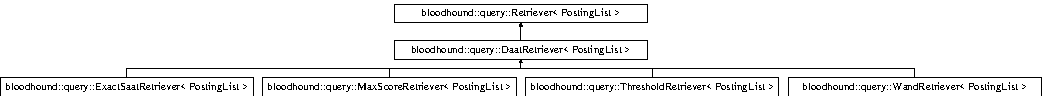
\includegraphics[height=1.296296cm]{classbloodhound_1_1query_1_1DaatRetriever}
\end{center}
\end{figure}
\subsection*{Classes}
\begin{DoxyCompactItemize}
\item 
struct \mbox{\hyperlink{structbloodhound_1_1query_1_1DaatRetriever_1_1IteratorPair}{Iterator\+Pair}}
\begin{DoxyCompactList}\small\item\em Current and end iterators of the same posting list. \end{DoxyCompactList}\end{DoxyCompactItemize}
\subsection*{Public Member Functions}
\begin{DoxyCompactItemize}
\item 
virtual \mbox{\hyperlink{classirk_1_1Heap}{irk\+::\+Heap}}$<$ \mbox{\hyperlink{structbloodhound_1_1Doc}{Doc}}, unsigned int $>$ \mbox{\hyperlink{classbloodhound_1_1query_1_1DaatRetriever_a6c292b0ca9feb30dbdb3a2799a34b3e5}{post\+\_\+lists\+\_\+by\+\_\+doc}} (const std\+::vector$<$ \mbox{\hyperlink{classbloodhound_1_1PostingList}{Posting\+List}} $>$ \&term\+\_\+postings)
\begin{DoxyCompactList}\small\item\em Returns initial min-\/heap of posting lists sorted by their current \mbox{\hyperlink{structbloodhound_1_1Doc}{Doc}}. \end{DoxyCompactList}\item 
virtual std\+::vector$<$ \mbox{\hyperlink{structbloodhound_1_1query_1_1DaatRetriever_1_1IteratorPair}{Iterator\+Pair}} $>$ \mbox{\hyperlink{classbloodhound_1_1query_1_1DaatRetriever_a5b10288f90a4fc4d89f56971bdc48363}{to\+\_\+iterators}} (const std\+::vector$<$ \mbox{\hyperlink{classbloodhound_1_1PostingList}{Posting\+List}} $>$ \&term\+\_\+postings)
\item 
virtual std\+::vector$<$ \mbox{\hyperlink{structbloodhound_1_1query_1_1Result}{Result}} $>$ \mbox{\hyperlink{classbloodhound_1_1query_1_1DaatRetriever_ab80b4867fc263827dc2fdbe0965a2e8c}{retrieve}} (const std\+::vector$<$ \mbox{\hyperlink{classbloodhound_1_1PostingList}{Posting\+List}} $>$ \&term\+\_\+postings, const std\+::vector$<$ \mbox{\hyperlink{structbloodhound_1_1Score}{Score}} $>$ \&term\+\_\+weights, std\+::size\+\_\+t k)
\begin{DoxyCompactList}\small\item\em Retrieves top-\/k results for the given posting lists and term weights. \end{DoxyCompactList}\end{DoxyCompactItemize}


\subsection{Detailed Description}
\subsubsection*{template$<$typename Posting\+List$>$\newline
class bloodhound\+::query\+::\+Daat\+Retriever$<$ Posting\+List $>$}

Document-\/at-\/a-\/time query processor. 

\subsection{Member Function Documentation}
\mbox{\Hypertarget{classbloodhound_1_1query_1_1DaatRetriever_a6c292b0ca9feb30dbdb3a2799a34b3e5}\label{classbloodhound_1_1query_1_1DaatRetriever_a6c292b0ca9feb30dbdb3a2799a34b3e5}} 
\index{bloodhound\+::query\+::\+Daat\+Retriever@{bloodhound\+::query\+::\+Daat\+Retriever}!post\+\_\+lists\+\_\+by\+\_\+doc@{post\+\_\+lists\+\_\+by\+\_\+doc}}
\index{post\+\_\+lists\+\_\+by\+\_\+doc@{post\+\_\+lists\+\_\+by\+\_\+doc}!bloodhound\+::query\+::\+Daat\+Retriever@{bloodhound\+::query\+::\+Daat\+Retriever}}
\subsubsection{\texorpdfstring{post\+\_\+lists\+\_\+by\+\_\+doc()}{post\_lists\_by\_doc()}}
{\footnotesize\ttfamily template$<$typename Posting\+List $>$ \\
virtual \mbox{\hyperlink{classirk_1_1Heap}{irk\+::\+Heap}}$<$\mbox{\hyperlink{structbloodhound_1_1Doc}{Doc}}, unsigned int$>$ \mbox{\hyperlink{classbloodhound_1_1query_1_1DaatRetriever}{bloodhound\+::query\+::\+Daat\+Retriever}}$<$ \mbox{\hyperlink{classbloodhound_1_1PostingList}{Posting\+List}} $>$\+::post\+\_\+lists\+\_\+by\+\_\+doc (\begin{DoxyParamCaption}\item[{const std\+::vector$<$ \mbox{\hyperlink{classbloodhound_1_1PostingList}{Posting\+List}} $>$ \&}]{term\+\_\+postings }\end{DoxyParamCaption})\hspace{0.3cm}{\ttfamily [inline]}, {\ttfamily [virtual]}}



Returns initial min-\/heap of posting lists sorted by their current \mbox{\hyperlink{structbloodhound_1_1Doc}{Doc}}. 

\mbox{\Hypertarget{classbloodhound_1_1query_1_1DaatRetriever_ab80b4867fc263827dc2fdbe0965a2e8c}\label{classbloodhound_1_1query_1_1DaatRetriever_ab80b4867fc263827dc2fdbe0965a2e8c}} 
\index{bloodhound\+::query\+::\+Daat\+Retriever@{bloodhound\+::query\+::\+Daat\+Retriever}!retrieve@{retrieve}}
\index{retrieve@{retrieve}!bloodhound\+::query\+::\+Daat\+Retriever@{bloodhound\+::query\+::\+Daat\+Retriever}}
\subsubsection{\texorpdfstring{retrieve()}{retrieve()}}
{\footnotesize\ttfamily template$<$typename Posting\+List $>$ \\
virtual std\+::vector$<$\mbox{\hyperlink{structbloodhound_1_1query_1_1Result}{Result}}$>$ \mbox{\hyperlink{classbloodhound_1_1query_1_1DaatRetriever}{bloodhound\+::query\+::\+Daat\+Retriever}}$<$ \mbox{\hyperlink{classbloodhound_1_1PostingList}{Posting\+List}} $>$\+::retrieve (\begin{DoxyParamCaption}\item[{const std\+::vector$<$ \mbox{\hyperlink{classbloodhound_1_1PostingList}{Posting\+List}} $>$ \&}]{term\+\_\+postings,  }\item[{const std\+::vector$<$ \mbox{\hyperlink{structbloodhound_1_1Score}{Score}} $>$ \&}]{term\+\_\+weights,  }\item[{std\+::size\+\_\+t}]{k }\end{DoxyParamCaption})\hspace{0.3cm}{\ttfamily [inline]}, {\ttfamily [virtual]}}



Retrieves top-\/k results for the given posting lists and term weights. 



Implements \mbox{\hyperlink{classbloodhound_1_1query_1_1Retriever_ae3c6a4628c5580e620c213b3dcd47c2b}{bloodhound\+::query\+::\+Retriever$<$ Posting\+List $>$}}.



Reimplemented in \mbox{\hyperlink{classbloodhound_1_1query_1_1WandRetriever_a5f3068bc363c16c5b7255a925ea5af8c}{bloodhound\+::query\+::\+Wand\+Retriever$<$ Posting\+List $>$}}, \mbox{\hyperlink{classbloodhound_1_1query_1_1ThresholdRetriever_a06750450e1246e755ebad2d5dac6e8a8}{bloodhound\+::query\+::\+Threshold\+Retriever$<$ Posting\+List $>$}}, and \mbox{\hyperlink{classbloodhound_1_1query_1_1ExactSaatRetriever_aced2763cc2a4c12838fef4a20759049e}{bloodhound\+::query\+::\+Exact\+Saat\+Retriever$<$ Posting\+List $>$}}.

\mbox{\Hypertarget{classbloodhound_1_1query_1_1DaatRetriever_a5b10288f90a4fc4d89f56971bdc48363}\label{classbloodhound_1_1query_1_1DaatRetriever_a5b10288f90a4fc4d89f56971bdc48363}} 
\index{bloodhound\+::query\+::\+Daat\+Retriever@{bloodhound\+::query\+::\+Daat\+Retriever}!to\+\_\+iterators@{to\+\_\+iterators}}
\index{to\+\_\+iterators@{to\+\_\+iterators}!bloodhound\+::query\+::\+Daat\+Retriever@{bloodhound\+::query\+::\+Daat\+Retriever}}
\subsubsection{\texorpdfstring{to\+\_\+iterators()}{to\_iterators()}}
{\footnotesize\ttfamily template$<$typename Posting\+List $>$ \\
virtual std\+::vector$<$\mbox{\hyperlink{structbloodhound_1_1query_1_1DaatRetriever_1_1IteratorPair}{Iterator\+Pair}}$>$ \mbox{\hyperlink{classbloodhound_1_1query_1_1DaatRetriever}{bloodhound\+::query\+::\+Daat\+Retriever}}$<$ \mbox{\hyperlink{classbloodhound_1_1PostingList}{Posting\+List}} $>$\+::to\+\_\+iterators (\begin{DoxyParamCaption}\item[{const std\+::vector$<$ \mbox{\hyperlink{classbloodhound_1_1PostingList}{Posting\+List}} $>$ \&}]{term\+\_\+postings }\end{DoxyParamCaption})\hspace{0.3cm}{\ttfamily [inline]}, {\ttfamily [virtual]}}



The documentation for this class was generated from the following file\+:\begin{DoxyCompactItemize}
\item 
include/\mbox{\hyperlink{retrievers_8hpp}{retrievers.\+hpp}}\end{DoxyCompactItemize}

\hypertarget{structbloodhound_1_1query_1_1debug}{}\section{bloodhound\+:\+:query\+:\+:debug Struct Reference}
\label{structbloodhound_1_1query_1_1debug}\index{bloodhound\+::query\+::debug@{bloodhound\+::query\+::debug}}


{\ttfamily \#include $<$query.\+hpp$>$}

Inheritance diagram for bloodhound\+:\+:query\+:\+:debug\+:\begin{figure}[H]
\begin{center}
\leavevmode
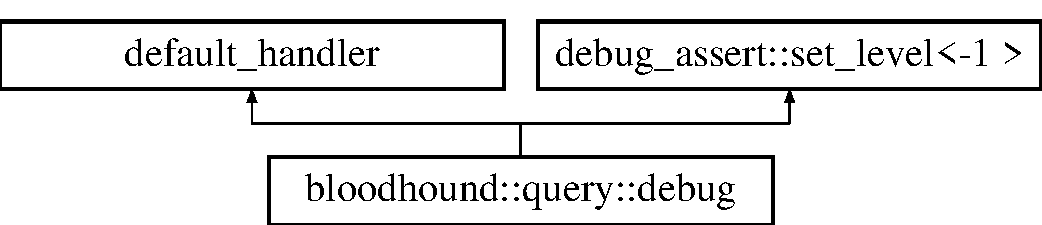
\includegraphics[height=2.000000cm]{structbloodhound_1_1query_1_1debug}
\end{center}
\end{figure}


The documentation for this struct was generated from the following file\+:\begin{DoxyCompactItemize}
\item 
include/\mbox{\hyperlink{query_8hpp}{query.\+hpp}}\end{DoxyCompactItemize}

\hypertarget{structbloodhound_1_1Doc}{}\section{bloodhound\+:\+:Doc Struct Reference}
\label{structbloodhound_1_1Doc}\index{bloodhound\+::\+Doc@{bloodhound\+::\+Doc}}


{\ttfamily \#include $<$index.\+hpp$>$}

Inheritance diagram for bloodhound\+:\+:Doc\+:\begin{figure}[H]
\begin{center}
\leavevmode
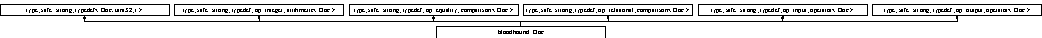
\includegraphics[height=0.514233cm]{structbloodhound_1_1Doc}
\end{center}
\end{figure}
\subsection*{Public Member Functions}
\begin{DoxyCompactItemize}
\item 
\mbox{\hyperlink{structbloodhound_1_1Doc_afb469079253eb5b66e0b613f873ae81d}{operator std\+::size\+\_\+t}} () const
\end{DoxyCompactItemize}


\subsection{Member Function Documentation}
\mbox{\Hypertarget{structbloodhound_1_1Doc_afb469079253eb5b66e0b613f873ae81d}\label{structbloodhound_1_1Doc_afb469079253eb5b66e0b613f873ae81d}} 
\index{bloodhound\+::\+Doc@{bloodhound\+::\+Doc}!operator std\+::size\+\_\+t@{operator std\+::size\+\_\+t}}
\index{operator std\+::size\+\_\+t@{operator std\+::size\+\_\+t}!bloodhound\+::\+Doc@{bloodhound\+::\+Doc}}
\subsubsection{\texorpdfstring{operator std\+::size\+\_\+t()}{operator std::size\_t()}}
{\footnotesize\ttfamily bloodhound\+::\+Doc\+::operator std\+::size\+\_\+t (\begin{DoxyParamCaption}{ }\end{DoxyParamCaption}) const\hspace{0.3cm}{\ttfamily [inline]}}



The documentation for this struct was generated from the following file\+:\begin{DoxyCompactItemize}
\item 
include/\mbox{\hyperlink{index_8hpp}{index.\+hpp}}\end{DoxyCompactItemize}

\hypertarget{structbloodhound_1_1doc__equal__to}{}\section{bloodhound\+:\+:doc\+\_\+equal\+\_\+to$<$ Posting $>$ Struct Template Reference}
\label{structbloodhound_1_1doc__equal__to}\index{bloodhound\+::doc\+\_\+equal\+\_\+to$<$ Posting $>$@{bloodhound\+::doc\+\_\+equal\+\_\+to$<$ Posting $>$}}


{\ttfamily \#include $<$index.\+hpp$>$}

\subsection*{Public Member Functions}
\begin{DoxyCompactItemize}
\item 
bool \mbox{\hyperlink{structbloodhound_1_1doc__equal__to_a5a8e28107bb693527fa4c513b3678b1b}{operator()}} (const \mbox{\hyperlink{structbloodhound_1_1Posting}{Posting}} \&lhs, const \mbox{\hyperlink{structbloodhound_1_1Posting}{Posting}} \&rhs)
\end{DoxyCompactItemize}


\subsection{Member Function Documentation}
\mbox{\Hypertarget{structbloodhound_1_1doc__equal__to_a5a8e28107bb693527fa4c513b3678b1b}\label{structbloodhound_1_1doc__equal__to_a5a8e28107bb693527fa4c513b3678b1b}} 
\index{bloodhound\+::doc\+\_\+equal\+\_\+to@{bloodhound\+::doc\+\_\+equal\+\_\+to}!operator()@{operator()}}
\index{operator()@{operator()}!bloodhound\+::doc\+\_\+equal\+\_\+to@{bloodhound\+::doc\+\_\+equal\+\_\+to}}
\subsubsection{\texorpdfstring{operator()()}{operator()()}}
{\footnotesize\ttfamily template$<$class Posting $>$ \\
bool \mbox{\hyperlink{structbloodhound_1_1doc__equal__to}{bloodhound\+::doc\+\_\+equal\+\_\+to}}$<$ \mbox{\hyperlink{structbloodhound_1_1Posting}{Posting}} $>$\+::operator() (\begin{DoxyParamCaption}\item[{const \mbox{\hyperlink{structbloodhound_1_1Posting}{Posting}} \&}]{lhs,  }\item[{const \mbox{\hyperlink{structbloodhound_1_1Posting}{Posting}} \&}]{rhs }\end{DoxyParamCaption})\hspace{0.3cm}{\ttfamily [inline]}}



The documentation for this struct was generated from the following file\+:\begin{DoxyCompactItemize}
\item 
include/\mbox{\hyperlink{index_8hpp}{index.\+hpp}}\end{DoxyCompactItemize}

\hypertarget{structirkit_1_1UnionRange_1_1docterm}{}\section{irkit\+:\+:Union\+Range$<$ Range $>$\+:\+:docterm Struct Reference}
\label{structirkit_1_1UnionRange_1_1docterm}\index{irkit\+::\+Union\+Range$<$ Range $>$\+::docterm@{irkit\+::\+Union\+Range$<$ Range $>$\+::docterm}}


Pair of document ID and term ID to use in D\+A\+AT term heap.  




{\ttfamily \#include $<$daat.\+hpp$>$}

\subsection*{Public Member Functions}
\begin{DoxyCompactItemize}
\item 
\hyperlink{structirkit_1_1UnionRange_1_1docterm_a5a45bee16d82935e804cf2a0a492a3c5}{docterm} (\hyperlink{classirkit_1_1UnionRange_a387589b1f09868b60485c4ab8c61f97a}{Doc} d, unsigned int t)
\item 
bool \hyperlink{structirkit_1_1UnionRange_1_1docterm_a089cce245934c7558deb5e9405f36e65}{operator==} (const \hyperlink{structirkit_1_1UnionRange_1_1docterm}{docterm} \&rhs) const
\item 
bool \hyperlink{structirkit_1_1UnionRange_1_1docterm_a5f4842c5758933c11d28a00aa5a66262}{operator$<$} (const \hyperlink{structirkit_1_1UnionRange_1_1docterm}{docterm} \&rhs) const
\end{DoxyCompactItemize}
\subsection*{Public Attributes}
\begin{DoxyCompactItemize}
\item 
\hyperlink{classirkit_1_1UnionRange_a387589b1f09868b60485c4ab8c61f97a}{Doc} \hyperlink{structirkit_1_1UnionRange_1_1docterm_a4fe1c3b4721f619f688189d6b5e4afe2}{doc}
\item 
unsigned int \hyperlink{structirkit_1_1UnionRange_1_1docterm_aa8219ac3bc95a63da177aaf0689eaff0}{term}
\end{DoxyCompactItemize}


\subsection{Detailed Description}
\subsubsection*{template$<$class Range$>$\newline
struct irkit\+::\+Union\+Range$<$ Range $>$\+::docterm}

Pair of document ID and term ID to use in D\+A\+AT term heap. 

\subsection{Constructor \& Destructor Documentation}
\mbox{\Hypertarget{structirkit_1_1UnionRange_1_1docterm_a5a45bee16d82935e804cf2a0a492a3c5}\label{structirkit_1_1UnionRange_1_1docterm_a5a45bee16d82935e804cf2a0a492a3c5}} 
\index{irkit\+::\+Union\+Range\+::docterm@{irkit\+::\+Union\+Range\+::docterm}!docterm@{docterm}}
\index{docterm@{docterm}!irkit\+::\+Union\+Range\+::docterm@{irkit\+::\+Union\+Range\+::docterm}}
\subsubsection{\texorpdfstring{docterm()}{docterm()}}
{\footnotesize\ttfamily template$<$class Range $>$ \\
\hyperlink{classirkit_1_1UnionRange}{irkit\+::\+Union\+Range}$<$ Range $>$\+::docterm\+::docterm (\begin{DoxyParamCaption}\item[{\hyperlink{classirkit_1_1UnionRange_a387589b1f09868b60485c4ab8c61f97a}{Doc}}]{d,  }\item[{unsigned int}]{t }\end{DoxyParamCaption})\hspace{0.3cm}{\ttfamily [inline]}}



\subsection{Member Function Documentation}
\mbox{\Hypertarget{structirkit_1_1UnionRange_1_1docterm_a5f4842c5758933c11d28a00aa5a66262}\label{structirkit_1_1UnionRange_1_1docterm_a5f4842c5758933c11d28a00aa5a66262}} 
\index{irkit\+::\+Union\+Range\+::docterm@{irkit\+::\+Union\+Range\+::docterm}!operator$<$@{operator$<$}}
\index{operator$<$@{operator$<$}!irkit\+::\+Union\+Range\+::docterm@{irkit\+::\+Union\+Range\+::docterm}}
\subsubsection{\texorpdfstring{operator$<$()}{operator<()}}
{\footnotesize\ttfamily template$<$class Range $>$ \\
bool \hyperlink{classirkit_1_1UnionRange}{irkit\+::\+Union\+Range}$<$ Range $>$\+::docterm\+::operator$<$ (\begin{DoxyParamCaption}\item[{const \hyperlink{structirkit_1_1UnionRange_1_1docterm}{docterm} \&}]{rhs }\end{DoxyParamCaption}) const\hspace{0.3cm}{\ttfamily [inline]}}

\mbox{\Hypertarget{structirkit_1_1UnionRange_1_1docterm_a089cce245934c7558deb5e9405f36e65}\label{structirkit_1_1UnionRange_1_1docterm_a089cce245934c7558deb5e9405f36e65}} 
\index{irkit\+::\+Union\+Range\+::docterm@{irkit\+::\+Union\+Range\+::docterm}!operator==@{operator==}}
\index{operator==@{operator==}!irkit\+::\+Union\+Range\+::docterm@{irkit\+::\+Union\+Range\+::docterm}}
\subsubsection{\texorpdfstring{operator==()}{operator==()}}
{\footnotesize\ttfamily template$<$class Range $>$ \\
bool \hyperlink{classirkit_1_1UnionRange}{irkit\+::\+Union\+Range}$<$ Range $>$\+::docterm\+::operator== (\begin{DoxyParamCaption}\item[{const \hyperlink{structirkit_1_1UnionRange_1_1docterm}{docterm} \&}]{rhs }\end{DoxyParamCaption}) const\hspace{0.3cm}{\ttfamily [inline]}}



\subsection{Member Data Documentation}
\mbox{\Hypertarget{structirkit_1_1UnionRange_1_1docterm_a4fe1c3b4721f619f688189d6b5e4afe2}\label{structirkit_1_1UnionRange_1_1docterm_a4fe1c3b4721f619f688189d6b5e4afe2}} 
\index{irkit\+::\+Union\+Range\+::docterm@{irkit\+::\+Union\+Range\+::docterm}!doc@{doc}}
\index{doc@{doc}!irkit\+::\+Union\+Range\+::docterm@{irkit\+::\+Union\+Range\+::docterm}}
\subsubsection{\texorpdfstring{doc}{doc}}
{\footnotesize\ttfamily template$<$class Range $>$ \\
\hyperlink{classirkit_1_1UnionRange_a387589b1f09868b60485c4ab8c61f97a}{Doc} \hyperlink{classirkit_1_1UnionRange}{irkit\+::\+Union\+Range}$<$ Range $>$\+::docterm\+::doc}

\mbox{\Hypertarget{structirkit_1_1UnionRange_1_1docterm_aa8219ac3bc95a63da177aaf0689eaff0}\label{structirkit_1_1UnionRange_1_1docterm_aa8219ac3bc95a63da177aaf0689eaff0}} 
\index{irkit\+::\+Union\+Range\+::docterm@{irkit\+::\+Union\+Range\+::docterm}!term@{term}}
\index{term@{term}!irkit\+::\+Union\+Range\+::docterm@{irkit\+::\+Union\+Range\+::docterm}}
\subsubsection{\texorpdfstring{term}{term}}
{\footnotesize\ttfamily template$<$class Range $>$ \\
unsigned int \hyperlink{classirkit_1_1UnionRange}{irkit\+::\+Union\+Range}$<$ Range $>$\+::docterm\+::term}



The documentation for this struct was generated from the following file\+:\begin{DoxyCompactItemize}
\item 
include/irkit/\hyperlink{daat_8hpp}{daat.\+hpp}\end{DoxyCompactItemize}

\hypertarget{classirkit_1_1DynamiclyScoredPostingRange}{}\section{irkit\+:\+:Dynamicly\+Scored\+Posting\+Range$<$ Posting, Freq, Score\+Fn, $>$ Class Template Reference}
\label{classirkit_1_1DynamiclyScoredPostingRange}\index{irkit\+::\+Dynamicly\+Scored\+Posting\+Range$<$ Posting, Freq, Score\+Fn, $>$@{irkit\+::\+Dynamicly\+Scored\+Posting\+Range$<$ Posting, Freq, Score\+Fn, $>$}}


A posting range with scores calculated on the fly.  




{\ttfamily \#include $<$index.\+hpp$>$}

\subsection*{Classes}
\begin{DoxyCompactItemize}
\item 
class \hyperlink{classirkit_1_1DynamiclyScoredPostingRange_1_1iterator}{iterator}
\end{DoxyCompactItemize}
\subsection*{Public Member Functions}
\begin{DoxyCompactItemize}
\item 
\hyperlink{classirkit_1_1DynamiclyScoredPostingRange_a505ae46df58b541505dcc795df5e045d}{Dynamicly\+Scored\+Posting\+Range} (std\+::vector$<$ Doc $>$ \&\&docs, std\+::vector$<$ Freq $>$ \&\&counts, Freq term\+\_\+df, std\+::size\+\_\+t n, Score\+Fn score\+\_\+fn=\hyperlink{structirkit_1_1score_1_1TfIdf}{score\+::\+Tf\+Idf}\{\})
\begin{DoxyCompactList}\small\item\em Constructs a posting range for a term. \end{DoxyCompactList}\item 
\hyperlink{classirkit_1_1DynamiclyScoredPostingRange_1_1iterator}{iterator} \hyperlink{classirkit_1_1DynamiclyScoredPostingRange_a9fe9532cee4feaeefe305e8593f436b6}{cbegin} () const
\item 
\hyperlink{classirkit_1_1DynamiclyScoredPostingRange_1_1iterator}{iterator} \hyperlink{classirkit_1_1DynamiclyScoredPostingRange_a85219c57f0da94d00d1ed1c8f041d976}{cend} () const
\item 
\hyperlink{classirkit_1_1DynamiclyScoredPostingRange_1_1iterator}{iterator} \hyperlink{classirkit_1_1DynamiclyScoredPostingRange_a6a9d369c6e38b5a2b39cbbacb0dc5bed}{begin} () const
\item 
\hyperlink{classirkit_1_1DynamiclyScoredPostingRange_1_1iterator}{iterator} \hyperlink{classirkit_1_1DynamiclyScoredPostingRange_a6d0857abfae0edcf8a2c5d63916dfbb1}{end} () const
\item 
std\+::size\+\_\+t \hyperlink{classirkit_1_1DynamiclyScoredPostingRange_a3a080b946216c0caf02eb9749c8e2e2e}{size} ()
\end{DoxyCompactItemize}


\subsection{Detailed Description}
\subsubsection*{template$<$class Posting, class Freq, class Score\+Fn = score\+::\+Tf\+Idf, C\+O\+N\+C\+E\+P\+T\+\_\+\+R\+E\+Q\+U\+I\+R\+E\+S\+\_\+(ranges\+::\+Integral$<$ Freq $>$())$>$\newline
class irkit\+::\+Dynamicly\+Scored\+Posting\+Range$<$ Posting, Freq, Score\+Fn, $>$}

A posting range with scores calculated on the fly. 


\begin{DoxyTemplParams}{Template Parameters}
{\em Posting} & The posting structure type\+: must have {\ttfamily Posting\+::doc} and {\ttfamily Posting\+::score} members. \\
\hline
{\em Freq} & An integral type of term frequencies. \\
\hline
{\em Score\+Fn} & A scoring function or structure \\
\hline
\end{DoxyTemplParams}


\subsection{Constructor \& Destructor Documentation}
\mbox{\Hypertarget{classirkit_1_1DynamiclyScoredPostingRange_a505ae46df58b541505dcc795df5e045d}\label{classirkit_1_1DynamiclyScoredPostingRange_a505ae46df58b541505dcc795df5e045d}} 
\index{irkit\+::\+Dynamicly\+Scored\+Posting\+Range@{irkit\+::\+Dynamicly\+Scored\+Posting\+Range}!Dynamicly\+Scored\+Posting\+Range@{Dynamicly\+Scored\+Posting\+Range}}
\index{Dynamicly\+Scored\+Posting\+Range@{Dynamicly\+Scored\+Posting\+Range}!irkit\+::\+Dynamicly\+Scored\+Posting\+Range@{irkit\+::\+Dynamicly\+Scored\+Posting\+Range}}
\subsubsection{\texorpdfstring{Dynamicly\+Scored\+Posting\+Range()}{DynamiclyScoredPostingRange()}}
{\footnotesize\ttfamily template$<$class Posting, class Freq, class Score\+Fn = score\+::\+Tf\+Idf, C\+O\+N\+C\+E\+P\+T\+\_\+\+R\+E\+Q\+U\+I\+R\+E\+S\+\_\+(ranges\+::\+Integral$<$ Freq $>$()) $>$ \\
\hyperlink{classirkit_1_1DynamiclyScoredPostingRange}{irkit\+::\+Dynamicly\+Scored\+Posting\+Range}$<$ Posting, Freq, Score\+Fn, $>$\+::\hyperlink{classirkit_1_1DynamiclyScoredPostingRange}{Dynamicly\+Scored\+Posting\+Range} (\begin{DoxyParamCaption}\item[{std\+::vector$<$ Doc $>$ \&\&}]{docs,  }\item[{std\+::vector$<$ Freq $>$ \&\&}]{counts,  }\item[{Freq}]{term\+\_\+df,  }\item[{std\+::size\+\_\+t}]{n,  }\item[{Score\+Fn}]{score\+\_\+fn = {\ttfamily \hyperlink{structirkit_1_1score_1_1TfIdf}{score\+::\+Tf\+Idf}\{\}} }\end{DoxyParamCaption})\hspace{0.3cm}{\ttfamily [inline]}}



Constructs a posting range for a term. 


\begin{DoxyParams}{Parameters}
{\em docs} & Document I\+Ds. \\
\hline
{\em counts} & Occurrences of the term in respective documents. \\
\hline
{\em term\+\_\+df} & The term\textquotesingle{}s document frequency. \\
\hline
{\em n} & The collection size. \\
\hline
{\em score\+\_\+fn} & The scoring function or structure of the structure\+: (Freq tf, Freq df, std\+::size\+\_\+t n) -\/$>$ score\+\_\+t$<$\+Posting$>$ \\
\hline
\end{DoxyParams}


\subsection{Member Function Documentation}
\mbox{\Hypertarget{classirkit_1_1DynamiclyScoredPostingRange_a6a9d369c6e38b5a2b39cbbacb0dc5bed}\label{classirkit_1_1DynamiclyScoredPostingRange_a6a9d369c6e38b5a2b39cbbacb0dc5bed}} 
\index{irkit\+::\+Dynamicly\+Scored\+Posting\+Range@{irkit\+::\+Dynamicly\+Scored\+Posting\+Range}!begin@{begin}}
\index{begin@{begin}!irkit\+::\+Dynamicly\+Scored\+Posting\+Range@{irkit\+::\+Dynamicly\+Scored\+Posting\+Range}}
\subsubsection{\texorpdfstring{begin()}{begin()}}
{\footnotesize\ttfamily template$<$class Posting, class Freq, class Score\+Fn = score\+::\+Tf\+Idf, C\+O\+N\+C\+E\+P\+T\+\_\+\+R\+E\+Q\+U\+I\+R\+E\+S\+\_\+(ranges\+::\+Integral$<$ Freq $>$()) $>$ \\
\hyperlink{classirkit_1_1DynamiclyScoredPostingRange_1_1iterator}{iterator} \hyperlink{classirkit_1_1DynamiclyScoredPostingRange}{irkit\+::\+Dynamicly\+Scored\+Posting\+Range}$<$ Posting, Freq, Score\+Fn, $>$\+::begin (\begin{DoxyParamCaption}{ }\end{DoxyParamCaption}) const\hspace{0.3cm}{\ttfamily [inline]}}

\mbox{\Hypertarget{classirkit_1_1DynamiclyScoredPostingRange_a9fe9532cee4feaeefe305e8593f436b6}\label{classirkit_1_1DynamiclyScoredPostingRange_a9fe9532cee4feaeefe305e8593f436b6}} 
\index{irkit\+::\+Dynamicly\+Scored\+Posting\+Range@{irkit\+::\+Dynamicly\+Scored\+Posting\+Range}!cbegin@{cbegin}}
\index{cbegin@{cbegin}!irkit\+::\+Dynamicly\+Scored\+Posting\+Range@{irkit\+::\+Dynamicly\+Scored\+Posting\+Range}}
\subsubsection{\texorpdfstring{cbegin()}{cbegin()}}
{\footnotesize\ttfamily template$<$class Posting, class Freq, class Score\+Fn = score\+::\+Tf\+Idf, C\+O\+N\+C\+E\+P\+T\+\_\+\+R\+E\+Q\+U\+I\+R\+E\+S\+\_\+(ranges\+::\+Integral$<$ Freq $>$()) $>$ \\
\hyperlink{classirkit_1_1DynamiclyScoredPostingRange_1_1iterator}{iterator} \hyperlink{classirkit_1_1DynamiclyScoredPostingRange}{irkit\+::\+Dynamicly\+Scored\+Posting\+Range}$<$ Posting, Freq, Score\+Fn, $>$\+::cbegin (\begin{DoxyParamCaption}{ }\end{DoxyParamCaption}) const\hspace{0.3cm}{\ttfamily [inline]}}

\mbox{\Hypertarget{classirkit_1_1DynamiclyScoredPostingRange_a85219c57f0da94d00d1ed1c8f041d976}\label{classirkit_1_1DynamiclyScoredPostingRange_a85219c57f0da94d00d1ed1c8f041d976}} 
\index{irkit\+::\+Dynamicly\+Scored\+Posting\+Range@{irkit\+::\+Dynamicly\+Scored\+Posting\+Range}!cend@{cend}}
\index{cend@{cend}!irkit\+::\+Dynamicly\+Scored\+Posting\+Range@{irkit\+::\+Dynamicly\+Scored\+Posting\+Range}}
\subsubsection{\texorpdfstring{cend()}{cend()}}
{\footnotesize\ttfamily template$<$class Posting, class Freq, class Score\+Fn = score\+::\+Tf\+Idf, C\+O\+N\+C\+E\+P\+T\+\_\+\+R\+E\+Q\+U\+I\+R\+E\+S\+\_\+(ranges\+::\+Integral$<$ Freq $>$()) $>$ \\
\hyperlink{classirkit_1_1DynamiclyScoredPostingRange_1_1iterator}{iterator} \hyperlink{classirkit_1_1DynamiclyScoredPostingRange}{irkit\+::\+Dynamicly\+Scored\+Posting\+Range}$<$ Posting, Freq, Score\+Fn, $>$\+::cend (\begin{DoxyParamCaption}{ }\end{DoxyParamCaption}) const\hspace{0.3cm}{\ttfamily [inline]}}

\mbox{\Hypertarget{classirkit_1_1DynamiclyScoredPostingRange_a6d0857abfae0edcf8a2c5d63916dfbb1}\label{classirkit_1_1DynamiclyScoredPostingRange_a6d0857abfae0edcf8a2c5d63916dfbb1}} 
\index{irkit\+::\+Dynamicly\+Scored\+Posting\+Range@{irkit\+::\+Dynamicly\+Scored\+Posting\+Range}!end@{end}}
\index{end@{end}!irkit\+::\+Dynamicly\+Scored\+Posting\+Range@{irkit\+::\+Dynamicly\+Scored\+Posting\+Range}}
\subsubsection{\texorpdfstring{end()}{end()}}
{\footnotesize\ttfamily template$<$class Posting, class Freq, class Score\+Fn = score\+::\+Tf\+Idf, C\+O\+N\+C\+E\+P\+T\+\_\+\+R\+E\+Q\+U\+I\+R\+E\+S\+\_\+(ranges\+::\+Integral$<$ Freq $>$()) $>$ \\
\hyperlink{classirkit_1_1DynamiclyScoredPostingRange_1_1iterator}{iterator} \hyperlink{classirkit_1_1DynamiclyScoredPostingRange}{irkit\+::\+Dynamicly\+Scored\+Posting\+Range}$<$ Posting, Freq, Score\+Fn, $>$\+::end (\begin{DoxyParamCaption}{ }\end{DoxyParamCaption}) const\hspace{0.3cm}{\ttfamily [inline]}}

\mbox{\Hypertarget{classirkit_1_1DynamiclyScoredPostingRange_a3a080b946216c0caf02eb9749c8e2e2e}\label{classirkit_1_1DynamiclyScoredPostingRange_a3a080b946216c0caf02eb9749c8e2e2e}} 
\index{irkit\+::\+Dynamicly\+Scored\+Posting\+Range@{irkit\+::\+Dynamicly\+Scored\+Posting\+Range}!size@{size}}
\index{size@{size}!irkit\+::\+Dynamicly\+Scored\+Posting\+Range@{irkit\+::\+Dynamicly\+Scored\+Posting\+Range}}
\subsubsection{\texorpdfstring{size()}{size()}}
{\footnotesize\ttfamily template$<$class Posting, class Freq, class Score\+Fn = score\+::\+Tf\+Idf, C\+O\+N\+C\+E\+P\+T\+\_\+\+R\+E\+Q\+U\+I\+R\+E\+S\+\_\+(ranges\+::\+Integral$<$ Freq $>$()) $>$ \\
std\+::size\+\_\+t \hyperlink{classirkit_1_1DynamiclyScoredPostingRange}{irkit\+::\+Dynamicly\+Scored\+Posting\+Range}$<$ Posting, Freq, Score\+Fn, $>$\+::size (\begin{DoxyParamCaption}{ }\end{DoxyParamCaption})\hspace{0.3cm}{\ttfamily [inline]}}



The documentation for this class was generated from the following file\+:\begin{DoxyCompactItemize}
\item 
include/irkit/\hyperlink{irkit_2index_8hpp}{index.\+hpp}\end{DoxyCompactItemize}

\hypertarget{classirkit_1_1EmptyMapping}{}\section{irkit\+:\+:Empty\+Mapping Class Reference}
\label{classirkit_1_1EmptyMapping}\index{irkit\+::\+Empty\+Mapping@{irkit\+::\+Empty\+Mapping}}


{\ttfamily \#include $<$heap.\+hpp$>$}



The documentation for this class was generated from the following file\+:\begin{DoxyCompactItemize}
\item 
include/irkit/\hyperlink{heap_8hpp}{heap.\+hpp}\end{DoxyCompactItemize}

\hypertarget{structirkit_1_1Entry}{}\section{irkit\+:\+:Entry$<$ Key, Value $>$ Struct Template Reference}
\label{structirkit_1_1Entry}\index{irkit\+::\+Entry$<$ Key, Value $>$@{irkit\+::\+Entry$<$ Key, Value $>$}}


The type of objects stored internally in the heap.  




{\ttfamily \#include $<$heap.\+hpp$>$}

\subsection*{Public Member Functions}
\begin{DoxyCompactItemize}
\item 
\mbox{\hyperlink{structirkit_1_1Entry_ab8d6ae4f3f3ff0c1934543f2eca895ea}{Entry}} ()=default
\item 
\mbox{\hyperlink{structirkit_1_1Entry_afe9a7f9975902c4622115176169bc80a}{Entry}} (Key \mbox{\hyperlink{structirkit_1_1Entry_aeae4387483b4905afd7dfd71df9104fc}{key}}, Value \mbox{\hyperlink{structirkit_1_1Entry_a72e5dd8efe13d360f7b97c37d05b99b8}{value}})
\item 
bool \mbox{\hyperlink{structirkit_1_1Entry_aaa12df0ae7e66638a6f0e5ddb552167b}{operator==}} (const \mbox{\hyperlink{structirkit_1_1Entry}{Entry}} \&rhs) const
\item 
bool \mbox{\hyperlink{structirkit_1_1Entry_a4112e1db14a84edfe80b4e75ed8a328c}{operator$<$}} (const \mbox{\hyperlink{structirkit_1_1Entry}{Entry}} \&rhs) const
\item 
bool \mbox{\hyperlink{structirkit_1_1Entry_a0c421723ffe0eb3c56d1efc16f5f2fe5}{operator$>$}} (const \mbox{\hyperlink{structirkit_1_1Entry}{Entry}} \&rhs) const
\item 
bool \mbox{\hyperlink{structirkit_1_1Entry_aa84e1aed3325a2c1bfef85b71a20ed74}{operator$<$=}} (const \mbox{\hyperlink{structirkit_1_1Entry}{Entry}} \&rhs) const
\item 
bool \mbox{\hyperlink{structirkit_1_1Entry_a672de7d54aa88d29475e8664422a8e4f}{operator$>$=}} (const \mbox{\hyperlink{structirkit_1_1Entry}{Entry}} \&rhs) const
\end{DoxyCompactItemize}
\subsection*{Public Attributes}
\begin{DoxyCompactItemize}
\item 
Key \mbox{\hyperlink{structirkit_1_1Entry_aeae4387483b4905afd7dfd71df9104fc}{key}}
\item 
Value \mbox{\hyperlink{structirkit_1_1Entry_a72e5dd8efe13d360f7b97c37d05b99b8}{value}}
\end{DoxyCompactItemize}
\subsection*{Friends}
\begin{DoxyCompactItemize}
\item 
std\+::ostream \& \mbox{\hyperlink{structirkit_1_1Entry_a885f1645de32df3dbfbf9f2f47f7ea1f}{operator$<$$<$}} (std\+::ostream \&os, \mbox{\hyperlink{structirkit_1_1Entry}{Entry}} \&he)
\end{DoxyCompactItemize}


\subsection{Detailed Description}
\subsubsection*{template$<$class Key, class Value$>$\newline
struct irkit\+::\+Entry$<$ Key, Value $>$}

The type of objects stored internally in the heap. 

\subsection{Constructor \& Destructor Documentation}
\mbox{\Hypertarget{structirkit_1_1Entry_ab8d6ae4f3f3ff0c1934543f2eca895ea}\label{structirkit_1_1Entry_ab8d6ae4f3f3ff0c1934543f2eca895ea}} 
\index{irkit\+::\+Entry@{irkit\+::\+Entry}!Entry@{Entry}}
\index{Entry@{Entry}!irkit\+::\+Entry@{irkit\+::\+Entry}}
\subsubsection{\texorpdfstring{Entry()}{Entry()}\hspace{0.1cm}{\footnotesize\ttfamily [1/2]}}
{\footnotesize\ttfamily template$<$class Key, class Value$>$ \\
\mbox{\hyperlink{structirkit_1_1Entry}{irkit\+::\+Entry}}$<$ Key, Value $>$\+::\mbox{\hyperlink{structirkit_1_1Entry}{Entry}} (\begin{DoxyParamCaption}{ }\end{DoxyParamCaption})\hspace{0.3cm}{\ttfamily [default]}}

\mbox{\Hypertarget{structirkit_1_1Entry_afe9a7f9975902c4622115176169bc80a}\label{structirkit_1_1Entry_afe9a7f9975902c4622115176169bc80a}} 
\index{irkit\+::\+Entry@{irkit\+::\+Entry}!Entry@{Entry}}
\index{Entry@{Entry}!irkit\+::\+Entry@{irkit\+::\+Entry}}
\subsubsection{\texorpdfstring{Entry()}{Entry()}\hspace{0.1cm}{\footnotesize\ttfamily [2/2]}}
{\footnotesize\ttfamily template$<$class Key, class Value$>$ \\
\mbox{\hyperlink{structirkit_1_1Entry}{irkit\+::\+Entry}}$<$ Key, Value $>$\+::\mbox{\hyperlink{structirkit_1_1Entry}{Entry}} (\begin{DoxyParamCaption}\item[{Key}]{key,  }\item[{Value}]{value }\end{DoxyParamCaption})\hspace{0.3cm}{\ttfamily [inline]}}



\subsection{Member Function Documentation}
\mbox{\Hypertarget{structirkit_1_1Entry_a4112e1db14a84edfe80b4e75ed8a328c}\label{structirkit_1_1Entry_a4112e1db14a84edfe80b4e75ed8a328c}} 
\index{irkit\+::\+Entry@{irkit\+::\+Entry}!operator$<$@{operator$<$}}
\index{operator$<$@{operator$<$}!irkit\+::\+Entry@{irkit\+::\+Entry}}
\subsubsection{\texorpdfstring{operator$<$()}{operator<()}}
{\footnotesize\ttfamily template$<$class Key, class Value$>$ \\
bool \mbox{\hyperlink{structirkit_1_1Entry}{irkit\+::\+Entry}}$<$ Key, Value $>$\+::operator$<$ (\begin{DoxyParamCaption}\item[{const \mbox{\hyperlink{structirkit_1_1Entry}{Entry}}$<$ Key, Value $>$ \&}]{rhs }\end{DoxyParamCaption}) const\hspace{0.3cm}{\ttfamily [inline]}}

\mbox{\Hypertarget{structirkit_1_1Entry_aa84e1aed3325a2c1bfef85b71a20ed74}\label{structirkit_1_1Entry_aa84e1aed3325a2c1bfef85b71a20ed74}} 
\index{irkit\+::\+Entry@{irkit\+::\+Entry}!operator$<$=@{operator$<$=}}
\index{operator$<$=@{operator$<$=}!irkit\+::\+Entry@{irkit\+::\+Entry}}
\subsubsection{\texorpdfstring{operator$<$=()}{operator<=()}}
{\footnotesize\ttfamily template$<$class Key, class Value$>$ \\
bool \mbox{\hyperlink{structirkit_1_1Entry}{irkit\+::\+Entry}}$<$ Key, Value $>$\+::operator$<$= (\begin{DoxyParamCaption}\item[{const \mbox{\hyperlink{structirkit_1_1Entry}{Entry}}$<$ Key, Value $>$ \&}]{rhs }\end{DoxyParamCaption}) const\hspace{0.3cm}{\ttfamily [inline]}}

\mbox{\Hypertarget{structirkit_1_1Entry_aaa12df0ae7e66638a6f0e5ddb552167b}\label{structirkit_1_1Entry_aaa12df0ae7e66638a6f0e5ddb552167b}} 
\index{irkit\+::\+Entry@{irkit\+::\+Entry}!operator==@{operator==}}
\index{operator==@{operator==}!irkit\+::\+Entry@{irkit\+::\+Entry}}
\subsubsection{\texorpdfstring{operator==()}{operator==()}}
{\footnotesize\ttfamily template$<$class Key, class Value$>$ \\
bool \mbox{\hyperlink{structirkit_1_1Entry}{irkit\+::\+Entry}}$<$ Key, Value $>$\+::operator== (\begin{DoxyParamCaption}\item[{const \mbox{\hyperlink{structirkit_1_1Entry}{Entry}}$<$ Key, Value $>$ \&}]{rhs }\end{DoxyParamCaption}) const\hspace{0.3cm}{\ttfamily [inline]}}

\mbox{\Hypertarget{structirkit_1_1Entry_a0c421723ffe0eb3c56d1efc16f5f2fe5}\label{structirkit_1_1Entry_a0c421723ffe0eb3c56d1efc16f5f2fe5}} 
\index{irkit\+::\+Entry@{irkit\+::\+Entry}!operator$>$@{operator$>$}}
\index{operator$>$@{operator$>$}!irkit\+::\+Entry@{irkit\+::\+Entry}}
\subsubsection{\texorpdfstring{operator$>$()}{operator>()}}
{\footnotesize\ttfamily template$<$class Key, class Value$>$ \\
bool \mbox{\hyperlink{structirkit_1_1Entry}{irkit\+::\+Entry}}$<$ Key, Value $>$\+::operator$>$ (\begin{DoxyParamCaption}\item[{const \mbox{\hyperlink{structirkit_1_1Entry}{Entry}}$<$ Key, Value $>$ \&}]{rhs }\end{DoxyParamCaption}) const\hspace{0.3cm}{\ttfamily [inline]}}

\mbox{\Hypertarget{structirkit_1_1Entry_a672de7d54aa88d29475e8664422a8e4f}\label{structirkit_1_1Entry_a672de7d54aa88d29475e8664422a8e4f}} 
\index{irkit\+::\+Entry@{irkit\+::\+Entry}!operator$>$=@{operator$>$=}}
\index{operator$>$=@{operator$>$=}!irkit\+::\+Entry@{irkit\+::\+Entry}}
\subsubsection{\texorpdfstring{operator$>$=()}{operator>=()}}
{\footnotesize\ttfamily template$<$class Key, class Value$>$ \\
bool \mbox{\hyperlink{structirkit_1_1Entry}{irkit\+::\+Entry}}$<$ Key, Value $>$\+::operator$>$= (\begin{DoxyParamCaption}\item[{const \mbox{\hyperlink{structirkit_1_1Entry}{Entry}}$<$ Key, Value $>$ \&}]{rhs }\end{DoxyParamCaption}) const\hspace{0.3cm}{\ttfamily [inline]}}



\subsection{Friends And Related Function Documentation}
\mbox{\Hypertarget{structirkit_1_1Entry_a885f1645de32df3dbfbf9f2f47f7ea1f}\label{structirkit_1_1Entry_a885f1645de32df3dbfbf9f2f47f7ea1f}} 
\index{irkit\+::\+Entry@{irkit\+::\+Entry}!operator$<$$<$@{operator$<$$<$}}
\index{operator$<$$<$@{operator$<$$<$}!irkit\+::\+Entry@{irkit\+::\+Entry}}
\subsubsection{\texorpdfstring{operator$<$$<$}{operator<<}}
{\footnotesize\ttfamily template$<$class Key, class Value$>$ \\
std\+::ostream\& operator$<$$<$ (\begin{DoxyParamCaption}\item[{std\+::ostream \&}]{os,  }\item[{\mbox{\hyperlink{structirkit_1_1Entry}{Entry}}$<$ Key, Value $>$ \&}]{he }\end{DoxyParamCaption})\hspace{0.3cm}{\ttfamily [friend]}}



\subsection{Member Data Documentation}
\mbox{\Hypertarget{structirkit_1_1Entry_aeae4387483b4905afd7dfd71df9104fc}\label{structirkit_1_1Entry_aeae4387483b4905afd7dfd71df9104fc}} 
\index{irkit\+::\+Entry@{irkit\+::\+Entry}!key@{key}}
\index{key@{key}!irkit\+::\+Entry@{irkit\+::\+Entry}}
\subsubsection{\texorpdfstring{key}{key}}
{\footnotesize\ttfamily template$<$class Key, class Value$>$ \\
Key \mbox{\hyperlink{structirkit_1_1Entry}{irkit\+::\+Entry}}$<$ Key, Value $>$\+::key}

\mbox{\Hypertarget{structirkit_1_1Entry_a72e5dd8efe13d360f7b97c37d05b99b8}\label{structirkit_1_1Entry_a72e5dd8efe13d360f7b97c37d05b99b8}} 
\index{irkit\+::\+Entry@{irkit\+::\+Entry}!value@{value}}
\index{value@{value}!irkit\+::\+Entry@{irkit\+::\+Entry}}
\subsubsection{\texorpdfstring{value}{value}}
{\footnotesize\ttfamily template$<$class Key, class Value$>$ \\
Value \mbox{\hyperlink{structirkit_1_1Entry}{irkit\+::\+Entry}}$<$ Key, Value $>$\+::value}



The documentation for this struct was generated from the following file\+:\begin{DoxyCompactItemize}
\item 
include/irkit/\mbox{\hyperlink{heap_8hpp}{heap.\+hpp}}\end{DoxyCompactItemize}

\hypertarget{classbloodhound_1_1query_1_1ExactSaatRetriever}{}\section{bloodhound\+:\+:query\+:\+:Exact\+Saat\+Retriever$<$ Posting\+List $>$ Class Template Reference}
\label{classbloodhound_1_1query_1_1ExactSaatRetriever}\index{bloodhound\+::query\+::\+Exact\+Saat\+Retriever$<$ Posting\+List $>$@{bloodhound\+::query\+::\+Exact\+Saat\+Retriever$<$ Posting\+List $>$}}


{\ttfamily \#include $<$saat.\+hpp$>$}

Inheritance diagram for bloodhound\+:\+:query\+:\+:Exact\+Saat\+Retriever$<$ Posting\+List $>$\+:\begin{figure}[H]
\begin{center}
\leavevmode
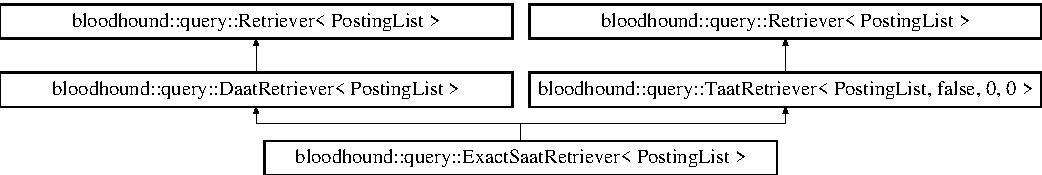
\includegraphics[height=2.346369cm]{classbloodhound_1_1query_1_1ExactSaatRetriever}
\end{center}
\end{figure}
\subsection*{Public Member Functions}
\begin{DoxyCompactItemize}
\item 
\hyperlink{classbloodhound_1_1query_1_1ExactSaatRetriever_a50c5c53b4b7aff76e4eabf040219be52}{Exact\+Saat\+Retriever} (std\+::size\+\_\+t collection\+\_\+size, double et\+\_\+threshold=1.\+0)
\item 
std\+::size\+\_\+t \hyperlink{classbloodhound_1_1query_1_1ExactSaatRetriever_a21f4192190392fee8d8b12b99c6bbe0e}{count\+\_\+postings} (const std\+::vector$<$ \hyperlink{classbloodhound_1_1PostingList}{Posting\+List} $>$ \&term\+\_\+postings)
\item 
virtual irkit\+::\+Heap$<$ \hyperlink{structbloodhound_1_1Score}{Score}, unsigned int $>$ \hyperlink{classbloodhound_1_1query_1_1ExactSaatRetriever_a180277ad96862e92c102066586edc74f}{post\+\_\+lists\+\_\+by\+\_\+score} (const std\+::vector$<$ \hyperlink{classbloodhound_1_1PostingList}{Posting\+List} $>$ \&term\+\_\+postings, const std\+::vector$<$ \hyperlink{structbloodhound_1_1Score}{Score} $>$ \&term\+\_\+weights)
\item 
virtual std\+::vector$<$ \hyperlink{structbloodhound_1_1query_1_1Result}{Result} $>$ \hyperlink{classbloodhound_1_1query_1_1ExactSaatRetriever_aced2763cc2a4c12838fef4a20759049e}{retrieve} (const std\+::vector$<$ \hyperlink{classbloodhound_1_1PostingList}{Posting\+List} $>$ \&term\+\_\+postings, const std\+::vector$<$ \hyperlink{structbloodhound_1_1Score}{Score} $>$ \&term\+\_\+weights, std\+::size\+\_\+t k)
\begin{DoxyCompactList}\small\item\em Retrieves top-\/k results for the given posting lists and term weights. \end{DoxyCompactList}\item 
std\+::size\+\_\+t \hyperlink{classbloodhound_1_1query_1_1ExactSaatRetriever_a1cf3c5e50a72880e1eb8d995ff22b20a}{get\+\_\+processed\+\_\+postings} ()
\item 
std\+::size\+\_\+t \hyperlink{classbloodhound_1_1query_1_1ExactSaatRetriever_a5d3a882f8f117130a4be46e711397e3c}{get\+\_\+posting\+\_\+threshold} ()
\item 
std\+::size\+\_\+t \hyperlink{classbloodhound_1_1query_1_1ExactSaatRetriever_a43b6bd8cdc3a64c5eabf778230c53419}{get\+\_\+posting\+\_\+count} ()
\item 
void \hyperlink{classbloodhound_1_1query_1_1ExactSaatRetriever_a78016cfffe921ed440dec62c6f82f4cc}{set\+\_\+et\+\_\+threshold} (double et)
\item 
virtual nlohmann\+::json \hyperlink{classbloodhound_1_1query_1_1ExactSaatRetriever_a716838f463f124964e76f48bc37d32cc}{stats} ()
\end{DoxyCompactItemize}
\subsection*{Additional Inherited Members}


\subsection{Constructor \& Destructor Documentation}
\mbox{\Hypertarget{classbloodhound_1_1query_1_1ExactSaatRetriever_a50c5c53b4b7aff76e4eabf040219be52}\label{classbloodhound_1_1query_1_1ExactSaatRetriever_a50c5c53b4b7aff76e4eabf040219be52}} 
\index{bloodhound\+::query\+::\+Exact\+Saat\+Retriever@{bloodhound\+::query\+::\+Exact\+Saat\+Retriever}!Exact\+Saat\+Retriever@{Exact\+Saat\+Retriever}}
\index{Exact\+Saat\+Retriever@{Exact\+Saat\+Retriever}!bloodhound\+::query\+::\+Exact\+Saat\+Retriever@{bloodhound\+::query\+::\+Exact\+Saat\+Retriever}}
\subsubsection{\texorpdfstring{Exact\+Saat\+Retriever()}{ExactSaatRetriever()}}
{\footnotesize\ttfamily template$<$typename Posting\+List $>$ \\
\hyperlink{classbloodhound_1_1query_1_1ExactSaatRetriever}{bloodhound\+::query\+::\+Exact\+Saat\+Retriever}$<$ \hyperlink{classbloodhound_1_1PostingList}{Posting\+List} $>$\+::\hyperlink{classbloodhound_1_1query_1_1ExactSaatRetriever}{Exact\+Saat\+Retriever} (\begin{DoxyParamCaption}\item[{std\+::size\+\_\+t}]{collection\+\_\+size,  }\item[{double}]{et\+\_\+threshold = {\ttfamily 1.0} }\end{DoxyParamCaption})\hspace{0.3cm}{\ttfamily [inline]}}



\subsection{Member Function Documentation}
\mbox{\Hypertarget{classbloodhound_1_1query_1_1ExactSaatRetriever_a21f4192190392fee8d8b12b99c6bbe0e}\label{classbloodhound_1_1query_1_1ExactSaatRetriever_a21f4192190392fee8d8b12b99c6bbe0e}} 
\index{bloodhound\+::query\+::\+Exact\+Saat\+Retriever@{bloodhound\+::query\+::\+Exact\+Saat\+Retriever}!count\+\_\+postings@{count\+\_\+postings}}
\index{count\+\_\+postings@{count\+\_\+postings}!bloodhound\+::query\+::\+Exact\+Saat\+Retriever@{bloodhound\+::query\+::\+Exact\+Saat\+Retriever}}
\subsubsection{\texorpdfstring{count\+\_\+postings()}{count\_postings()}}
{\footnotesize\ttfamily template$<$typename Posting\+List $>$ \\
std\+::size\+\_\+t \hyperlink{classbloodhound_1_1query_1_1ExactSaatRetriever}{bloodhound\+::query\+::\+Exact\+Saat\+Retriever}$<$ \hyperlink{classbloodhound_1_1PostingList}{Posting\+List} $>$\+::count\+\_\+postings (\begin{DoxyParamCaption}\item[{const std\+::vector$<$ \hyperlink{classbloodhound_1_1PostingList}{Posting\+List} $>$ \&}]{term\+\_\+postings }\end{DoxyParamCaption})\hspace{0.3cm}{\ttfamily [inline]}}

\mbox{\Hypertarget{classbloodhound_1_1query_1_1ExactSaatRetriever_a43b6bd8cdc3a64c5eabf778230c53419}\label{classbloodhound_1_1query_1_1ExactSaatRetriever_a43b6bd8cdc3a64c5eabf778230c53419}} 
\index{bloodhound\+::query\+::\+Exact\+Saat\+Retriever@{bloodhound\+::query\+::\+Exact\+Saat\+Retriever}!get\+\_\+posting\+\_\+count@{get\+\_\+posting\+\_\+count}}
\index{get\+\_\+posting\+\_\+count@{get\+\_\+posting\+\_\+count}!bloodhound\+::query\+::\+Exact\+Saat\+Retriever@{bloodhound\+::query\+::\+Exact\+Saat\+Retriever}}
\subsubsection{\texorpdfstring{get\+\_\+posting\+\_\+count()}{get\_posting\_count()}}
{\footnotesize\ttfamily template$<$typename Posting\+List $>$ \\
std\+::size\+\_\+t \hyperlink{classbloodhound_1_1query_1_1ExactSaatRetriever}{bloodhound\+::query\+::\+Exact\+Saat\+Retriever}$<$ \hyperlink{classbloodhound_1_1PostingList}{Posting\+List} $>$\+::get\+\_\+posting\+\_\+count (\begin{DoxyParamCaption}{ }\end{DoxyParamCaption})\hspace{0.3cm}{\ttfamily [inline]}}

\mbox{\Hypertarget{classbloodhound_1_1query_1_1ExactSaatRetriever_a5d3a882f8f117130a4be46e711397e3c}\label{classbloodhound_1_1query_1_1ExactSaatRetriever_a5d3a882f8f117130a4be46e711397e3c}} 
\index{bloodhound\+::query\+::\+Exact\+Saat\+Retriever@{bloodhound\+::query\+::\+Exact\+Saat\+Retriever}!get\+\_\+posting\+\_\+threshold@{get\+\_\+posting\+\_\+threshold}}
\index{get\+\_\+posting\+\_\+threshold@{get\+\_\+posting\+\_\+threshold}!bloodhound\+::query\+::\+Exact\+Saat\+Retriever@{bloodhound\+::query\+::\+Exact\+Saat\+Retriever}}
\subsubsection{\texorpdfstring{get\+\_\+posting\+\_\+threshold()}{get\_posting\_threshold()}}
{\footnotesize\ttfamily template$<$typename Posting\+List $>$ \\
std\+::size\+\_\+t \hyperlink{classbloodhound_1_1query_1_1ExactSaatRetriever}{bloodhound\+::query\+::\+Exact\+Saat\+Retriever}$<$ \hyperlink{classbloodhound_1_1PostingList}{Posting\+List} $>$\+::get\+\_\+posting\+\_\+threshold (\begin{DoxyParamCaption}{ }\end{DoxyParamCaption})\hspace{0.3cm}{\ttfamily [inline]}}

\mbox{\Hypertarget{classbloodhound_1_1query_1_1ExactSaatRetriever_a1cf3c5e50a72880e1eb8d995ff22b20a}\label{classbloodhound_1_1query_1_1ExactSaatRetriever_a1cf3c5e50a72880e1eb8d995ff22b20a}} 
\index{bloodhound\+::query\+::\+Exact\+Saat\+Retriever@{bloodhound\+::query\+::\+Exact\+Saat\+Retriever}!get\+\_\+processed\+\_\+postings@{get\+\_\+processed\+\_\+postings}}
\index{get\+\_\+processed\+\_\+postings@{get\+\_\+processed\+\_\+postings}!bloodhound\+::query\+::\+Exact\+Saat\+Retriever@{bloodhound\+::query\+::\+Exact\+Saat\+Retriever}}
\subsubsection{\texorpdfstring{get\+\_\+processed\+\_\+postings()}{get\_processed\_postings()}}
{\footnotesize\ttfamily template$<$typename Posting\+List $>$ \\
std\+::size\+\_\+t \hyperlink{classbloodhound_1_1query_1_1ExactSaatRetriever}{bloodhound\+::query\+::\+Exact\+Saat\+Retriever}$<$ \hyperlink{classbloodhound_1_1PostingList}{Posting\+List} $>$\+::get\+\_\+processed\+\_\+postings (\begin{DoxyParamCaption}{ }\end{DoxyParamCaption})\hspace{0.3cm}{\ttfamily [inline]}}

\mbox{\Hypertarget{classbloodhound_1_1query_1_1ExactSaatRetriever_a180277ad96862e92c102066586edc74f}\label{classbloodhound_1_1query_1_1ExactSaatRetriever_a180277ad96862e92c102066586edc74f}} 
\index{bloodhound\+::query\+::\+Exact\+Saat\+Retriever@{bloodhound\+::query\+::\+Exact\+Saat\+Retriever}!post\+\_\+lists\+\_\+by\+\_\+score@{post\+\_\+lists\+\_\+by\+\_\+score}}
\index{post\+\_\+lists\+\_\+by\+\_\+score@{post\+\_\+lists\+\_\+by\+\_\+score}!bloodhound\+::query\+::\+Exact\+Saat\+Retriever@{bloodhound\+::query\+::\+Exact\+Saat\+Retriever}}
\subsubsection{\texorpdfstring{post\+\_\+lists\+\_\+by\+\_\+score()}{post\_lists\_by\_score()}}
{\footnotesize\ttfamily template$<$typename Posting\+List $>$ \\
virtual irkit\+::\+Heap$<$\hyperlink{structbloodhound_1_1Score}{Score}, unsigned int$>$ \hyperlink{classbloodhound_1_1query_1_1ExactSaatRetriever}{bloodhound\+::query\+::\+Exact\+Saat\+Retriever}$<$ \hyperlink{classbloodhound_1_1PostingList}{Posting\+List} $>$\+::post\+\_\+lists\+\_\+by\+\_\+score (\begin{DoxyParamCaption}\item[{const std\+::vector$<$ \hyperlink{classbloodhound_1_1PostingList}{Posting\+List} $>$ \&}]{term\+\_\+postings,  }\item[{const std\+::vector$<$ \hyperlink{structbloodhound_1_1Score}{Score} $>$ \&}]{term\+\_\+weights }\end{DoxyParamCaption})\hspace{0.3cm}{\ttfamily [inline]}, {\ttfamily [virtual]}}

\mbox{\Hypertarget{classbloodhound_1_1query_1_1ExactSaatRetriever_aced2763cc2a4c12838fef4a20759049e}\label{classbloodhound_1_1query_1_1ExactSaatRetriever_aced2763cc2a4c12838fef4a20759049e}} 
\index{bloodhound\+::query\+::\+Exact\+Saat\+Retriever@{bloodhound\+::query\+::\+Exact\+Saat\+Retriever}!retrieve@{retrieve}}
\index{retrieve@{retrieve}!bloodhound\+::query\+::\+Exact\+Saat\+Retriever@{bloodhound\+::query\+::\+Exact\+Saat\+Retriever}}
\subsubsection{\texorpdfstring{retrieve()}{retrieve()}}
{\footnotesize\ttfamily template$<$typename Posting\+List $>$ \\
virtual std\+::vector$<$\hyperlink{structbloodhound_1_1query_1_1Result}{Result}$>$ \hyperlink{classbloodhound_1_1query_1_1ExactSaatRetriever}{bloodhound\+::query\+::\+Exact\+Saat\+Retriever}$<$ \hyperlink{classbloodhound_1_1PostingList}{Posting\+List} $>$\+::retrieve (\begin{DoxyParamCaption}\item[{const std\+::vector$<$ \hyperlink{classbloodhound_1_1PostingList}{Posting\+List} $>$ \&}]{term\+\_\+postings,  }\item[{const std\+::vector$<$ \hyperlink{structbloodhound_1_1Score}{Score} $>$ \&}]{term\+\_\+weights,  }\item[{std\+::size\+\_\+t}]{k }\end{DoxyParamCaption})\hspace{0.3cm}{\ttfamily [inline]}, {\ttfamily [virtual]}}



Retrieves top-\/k results for the given posting lists and term weights. 



Reimplemented from \hyperlink{classbloodhound_1_1query_1_1DaatRetriever_ab80b4867fc263827dc2fdbe0965a2e8c}{bloodhound\+::query\+::\+Daat\+Retriever$<$ Posting\+List $>$}.

\mbox{\Hypertarget{classbloodhound_1_1query_1_1ExactSaatRetriever_a78016cfffe921ed440dec62c6f82f4cc}\label{classbloodhound_1_1query_1_1ExactSaatRetriever_a78016cfffe921ed440dec62c6f82f4cc}} 
\index{bloodhound\+::query\+::\+Exact\+Saat\+Retriever@{bloodhound\+::query\+::\+Exact\+Saat\+Retriever}!set\+\_\+et\+\_\+threshold@{set\+\_\+et\+\_\+threshold}}
\index{set\+\_\+et\+\_\+threshold@{set\+\_\+et\+\_\+threshold}!bloodhound\+::query\+::\+Exact\+Saat\+Retriever@{bloodhound\+::query\+::\+Exact\+Saat\+Retriever}}
\subsubsection{\texorpdfstring{set\+\_\+et\+\_\+threshold()}{set\_et\_threshold()}}
{\footnotesize\ttfamily template$<$typename Posting\+List $>$ \\
void \hyperlink{classbloodhound_1_1query_1_1ExactSaatRetriever}{bloodhound\+::query\+::\+Exact\+Saat\+Retriever}$<$ \hyperlink{classbloodhound_1_1PostingList}{Posting\+List} $>$\+::set\+\_\+et\+\_\+threshold (\begin{DoxyParamCaption}\item[{double}]{et }\end{DoxyParamCaption})\hspace{0.3cm}{\ttfamily [inline]}}

\mbox{\Hypertarget{classbloodhound_1_1query_1_1ExactSaatRetriever_a716838f463f124964e76f48bc37d32cc}\label{classbloodhound_1_1query_1_1ExactSaatRetriever_a716838f463f124964e76f48bc37d32cc}} 
\index{bloodhound\+::query\+::\+Exact\+Saat\+Retriever@{bloodhound\+::query\+::\+Exact\+Saat\+Retriever}!stats@{stats}}
\index{stats@{stats}!bloodhound\+::query\+::\+Exact\+Saat\+Retriever@{bloodhound\+::query\+::\+Exact\+Saat\+Retriever}}
\subsubsection{\texorpdfstring{stats()}{stats()}}
{\footnotesize\ttfamily template$<$typename Posting\+List $>$ \\
virtual nlohmann\+::json \hyperlink{classbloodhound_1_1query_1_1ExactSaatRetriever}{bloodhound\+::query\+::\+Exact\+Saat\+Retriever}$<$ \hyperlink{classbloodhound_1_1PostingList}{Posting\+List} $>$\+::stats (\begin{DoxyParamCaption}{ }\end{DoxyParamCaption})\hspace{0.3cm}{\ttfamily [inline]}, {\ttfamily [virtual]}}



Reimplemented from \hyperlink{classbloodhound_1_1query_1_1Retriever_a58da32a5139b980ba874f8b5e6bb89ec}{bloodhound\+::query\+::\+Retriever$<$ Posting\+List $>$}.



The documentation for this class was generated from the following file\+:\begin{DoxyCompactItemize}
\item 
include/\hyperlink{saat_8hpp}{saat.\+hpp}\end{DoxyCompactItemize}

\hypertarget{classirkit_1_1view_1_1fast__union__merge__view}{}\section{irkit\+:\+:view\+:\+:fast\+\_\+union\+\_\+merge\+\_\+view$<$ Rngs $>$ Class Template Reference}
\label{classirkit_1_1view_1_1fast__union__merge__view}\index{irkit\+::view\+::fast\+\_\+union\+\_\+merge\+\_\+view$<$ Rngs $>$@{irkit\+::view\+::fast\+\_\+union\+\_\+merge\+\_\+view$<$ Rngs $>$}}


{\ttfamily \#include $<$view.\+hpp$>$}

\subsection*{Public Member Functions}
\begin{DoxyCompactItemize}
\item 
\mbox{\hyperlink{classirkit_1_1view_1_1fast__union__merge__view_a2231c301a5a2bfebfc34996fc18cbae3}{fast\+\_\+union\+\_\+merge\+\_\+view}} (Rngs rngs)
\item 
iterator \mbox{\hyperlink{classirkit_1_1view_1_1fast__union__merge__view_ae204e072ecbd702c09c7813e05828138}{begin}} ()
\item 
iterator \mbox{\hyperlink{classirkit_1_1view_1_1fast__union__merge__view_aeabbfef53da70d55173f57ca04dd1070}{end}} ()
\end{DoxyCompactItemize}


\subsection{Constructor \& Destructor Documentation}
\mbox{\Hypertarget{classirkit_1_1view_1_1fast__union__merge__view_a2231c301a5a2bfebfc34996fc18cbae3}\label{classirkit_1_1view_1_1fast__union__merge__view_a2231c301a5a2bfebfc34996fc18cbae3}} 
\index{irkit\+::view\+::fast\+\_\+union\+\_\+merge\+\_\+view@{irkit\+::view\+::fast\+\_\+union\+\_\+merge\+\_\+view}!fast\+\_\+union\+\_\+merge\+\_\+view@{fast\+\_\+union\+\_\+merge\+\_\+view}}
\index{fast\+\_\+union\+\_\+merge\+\_\+view@{fast\+\_\+union\+\_\+merge\+\_\+view}!irkit\+::view\+::fast\+\_\+union\+\_\+merge\+\_\+view@{irkit\+::view\+::fast\+\_\+union\+\_\+merge\+\_\+view}}
\subsubsection{\texorpdfstring{fast\+\_\+union\+\_\+merge\+\_\+view()}{fast\_union\_merge\_view()}}
{\footnotesize\ttfamily template$<$class Rngs $>$ \\
\mbox{\hyperlink{classirkit_1_1view_1_1fast__union__merge__view}{irkit\+::view\+::fast\+\_\+union\+\_\+merge\+\_\+view}}$<$ Rngs $>$\+::\mbox{\hyperlink{classirkit_1_1view_1_1fast__union__merge__view}{fast\+\_\+union\+\_\+merge\+\_\+view}} (\begin{DoxyParamCaption}\item[{Rngs}]{rngs }\end{DoxyParamCaption})\hspace{0.3cm}{\ttfamily [inline]}}



\subsection{Member Function Documentation}
\mbox{\Hypertarget{classirkit_1_1view_1_1fast__union__merge__view_ae204e072ecbd702c09c7813e05828138}\label{classirkit_1_1view_1_1fast__union__merge__view_ae204e072ecbd702c09c7813e05828138}} 
\index{irkit\+::view\+::fast\+\_\+union\+\_\+merge\+\_\+view@{irkit\+::view\+::fast\+\_\+union\+\_\+merge\+\_\+view}!begin@{begin}}
\index{begin@{begin}!irkit\+::view\+::fast\+\_\+union\+\_\+merge\+\_\+view@{irkit\+::view\+::fast\+\_\+union\+\_\+merge\+\_\+view}}
\subsubsection{\texorpdfstring{begin()}{begin()}}
{\footnotesize\ttfamily template$<$class Rngs $>$ \\
iterator \mbox{\hyperlink{classirkit_1_1view_1_1fast__union__merge__view}{irkit\+::view\+::fast\+\_\+union\+\_\+merge\+\_\+view}}$<$ Rngs $>$\+::begin (\begin{DoxyParamCaption}{ }\end{DoxyParamCaption})\hspace{0.3cm}{\ttfamily [inline]}}

\mbox{\Hypertarget{classirkit_1_1view_1_1fast__union__merge__view_aeabbfef53da70d55173f57ca04dd1070}\label{classirkit_1_1view_1_1fast__union__merge__view_aeabbfef53da70d55173f57ca04dd1070}} 
\index{irkit\+::view\+::fast\+\_\+union\+\_\+merge\+\_\+view@{irkit\+::view\+::fast\+\_\+union\+\_\+merge\+\_\+view}!end@{end}}
\index{end@{end}!irkit\+::view\+::fast\+\_\+union\+\_\+merge\+\_\+view@{irkit\+::view\+::fast\+\_\+union\+\_\+merge\+\_\+view}}
\subsubsection{\texorpdfstring{end()}{end()}}
{\footnotesize\ttfamily template$<$class Rngs $>$ \\
iterator \mbox{\hyperlink{classirkit_1_1view_1_1fast__union__merge__view}{irkit\+::view\+::fast\+\_\+union\+\_\+merge\+\_\+view}}$<$ Rngs $>$\+::end (\begin{DoxyParamCaption}{ }\end{DoxyParamCaption})\hspace{0.3cm}{\ttfamily [inline]}}



The documentation for this class was generated from the following file\+:\begin{DoxyCompactItemize}
\item 
include/irkit/\mbox{\hyperlink{view_8hpp}{view.\+hpp}}\end{DoxyCompactItemize}

\hypertarget{structirkit_1_1view_1_1greater}{}\section{irkit\+:\+:view\+:\+:greater Struct Reference}
\label{structirkit_1_1view_1_1greater}\index{irkit\+::view\+::greater@{irkit\+::view\+::greater}}


{\ttfamily \#include $<$view.\+hpp$>$}

\subsection*{Public Types}
\begin{DoxyCompactItemize}
\item 
using \hyperlink{structirkit_1_1view_1_1greater_a794a252233bff89d1d8c9754ae4bf974}{is\+\_\+transparent} = void
\end{DoxyCompactItemize}
\subsection*{Public Member Functions}
\begin{DoxyCompactItemize}
\item 
{\footnotesize template$<$typename T , typename U , C\+O\+N\+C\+E\+P\+T\+\_\+\+R\+E\+Q\+U\+I\+R\+E\+S\+\_\+(ranges\+::\+Weakly\+Ordered$<$ T, U $>$()) $>$ }\\constexpr bool \hyperlink{structirkit_1_1view_1_1greater_af6f67e2c5f9976b8e6a4ff3ddc9fbd1d}{operator()} (T \&\&t, U \&\&u) const
\end{DoxyCompactItemize}


\subsection{Member Typedef Documentation}
\mbox{\Hypertarget{structirkit_1_1view_1_1greater_a794a252233bff89d1d8c9754ae4bf974}\label{structirkit_1_1view_1_1greater_a794a252233bff89d1d8c9754ae4bf974}} 
\index{irkit\+::view\+::greater@{irkit\+::view\+::greater}!is\+\_\+transparent@{is\+\_\+transparent}}
\index{is\+\_\+transparent@{is\+\_\+transparent}!irkit\+::view\+::greater@{irkit\+::view\+::greater}}
\subsubsection{\texorpdfstring{is\+\_\+transparent}{is\_transparent}}
{\footnotesize\ttfamily using \hyperlink{structirkit_1_1view_1_1greater_a794a252233bff89d1d8c9754ae4bf974}{irkit\+::view\+::greater\+::is\+\_\+transparent} =  void}



\subsection{Member Function Documentation}
\mbox{\Hypertarget{structirkit_1_1view_1_1greater_af6f67e2c5f9976b8e6a4ff3ddc9fbd1d}\label{structirkit_1_1view_1_1greater_af6f67e2c5f9976b8e6a4ff3ddc9fbd1d}} 
\index{irkit\+::view\+::greater@{irkit\+::view\+::greater}!operator()@{operator()}}
\index{operator()@{operator()}!irkit\+::view\+::greater@{irkit\+::view\+::greater}}
\subsubsection{\texorpdfstring{operator()()}{operator()()}}
{\footnotesize\ttfamily template$<$typename T , typename U , C\+O\+N\+C\+E\+P\+T\+\_\+\+R\+E\+Q\+U\+I\+R\+E\+S\+\_\+(ranges\+::\+Weakly\+Ordered$<$ T, U $>$()) $>$ \\
constexpr bool irkit\+::view\+::greater\+::operator() (\begin{DoxyParamCaption}\item[{T \&\&}]{t,  }\item[{U \&\&}]{u }\end{DoxyParamCaption}) const\hspace{0.3cm}{\ttfamily [inline]}}



The documentation for this struct was generated from the following file\+:\begin{DoxyCompactItemize}
\item 
include/irkit/\hyperlink{view_8hpp}{view.\+hpp}\end{DoxyCompactItemize}

\hypertarget{structirkit_1_1has__default__constructor}{}\section{irkit\+:\+:has\+\_\+default\+\_\+constructor$<$ T, typename $>$ Struct Template Reference}
\label{structirkit_1_1has__default__constructor}\index{irkit\+::has\+\_\+default\+\_\+constructor$<$ T, typename $>$@{irkit\+::has\+\_\+default\+\_\+constructor$<$ T, typename $>$}}


{\ttfamily \#include $<$heap.\+hpp$>$}

Inheritance diagram for irkit\+:\+:has\+\_\+default\+\_\+constructor$<$ T, typename $>$\+:\begin{figure}[H]
\begin{center}
\leavevmode
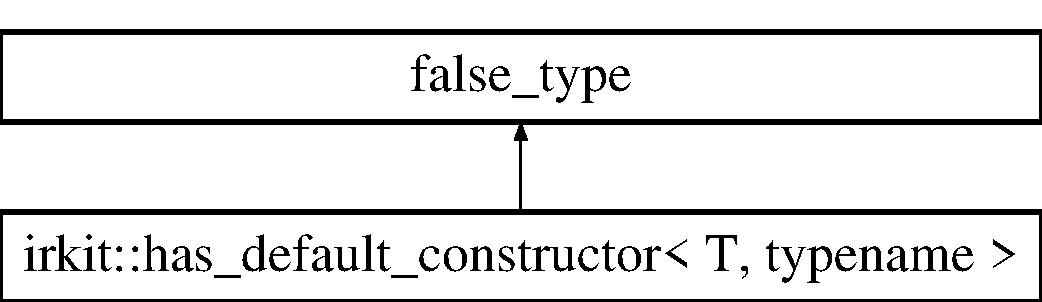
\includegraphics[height=2.000000cm]{structirkit_1_1has__default__constructor}
\end{center}
\end{figure}


The documentation for this struct was generated from the following file\+:\begin{DoxyCompactItemize}
\item 
include/irkit/\mbox{\hyperlink{heap_8hpp}{heap.\+hpp}}\end{DoxyCompactItemize}

\hypertarget{structirkit_1_1has__default__constructor_3_01T_00_01void__t_3_01decltype_07std_1_1declval_3_01T_01_6_01_4_07_08_08_4_01_4}{}\section{irkit\+:\+:has\+\_\+default\+\_\+constructor$<$ T, void\+\_\+t$<$ decltype(std\+:\+:declval$<$ T \& $>$())$>$ $>$ Struct Template Reference}
\label{structirkit_1_1has__default__constructor_3_01T_00_01void__t_3_01decltype_07std_1_1declval_3_01T_01_6_01_4_07_08_08_4_01_4}\index{irkit\+::has\+\_\+default\+\_\+constructor$<$ T, void\+\_\+t$<$ decltype(std\+::declval$<$ T \& $>$())$>$ $>$@{irkit\+::has\+\_\+default\+\_\+constructor$<$ T, void\+\_\+t$<$ decltype(std\+::declval$<$ T \& $>$())$>$ $>$}}


{\ttfamily \#include $<$heap.\+hpp$>$}

Inheritance diagram for irkit\+:\+:has\+\_\+default\+\_\+constructor$<$ T, void\+\_\+t$<$ decltype(std\+:\+:declval$<$ T \& $>$())$>$ $>$\+:\begin{figure}[H]
\begin{center}
\leavevmode
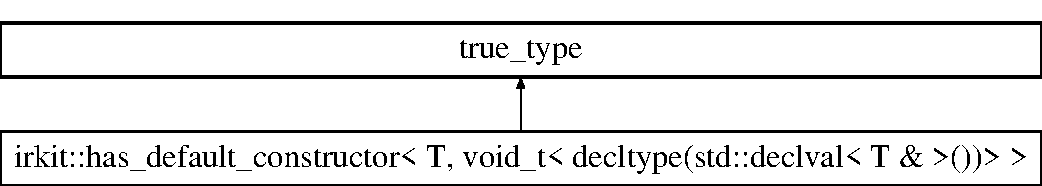
\includegraphics[height=2.000000cm]{structirkit_1_1has__default__constructor_3_01T_00_01void__t_3_01decltype_07std_1_1declval_3_01T_01_6_01_4_07_08_08_4_01_4}
\end{center}
\end{figure}


The documentation for this struct was generated from the following file\+:\begin{DoxyCompactItemize}
\item 
include/irkit/\mbox{\hyperlink{heap_8hpp}{heap.\+hpp}}\end{DoxyCompactItemize}

\hypertarget{structbloodhound_1_1query_1_1has__iterator}{}\section{bloodhound\+:\+:query\+:\+:has\+\_\+iterator$<$ T, typename $>$ Struct Template Reference}
\label{structbloodhound_1_1query_1_1has__iterator}\index{bloodhound\+::query\+::has\+\_\+iterator$<$ T, typename $>$@{bloodhound\+::query\+::has\+\_\+iterator$<$ T, typename $>$}}


{\ttfamily \#include $<$query.\+hpp$>$}

Inheritance diagram for bloodhound\+:\+:query\+:\+:has\+\_\+iterator$<$ T, typename $>$\+:\begin{figure}[H]
\begin{center}
\leavevmode
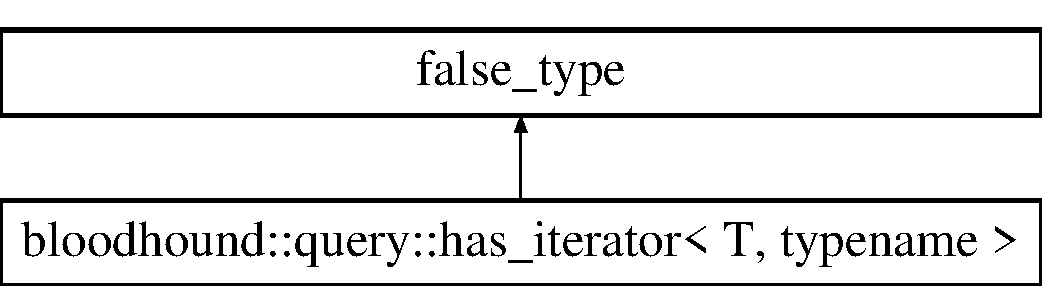
\includegraphics[height=2.000000cm]{structbloodhound_1_1query_1_1has__iterator}
\end{center}
\end{figure}


The documentation for this struct was generated from the following file\+:\begin{DoxyCompactItemize}
\item 
include/\mbox{\hyperlink{query_8hpp}{query.\+hpp}}\end{DoxyCompactItemize}

\hypertarget{structbloodhound_1_1query_1_1has__iterator_3_01T_00_01void__t_3_01typename_01T_1_1iterator_01_4_01_4}{}\section{bloodhound\+:\+:query\+:\+:has\+\_\+iterator$<$ T, void\+\_\+t$<$ typename T\+:\+:iterator $>$ $>$ Struct Template Reference}
\label{structbloodhound_1_1query_1_1has__iterator_3_01T_00_01void__t_3_01typename_01T_1_1iterator_01_4_01_4}\index{bloodhound\+::query\+::has\+\_\+iterator$<$ T, void\+\_\+t$<$ typename T\+::iterator $>$ $>$@{bloodhound\+::query\+::has\+\_\+iterator$<$ T, void\+\_\+t$<$ typename T\+::iterator $>$ $>$}}


{\ttfamily \#include $<$query.\+hpp$>$}

Inheritance diagram for bloodhound\+:\+:query\+:\+:has\+\_\+iterator$<$ T, void\+\_\+t$<$ typename T\+:\+:iterator $>$ $>$\+:\begin{figure}[H]
\begin{center}
\leavevmode
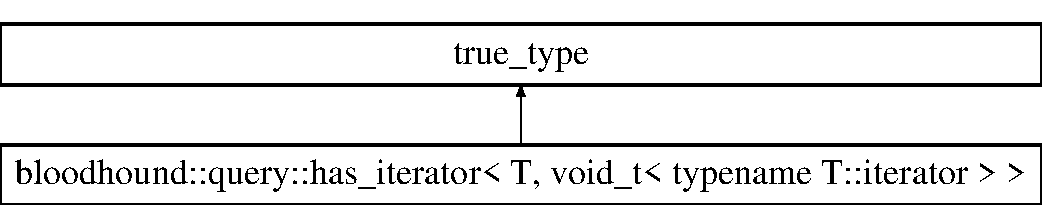
\includegraphics[height=2.000000cm]{structbloodhound_1_1query_1_1has__iterator_3_01T_00_01void__t_3_01typename_01T_1_1iterator_01_4_01_4}
\end{center}
\end{figure}


The documentation for this struct was generated from the following file\+:\begin{DoxyCompactItemize}
\item 
include/\mbox{\hyperlink{query_8hpp}{query.\+hpp}}\end{DoxyCompactItemize}

\hypertarget{structbloodhound_1_1query_1_1has__posting__iterator}{}\section{bloodhound\+:\+:query\+:\+:has\+\_\+posting\+\_\+iterator$<$ T, typename $>$ Struct Template Reference}
\label{structbloodhound_1_1query_1_1has__posting__iterator}\index{bloodhound\+::query\+::has\+\_\+posting\+\_\+iterator$<$ T, typename $>$@{bloodhound\+::query\+::has\+\_\+posting\+\_\+iterator$<$ T, typename $>$}}


{\ttfamily \#include $<$query.\+hpp$>$}

Inheritance diagram for bloodhound\+:\+:query\+:\+:has\+\_\+posting\+\_\+iterator$<$ T, typename $>$\+:\begin{figure}[H]
\begin{center}
\leavevmode
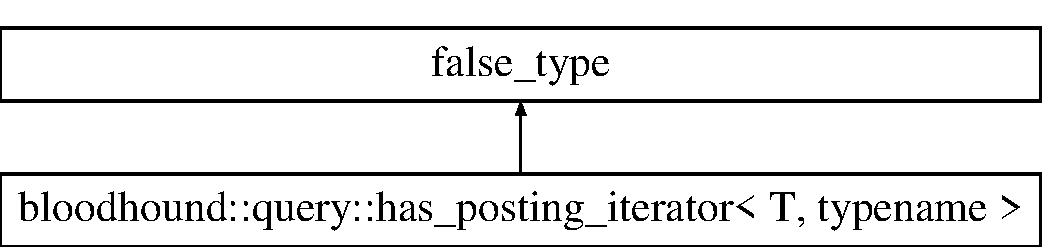
\includegraphics[height=2.000000cm]{structbloodhound_1_1query_1_1has__posting__iterator}
\end{center}
\end{figure}


The documentation for this struct was generated from the following file\+:\begin{DoxyCompactItemize}
\item 
include/\mbox{\hyperlink{query_8hpp}{query.\+hpp}}\end{DoxyCompactItemize}

\hypertarget{structbloodhound_1_1query_1_1has__posting__iterator_3_01T_00_01std_1_1enable__if__t_3_01std_1_1i3aad327a30d60305d06d5c73680c1a38}{}\section{bloodhound\+:\+:query\+:\+:has\+\_\+posting\+\_\+iterator$<$ T, std\+:\+:enable\+\_\+if\+\_\+t$<$ std\+:\+:is\+\_\+convertible$<$ decltype(std\+:\+:declval$<$ T \& $>$().end()), typename T\+:\+:iterator $>$\+:\+:value \&\&std\+:\+:is\+\_\+convertible$<$ decltype(std\+:\+:declval$<$ T \& $>$().begin()), typename T\+:\+:iterator $>$\+:\+:value \&\&std\+:\+:is\+\_\+convertible$<$ decltype($\ast$std\+:\+:declval$<$ T \& $>$().begin()), Posting \& $>$\+:\+:value \&\&std\+:\+:is\+\_\+convertible$<$ decltype($\ast$std\+:\+:declval$<$ T \& $>$().end()), Posting \& $>$\+:\+:value $>$ $>$ Struct Template Reference}
\label{structbloodhound_1_1query_1_1has__posting__iterator_3_01T_00_01std_1_1enable__if__t_3_01std_1_1i3aad327a30d60305d06d5c73680c1a38}\index{bloodhound\+::query\+::has\+\_\+posting\+\_\+iterator$<$ T, std\+::enable\+\_\+if\+\_\+t$<$ std\+::is\+\_\+convertible$<$ decltype(std\+::declval$<$ T \& $>$().\+end()), typename T\+::iterator $>$\+::value \&\&std\+::is\+\_\+convertible$<$ decltype(std\+::declval$<$ T \& $>$().\+begin()), typename T\+::iterator $>$\+::value \&\&std\+::is\+\_\+convertible$<$ decltype($\ast$std\+::declval$<$ T \& $>$().\+begin()), Posting \& $>$\+::value \&\&std\+::is\+\_\+convertible$<$ decltype($\ast$std\+::declval$<$ T \& $>$().\+end()), Posting \& $>$\+::value $>$ $>$@{bloodhound\+::query\+::has\+\_\+posting\+\_\+iterator$<$ T, std\+::enable\+\_\+if\+\_\+t$<$ std\+::is\+\_\+convertible$<$ decltype(std\+::declval$<$ T \& $>$().\+end()), typename T\+::iterator $>$\+::value \&\&std\+::is\+\_\+convertible$<$ decltype(std\+::declval$<$ T \& $>$().\+begin()), typename T\+::iterator $>$\+::value \&\&std\+::is\+\_\+convertible$<$ decltype($\ast$std\+::declval$<$ T \& $>$().\+begin()), Posting \& $>$\+::value \&\&std\+::is\+\_\+convertible$<$ decltype($\ast$std\+::declval$<$ T \& $>$().\+end()), Posting \& $>$\+::value $>$ $>$}}


{\ttfamily \#include $<$query.\+hpp$>$}

Inheritance diagram for bloodhound\+:\+:query\+:\+:has\+\_\+posting\+\_\+iterator$<$ T, std\+:\+:enable\+\_\+if\+\_\+t$<$ std\+:\+:is\+\_\+convertible$<$ decltype(std\+:\+:declval$<$ T \& $>$().end()), typename T\+:\+:iterator $>$\+:\+:value \&\&std\+:\+:is\+\_\+convertible$<$ decltype(std\+:\+:declval$<$ T \& $>$().begin()), typename T\+:\+:iterator $>$\+:\+:value \&\&std\+:\+:is\+\_\+convertible$<$ decltype($\ast$std\+:\+:declval$<$ T \& $>$().begin()), Posting \& $>$\+:\+:value \&\&std\+:\+:is\+\_\+convertible$<$ decltype($\ast$std\+:\+:declval$<$ T \& $>$().end()), Posting \& $>$\+:\+:value $>$ $>$\+:\begin{figure}[H]
\begin{center}
\leavevmode
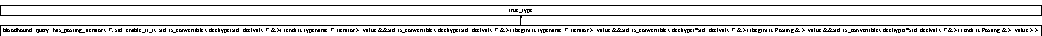
\includegraphics[height=0.480069cm]{structbloodhound_1_1query_1_1has__posting__iterator_3_01T_00_01std_1_1enable__if__t_3_01std_1_1i3aad327a30d60305d06d5c73680c1a38}
\end{center}
\end{figure}


The documentation for this struct was generated from the following file\+:\begin{DoxyCompactItemize}
\item 
include/\mbox{\hyperlink{query_8hpp}{query.\+hpp}}\end{DoxyCompactItemize}

\hypertarget{structstd_1_1hash_3_01bloodhound_1_1Doc_01_4}{}\section{std\+:\+:hash$<$ bloodhound\+:\+:Doc $>$ Struct Template Reference}
\label{structstd_1_1hash_3_01bloodhound_1_1Doc_01_4}\index{std\+::hash$<$ bloodhound\+::\+Doc $>$@{std\+::hash$<$ bloodhound\+::\+Doc $>$}}


{\ttfamily \#include $<$index.\+hpp$>$}

\subsection*{Public Member Functions}
\begin{DoxyCompactItemize}
\item 
std\+::size\+\_\+t \mbox{\hyperlink{structstd_1_1hash_3_01bloodhound_1_1Doc_01_4_a3f89deb7b2548010c7f3b63afc9d7fa4}{operator()}} (\mbox{\hyperlink{structbloodhound_1_1Doc}{bloodhound\+::\+Doc}} const \&t) const noexcept
\end{DoxyCompactItemize}


\subsection{Member Function Documentation}
\mbox{\Hypertarget{structstd_1_1hash_3_01bloodhound_1_1Doc_01_4_a3f89deb7b2548010c7f3b63afc9d7fa4}\label{structstd_1_1hash_3_01bloodhound_1_1Doc_01_4_a3f89deb7b2548010c7f3b63afc9d7fa4}} 
\index{std\+::hash$<$ bloodhound\+::\+Doc $>$@{std\+::hash$<$ bloodhound\+::\+Doc $>$}!operator()@{operator()}}
\index{operator()@{operator()}!std\+::hash$<$ bloodhound\+::\+Doc $>$@{std\+::hash$<$ bloodhound\+::\+Doc $>$}}
\subsubsection{\texorpdfstring{operator()()}{operator()()}}
{\footnotesize\ttfamily std\+::size\+\_\+t std\+::hash$<$ \mbox{\hyperlink{structbloodhound_1_1Doc}{bloodhound\+::\+Doc}} $>$\+::operator() (\begin{DoxyParamCaption}\item[{\mbox{\hyperlink{structbloodhound_1_1Doc}{bloodhound\+::\+Doc}} const \&}]{t }\end{DoxyParamCaption}) const\hspace{0.3cm}{\ttfamily [inline]}, {\ttfamily [noexcept]}}



The documentation for this struct was generated from the following file\+:\begin{DoxyCompactItemize}
\item 
include/\mbox{\hyperlink{index_8hpp}{index.\+hpp}}\end{DoxyCompactItemize}

\hypertarget{structstd_1_1hash_3_01bloodhound_1_1Score_01_4}{}\section{std\+:\+:hash$<$ bloodhound\+:\+:Score $>$ Struct Template Reference}
\label{structstd_1_1hash_3_01bloodhound_1_1Score_01_4}\index{std\+::hash$<$ bloodhound\+::\+Score $>$@{std\+::hash$<$ bloodhound\+::\+Score $>$}}


{\ttfamily \#include $<$index.\+hpp$>$}

\subsection*{Public Member Functions}
\begin{DoxyCompactItemize}
\item 
std\+::size\+\_\+t \hyperlink{structstd_1_1hash_3_01bloodhound_1_1Score_01_4_a8e9e8081ca942b25eafe41f8f76a584b}{operator()} (\hyperlink{structbloodhound_1_1Score}{bloodhound\+::\+Score} const \&t) const noexcept
\end{DoxyCompactItemize}


\subsection{Member Function Documentation}
\mbox{\Hypertarget{structstd_1_1hash_3_01bloodhound_1_1Score_01_4_a8e9e8081ca942b25eafe41f8f76a584b}\label{structstd_1_1hash_3_01bloodhound_1_1Score_01_4_a8e9e8081ca942b25eafe41f8f76a584b}} 
\index{std\+::hash$<$ bloodhound\+::\+Score $>$@{std\+::hash$<$ bloodhound\+::\+Score $>$}!operator()@{operator()}}
\index{operator()@{operator()}!std\+::hash$<$ bloodhound\+::\+Score $>$@{std\+::hash$<$ bloodhound\+::\+Score $>$}}
\subsubsection{\texorpdfstring{operator()()}{operator()()}}
{\footnotesize\ttfamily std\+::size\+\_\+t std\+::hash$<$ \hyperlink{structbloodhound_1_1Score}{bloodhound\+::\+Score} $>$\+::operator() (\begin{DoxyParamCaption}\item[{\hyperlink{structbloodhound_1_1Score}{bloodhound\+::\+Score} const \&}]{t }\end{DoxyParamCaption}) const\hspace{0.3cm}{\ttfamily [inline]}, {\ttfamily [noexcept]}}



The documentation for this struct was generated from the following file\+:\begin{DoxyCompactItemize}
\item 
include/\hyperlink{index_8hpp}{index.\+hpp}\end{DoxyCompactItemize}

\hypertarget{structstd_1_1hash_3_01bloodhound_1_1TermId_01_4}{}\section{std\+:\+:hash$<$ bloodhound\+:\+:Term\+Id $>$ Struct Template Reference}
\label{structstd_1_1hash_3_01bloodhound_1_1TermId_01_4}\index{std\+::hash$<$ bloodhound\+::\+Term\+Id $>$@{std\+::hash$<$ bloodhound\+::\+Term\+Id $>$}}


{\ttfamily \#include $<$index.\+hpp$>$}

\subsection*{Public Member Functions}
\begin{DoxyCompactItemize}
\item 
std\+::size\+\_\+t \mbox{\hyperlink{structstd_1_1hash_3_01bloodhound_1_1TermId_01_4_a7318bf08949737e1fb9dff3444fc77a1}{operator()}} (\mbox{\hyperlink{structbloodhound_1_1TermId}{bloodhound\+::\+Term\+Id}} const \&t) const noexcept
\end{DoxyCompactItemize}


\subsection{Member Function Documentation}
\mbox{\Hypertarget{structstd_1_1hash_3_01bloodhound_1_1TermId_01_4_a7318bf08949737e1fb9dff3444fc77a1}\label{structstd_1_1hash_3_01bloodhound_1_1TermId_01_4_a7318bf08949737e1fb9dff3444fc77a1}} 
\index{std\+::hash$<$ bloodhound\+::\+Term\+Id $>$@{std\+::hash$<$ bloodhound\+::\+Term\+Id $>$}!operator()@{operator()}}
\index{operator()@{operator()}!std\+::hash$<$ bloodhound\+::\+Term\+Id $>$@{std\+::hash$<$ bloodhound\+::\+Term\+Id $>$}}
\subsubsection{\texorpdfstring{operator()()}{operator()()}}
{\footnotesize\ttfamily std\+::size\+\_\+t std\+::hash$<$ \mbox{\hyperlink{structbloodhound_1_1TermId}{bloodhound\+::\+Term\+Id}} $>$\+::operator() (\begin{DoxyParamCaption}\item[{\mbox{\hyperlink{structbloodhound_1_1TermId}{bloodhound\+::\+Term\+Id}} const \&}]{t }\end{DoxyParamCaption}) const\hspace{0.3cm}{\ttfamily [inline]}, {\ttfamily [noexcept]}}



The documentation for this struct was generated from the following file\+:\begin{DoxyCompactItemize}
\item 
include/\mbox{\hyperlink{index_8hpp}{index.\+hpp}}\end{DoxyCompactItemize}

\hypertarget{classirkit_1_1Heap}{}\section{irkit\+:\+:Heap$<$ Key, Value, Compare, Mapping $>$ Class Template Reference}
\label{classirkit_1_1Heap}\index{irkit\+::\+Heap$<$ Key, Value, Compare, Mapping $>$@{irkit\+::\+Heap$<$ Key, Value, Compare, Mapping $>$}}


{\ttfamily \#include $<$heap.\+hpp$>$}

\subsection*{Public Member Functions}
\begin{DoxyCompactItemize}
\item 
\mbox{\hyperlink{classirkit_1_1Heap_ac262b1efe6564321f3f8476dc8665eaf}{Heap}} (std\+::size\+\_\+t capacity=0)
\item 
std\+::size\+\_\+t \mbox{\hyperlink{classirkit_1_1Heap_acc53589d12325834624aa08573139227}{size}} () const
\item 
bool \mbox{\hyperlink{classirkit_1_1Heap_abb96822afb46391c107efef35e79256b}{empty}} () const
\item 
\mbox{\hyperlink{structirkit_1_1Entry}{Entry}}$<$ Key, Value $>$ \mbox{\hyperlink{classirkit_1_1Heap_aa14c398611006aa94e2fe24be3cf34ec}{top}} () const
\begin{DoxyCompactList}\small\item\em Returns a copy of the top element; does not modify the heap. \end{DoxyCompactList}\item 
void \mbox{\hyperlink{classirkit_1_1Heap_a8e2dfbd02e7411fe97281b5e7d19f12c}{push}} (Key key, Value value)
\begin{DoxyCompactList}\small\item\em Adds a new element to the heap. \end{DoxyCompactList}\item 
void \mbox{\hyperlink{classirkit_1_1Heap_ae4652d2601229e4de97f0321adf5f3c6}{push\+\_\+with\+\_\+limit}} (Key key, Value value, std\+::size\+\_\+t limit)
\item 
\mbox{\hyperlink{structirkit_1_1Entry}{Entry}}$<$ Key, Value $>$ \mbox{\hyperlink{classirkit_1_1Heap_aa94f791b5b26659cc41a39fd58d138e4}{pop\+\_\+push}} (Key key, Value value)
\begin{DoxyCompactList}\small\item\em Replaces the top element with a given value and returns the former. \end{DoxyCompactList}\item 
\mbox{\hyperlink{structirkit_1_1Entry}{Entry}}$<$ Key, Value $>$ \mbox{\hyperlink{classirkit_1_1Heap_afd4759dce1fe72d513e4b8e7766ec94e}{pop}} ()
\begin{DoxyCompactList}\small\item\em Returns the top element and removes it from the heap. \end{DoxyCompactList}\item 
void \mbox{\hyperlink{classirkit_1_1Heap_a0da9e0bc583dadad14b10d285e7a8925}{remove\+\_\+value}} (Value value)
\item 
std\+::vector$<$ \mbox{\hyperlink{structirkit_1_1Entry}{Entry}}$<$ Key, Value $>$ $>$\+::iterator \mbox{\hyperlink{classirkit_1_1Heap_af996708917bb42b8cc660988c5c5ed62}{begin}} ()
\item 
std\+::vector$<$ \mbox{\hyperlink{structirkit_1_1Entry}{Entry}}$<$ Key, Value $>$ $>$\+::iterator \mbox{\hyperlink{classirkit_1_1Heap_a8451f5ab1ccb727e7964ce94e5ae3b6c}{end}} ()
\item 
void \mbox{\hyperlink{classirkit_1_1Heap_a06373b7aa5262ffc4efe381042e8cb50}{clear}} ()
\item 
Key \mbox{\hyperlink{classirkit_1_1Heap_a2fffaaf281662d57d13dcc1b0618dc0d}{key\+\_\+or}} (Value value, Key def)
\end{DoxyCompactItemize}


\subsection{Detailed Description}
\subsubsection*{template$<$class Key, class Value, class Compare = std\+::less$<$\+Key$>$, class Mapping = Empty\+Mapping$>$\newline
class irkit\+::\+Heap$<$ Key, Value, Compare, Mapping $>$}

A vector-\/based heap priority queue; a min-\/heap by default.

This implementation provides an implementation of an atomic pull-\/push operation, which is faster than a pull followed by push. Additionally, it forces you to always indicate the key and the value; it makes it easier to declare heaps without a need to create separate structures sorted by the key alone\+: all the heavy lifting is implemented within the \mbox{\hyperlink{structirkit_1_1Entry}{Entry}} type.


\begin{DoxyTemplParams}{Template Parameters}
{\em Key} & the type of the key \\
\hline
{\em Value} & the type of the value \\
\hline
{\em Compare} & a compare type providing a weak ordering \\
\hline
{\em Mapping} & a type of mapping between keys and their position; empty by default; if empty, $\ast$\+\_\+by\+\_\+key() operations are unavailable \\
\hline
\end{DoxyTemplParams}


\subsection{Constructor \& Destructor Documentation}
\mbox{\Hypertarget{classirkit_1_1Heap_ac262b1efe6564321f3f8476dc8665eaf}\label{classirkit_1_1Heap_ac262b1efe6564321f3f8476dc8665eaf}} 
\index{irkit\+::\+Heap@{irkit\+::\+Heap}!Heap@{Heap}}
\index{Heap@{Heap}!irkit\+::\+Heap@{irkit\+::\+Heap}}
\subsubsection{\texorpdfstring{Heap()}{Heap()}}
{\footnotesize\ttfamily template$<$class Key, class Value, class Compare = std\+::less$<$\+Key$>$, class Mapping = Empty\+Mapping$>$ \\
\mbox{\hyperlink{classirkit_1_1Heap}{irkit\+::\+Heap}}$<$ Key, Value, Compare, Mapping $>$\+::\mbox{\hyperlink{classirkit_1_1Heap}{Heap}} (\begin{DoxyParamCaption}\item[{std\+::size\+\_\+t}]{capacity = {\ttfamily 0} }\end{DoxyParamCaption})\hspace{0.3cm}{\ttfamily [inline]}}

\mbox{\hyperlink{classirkit_1_1Heap}{Heap}} constructor.


\begin{DoxyParams}{Parameters}
{\em capacity} & the initial capacity of the internal vector; use whenever the (max) size is known beforehand \\
\hline
\end{DoxyParams}


\subsection{Member Function Documentation}
\mbox{\Hypertarget{classirkit_1_1Heap_af996708917bb42b8cc660988c5c5ed62}\label{classirkit_1_1Heap_af996708917bb42b8cc660988c5c5ed62}} 
\index{irkit\+::\+Heap@{irkit\+::\+Heap}!begin@{begin}}
\index{begin@{begin}!irkit\+::\+Heap@{irkit\+::\+Heap}}
\subsubsection{\texorpdfstring{begin()}{begin()}}
{\footnotesize\ttfamily template$<$class Key, class Value, class Compare = std\+::less$<$\+Key$>$, class Mapping = Empty\+Mapping$>$ \\
std\+::vector$<$\mbox{\hyperlink{structirkit_1_1Entry}{Entry}}$<$Key, Value$>$ $>$\+::iterator \mbox{\hyperlink{classirkit_1_1Heap}{irkit\+::\+Heap}}$<$ Key, Value, Compare, Mapping $>$\+::begin (\begin{DoxyParamCaption}{ }\end{DoxyParamCaption})\hspace{0.3cm}{\ttfamily [inline]}}

\mbox{\Hypertarget{classirkit_1_1Heap_a06373b7aa5262ffc4efe381042e8cb50}\label{classirkit_1_1Heap_a06373b7aa5262ffc4efe381042e8cb50}} 
\index{irkit\+::\+Heap@{irkit\+::\+Heap}!clear@{clear}}
\index{clear@{clear}!irkit\+::\+Heap@{irkit\+::\+Heap}}
\subsubsection{\texorpdfstring{clear()}{clear()}}
{\footnotesize\ttfamily template$<$class Key, class Value, class Compare = std\+::less$<$\+Key$>$, class Mapping = Empty\+Mapping$>$ \\
void \mbox{\hyperlink{classirkit_1_1Heap}{irkit\+::\+Heap}}$<$ Key, Value, Compare, Mapping $>$\+::clear (\begin{DoxyParamCaption}{ }\end{DoxyParamCaption})\hspace{0.3cm}{\ttfamily [inline]}}

\mbox{\Hypertarget{classirkit_1_1Heap_abb96822afb46391c107efef35e79256b}\label{classirkit_1_1Heap_abb96822afb46391c107efef35e79256b}} 
\index{irkit\+::\+Heap@{irkit\+::\+Heap}!empty@{empty}}
\index{empty@{empty}!irkit\+::\+Heap@{irkit\+::\+Heap}}
\subsubsection{\texorpdfstring{empty()}{empty()}}
{\footnotesize\ttfamily template$<$class Key, class Value, class Compare = std\+::less$<$\+Key$>$, class Mapping = Empty\+Mapping$>$ \\
bool \mbox{\hyperlink{classirkit_1_1Heap}{irkit\+::\+Heap}}$<$ Key, Value, Compare, Mapping $>$\+::empty (\begin{DoxyParamCaption}{ }\end{DoxyParamCaption}) const\hspace{0.3cm}{\ttfamily [inline]}}

\mbox{\Hypertarget{classirkit_1_1Heap_a8451f5ab1ccb727e7964ce94e5ae3b6c}\label{classirkit_1_1Heap_a8451f5ab1ccb727e7964ce94e5ae3b6c}} 
\index{irkit\+::\+Heap@{irkit\+::\+Heap}!end@{end}}
\index{end@{end}!irkit\+::\+Heap@{irkit\+::\+Heap}}
\subsubsection{\texorpdfstring{end()}{end()}}
{\footnotesize\ttfamily template$<$class Key, class Value, class Compare = std\+::less$<$\+Key$>$, class Mapping = Empty\+Mapping$>$ \\
std\+::vector$<$\mbox{\hyperlink{structirkit_1_1Entry}{Entry}}$<$Key, Value$>$ $>$\+::iterator \mbox{\hyperlink{classirkit_1_1Heap}{irkit\+::\+Heap}}$<$ Key, Value, Compare, Mapping $>$\+::end (\begin{DoxyParamCaption}{ }\end{DoxyParamCaption})\hspace{0.3cm}{\ttfamily [inline]}}

\mbox{\Hypertarget{classirkit_1_1Heap_a2fffaaf281662d57d13dcc1b0618dc0d}\label{classirkit_1_1Heap_a2fffaaf281662d57d13dcc1b0618dc0d}} 
\index{irkit\+::\+Heap@{irkit\+::\+Heap}!key\+\_\+or@{key\+\_\+or}}
\index{key\+\_\+or@{key\+\_\+or}!irkit\+::\+Heap@{irkit\+::\+Heap}}
\subsubsection{\texorpdfstring{key\+\_\+or()}{key\_or()}}
{\footnotesize\ttfamily template$<$class Key, class Value, class Compare = std\+::less$<$\+Key$>$, class Mapping = Empty\+Mapping$>$ \\
Key \mbox{\hyperlink{classirkit_1_1Heap}{irkit\+::\+Heap}}$<$ Key, Value, Compare, Mapping $>$\+::key\+\_\+or (\begin{DoxyParamCaption}\item[{Value}]{value,  }\item[{Key}]{def }\end{DoxyParamCaption})\hspace{0.3cm}{\ttfamily [inline]}}

\mbox{\Hypertarget{classirkit_1_1Heap_afd4759dce1fe72d513e4b8e7766ec94e}\label{classirkit_1_1Heap_afd4759dce1fe72d513e4b8e7766ec94e}} 
\index{irkit\+::\+Heap@{irkit\+::\+Heap}!pop@{pop}}
\index{pop@{pop}!irkit\+::\+Heap@{irkit\+::\+Heap}}
\subsubsection{\texorpdfstring{pop()}{pop()}}
{\footnotesize\ttfamily template$<$class Key, class Value, class Compare = std\+::less$<$\+Key$>$, class Mapping = Empty\+Mapping$>$ \\
\mbox{\hyperlink{structirkit_1_1Entry}{Entry}}$<$Key, Value$>$ \mbox{\hyperlink{classirkit_1_1Heap}{irkit\+::\+Heap}}$<$ Key, Value, Compare, Mapping $>$\+::pop (\begin{DoxyParamCaption}{ }\end{DoxyParamCaption})\hspace{0.3cm}{\ttfamily [inline]}}



Returns the top element and removes it from the heap. 

\mbox{\Hypertarget{classirkit_1_1Heap_aa94f791b5b26659cc41a39fd58d138e4}\label{classirkit_1_1Heap_aa94f791b5b26659cc41a39fd58d138e4}} 
\index{irkit\+::\+Heap@{irkit\+::\+Heap}!pop\+\_\+push@{pop\+\_\+push}}
\index{pop\+\_\+push@{pop\+\_\+push}!irkit\+::\+Heap@{irkit\+::\+Heap}}
\subsubsection{\texorpdfstring{pop\+\_\+push()}{pop\_push()}}
{\footnotesize\ttfamily template$<$class Key, class Value, class Compare = std\+::less$<$\+Key$>$, class Mapping = Empty\+Mapping$>$ \\
\mbox{\hyperlink{structirkit_1_1Entry}{Entry}}$<$Key, Value$>$ \mbox{\hyperlink{classirkit_1_1Heap}{irkit\+::\+Heap}}$<$ Key, Value, Compare, Mapping $>$\+::pop\+\_\+push (\begin{DoxyParamCaption}\item[{Key}]{key,  }\item[{Value}]{value }\end{DoxyParamCaption})\hspace{0.3cm}{\ttfamily [inline]}}



Replaces the top element with a given value and returns the former. 

\mbox{\Hypertarget{classirkit_1_1Heap_a8e2dfbd02e7411fe97281b5e7d19f12c}\label{classirkit_1_1Heap_a8e2dfbd02e7411fe97281b5e7d19f12c}} 
\index{irkit\+::\+Heap@{irkit\+::\+Heap}!push@{push}}
\index{push@{push}!irkit\+::\+Heap@{irkit\+::\+Heap}}
\subsubsection{\texorpdfstring{push()}{push()}}
{\footnotesize\ttfamily template$<$class Key, class Value, class Compare = std\+::less$<$\+Key$>$, class Mapping = Empty\+Mapping$>$ \\
void \mbox{\hyperlink{classirkit_1_1Heap}{irkit\+::\+Heap}}$<$ Key, Value, Compare, Mapping $>$\+::push (\begin{DoxyParamCaption}\item[{Key}]{key,  }\item[{Value}]{value }\end{DoxyParamCaption})\hspace{0.3cm}{\ttfamily [inline]}}



Adds a new element to the heap. 

\mbox{\Hypertarget{classirkit_1_1Heap_ae4652d2601229e4de97f0321adf5f3c6}\label{classirkit_1_1Heap_ae4652d2601229e4de97f0321adf5f3c6}} 
\index{irkit\+::\+Heap@{irkit\+::\+Heap}!push\+\_\+with\+\_\+limit@{push\+\_\+with\+\_\+limit}}
\index{push\+\_\+with\+\_\+limit@{push\+\_\+with\+\_\+limit}!irkit\+::\+Heap@{irkit\+::\+Heap}}
\subsubsection{\texorpdfstring{push\+\_\+with\+\_\+limit()}{push\_with\_limit()}}
{\footnotesize\ttfamily template$<$class Key, class Value, class Compare = std\+::less$<$\+Key$>$, class Mapping = Empty\+Mapping$>$ \\
void \mbox{\hyperlink{classirkit_1_1Heap}{irkit\+::\+Heap}}$<$ Key, Value, Compare, Mapping $>$\+::push\+\_\+with\+\_\+limit (\begin{DoxyParamCaption}\item[{Key}]{key,  }\item[{Value}]{value,  }\item[{std\+::size\+\_\+t}]{limit }\end{DoxyParamCaption})\hspace{0.3cm}{\ttfamily [inline]}}

Adds a new element to the heap unless the capacity limit is reached; in case of an overflow, the new element replaces the top element only if it is not smaller (for min-\/heap) than the current top key. \mbox{\Hypertarget{classirkit_1_1Heap_a0da9e0bc583dadad14b10d285e7a8925}\label{classirkit_1_1Heap_a0da9e0bc583dadad14b10d285e7a8925}} 
\index{irkit\+::\+Heap@{irkit\+::\+Heap}!remove\+\_\+value@{remove\+\_\+value}}
\index{remove\+\_\+value@{remove\+\_\+value}!irkit\+::\+Heap@{irkit\+::\+Heap}}
\subsubsection{\texorpdfstring{remove\+\_\+value()}{remove\_value()}}
{\footnotesize\ttfamily template$<$class Key, class Value, class Compare = std\+::less$<$\+Key$>$, class Mapping = Empty\+Mapping$>$ \\
void \mbox{\hyperlink{classirkit_1_1Heap}{irkit\+::\+Heap}}$<$ Key, Value, Compare, Mapping $>$\+::remove\+\_\+value (\begin{DoxyParamCaption}\item[{Value}]{value }\end{DoxyParamCaption})\hspace{0.3cm}{\ttfamily [inline]}}

\mbox{\Hypertarget{classirkit_1_1Heap_acc53589d12325834624aa08573139227}\label{classirkit_1_1Heap_acc53589d12325834624aa08573139227}} 
\index{irkit\+::\+Heap@{irkit\+::\+Heap}!size@{size}}
\index{size@{size}!irkit\+::\+Heap@{irkit\+::\+Heap}}
\subsubsection{\texorpdfstring{size()}{size()}}
{\footnotesize\ttfamily template$<$class Key, class Value, class Compare = std\+::less$<$\+Key$>$, class Mapping = Empty\+Mapping$>$ \\
std\+::size\+\_\+t \mbox{\hyperlink{classirkit_1_1Heap}{irkit\+::\+Heap}}$<$ Key, Value, Compare, Mapping $>$\+::size (\begin{DoxyParamCaption}{ }\end{DoxyParamCaption}) const\hspace{0.3cm}{\ttfamily [inline]}}

\mbox{\Hypertarget{classirkit_1_1Heap_aa14c398611006aa94e2fe24be3cf34ec}\label{classirkit_1_1Heap_aa14c398611006aa94e2fe24be3cf34ec}} 
\index{irkit\+::\+Heap@{irkit\+::\+Heap}!top@{top}}
\index{top@{top}!irkit\+::\+Heap@{irkit\+::\+Heap}}
\subsubsection{\texorpdfstring{top()}{top()}}
{\footnotesize\ttfamily template$<$class Key, class Value, class Compare = std\+::less$<$\+Key$>$, class Mapping = Empty\+Mapping$>$ \\
\mbox{\hyperlink{structirkit_1_1Entry}{Entry}}$<$Key, Value$>$ \mbox{\hyperlink{classirkit_1_1Heap}{irkit\+::\+Heap}}$<$ Key, Value, Compare, Mapping $>$\+::top (\begin{DoxyParamCaption}{ }\end{DoxyParamCaption}) const\hspace{0.3cm}{\ttfamily [inline]}}



Returns a copy of the top element; does not modify the heap. 



The documentation for this class was generated from the following file\+:\begin{DoxyCompactItemize}
\item 
include/irkit/\mbox{\hyperlink{heap_8hpp}{heap.\+hpp}}\end{DoxyCompactItemize}

\hypertarget{structirkit_1_1IdWeight}{}\section{irkit\+:\+:Id\+Weight Struct Reference}
\label{structirkit_1_1IdWeight}\index{irkit\+::\+Id\+Weight@{irkit\+::\+Id\+Weight}}


{\ttfamily \#include $<$taat.\+hpp$>$}



The documentation for this struct was generated from the following file\+:\begin{DoxyCompactItemize}
\item 
include/irkit/\hyperlink{taat_8hpp}{taat.\+hpp}\end{DoxyCompactItemize}

\hypertarget{classirkit_1_1Index}{}\section{irkit\+:\+:Index$<$ Doc, Term, Term\+Id, Freq $>$ Class Template Reference}
\label{classirkit_1_1Index}\index{irkit\+::\+Index$<$ Doc, Term, Term\+Id, Freq $>$@{irkit\+::\+Index$<$ Doc, Term, Term\+Id, Freq $>$}}


{\ttfamily \#include $<$index.\+hpp$>$}

\subsection*{Public Member Functions}
\begin{DoxyCompactItemize}
\item 
\hyperlink{classirkit_1_1Index_a42309f5d0a921f9663fa3980a3122839}{Index} (std\+::vector$<$ Term $>$ terms, std\+::vector$<$ Freq $>$ term\+\_\+dfs, std\+::vector$<$ char $>$ doc\+\_\+ids, std\+::vector$<$ std\+::size\+\_\+t $>$ doc\+\_\+ids\+\_\+off, std\+::vector$<$ char $>$ doc\+\_\+counts, std\+::vector$<$ std\+::size\+\_\+t $>$ doc\+\_\+counts\+\_\+off, std\+::vector$<$ std\+::string $>$ \hyperlink{classirkit_1_1Index_a632caff9525484c5d453d016c5cb586e}{titles})
\item 
\hyperlink{classirkit_1_1Index_ac5cba6928ec1e67be4f59089b3a51b89}{Index} (fs\+::path dir, bool in\+\_\+memory=true, bool skip\+\_\+term\+\_\+map=false)
\item 
void \hyperlink{classirkit_1_1Index_af8a4dd64292b2b7f7359ef1e62d75147}{load\+\_\+term\+\_\+dfs} (fs\+::path term\+\_\+df\+\_\+file)
\item 
void \hyperlink{classirkit_1_1Index_acd33c3a279e165a71594843d70e281f1}{load\+\_\+titles} (fs\+::path titles\+\_\+file)
\item 
void \hyperlink{classirkit_1_1Index_a2071c83ea3a4f128ea624fea8a24c9c9}{load\+\_\+term\+\_\+map} (fs\+::path term\+\_\+file)
\item 
void \hyperlink{classirkit_1_1Index_a1d44636a2174a740a9e648d2587254a6}{load\+\_\+offsets} (fs\+::path offset\+\_\+file, std\+::vector$<$ std\+::size\+\_\+t $>$ \&offsets)
\item 
void \hyperlink{classirkit_1_1Index_acdc1ba811044619795c2ab7eeed13abc}{load\+\_\+data} (fs\+::path data\+\_\+file, std\+::vector$<$ char $>$ \&data\+\_\+container) const
\item 
std\+::size\+\_\+t \hyperlink{classirkit_1_1Index_a47d88bb03c2c547fc159739b13871f68}{file\+\_\+size} (fs\+::path file)
\item 
std\+::vector$<$ char $>$ \hyperlink{classirkit_1_1Index_a2dfd40f97f0022b075c8aaa38d96edc7}{load\+\_\+data} (fs\+::path data\+\_\+file, std\+::size\+\_\+t start, std\+::size\+\_\+t size) const
\item 
std\+::size\+\_\+t \hyperlink{classirkit_1_1Index_a45ede4e9e43c8a813d13467d97c084a1}{collection\+\_\+size} () const
\item 
{\footnotesize template$<$class Score\+Fn  = score\+::\+Tf\+Idf$>$ }\\auto \hyperlink{classirkit_1_1Index_ada30daf417b2dc957840170d90dba798}{posting\+\_\+ranges} (const std\+::vector$<$ std\+::string $>$ \&terms, Score\+Fn score\+\_\+fn=\hyperlink{structirkit_1_1score_1_1TfIdf}{score\+::\+Tf\+Idf}\{\}) const -\/$>$ std\+::vector$<$ \hyperlink{classirkit_1_1DynamiclyScoredPostingRange}{Dynamicly\+Scored\+Posting\+Range}$<$ \hyperlink{structirkit_1_1__Posting}{\+\_\+\+Posting}$<$ Doc, \hyperlink{namespaceirkit_1_1score_ab6226695d6d5c54c84fcf2cb8e90c8b3}{score\+::score\+\_\+result\+\_\+t}$<$ Score\+Fn, Doc, Freq $>$$>$, Freq, Score\+Fn $>$$>$
\item 
{\footnotesize template$<$class Score\+Fn  = score\+::\+Tf\+Idf$>$ }\\auto \hyperlink{classirkit_1_1Index_a931de856b06aac7957f7182048e8e852}{posting\+\_\+range} (const std\+::string \&\hyperlink{classirkit_1_1Index_a62050b0a8c8556262b82a45be1ae0262}{term}, Score\+Fn score\+\_\+fn=\hyperlink{structirkit_1_1score_1_1TfIdf}{score\+::\+Tf\+Idf}\{\}) const -\/$>$ \hyperlink{classirkit_1_1DynamiclyScoredPostingRange}{Dynamicly\+Scored\+Posting\+Range}$<$ \hyperlink{structirkit_1_1__Posting}{\+\_\+\+Posting}$<$ Doc, \hyperlink{namespaceirkit_1_1score_ab6226695d6d5c54c84fcf2cb8e90c8b3}{score\+::score\+\_\+result\+\_\+t}$<$ Score\+Fn, Doc, Freq $>$$>$, Freq, Score\+Fn $>$
\item 
{\footnotesize template$<$class Score\+Fn  = score\+::\+Tf\+Idf$>$ }\\auto \hyperlink{classirkit_1_1Index_abeb1c1b2ddc660e42c5c6dad0bab4dc4}{posting\+\_\+range} (Term\+Id term\+\_\+id, Score\+Fn score\+\_\+fn=\hyperlink{structirkit_1_1score_1_1TfIdf}{score\+::\+Tf\+Idf}\{\}) const -\/$>$ \hyperlink{classirkit_1_1DynamiclyScoredPostingRange}{Dynamicly\+Scored\+Posting\+Range}$<$ \hyperlink{structirkit_1_1__Posting}{\+\_\+\+Posting}$<$ Doc, \hyperlink{namespaceirkit_1_1score_ab6226695d6d5c54c84fcf2cb8e90c8b3}{score\+::score\+\_\+result\+\_\+t}$<$ Score\+Fn, Doc, Freq $>$$>$, Freq, Score\+Fn $>$
\item 
std\+::string \hyperlink{classirkit_1_1Index_a6a4d5f7860e2359b89270d20302e6f0b}{title} (Doc doc\+\_\+id) const
\item 
const std\+::vector$<$ std\+::string $>$ \& \hyperlink{classirkit_1_1Index_a632caff9525484c5d453d016c5cb586e}{titles} () const
\item 
Term \hyperlink{classirkit_1_1Index_a62050b0a8c8556262b82a45be1ae0262}{term} (Term\+Id term\+\_\+id) const
\item 
std\+::size\+\_\+t \hyperlink{classirkit_1_1Index_a3051984667589401814296f54e72e32c}{term\+\_\+count} () const
\end{DoxyCompactItemize}


\subsection{Constructor \& Destructor Documentation}
\mbox{\Hypertarget{classirkit_1_1Index_a42309f5d0a921f9663fa3980a3122839}\label{classirkit_1_1Index_a42309f5d0a921f9663fa3980a3122839}} 
\index{irkit\+::\+Index@{irkit\+::\+Index}!Index@{Index}}
\index{Index@{Index}!irkit\+::\+Index@{irkit\+::\+Index}}
\subsubsection{\texorpdfstring{Index()}{Index()}\hspace{0.1cm}{\footnotesize\ttfamily [1/2]}}
{\footnotesize\ttfamily template$<$class Doc  = std\+::size\+\_\+t, class Term  = std\+::string, class Term\+Id  = std\+::size\+\_\+t, class Freq  = std\+::size\+\_\+t$>$ \\
\hyperlink{classirkit_1_1Index}{irkit\+::\+Index}$<$ Doc, Term, Term\+Id, Freq $>$\+::\hyperlink{classirkit_1_1Index}{Index} (\begin{DoxyParamCaption}\item[{std\+::vector$<$ Term $>$}]{terms,  }\item[{std\+::vector$<$ Freq $>$}]{term\+\_\+dfs,  }\item[{std\+::vector$<$ char $>$}]{doc\+\_\+ids,  }\item[{std\+::vector$<$ std\+::size\+\_\+t $>$}]{doc\+\_\+ids\+\_\+off,  }\item[{std\+::vector$<$ char $>$}]{doc\+\_\+counts,  }\item[{std\+::vector$<$ std\+::size\+\_\+t $>$}]{doc\+\_\+counts\+\_\+off,  }\item[{std\+::vector$<$ std\+::string $>$}]{titles }\end{DoxyParamCaption})\hspace{0.3cm}{\ttfamily [inline]}}

\mbox{\Hypertarget{classirkit_1_1Index_ac5cba6928ec1e67be4f59089b3a51b89}\label{classirkit_1_1Index_ac5cba6928ec1e67be4f59089b3a51b89}} 
\index{irkit\+::\+Index@{irkit\+::\+Index}!Index@{Index}}
\index{Index@{Index}!irkit\+::\+Index@{irkit\+::\+Index}}
\subsubsection{\texorpdfstring{Index()}{Index()}\hspace{0.1cm}{\footnotesize\ttfamily [2/2]}}
{\footnotesize\ttfamily template$<$class Doc  = std\+::size\+\_\+t, class Term  = std\+::string, class Term\+Id  = std\+::size\+\_\+t, class Freq  = std\+::size\+\_\+t$>$ \\
\hyperlink{classirkit_1_1Index}{irkit\+::\+Index}$<$ Doc, Term, Term\+Id, Freq $>$\+::\hyperlink{classirkit_1_1Index}{Index} (\begin{DoxyParamCaption}\item[{fs\+::path}]{dir,  }\item[{bool}]{in\+\_\+memory = {\ttfamily true},  }\item[{bool}]{skip\+\_\+term\+\_\+map = {\ttfamily false} }\end{DoxyParamCaption})\hspace{0.3cm}{\ttfamily [inline]}}



\subsection{Member Function Documentation}
\mbox{\Hypertarget{classirkit_1_1Index_a45ede4e9e43c8a813d13467d97c084a1}\label{classirkit_1_1Index_a45ede4e9e43c8a813d13467d97c084a1}} 
\index{irkit\+::\+Index@{irkit\+::\+Index}!collection\+\_\+size@{collection\+\_\+size}}
\index{collection\+\_\+size@{collection\+\_\+size}!irkit\+::\+Index@{irkit\+::\+Index}}
\subsubsection{\texorpdfstring{collection\+\_\+size()}{collection\_size()}}
{\footnotesize\ttfamily template$<$class Doc  = std\+::size\+\_\+t, class Term  = std\+::string, class Term\+Id  = std\+::size\+\_\+t, class Freq  = std\+::size\+\_\+t$>$ \\
std\+::size\+\_\+t \hyperlink{classirkit_1_1Index}{irkit\+::\+Index}$<$ Doc, Term, Term\+Id, Freq $>$\+::collection\+\_\+size (\begin{DoxyParamCaption}{ }\end{DoxyParamCaption}) const\hspace{0.3cm}{\ttfamily [inline]}}

\mbox{\Hypertarget{classirkit_1_1Index_a47d88bb03c2c547fc159739b13871f68}\label{classirkit_1_1Index_a47d88bb03c2c547fc159739b13871f68}} 
\index{irkit\+::\+Index@{irkit\+::\+Index}!file\+\_\+size@{file\+\_\+size}}
\index{file\+\_\+size@{file\+\_\+size}!irkit\+::\+Index@{irkit\+::\+Index}}
\subsubsection{\texorpdfstring{file\+\_\+size()}{file\_size()}}
{\footnotesize\ttfamily template$<$class Doc  = std\+::size\+\_\+t, class Term  = std\+::string, class Term\+Id  = std\+::size\+\_\+t, class Freq  = std\+::size\+\_\+t$>$ \\
std\+::size\+\_\+t \hyperlink{classirkit_1_1Index}{irkit\+::\+Index}$<$ Doc, Term, Term\+Id, Freq $>$\+::file\+\_\+size (\begin{DoxyParamCaption}\item[{fs\+::path}]{file }\end{DoxyParamCaption})\hspace{0.3cm}{\ttfamily [inline]}}

\mbox{\Hypertarget{classirkit_1_1Index_acdc1ba811044619795c2ab7eeed13abc}\label{classirkit_1_1Index_acdc1ba811044619795c2ab7eeed13abc}} 
\index{irkit\+::\+Index@{irkit\+::\+Index}!load\+\_\+data@{load\+\_\+data}}
\index{load\+\_\+data@{load\+\_\+data}!irkit\+::\+Index@{irkit\+::\+Index}}
\subsubsection{\texorpdfstring{load\+\_\+data()}{load\_data()}\hspace{0.1cm}{\footnotesize\ttfamily [1/2]}}
{\footnotesize\ttfamily template$<$class Doc  = std\+::size\+\_\+t, class Term  = std\+::string, class Term\+Id  = std\+::size\+\_\+t, class Freq  = std\+::size\+\_\+t$>$ \\
void \hyperlink{classirkit_1_1Index}{irkit\+::\+Index}$<$ Doc, Term, Term\+Id, Freq $>$\+::load\+\_\+data (\begin{DoxyParamCaption}\item[{fs\+::path}]{data\+\_\+file,  }\item[{std\+::vector$<$ char $>$ \&}]{data\+\_\+container }\end{DoxyParamCaption}) const\hspace{0.3cm}{\ttfamily [inline]}}

\mbox{\Hypertarget{classirkit_1_1Index_a2dfd40f97f0022b075c8aaa38d96edc7}\label{classirkit_1_1Index_a2dfd40f97f0022b075c8aaa38d96edc7}} 
\index{irkit\+::\+Index@{irkit\+::\+Index}!load\+\_\+data@{load\+\_\+data}}
\index{load\+\_\+data@{load\+\_\+data}!irkit\+::\+Index@{irkit\+::\+Index}}
\subsubsection{\texorpdfstring{load\+\_\+data()}{load\_data()}\hspace{0.1cm}{\footnotesize\ttfamily [2/2]}}
{\footnotesize\ttfamily template$<$class Doc  = std\+::size\+\_\+t, class Term  = std\+::string, class Term\+Id  = std\+::size\+\_\+t, class Freq  = std\+::size\+\_\+t$>$ \\
std\+::vector$<$char$>$ \hyperlink{classirkit_1_1Index}{irkit\+::\+Index}$<$ Doc, Term, Term\+Id, Freq $>$\+::load\+\_\+data (\begin{DoxyParamCaption}\item[{fs\+::path}]{data\+\_\+file,  }\item[{std\+::size\+\_\+t}]{start,  }\item[{std\+::size\+\_\+t}]{size }\end{DoxyParamCaption}) const\hspace{0.3cm}{\ttfamily [inline]}}

\mbox{\Hypertarget{classirkit_1_1Index_a1d44636a2174a740a9e648d2587254a6}\label{classirkit_1_1Index_a1d44636a2174a740a9e648d2587254a6}} 
\index{irkit\+::\+Index@{irkit\+::\+Index}!load\+\_\+offsets@{load\+\_\+offsets}}
\index{load\+\_\+offsets@{load\+\_\+offsets}!irkit\+::\+Index@{irkit\+::\+Index}}
\subsubsection{\texorpdfstring{load\+\_\+offsets()}{load\_offsets()}}
{\footnotesize\ttfamily template$<$class Doc  = std\+::size\+\_\+t, class Term  = std\+::string, class Term\+Id  = std\+::size\+\_\+t, class Freq  = std\+::size\+\_\+t$>$ \\
void \hyperlink{classirkit_1_1Index}{irkit\+::\+Index}$<$ Doc, Term, Term\+Id, Freq $>$\+::load\+\_\+offsets (\begin{DoxyParamCaption}\item[{fs\+::path}]{offset\+\_\+file,  }\item[{std\+::vector$<$ std\+::size\+\_\+t $>$ \&}]{offsets }\end{DoxyParamCaption})\hspace{0.3cm}{\ttfamily [inline]}}

\mbox{\Hypertarget{classirkit_1_1Index_af8a4dd64292b2b7f7359ef1e62d75147}\label{classirkit_1_1Index_af8a4dd64292b2b7f7359ef1e62d75147}} 
\index{irkit\+::\+Index@{irkit\+::\+Index}!load\+\_\+term\+\_\+dfs@{load\+\_\+term\+\_\+dfs}}
\index{load\+\_\+term\+\_\+dfs@{load\+\_\+term\+\_\+dfs}!irkit\+::\+Index@{irkit\+::\+Index}}
\subsubsection{\texorpdfstring{load\+\_\+term\+\_\+dfs()}{load\_term\_dfs()}}
{\footnotesize\ttfamily template$<$class Doc  = std\+::size\+\_\+t, class Term  = std\+::string, class Term\+Id  = std\+::size\+\_\+t, class Freq  = std\+::size\+\_\+t$>$ \\
void \hyperlink{classirkit_1_1Index}{irkit\+::\+Index}$<$ Doc, Term, Term\+Id, Freq $>$\+::load\+\_\+term\+\_\+dfs (\begin{DoxyParamCaption}\item[{fs\+::path}]{term\+\_\+df\+\_\+file }\end{DoxyParamCaption})\hspace{0.3cm}{\ttfamily [inline]}}

\mbox{\Hypertarget{classirkit_1_1Index_a2071c83ea3a4f128ea624fea8a24c9c9}\label{classirkit_1_1Index_a2071c83ea3a4f128ea624fea8a24c9c9}} 
\index{irkit\+::\+Index@{irkit\+::\+Index}!load\+\_\+term\+\_\+map@{load\+\_\+term\+\_\+map}}
\index{load\+\_\+term\+\_\+map@{load\+\_\+term\+\_\+map}!irkit\+::\+Index@{irkit\+::\+Index}}
\subsubsection{\texorpdfstring{load\+\_\+term\+\_\+map()}{load\_term\_map()}}
{\footnotesize\ttfamily template$<$class Doc  = std\+::size\+\_\+t, class Term  = std\+::string, class Term\+Id  = std\+::size\+\_\+t, class Freq  = std\+::size\+\_\+t$>$ \\
void \hyperlink{classirkit_1_1Index}{irkit\+::\+Index}$<$ Doc, Term, Term\+Id, Freq $>$\+::load\+\_\+term\+\_\+map (\begin{DoxyParamCaption}\item[{fs\+::path}]{term\+\_\+file }\end{DoxyParamCaption})\hspace{0.3cm}{\ttfamily [inline]}}

\mbox{\Hypertarget{classirkit_1_1Index_acd33c3a279e165a71594843d70e281f1}\label{classirkit_1_1Index_acd33c3a279e165a71594843d70e281f1}} 
\index{irkit\+::\+Index@{irkit\+::\+Index}!load\+\_\+titles@{load\+\_\+titles}}
\index{load\+\_\+titles@{load\+\_\+titles}!irkit\+::\+Index@{irkit\+::\+Index}}
\subsubsection{\texorpdfstring{load\+\_\+titles()}{load\_titles()}}
{\footnotesize\ttfamily template$<$class Doc  = std\+::size\+\_\+t, class Term  = std\+::string, class Term\+Id  = std\+::size\+\_\+t, class Freq  = std\+::size\+\_\+t$>$ \\
void \hyperlink{classirkit_1_1Index}{irkit\+::\+Index}$<$ Doc, Term, Term\+Id, Freq $>$\+::load\+\_\+titles (\begin{DoxyParamCaption}\item[{fs\+::path}]{titles\+\_\+file }\end{DoxyParamCaption})\hspace{0.3cm}{\ttfamily [inline]}}

\mbox{\Hypertarget{classirkit_1_1Index_a931de856b06aac7957f7182048e8e852}\label{classirkit_1_1Index_a931de856b06aac7957f7182048e8e852}} 
\index{irkit\+::\+Index@{irkit\+::\+Index}!posting\+\_\+range@{posting\+\_\+range}}
\index{posting\+\_\+range@{posting\+\_\+range}!irkit\+::\+Index@{irkit\+::\+Index}}
\subsubsection{\texorpdfstring{posting\+\_\+range()}{posting\_range()}\hspace{0.1cm}{\footnotesize\ttfamily [1/2]}}
{\footnotesize\ttfamily template$<$class Doc  = std\+::size\+\_\+t, class Term  = std\+::string, class Term\+Id  = std\+::size\+\_\+t, class Freq  = std\+::size\+\_\+t$>$ \\
template$<$class Score\+Fn  = score\+::\+Tf\+Idf$>$ \\
auto \hyperlink{classirkit_1_1Index}{irkit\+::\+Index}$<$ Doc, Term, Term\+Id, Freq $>$\+::posting\+\_\+range (\begin{DoxyParamCaption}\item[{const std\+::string \&}]{term,  }\item[{Score\+Fn}]{score\+\_\+fn = {\ttfamily \hyperlink{structirkit_1_1score_1_1TfIdf}{score\+::\+Tf\+Idf}\{\}} }\end{DoxyParamCaption}) const -\/$>$ \hyperlink{classirkit_1_1DynamiclyScoredPostingRange}{Dynamicly\+Scored\+Posting\+Range}$<$
            \hyperlink{structirkit_1_1__Posting}{\+\_\+\+Posting}$<$Doc, \hyperlink{namespaceirkit_1_1score_ab6226695d6d5c54c84fcf2cb8e90c8b3}{score\+::score\+\_\+result\+\_\+t}$<$Score\+Fn, Doc, Freq$>$$>$,
            Freq,
            Score\+Fn$>$
    \hspace{0.3cm}{\ttfamily [inline]}}

\mbox{\Hypertarget{classirkit_1_1Index_abeb1c1b2ddc660e42c5c6dad0bab4dc4}\label{classirkit_1_1Index_abeb1c1b2ddc660e42c5c6dad0bab4dc4}} 
\index{irkit\+::\+Index@{irkit\+::\+Index}!posting\+\_\+range@{posting\+\_\+range}}
\index{posting\+\_\+range@{posting\+\_\+range}!irkit\+::\+Index@{irkit\+::\+Index}}
\subsubsection{\texorpdfstring{posting\+\_\+range()}{posting\_range()}\hspace{0.1cm}{\footnotesize\ttfamily [2/2]}}
{\footnotesize\ttfamily template$<$class Doc  = std\+::size\+\_\+t, class Term  = std\+::string, class Term\+Id  = std\+::size\+\_\+t, class Freq  = std\+::size\+\_\+t$>$ \\
template$<$class Score\+Fn  = score\+::\+Tf\+Idf$>$ \\
auto \hyperlink{classirkit_1_1Index}{irkit\+::\+Index}$<$ Doc, Term, Term\+Id, Freq $>$\+::posting\+\_\+range (\begin{DoxyParamCaption}\item[{Term\+Id}]{term\+\_\+id,  }\item[{Score\+Fn}]{score\+\_\+fn = {\ttfamily \hyperlink{structirkit_1_1score_1_1TfIdf}{score\+::\+Tf\+Idf}\{\}} }\end{DoxyParamCaption}) const -\/$>$ \hyperlink{classirkit_1_1DynamiclyScoredPostingRange}{Dynamicly\+Scored\+Posting\+Range}$<$
            \hyperlink{structirkit_1_1__Posting}{\+\_\+\+Posting}$<$Doc, \hyperlink{namespaceirkit_1_1score_ab6226695d6d5c54c84fcf2cb8e90c8b3}{score\+::score\+\_\+result\+\_\+t}$<$Score\+Fn, Doc, Freq$>$$>$,
            Freq,
            Score\+Fn$>$
    \hspace{0.3cm}{\ttfamily [inline]}}

\mbox{\Hypertarget{classirkit_1_1Index_ada30daf417b2dc957840170d90dba798}\label{classirkit_1_1Index_ada30daf417b2dc957840170d90dba798}} 
\index{irkit\+::\+Index@{irkit\+::\+Index}!posting\+\_\+ranges@{posting\+\_\+ranges}}
\index{posting\+\_\+ranges@{posting\+\_\+ranges}!irkit\+::\+Index@{irkit\+::\+Index}}
\subsubsection{\texorpdfstring{posting\+\_\+ranges()}{posting\_ranges()}}
{\footnotesize\ttfamily template$<$class Doc  = std\+::size\+\_\+t, class Term  = std\+::string, class Term\+Id  = std\+::size\+\_\+t, class Freq  = std\+::size\+\_\+t$>$ \\
template$<$class Score\+Fn  = score\+::\+Tf\+Idf$>$ \\
auto \hyperlink{classirkit_1_1Index}{irkit\+::\+Index}$<$ Doc, Term, Term\+Id, Freq $>$\+::posting\+\_\+ranges (\begin{DoxyParamCaption}\item[{const std\+::vector$<$ std\+::string $>$ \&}]{terms,  }\item[{Score\+Fn}]{score\+\_\+fn = {\ttfamily \hyperlink{structirkit_1_1score_1_1TfIdf}{score\+::\+Tf\+Idf}\{\}} }\end{DoxyParamCaption}) const -\/$>$ std\+::vector$<$\hyperlink{classirkit_1_1DynamiclyScoredPostingRange}{Dynamicly\+Scored\+Posting\+Range}$<$
            \hyperlink{structirkit_1_1__Posting}{\+\_\+\+Posting}$<$Doc, \hyperlink{namespaceirkit_1_1score_ab6226695d6d5c54c84fcf2cb8e90c8b3}{score\+::score\+\_\+result\+\_\+t}$<$Score\+Fn, Doc, Freq$>$$>$,
            Freq,
            Score\+Fn$>$$>$
    \hspace{0.3cm}{\ttfamily [inline]}}

\mbox{\Hypertarget{classirkit_1_1Index_a62050b0a8c8556262b82a45be1ae0262}\label{classirkit_1_1Index_a62050b0a8c8556262b82a45be1ae0262}} 
\index{irkit\+::\+Index@{irkit\+::\+Index}!term@{term}}
\index{term@{term}!irkit\+::\+Index@{irkit\+::\+Index}}
\subsubsection{\texorpdfstring{term()}{term()}}
{\footnotesize\ttfamily template$<$class Doc  = std\+::size\+\_\+t, class Term  = std\+::string, class Term\+Id  = std\+::size\+\_\+t, class Freq  = std\+::size\+\_\+t$>$ \\
Term \hyperlink{classirkit_1_1Index}{irkit\+::\+Index}$<$ Doc, Term, Term\+Id, Freq $>$\+::term (\begin{DoxyParamCaption}\item[{Term\+Id}]{term\+\_\+id }\end{DoxyParamCaption}) const\hspace{0.3cm}{\ttfamily [inline]}}

\mbox{\Hypertarget{classirkit_1_1Index_a3051984667589401814296f54e72e32c}\label{classirkit_1_1Index_a3051984667589401814296f54e72e32c}} 
\index{irkit\+::\+Index@{irkit\+::\+Index}!term\+\_\+count@{term\+\_\+count}}
\index{term\+\_\+count@{term\+\_\+count}!irkit\+::\+Index@{irkit\+::\+Index}}
\subsubsection{\texorpdfstring{term\+\_\+count()}{term\_count()}}
{\footnotesize\ttfamily template$<$class Doc  = std\+::size\+\_\+t, class Term  = std\+::string, class Term\+Id  = std\+::size\+\_\+t, class Freq  = std\+::size\+\_\+t$>$ \\
std\+::size\+\_\+t \hyperlink{classirkit_1_1Index}{irkit\+::\+Index}$<$ Doc, Term, Term\+Id, Freq $>$\+::term\+\_\+count (\begin{DoxyParamCaption}{ }\end{DoxyParamCaption}) const\hspace{0.3cm}{\ttfamily [inline]}}

\mbox{\Hypertarget{classirkit_1_1Index_a6a4d5f7860e2359b89270d20302e6f0b}\label{classirkit_1_1Index_a6a4d5f7860e2359b89270d20302e6f0b}} 
\index{irkit\+::\+Index@{irkit\+::\+Index}!title@{title}}
\index{title@{title}!irkit\+::\+Index@{irkit\+::\+Index}}
\subsubsection{\texorpdfstring{title()}{title()}}
{\footnotesize\ttfamily template$<$class Doc  = std\+::size\+\_\+t, class Term  = std\+::string, class Term\+Id  = std\+::size\+\_\+t, class Freq  = std\+::size\+\_\+t$>$ \\
std\+::string \hyperlink{classirkit_1_1Index}{irkit\+::\+Index}$<$ Doc, Term, Term\+Id, Freq $>$\+::title (\begin{DoxyParamCaption}\item[{Doc}]{doc\+\_\+id }\end{DoxyParamCaption}) const\hspace{0.3cm}{\ttfamily [inline]}}

\mbox{\Hypertarget{classirkit_1_1Index_a632caff9525484c5d453d016c5cb586e}\label{classirkit_1_1Index_a632caff9525484c5d453d016c5cb586e}} 
\index{irkit\+::\+Index@{irkit\+::\+Index}!titles@{titles}}
\index{titles@{titles}!irkit\+::\+Index@{irkit\+::\+Index}}
\subsubsection{\texorpdfstring{titles()}{titles()}}
{\footnotesize\ttfamily template$<$class Doc  = std\+::size\+\_\+t, class Term  = std\+::string, class Term\+Id  = std\+::size\+\_\+t, class Freq  = std\+::size\+\_\+t$>$ \\
const std\+::vector$<$std\+::string$>$\& \hyperlink{classirkit_1_1Index}{irkit\+::\+Index}$<$ Doc, Term, Term\+Id, Freq $>$\+::titles (\begin{DoxyParamCaption}{ }\end{DoxyParamCaption}) const\hspace{0.3cm}{\ttfamily [inline]}}



The documentation for this class was generated from the following file\+:\begin{DoxyCompactItemize}
\item 
include/irkit/\hyperlink{irkit_2index_8hpp}{index.\+hpp}\end{DoxyCompactItemize}

\hypertarget{classbloodhound_1_1index_1_1Index}{}\section{bloodhound\+:\+:index\+:\+:Index$<$ Posting\+Policy $>$ Class Template Reference}
\label{classbloodhound_1_1index_1_1Index}\index{bloodhound\+::index\+::\+Index$<$ Posting\+Policy $>$@{bloodhound\+::index\+::\+Index$<$ Posting\+Policy $>$}}


{\ttfamily \#include $<$index.\+hpp$>$}

Inheritance diagram for bloodhound\+:\+:index\+:\+:Index$<$ Posting\+Policy $>$\+:\begin{figure}[H]
\begin{center}
\leavevmode
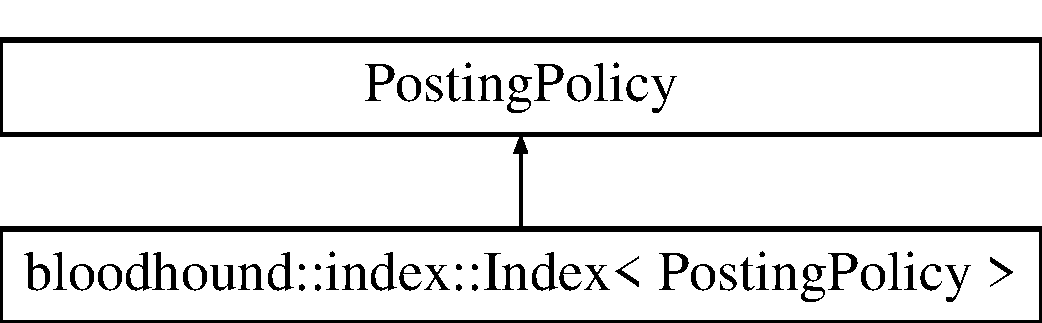
\includegraphics[height=2.000000cm]{classbloodhound_1_1index_1_1Index}
\end{center}
\end{figure}
\subsection*{Public Member Functions}
\begin{DoxyCompactItemize}
\item 
std\+::size\+\_\+t \hyperlink{classbloodhound_1_1index_1_1Index_aead1eb965d1607d25398b874cbd8a269}{get\+\_\+collection\+\_\+size} () const
\item 
\hyperlink{classbloodhound_1_1PostingList}{Posting\+List} \hyperlink{classbloodhound_1_1index_1_1Index_a24cadb41178b2cc81cf8f3e32a5dd516}{posting\+\_\+list} (\hyperlink{structbloodhound_1_1TermId}{Term\+Id} termid, bool load\+\_\+max\+\_\+scores=true)
\item 
\hyperlink{classbloodhound_1_1PostingList}{Posting\+List} \hyperlink{classbloodhound_1_1index_1_1Index_ac26271e4e2678e77d46017a24ed7eac5}{posting\+\_\+list} (\hyperlink{structbloodhound_1_1TermId}{Term\+Id} termid, double et\+\_\+threshold)
\item 
std\+::vector$<$ \hyperlink{classbloodhound_1_1PostingList}{Posting\+List} $>$ \hyperlink{classbloodhound_1_1index_1_1Index_ae36f606ee2206c44d44d0a11ae91b04c}{terms\+\_\+to\+\_\+postings} (const std\+::vector$<$ \hyperlink{structbloodhound_1_1TermId}{Term\+Id} $>$ terms)
\begin{DoxyCompactList}\small\item\em Converts a vector of terms to a vector of posting lists. \end{DoxyCompactList}\item 
void \hyperlink{classbloodhound_1_1index_1_1Index_a00eb8ae8cf8f24430fe170095c4aa4d9}{calc\+\_\+maxscores} ()
\end{DoxyCompactItemize}
\subsection*{Static Public Member Functions}
\begin{DoxyCompactItemize}
\item 
static \hyperlink{namespacebloodhound_a94032a3533df0a1b6d3435bad57e6499}{Lexicon} \hyperlink{classbloodhound_1_1index_1_1Index_a80968041cad02a4006fd4b633c279030}{load\+\_\+lexicon} (fs\+::path index\+\_\+dir)
\item 
static \hyperlink{namespacebloodhound_a687d80c6f992eba8b820bf30a482f4b4}{Max\+Scores} \hyperlink{classbloodhound_1_1index_1_1Index_a6333778f622dbf964ba6aea29a56dca0}{load\+\_\+maxscores} (fs\+::path index\+\_\+dir)
\item 
static std\+::tuple$<$ \hyperlink{namespacebloodhound_a94032a3533df0a1b6d3435bad57e6499}{Lexicon}, \hyperlink{namespacebloodhound_a687d80c6f992eba8b820bf30a482f4b4}{Max\+Scores} $>$ \hyperlink{classbloodhound_1_1index_1_1Index_a779359e7ce40294dd3d3666c00762700}{load\+\_\+mappings} (fs\+::path index\+\_\+dir)
\item 
static json\+::json \hyperlink{classbloodhound_1_1index_1_1Index_af0d9b72f7cf6b54d7bddbccd3c1898ce}{load\+\_\+meta} (fs\+::path meta\+\_\+file)
\item 
static void \hyperlink{classbloodhound_1_1index_1_1Index_a6f1e18905c2b5babd30f33467c79018a}{verify} (\hyperlink{classbloodhound_1_1index_1_1Index}{Index} \&index)
\item 
static void \hyperlink{classbloodhound_1_1index_1_1Index_a02e947bdd77e51dcb09db5b7f03f14c7}{write\+\_\+maxscores} (\hyperlink{classbloodhound_1_1index_1_1Index}{Index} \&index, fs\+::path out)
\item 
static \hyperlink{classbloodhound_1_1index_1_1Index}{Index} \hyperlink{classbloodhound_1_1index_1_1Index_a46fcfc3c54ecf18d4ff58a240557b567}{write\+\_\+maxscores} (fs\+::path index\+\_\+dir)
\item 
static \hyperlink{classbloodhound_1_1index_1_1Index}{Index} \hyperlink{classbloodhound_1_1index_1_1Index_ad4cd13bef623fc6b786f8003c8826b9c}{load\+\_\+index} (fs\+::path index\+\_\+dir, bool verify\+\_\+maxscores=false)
\end{DoxyCompactItemize}
\subsection*{Public Attributes}
\begin{DoxyCompactItemize}
\item 
\hyperlink{namespacebloodhound_a94032a3533df0a1b6d3435bad57e6499}{Lexicon} \hyperlink{classbloodhound_1_1index_1_1Index_a746d80c2fb411f512726c8d37cad78fc}{lexicon}
\end{DoxyCompactItemize}
\subsection*{Friends}
\begin{DoxyCompactItemize}
\item 
\hyperlink{classbloodhound_1_1index_1_1Index}{Index}$<$ \hyperlink{classbloodhound_1_1index_1_1InMemoryPostingPolicy}{In\+Memory\+Posting\+Policy} $>$ \hyperlink{classbloodhound_1_1index_1_1Index_a0343a97c005a2df437a955c308d376e6}{build\+\_\+index\+\_\+from\+\_\+ids} (const std\+::vector$<$ std\+::vector$<$ \hyperlink{structbloodhound_1_1TermWeight}{Term\+Weight} $>$$>$ \&input)
\item 
\hyperlink{classbloodhound_1_1index_1_1Index}{Index}$<$ \hyperlink{classbloodhound_1_1index_1_1InMemoryPostingPolicy}{In\+Memory\+Posting\+Policy} $>$ \hyperlink{classbloodhound_1_1index_1_1Index_aad81f0929f0b03479f3361a23d96573b}{sorted\+\_\+index} (const \hyperlink{classbloodhound_1_1index_1_1Index}{Index}$<$ \hyperlink{classbloodhound_1_1index_1_1InMemoryPostingPolicy}{In\+Memory\+Posting\+Policy} $>$ \&index)
\end{DoxyCompactItemize}


\subsection{Member Function Documentation}
\mbox{\Hypertarget{classbloodhound_1_1index_1_1Index_a00eb8ae8cf8f24430fe170095c4aa4d9}\label{classbloodhound_1_1index_1_1Index_a00eb8ae8cf8f24430fe170095c4aa4d9}} 
\index{bloodhound\+::index\+::\+Index@{bloodhound\+::index\+::\+Index}!calc\+\_\+maxscores@{calc\+\_\+maxscores}}
\index{calc\+\_\+maxscores@{calc\+\_\+maxscores}!bloodhound\+::index\+::\+Index@{bloodhound\+::index\+::\+Index}}
\subsubsection{\texorpdfstring{calc\+\_\+maxscores()}{calc\_maxscores()}}
{\footnotesize\ttfamily template$<$class Posting\+Policy = In\+Memory\+Posting\+Policy$>$ \\
void \hyperlink{classbloodhound_1_1index_1_1Index}{bloodhound\+::index\+::\+Index}$<$ Posting\+Policy $>$\+::calc\+\_\+maxscores (\begin{DoxyParamCaption}{ }\end{DoxyParamCaption})\hspace{0.3cm}{\ttfamily [inline]}}

\mbox{\Hypertarget{classbloodhound_1_1index_1_1Index_aead1eb965d1607d25398b874cbd8a269}\label{classbloodhound_1_1index_1_1Index_aead1eb965d1607d25398b874cbd8a269}} 
\index{bloodhound\+::index\+::\+Index@{bloodhound\+::index\+::\+Index}!get\+\_\+collection\+\_\+size@{get\+\_\+collection\+\_\+size}}
\index{get\+\_\+collection\+\_\+size@{get\+\_\+collection\+\_\+size}!bloodhound\+::index\+::\+Index@{bloodhound\+::index\+::\+Index}}
\subsubsection{\texorpdfstring{get\+\_\+collection\+\_\+size()}{get\_collection\_size()}}
{\footnotesize\ttfamily template$<$class Posting\+Policy = In\+Memory\+Posting\+Policy$>$ \\
std\+::size\+\_\+t \hyperlink{classbloodhound_1_1index_1_1Index}{bloodhound\+::index\+::\+Index}$<$ Posting\+Policy $>$\+::get\+\_\+collection\+\_\+size (\begin{DoxyParamCaption}{ }\end{DoxyParamCaption}) const\hspace{0.3cm}{\ttfamily [inline]}}

\mbox{\Hypertarget{classbloodhound_1_1index_1_1Index_ad4cd13bef623fc6b786f8003c8826b9c}\label{classbloodhound_1_1index_1_1Index_ad4cd13bef623fc6b786f8003c8826b9c}} 
\index{bloodhound\+::index\+::\+Index@{bloodhound\+::index\+::\+Index}!load\+\_\+index@{load\+\_\+index}}
\index{load\+\_\+index@{load\+\_\+index}!bloodhound\+::index\+::\+Index@{bloodhound\+::index\+::\+Index}}
\subsubsection{\texorpdfstring{load\+\_\+index()}{load\_index()}}
{\footnotesize\ttfamily template$<$class Posting\+Policy = In\+Memory\+Posting\+Policy$>$ \\
static \hyperlink{classbloodhound_1_1index_1_1Index}{Index} \hyperlink{classbloodhound_1_1index_1_1Index}{bloodhound\+::index\+::\+Index}$<$ Posting\+Policy $>$\+::load\+\_\+index (\begin{DoxyParamCaption}\item[{fs\+::path}]{index\+\_\+dir,  }\item[{bool}]{verify\+\_\+maxscores = {\ttfamily false} }\end{DoxyParamCaption})\hspace{0.3cm}{\ttfamily [inline]}, {\ttfamily [static]}}

\mbox{\Hypertarget{classbloodhound_1_1index_1_1Index_a80968041cad02a4006fd4b633c279030}\label{classbloodhound_1_1index_1_1Index_a80968041cad02a4006fd4b633c279030}} 
\index{bloodhound\+::index\+::\+Index@{bloodhound\+::index\+::\+Index}!load\+\_\+lexicon@{load\+\_\+lexicon}}
\index{load\+\_\+lexicon@{load\+\_\+lexicon}!bloodhound\+::index\+::\+Index@{bloodhound\+::index\+::\+Index}}
\subsubsection{\texorpdfstring{load\+\_\+lexicon()}{load\_lexicon()}}
{\footnotesize\ttfamily template$<$class Posting\+Policy = In\+Memory\+Posting\+Policy$>$ \\
static \hyperlink{namespacebloodhound_a94032a3533df0a1b6d3435bad57e6499}{Lexicon} \hyperlink{classbloodhound_1_1index_1_1Index}{bloodhound\+::index\+::\+Index}$<$ Posting\+Policy $>$\+::load\+\_\+lexicon (\begin{DoxyParamCaption}\item[{fs\+::path}]{index\+\_\+dir }\end{DoxyParamCaption})\hspace{0.3cm}{\ttfamily [inline]}, {\ttfamily [static]}}

\mbox{\Hypertarget{classbloodhound_1_1index_1_1Index_a779359e7ce40294dd3d3666c00762700}\label{classbloodhound_1_1index_1_1Index_a779359e7ce40294dd3d3666c00762700}} 
\index{bloodhound\+::index\+::\+Index@{bloodhound\+::index\+::\+Index}!load\+\_\+mappings@{load\+\_\+mappings}}
\index{load\+\_\+mappings@{load\+\_\+mappings}!bloodhound\+::index\+::\+Index@{bloodhound\+::index\+::\+Index}}
\subsubsection{\texorpdfstring{load\+\_\+mappings()}{load\_mappings()}}
{\footnotesize\ttfamily template$<$class Posting\+Policy = In\+Memory\+Posting\+Policy$>$ \\
static std\+::tuple$<$\hyperlink{namespacebloodhound_a94032a3533df0a1b6d3435bad57e6499}{Lexicon}, \hyperlink{namespacebloodhound_a687d80c6f992eba8b820bf30a482f4b4}{Max\+Scores}$>$ \hyperlink{classbloodhound_1_1index_1_1Index}{bloodhound\+::index\+::\+Index}$<$ Posting\+Policy $>$\+::load\+\_\+mappings (\begin{DoxyParamCaption}\item[{fs\+::path}]{index\+\_\+dir }\end{DoxyParamCaption})\hspace{0.3cm}{\ttfamily [inline]}, {\ttfamily [static]}}

\mbox{\Hypertarget{classbloodhound_1_1index_1_1Index_a6333778f622dbf964ba6aea29a56dca0}\label{classbloodhound_1_1index_1_1Index_a6333778f622dbf964ba6aea29a56dca0}} 
\index{bloodhound\+::index\+::\+Index@{bloodhound\+::index\+::\+Index}!load\+\_\+maxscores@{load\+\_\+maxscores}}
\index{load\+\_\+maxscores@{load\+\_\+maxscores}!bloodhound\+::index\+::\+Index@{bloodhound\+::index\+::\+Index}}
\subsubsection{\texorpdfstring{load\+\_\+maxscores()}{load\_maxscores()}}
{\footnotesize\ttfamily template$<$class Posting\+Policy = In\+Memory\+Posting\+Policy$>$ \\
static \hyperlink{namespacebloodhound_a687d80c6f992eba8b820bf30a482f4b4}{Max\+Scores} \hyperlink{classbloodhound_1_1index_1_1Index}{bloodhound\+::index\+::\+Index}$<$ Posting\+Policy $>$\+::load\+\_\+maxscores (\begin{DoxyParamCaption}\item[{fs\+::path}]{index\+\_\+dir }\end{DoxyParamCaption})\hspace{0.3cm}{\ttfamily [inline]}, {\ttfamily [static]}}

\mbox{\Hypertarget{classbloodhound_1_1index_1_1Index_af0d9b72f7cf6b54d7bddbccd3c1898ce}\label{classbloodhound_1_1index_1_1Index_af0d9b72f7cf6b54d7bddbccd3c1898ce}} 
\index{bloodhound\+::index\+::\+Index@{bloodhound\+::index\+::\+Index}!load\+\_\+meta@{load\+\_\+meta}}
\index{load\+\_\+meta@{load\+\_\+meta}!bloodhound\+::index\+::\+Index@{bloodhound\+::index\+::\+Index}}
\subsubsection{\texorpdfstring{load\+\_\+meta()}{load\_meta()}}
{\footnotesize\ttfamily template$<$class Posting\+Policy = In\+Memory\+Posting\+Policy$>$ \\
static json\+::json \hyperlink{classbloodhound_1_1index_1_1Index}{bloodhound\+::index\+::\+Index}$<$ Posting\+Policy $>$\+::load\+\_\+meta (\begin{DoxyParamCaption}\item[{fs\+::path}]{meta\+\_\+file }\end{DoxyParamCaption})\hspace{0.3cm}{\ttfamily [inline]}, {\ttfamily [static]}}

\mbox{\Hypertarget{classbloodhound_1_1index_1_1Index_a24cadb41178b2cc81cf8f3e32a5dd516}\label{classbloodhound_1_1index_1_1Index_a24cadb41178b2cc81cf8f3e32a5dd516}} 
\index{bloodhound\+::index\+::\+Index@{bloodhound\+::index\+::\+Index}!posting\+\_\+list@{posting\+\_\+list}}
\index{posting\+\_\+list@{posting\+\_\+list}!bloodhound\+::index\+::\+Index@{bloodhound\+::index\+::\+Index}}
\subsubsection{\texorpdfstring{posting\+\_\+list()}{posting\_list()}\hspace{0.1cm}{\footnotesize\ttfamily [1/2]}}
{\footnotesize\ttfamily template$<$class Posting\+Policy = In\+Memory\+Posting\+Policy$>$ \\
\hyperlink{classbloodhound_1_1PostingList}{Posting\+List} \hyperlink{classbloodhound_1_1index_1_1Index}{bloodhound\+::index\+::\+Index}$<$ Posting\+Policy $>$\+::posting\+\_\+list (\begin{DoxyParamCaption}\item[{\hyperlink{structbloodhound_1_1TermId}{Term\+Id}}]{termid,  }\item[{bool}]{load\+\_\+max\+\_\+scores = {\ttfamily true} }\end{DoxyParamCaption})\hspace{0.3cm}{\ttfamily [inline]}}

\mbox{\Hypertarget{classbloodhound_1_1index_1_1Index_ac26271e4e2678e77d46017a24ed7eac5}\label{classbloodhound_1_1index_1_1Index_ac26271e4e2678e77d46017a24ed7eac5}} 
\index{bloodhound\+::index\+::\+Index@{bloodhound\+::index\+::\+Index}!posting\+\_\+list@{posting\+\_\+list}}
\index{posting\+\_\+list@{posting\+\_\+list}!bloodhound\+::index\+::\+Index@{bloodhound\+::index\+::\+Index}}
\subsubsection{\texorpdfstring{posting\+\_\+list()}{posting\_list()}\hspace{0.1cm}{\footnotesize\ttfamily [2/2]}}
{\footnotesize\ttfamily template$<$class Posting\+Policy = In\+Memory\+Posting\+Policy$>$ \\
\hyperlink{classbloodhound_1_1PostingList}{Posting\+List} \hyperlink{classbloodhound_1_1index_1_1Index}{bloodhound\+::index\+::\+Index}$<$ Posting\+Policy $>$\+::posting\+\_\+list (\begin{DoxyParamCaption}\item[{\hyperlink{structbloodhound_1_1TermId}{Term\+Id}}]{termid,  }\item[{double}]{et\+\_\+threshold }\end{DoxyParamCaption})\hspace{0.3cm}{\ttfamily [inline]}}

\mbox{\Hypertarget{classbloodhound_1_1index_1_1Index_ae36f606ee2206c44d44d0a11ae91b04c}\label{classbloodhound_1_1index_1_1Index_ae36f606ee2206c44d44d0a11ae91b04c}} 
\index{bloodhound\+::index\+::\+Index@{bloodhound\+::index\+::\+Index}!terms\+\_\+to\+\_\+postings@{terms\+\_\+to\+\_\+postings}}
\index{terms\+\_\+to\+\_\+postings@{terms\+\_\+to\+\_\+postings}!bloodhound\+::index\+::\+Index@{bloodhound\+::index\+::\+Index}}
\subsubsection{\texorpdfstring{terms\+\_\+to\+\_\+postings()}{terms\_to\_postings()}}
{\footnotesize\ttfamily template$<$class Posting\+Policy = In\+Memory\+Posting\+Policy$>$ \\
std\+::vector$<$\hyperlink{classbloodhound_1_1PostingList}{Posting\+List}$>$ \hyperlink{classbloodhound_1_1index_1_1Index}{bloodhound\+::index\+::\+Index}$<$ Posting\+Policy $>$\+::terms\+\_\+to\+\_\+postings (\begin{DoxyParamCaption}\item[{const std\+::vector$<$ \hyperlink{structbloodhound_1_1TermId}{Term\+Id} $>$}]{terms }\end{DoxyParamCaption})\hspace{0.3cm}{\ttfamily [inline]}}



Converts a vector of terms to a vector of posting lists. 

\mbox{\Hypertarget{classbloodhound_1_1index_1_1Index_a6f1e18905c2b5babd30f33467c79018a}\label{classbloodhound_1_1index_1_1Index_a6f1e18905c2b5babd30f33467c79018a}} 
\index{bloodhound\+::index\+::\+Index@{bloodhound\+::index\+::\+Index}!verify@{verify}}
\index{verify@{verify}!bloodhound\+::index\+::\+Index@{bloodhound\+::index\+::\+Index}}
\subsubsection{\texorpdfstring{verify()}{verify()}}
{\footnotesize\ttfamily template$<$class Posting\+Policy = In\+Memory\+Posting\+Policy$>$ \\
static void \hyperlink{classbloodhound_1_1index_1_1Index}{bloodhound\+::index\+::\+Index}$<$ Posting\+Policy $>$\+::verify (\begin{DoxyParamCaption}\item[{\hyperlink{classbloodhound_1_1index_1_1Index}{Index}$<$ Posting\+Policy $>$ \&}]{index }\end{DoxyParamCaption})\hspace{0.3cm}{\ttfamily [inline]}, {\ttfamily [static]}}

\mbox{\Hypertarget{classbloodhound_1_1index_1_1Index_a02e947bdd77e51dcb09db5b7f03f14c7}\label{classbloodhound_1_1index_1_1Index_a02e947bdd77e51dcb09db5b7f03f14c7}} 
\index{bloodhound\+::index\+::\+Index@{bloodhound\+::index\+::\+Index}!write\+\_\+maxscores@{write\+\_\+maxscores}}
\index{write\+\_\+maxscores@{write\+\_\+maxscores}!bloodhound\+::index\+::\+Index@{bloodhound\+::index\+::\+Index}}
\subsubsection{\texorpdfstring{write\+\_\+maxscores()}{write\_maxscores()}\hspace{0.1cm}{\footnotesize\ttfamily [1/2]}}
{\footnotesize\ttfamily template$<$class Posting\+Policy = In\+Memory\+Posting\+Policy$>$ \\
static void \hyperlink{classbloodhound_1_1index_1_1Index}{bloodhound\+::index\+::\+Index}$<$ Posting\+Policy $>$\+::write\+\_\+maxscores (\begin{DoxyParamCaption}\item[{\hyperlink{classbloodhound_1_1index_1_1Index}{Index}$<$ Posting\+Policy $>$ \&}]{index,  }\item[{fs\+::path}]{out }\end{DoxyParamCaption})\hspace{0.3cm}{\ttfamily [inline]}, {\ttfamily [static]}}

\mbox{\Hypertarget{classbloodhound_1_1index_1_1Index_a46fcfc3c54ecf18d4ff58a240557b567}\label{classbloodhound_1_1index_1_1Index_a46fcfc3c54ecf18d4ff58a240557b567}} 
\index{bloodhound\+::index\+::\+Index@{bloodhound\+::index\+::\+Index}!write\+\_\+maxscores@{write\+\_\+maxscores}}
\index{write\+\_\+maxscores@{write\+\_\+maxscores}!bloodhound\+::index\+::\+Index@{bloodhound\+::index\+::\+Index}}
\subsubsection{\texorpdfstring{write\+\_\+maxscores()}{write\_maxscores()}\hspace{0.1cm}{\footnotesize\ttfamily [2/2]}}
{\footnotesize\ttfamily template$<$class Posting\+Policy = In\+Memory\+Posting\+Policy$>$ \\
static \hyperlink{classbloodhound_1_1index_1_1Index}{Index} \hyperlink{classbloodhound_1_1index_1_1Index}{bloodhound\+::index\+::\+Index}$<$ Posting\+Policy $>$\+::write\+\_\+maxscores (\begin{DoxyParamCaption}\item[{fs\+::path}]{index\+\_\+dir }\end{DoxyParamCaption})\hspace{0.3cm}{\ttfamily [inline]}, {\ttfamily [static]}}



\subsection{Friends And Related Function Documentation}
\mbox{\Hypertarget{classbloodhound_1_1index_1_1Index_a0343a97c005a2df437a955c308d376e6}\label{classbloodhound_1_1index_1_1Index_a0343a97c005a2df437a955c308d376e6}} 
\index{bloodhound\+::index\+::\+Index@{bloodhound\+::index\+::\+Index}!build\+\_\+index\+\_\+from\+\_\+ids@{build\+\_\+index\+\_\+from\+\_\+ids}}
\index{build\+\_\+index\+\_\+from\+\_\+ids@{build\+\_\+index\+\_\+from\+\_\+ids}!bloodhound\+::index\+::\+Index@{bloodhound\+::index\+::\+Index}}
\subsubsection{\texorpdfstring{build\+\_\+index\+\_\+from\+\_\+ids}{build\_index\_from\_ids}}
{\footnotesize\ttfamily template$<$class Posting\+Policy = In\+Memory\+Posting\+Policy$>$ \\
\hyperlink{classbloodhound_1_1index_1_1Index}{Index}$<$\hyperlink{classbloodhound_1_1index_1_1InMemoryPostingPolicy}{In\+Memory\+Posting\+Policy}$>$ build\+\_\+index\+\_\+from\+\_\+ids (\begin{DoxyParamCaption}\item[{const std\+::vector$<$ std\+::vector$<$ \hyperlink{structbloodhound_1_1TermWeight}{Term\+Weight} $>$$>$ \&}]{input }\end{DoxyParamCaption})\hspace{0.3cm}{\ttfamily [friend]}}

Builds an index based on a collection represented by term I\+Ds.

This function is not efficient and only meant for testing other functionalities. \mbox{\Hypertarget{classbloodhound_1_1index_1_1Index_aad81f0929f0b03479f3361a23d96573b}\label{classbloodhound_1_1index_1_1Index_aad81f0929f0b03479f3361a23d96573b}} 
\index{bloodhound\+::index\+::\+Index@{bloodhound\+::index\+::\+Index}!sorted\+\_\+index@{sorted\+\_\+index}}
\index{sorted\+\_\+index@{sorted\+\_\+index}!bloodhound\+::index\+::\+Index@{bloodhound\+::index\+::\+Index}}
\subsubsection{\texorpdfstring{sorted\+\_\+index}{sorted\_index}}
{\footnotesize\ttfamily template$<$class Posting\+Policy = In\+Memory\+Posting\+Policy$>$ \\
\hyperlink{classbloodhound_1_1index_1_1Index}{Index}$<$\hyperlink{classbloodhound_1_1index_1_1InMemoryPostingPolicy}{In\+Memory\+Posting\+Policy}$>$ sorted\+\_\+index (\begin{DoxyParamCaption}\item[{const \hyperlink{classbloodhound_1_1index_1_1Index}{Index}$<$ \hyperlink{classbloodhound_1_1index_1_1InMemoryPostingPolicy}{In\+Memory\+Posting\+Policy} $>$ \&}]{index }\end{DoxyParamCaption})\hspace{0.3cm}{\ttfamily [friend]}}



\subsection{Member Data Documentation}
\mbox{\Hypertarget{classbloodhound_1_1index_1_1Index_a746d80c2fb411f512726c8d37cad78fc}\label{classbloodhound_1_1index_1_1Index_a746d80c2fb411f512726c8d37cad78fc}} 
\index{bloodhound\+::index\+::\+Index@{bloodhound\+::index\+::\+Index}!lexicon@{lexicon}}
\index{lexicon@{lexicon}!bloodhound\+::index\+::\+Index@{bloodhound\+::index\+::\+Index}}
\subsubsection{\texorpdfstring{lexicon}{lexicon}}
{\footnotesize\ttfamily template$<$class Posting\+Policy = In\+Memory\+Posting\+Policy$>$ \\
\hyperlink{namespacebloodhound_a94032a3533df0a1b6d3435bad57e6499}{Lexicon} \hyperlink{classbloodhound_1_1index_1_1Index}{bloodhound\+::index\+::\+Index}$<$ Posting\+Policy $>$\+::lexicon}



The documentation for this class was generated from the following file\+:\begin{DoxyCompactItemize}
\item 
include/\hyperlink{index_8hpp}{index.\+hpp}\end{DoxyCompactItemize}

\hypertarget{classirkit_1_1IndexBuilder}{}\section{irkit\+:\+:Index\+Builder$<$ Doc, Term, Term\+Id, Freq $>$ Class Template Reference}
\label{classirkit_1_1IndexBuilder}\index{irkit\+::\+Index\+Builder$<$ Doc, Term, Term\+Id, Freq $>$@{irkit\+::\+Index\+Builder$<$ Doc, Term, Term\+Id, Freq $>$}}


{\ttfamily \#include $<$index.\+hpp$>$}

\subsection*{Public Member Functions}
\begin{DoxyCompactItemize}
\item 
\hyperlink{classirkit_1_1IndexBuilder_ab56476b7728ed2618b8de7511dfe2427}{Index\+Builder} ()
\item 
void \hyperlink{classirkit_1_1IndexBuilder_a8a18c112d48e21a89aefa9a931a536ab}{add\+\_\+document} ()
\begin{DoxyCompactList}\small\item\em Initiates a new document with an incremented ID. \end{DoxyCompactList}\item 
void \hyperlink{classirkit_1_1IndexBuilder_a31b062283c9b7203ce4a65a5bd744fae}{add\+\_\+document} (Doc doc)
\begin{DoxyCompactList}\small\item\em Initiates a new document with the given ID. \end{DoxyCompactList}\item 
void \hyperlink{classirkit_1_1IndexBuilder_a6005b21c9a24cb54fe54957e21c0487a}{add\+\_\+term} (const Term \&term)
\begin{DoxyCompactList}\small\item\em Adds a term to the current document. \end{DoxyCompactList}\item 
Freq \hyperlink{classirkit_1_1IndexBuilder_ac4c8613d07637de4b67d61df2910bbd0}{document\+\_\+frequency} (Term\+Id term\+\_\+id)
\begin{DoxyCompactList}\small\item\em Returns the document frequency of the given term. \end{DoxyCompactList}\item 
std\+::size\+\_\+t \hyperlink{classirkit_1_1IndexBuilder_a81221fd5879c7d68d4d6bff6005b8cd7}{collection\+\_\+size} ()
\begin{DoxyCompactList}\small\item\em Returns the number of the accumulated documents. \end{DoxyCompactList}\item 
void \hyperlink{classirkit_1_1IndexBuilder_a242138da460b9853fc6aebb5b8c59c86}{sort\+\_\+terms} ()
\begin{DoxyCompactList}\small\item\em Sorts the terms, and all related structures, lexicographically. \end{DoxyCompactList}\item 
void \hyperlink{classirkit_1_1IndexBuilder_a7c81e735e585ec41a7e5e334e4416874}{write\+\_\+terms} (std\+::ostream \&out)
\begin{DoxyCompactList}\small\item\em Writes new-\/line-\/delimited sorted list of terms. \end{DoxyCompactList}\item 
void \hyperlink{classirkit_1_1IndexBuilder_af8d8c6c446a064ec7c9b2a05b522555e}{write\+\_\+document\+\_\+ids} (std\+::ostream \&out, std\+::ostream \&off)
\begin{DoxyCompactList}\small\item\em Writes document I\+Ds. \end{DoxyCompactList}\item 
void \hyperlink{classirkit_1_1IndexBuilder_aba0b947f29e491205adf3df3f862e58e}{write\+\_\+document\+\_\+counts} (std\+::ostream \&out, std\+::ostream \&off)
\begin{DoxyCompactList}\small\item\em Writes term-\/document frequencies (tf). \end{DoxyCompactList}\item 
void \hyperlink{classirkit_1_1IndexBuilder_a57c15d23588f70b78b49a6392ef61be8}{write\+\_\+document\+\_\+frequencies} (std\+::ostream \&out)
\begin{DoxyCompactList}\small\item\em Writes document frequencies (df). \end{DoxyCompactList}\end{DoxyCompactItemize}
\subsection*{Protected Attributes}
\begin{DoxyCompactItemize}
\item 
Doc \hyperlink{classirkit_1_1IndexBuilder_a52d46fb2bd04b9e5ee0e9fdcf98e2f7b}{current\+\_\+doc\+\_\+}
\item 
std\+::optional$<$ std\+::vector$<$ Term $>$ $>$ \hyperlink{classirkit_1_1IndexBuilder_a7a6b13e964f05c659fe17cf61a9738e9}{sorted\+\_\+terms\+\_\+}
\item 
std\+::vector$<$ std\+::vector$<$ Doc\+Freq $>$ $>$ \hyperlink{classirkit_1_1IndexBuilder_a4dcd133d2afe183e6f5bb379592391c4}{postings\+\_\+}
\item 
std\+::vector$<$ std\+::size\+\_\+t $>$ \hyperlink{classirkit_1_1IndexBuilder_aaa27520f3a0fb37dba049d2c26ad9484}{term\+\_\+occurrences\+\_\+}
\item 
std\+::unordered\+\_\+map$<$ Term, Term\+Id $>$ \hyperlink{classirkit_1_1IndexBuilder_aeebb03b89eeab532f62239e4ea4f0bee}{term\+\_\+map\+\_\+}
\end{DoxyCompactItemize}


\subsection{Constructor \& Destructor Documentation}
\mbox{\Hypertarget{classirkit_1_1IndexBuilder_ab56476b7728ed2618b8de7511dfe2427}\label{classirkit_1_1IndexBuilder_ab56476b7728ed2618b8de7511dfe2427}} 
\index{irkit\+::\+Index\+Builder@{irkit\+::\+Index\+Builder}!Index\+Builder@{Index\+Builder}}
\index{Index\+Builder@{Index\+Builder}!irkit\+::\+Index\+Builder@{irkit\+::\+Index\+Builder}}
\subsubsection{\texorpdfstring{Index\+Builder()}{IndexBuilder()}}
{\footnotesize\ttfamily template$<$class Doc  = std\+::size\+\_\+t, class Term  = std\+::string, class Term\+Id  = std\+::size\+\_\+t, class Freq  = std\+::size\+\_\+t$>$ \\
\hyperlink{classirkit_1_1IndexBuilder}{irkit\+::\+Index\+Builder}$<$ Doc, Term, Term\+Id, Freq $>$\+::\hyperlink{classirkit_1_1IndexBuilder}{Index\+Builder} (\begin{DoxyParamCaption}{ }\end{DoxyParamCaption})\hspace{0.3cm}{\ttfamily [inline]}}



\subsection{Member Function Documentation}
\mbox{\Hypertarget{classirkit_1_1IndexBuilder_a8a18c112d48e21a89aefa9a931a536ab}\label{classirkit_1_1IndexBuilder_a8a18c112d48e21a89aefa9a931a536ab}} 
\index{irkit\+::\+Index\+Builder@{irkit\+::\+Index\+Builder}!add\+\_\+document@{add\+\_\+document}}
\index{add\+\_\+document@{add\+\_\+document}!irkit\+::\+Index\+Builder@{irkit\+::\+Index\+Builder}}
\subsubsection{\texorpdfstring{add\+\_\+document()}{add\_document()}\hspace{0.1cm}{\footnotesize\ttfamily [1/2]}}
{\footnotesize\ttfamily template$<$class Doc  = std\+::size\+\_\+t, class Term  = std\+::string, class Term\+Id  = std\+::size\+\_\+t, class Freq  = std\+::size\+\_\+t$>$ \\
void \hyperlink{classirkit_1_1IndexBuilder}{irkit\+::\+Index\+Builder}$<$ Doc, Term, Term\+Id, Freq $>$\+::add\+\_\+document (\begin{DoxyParamCaption}{ }\end{DoxyParamCaption})\hspace{0.3cm}{\ttfamily [inline]}}



Initiates a new document with an incremented ID. 

\mbox{\Hypertarget{classirkit_1_1IndexBuilder_a31b062283c9b7203ce4a65a5bd744fae}\label{classirkit_1_1IndexBuilder_a31b062283c9b7203ce4a65a5bd744fae}} 
\index{irkit\+::\+Index\+Builder@{irkit\+::\+Index\+Builder}!add\+\_\+document@{add\+\_\+document}}
\index{add\+\_\+document@{add\+\_\+document}!irkit\+::\+Index\+Builder@{irkit\+::\+Index\+Builder}}
\subsubsection{\texorpdfstring{add\+\_\+document()}{add\_document()}\hspace{0.1cm}{\footnotesize\ttfamily [2/2]}}
{\footnotesize\ttfamily template$<$class Doc  = std\+::size\+\_\+t, class Term  = std\+::string, class Term\+Id  = std\+::size\+\_\+t, class Freq  = std\+::size\+\_\+t$>$ \\
void \hyperlink{classirkit_1_1IndexBuilder}{irkit\+::\+Index\+Builder}$<$ Doc, Term, Term\+Id, Freq $>$\+::add\+\_\+document (\begin{DoxyParamCaption}\item[{Doc}]{doc }\end{DoxyParamCaption})\hspace{0.3cm}{\ttfamily [inline]}}



Initiates a new document with the given ID. 

\mbox{\Hypertarget{classirkit_1_1IndexBuilder_a6005b21c9a24cb54fe54957e21c0487a}\label{classirkit_1_1IndexBuilder_a6005b21c9a24cb54fe54957e21c0487a}} 
\index{irkit\+::\+Index\+Builder@{irkit\+::\+Index\+Builder}!add\+\_\+term@{add\+\_\+term}}
\index{add\+\_\+term@{add\+\_\+term}!irkit\+::\+Index\+Builder@{irkit\+::\+Index\+Builder}}
\subsubsection{\texorpdfstring{add\+\_\+term()}{add\_term()}}
{\footnotesize\ttfamily template$<$class Doc  = std\+::size\+\_\+t, class Term  = std\+::string, class Term\+Id  = std\+::size\+\_\+t, class Freq  = std\+::size\+\_\+t$>$ \\
void \hyperlink{classirkit_1_1IndexBuilder}{irkit\+::\+Index\+Builder}$<$ Doc, Term, Term\+Id, Freq $>$\+::add\+\_\+term (\begin{DoxyParamCaption}\item[{const Term \&}]{term }\end{DoxyParamCaption})\hspace{0.3cm}{\ttfamily [inline]}}



Adds a term to the current document. 

\mbox{\Hypertarget{classirkit_1_1IndexBuilder_a81221fd5879c7d68d4d6bff6005b8cd7}\label{classirkit_1_1IndexBuilder_a81221fd5879c7d68d4d6bff6005b8cd7}} 
\index{irkit\+::\+Index\+Builder@{irkit\+::\+Index\+Builder}!collection\+\_\+size@{collection\+\_\+size}}
\index{collection\+\_\+size@{collection\+\_\+size}!irkit\+::\+Index\+Builder@{irkit\+::\+Index\+Builder}}
\subsubsection{\texorpdfstring{collection\+\_\+size()}{collection\_size()}}
{\footnotesize\ttfamily template$<$class Doc  = std\+::size\+\_\+t, class Term  = std\+::string, class Term\+Id  = std\+::size\+\_\+t, class Freq  = std\+::size\+\_\+t$>$ \\
std\+::size\+\_\+t \hyperlink{classirkit_1_1IndexBuilder}{irkit\+::\+Index\+Builder}$<$ Doc, Term, Term\+Id, Freq $>$\+::collection\+\_\+size (\begin{DoxyParamCaption}{ }\end{DoxyParamCaption})\hspace{0.3cm}{\ttfamily [inline]}}



Returns the number of the accumulated documents. 

\mbox{\Hypertarget{classirkit_1_1IndexBuilder_ac4c8613d07637de4b67d61df2910bbd0}\label{classirkit_1_1IndexBuilder_ac4c8613d07637de4b67d61df2910bbd0}} 
\index{irkit\+::\+Index\+Builder@{irkit\+::\+Index\+Builder}!document\+\_\+frequency@{document\+\_\+frequency}}
\index{document\+\_\+frequency@{document\+\_\+frequency}!irkit\+::\+Index\+Builder@{irkit\+::\+Index\+Builder}}
\subsubsection{\texorpdfstring{document\+\_\+frequency()}{document\_frequency()}}
{\footnotesize\ttfamily template$<$class Doc  = std\+::size\+\_\+t, class Term  = std\+::string, class Term\+Id  = std\+::size\+\_\+t, class Freq  = std\+::size\+\_\+t$>$ \\
Freq \hyperlink{classirkit_1_1IndexBuilder}{irkit\+::\+Index\+Builder}$<$ Doc, Term, Term\+Id, Freq $>$\+::document\+\_\+frequency (\begin{DoxyParamCaption}\item[{Term\+Id}]{term\+\_\+id }\end{DoxyParamCaption})\hspace{0.3cm}{\ttfamily [inline]}}



Returns the document frequency of the given term. 

\mbox{\Hypertarget{classirkit_1_1IndexBuilder_a242138da460b9853fc6aebb5b8c59c86}\label{classirkit_1_1IndexBuilder_a242138da460b9853fc6aebb5b8c59c86}} 
\index{irkit\+::\+Index\+Builder@{irkit\+::\+Index\+Builder}!sort\+\_\+terms@{sort\+\_\+terms}}
\index{sort\+\_\+terms@{sort\+\_\+terms}!irkit\+::\+Index\+Builder@{irkit\+::\+Index\+Builder}}
\subsubsection{\texorpdfstring{sort\+\_\+terms()}{sort\_terms()}}
{\footnotesize\ttfamily template$<$class Doc  = std\+::size\+\_\+t, class Term  = std\+::string, class Term\+Id  = std\+::size\+\_\+t, class Freq  = std\+::size\+\_\+t$>$ \\
void \hyperlink{classirkit_1_1IndexBuilder}{irkit\+::\+Index\+Builder}$<$ Doc, Term, Term\+Id, Freq $>$\+::sort\+\_\+terms (\begin{DoxyParamCaption}{ }\end{DoxyParamCaption})\hspace{0.3cm}{\ttfamily [inline]}}



Sorts the terms, and all related structures, lexicographically. 

\mbox{\Hypertarget{classirkit_1_1IndexBuilder_aba0b947f29e491205adf3df3f862e58e}\label{classirkit_1_1IndexBuilder_aba0b947f29e491205adf3df3f862e58e}} 
\index{irkit\+::\+Index\+Builder@{irkit\+::\+Index\+Builder}!write\+\_\+document\+\_\+counts@{write\+\_\+document\+\_\+counts}}
\index{write\+\_\+document\+\_\+counts@{write\+\_\+document\+\_\+counts}!irkit\+::\+Index\+Builder@{irkit\+::\+Index\+Builder}}
\subsubsection{\texorpdfstring{write\+\_\+document\+\_\+counts()}{write\_document\_counts()}}
{\footnotesize\ttfamily template$<$class Doc  = std\+::size\+\_\+t, class Term  = std\+::string, class Term\+Id  = std\+::size\+\_\+t, class Freq  = std\+::size\+\_\+t$>$ \\
void \hyperlink{classirkit_1_1IndexBuilder}{irkit\+::\+Index\+Builder}$<$ Doc, Term, Term\+Id, Freq $>$\+::write\+\_\+document\+\_\+counts (\begin{DoxyParamCaption}\item[{std\+::ostream \&}]{out,  }\item[{std\+::ostream \&}]{off }\end{DoxyParamCaption})\hspace{0.3cm}{\ttfamily [inline]}}



Writes term-\/document frequencies (tf). 

\mbox{\Hypertarget{classirkit_1_1IndexBuilder_a57c15d23588f70b78b49a6392ef61be8}\label{classirkit_1_1IndexBuilder_a57c15d23588f70b78b49a6392ef61be8}} 
\index{irkit\+::\+Index\+Builder@{irkit\+::\+Index\+Builder}!write\+\_\+document\+\_\+frequencies@{write\+\_\+document\+\_\+frequencies}}
\index{write\+\_\+document\+\_\+frequencies@{write\+\_\+document\+\_\+frequencies}!irkit\+::\+Index\+Builder@{irkit\+::\+Index\+Builder}}
\subsubsection{\texorpdfstring{write\+\_\+document\+\_\+frequencies()}{write\_document\_frequencies()}}
{\footnotesize\ttfamily template$<$class Doc  = std\+::size\+\_\+t, class Term  = std\+::string, class Term\+Id  = std\+::size\+\_\+t, class Freq  = std\+::size\+\_\+t$>$ \\
void \hyperlink{classirkit_1_1IndexBuilder}{irkit\+::\+Index\+Builder}$<$ Doc, Term, Term\+Id, Freq $>$\+::write\+\_\+document\+\_\+frequencies (\begin{DoxyParamCaption}\item[{std\+::ostream \&}]{out }\end{DoxyParamCaption})\hspace{0.3cm}{\ttfamily [inline]}}



Writes document frequencies (df). 

\mbox{\Hypertarget{classirkit_1_1IndexBuilder_af8d8c6c446a064ec7c9b2a05b522555e}\label{classirkit_1_1IndexBuilder_af8d8c6c446a064ec7c9b2a05b522555e}} 
\index{irkit\+::\+Index\+Builder@{irkit\+::\+Index\+Builder}!write\+\_\+document\+\_\+ids@{write\+\_\+document\+\_\+ids}}
\index{write\+\_\+document\+\_\+ids@{write\+\_\+document\+\_\+ids}!irkit\+::\+Index\+Builder@{irkit\+::\+Index\+Builder}}
\subsubsection{\texorpdfstring{write\+\_\+document\+\_\+ids()}{write\_document\_ids()}}
{\footnotesize\ttfamily template$<$class Doc  = std\+::size\+\_\+t, class Term  = std\+::string, class Term\+Id  = std\+::size\+\_\+t, class Freq  = std\+::size\+\_\+t$>$ \\
void \hyperlink{classirkit_1_1IndexBuilder}{irkit\+::\+Index\+Builder}$<$ Doc, Term, Term\+Id, Freq $>$\+::write\+\_\+document\+\_\+ids (\begin{DoxyParamCaption}\item[{std\+::ostream \&}]{out,  }\item[{std\+::ostream \&}]{off }\end{DoxyParamCaption})\hspace{0.3cm}{\ttfamily [inline]}}



Writes document I\+Ds. 

\mbox{\Hypertarget{classirkit_1_1IndexBuilder_a7c81e735e585ec41a7e5e334e4416874}\label{classirkit_1_1IndexBuilder_a7c81e735e585ec41a7e5e334e4416874}} 
\index{irkit\+::\+Index\+Builder@{irkit\+::\+Index\+Builder}!write\+\_\+terms@{write\+\_\+terms}}
\index{write\+\_\+terms@{write\+\_\+terms}!irkit\+::\+Index\+Builder@{irkit\+::\+Index\+Builder}}
\subsubsection{\texorpdfstring{write\+\_\+terms()}{write\_terms()}}
{\footnotesize\ttfamily template$<$class Doc  = std\+::size\+\_\+t, class Term  = std\+::string, class Term\+Id  = std\+::size\+\_\+t, class Freq  = std\+::size\+\_\+t$>$ \\
void \hyperlink{classirkit_1_1IndexBuilder}{irkit\+::\+Index\+Builder}$<$ Doc, Term, Term\+Id, Freq $>$\+::write\+\_\+terms (\begin{DoxyParamCaption}\item[{std\+::ostream \&}]{out }\end{DoxyParamCaption})\hspace{0.3cm}{\ttfamily [inline]}}



Writes new-\/line-\/delimited sorted list of terms. 



\subsection{Member Data Documentation}
\mbox{\Hypertarget{classirkit_1_1IndexBuilder_a52d46fb2bd04b9e5ee0e9fdcf98e2f7b}\label{classirkit_1_1IndexBuilder_a52d46fb2bd04b9e5ee0e9fdcf98e2f7b}} 
\index{irkit\+::\+Index\+Builder@{irkit\+::\+Index\+Builder}!current\+\_\+doc\+\_\+@{current\+\_\+doc\+\_\+}}
\index{current\+\_\+doc\+\_\+@{current\+\_\+doc\+\_\+}!irkit\+::\+Index\+Builder@{irkit\+::\+Index\+Builder}}
\subsubsection{\texorpdfstring{current\+\_\+doc\+\_\+}{current\_doc\_}}
{\footnotesize\ttfamily template$<$class Doc  = std\+::size\+\_\+t, class Term  = std\+::string, class Term\+Id  = std\+::size\+\_\+t, class Freq  = std\+::size\+\_\+t$>$ \\
Doc \hyperlink{classirkit_1_1IndexBuilder}{irkit\+::\+Index\+Builder}$<$ Doc, Term, Term\+Id, Freq $>$\+::current\+\_\+doc\+\_\+\hspace{0.3cm}{\ttfamily [protected]}}

\mbox{\Hypertarget{classirkit_1_1IndexBuilder_a4dcd133d2afe183e6f5bb379592391c4}\label{classirkit_1_1IndexBuilder_a4dcd133d2afe183e6f5bb379592391c4}} 
\index{irkit\+::\+Index\+Builder@{irkit\+::\+Index\+Builder}!postings\+\_\+@{postings\+\_\+}}
\index{postings\+\_\+@{postings\+\_\+}!irkit\+::\+Index\+Builder@{irkit\+::\+Index\+Builder}}
\subsubsection{\texorpdfstring{postings\+\_\+}{postings\_}}
{\footnotesize\ttfamily template$<$class Doc  = std\+::size\+\_\+t, class Term  = std\+::string, class Term\+Id  = std\+::size\+\_\+t, class Freq  = std\+::size\+\_\+t$>$ \\
std\+::vector$<$std\+::vector$<$Doc\+Freq$>$ $>$ \hyperlink{classirkit_1_1IndexBuilder}{irkit\+::\+Index\+Builder}$<$ Doc, Term, Term\+Id, Freq $>$\+::postings\+\_\+\hspace{0.3cm}{\ttfamily [protected]}}

\mbox{\Hypertarget{classirkit_1_1IndexBuilder_a7a6b13e964f05c659fe17cf61a9738e9}\label{classirkit_1_1IndexBuilder_a7a6b13e964f05c659fe17cf61a9738e9}} 
\index{irkit\+::\+Index\+Builder@{irkit\+::\+Index\+Builder}!sorted\+\_\+terms\+\_\+@{sorted\+\_\+terms\+\_\+}}
\index{sorted\+\_\+terms\+\_\+@{sorted\+\_\+terms\+\_\+}!irkit\+::\+Index\+Builder@{irkit\+::\+Index\+Builder}}
\subsubsection{\texorpdfstring{sorted\+\_\+terms\+\_\+}{sorted\_terms\_}}
{\footnotesize\ttfamily template$<$class Doc  = std\+::size\+\_\+t, class Term  = std\+::string, class Term\+Id  = std\+::size\+\_\+t, class Freq  = std\+::size\+\_\+t$>$ \\
std\+::optional$<$std\+::vector$<$Term$>$ $>$ \hyperlink{classirkit_1_1IndexBuilder}{irkit\+::\+Index\+Builder}$<$ Doc, Term, Term\+Id, Freq $>$\+::sorted\+\_\+terms\+\_\+\hspace{0.3cm}{\ttfamily [protected]}}

\mbox{\Hypertarget{classirkit_1_1IndexBuilder_aeebb03b89eeab532f62239e4ea4f0bee}\label{classirkit_1_1IndexBuilder_aeebb03b89eeab532f62239e4ea4f0bee}} 
\index{irkit\+::\+Index\+Builder@{irkit\+::\+Index\+Builder}!term\+\_\+map\+\_\+@{term\+\_\+map\+\_\+}}
\index{term\+\_\+map\+\_\+@{term\+\_\+map\+\_\+}!irkit\+::\+Index\+Builder@{irkit\+::\+Index\+Builder}}
\subsubsection{\texorpdfstring{term\+\_\+map\+\_\+}{term\_map\_}}
{\footnotesize\ttfamily template$<$class Doc  = std\+::size\+\_\+t, class Term  = std\+::string, class Term\+Id  = std\+::size\+\_\+t, class Freq  = std\+::size\+\_\+t$>$ \\
std\+::unordered\+\_\+map$<$Term, Term\+Id$>$ \hyperlink{classirkit_1_1IndexBuilder}{irkit\+::\+Index\+Builder}$<$ Doc, Term, Term\+Id, Freq $>$\+::term\+\_\+map\+\_\+\hspace{0.3cm}{\ttfamily [protected]}}

\mbox{\Hypertarget{classirkit_1_1IndexBuilder_aaa27520f3a0fb37dba049d2c26ad9484}\label{classirkit_1_1IndexBuilder_aaa27520f3a0fb37dba049d2c26ad9484}} 
\index{irkit\+::\+Index\+Builder@{irkit\+::\+Index\+Builder}!term\+\_\+occurrences\+\_\+@{term\+\_\+occurrences\+\_\+}}
\index{term\+\_\+occurrences\+\_\+@{term\+\_\+occurrences\+\_\+}!irkit\+::\+Index\+Builder@{irkit\+::\+Index\+Builder}}
\subsubsection{\texorpdfstring{term\+\_\+occurrences\+\_\+}{term\_occurrences\_}}
{\footnotesize\ttfamily template$<$class Doc  = std\+::size\+\_\+t, class Term  = std\+::string, class Term\+Id  = std\+::size\+\_\+t, class Freq  = std\+::size\+\_\+t$>$ \\
std\+::vector$<$std\+::size\+\_\+t$>$ \hyperlink{classirkit_1_1IndexBuilder}{irkit\+::\+Index\+Builder}$<$ Doc, Term, Term\+Id, Freq $>$\+::term\+\_\+occurrences\+\_\+\hspace{0.3cm}{\ttfamily [protected]}}



The documentation for this class was generated from the following file\+:\begin{DoxyCompactItemize}
\item 
include/irkit/\hyperlink{irkit_2index_8hpp}{index.\+hpp}\end{DoxyCompactItemize}

\hypertarget{classbloodhound_1_1index_1_1InMemoryPostingPolicy}{}\section{bloodhound\+:\+:index\+:\+:In\+Memory\+Posting\+Policy Class Reference}
\label{classbloodhound_1_1index_1_1InMemoryPostingPolicy}\index{bloodhound\+::index\+::\+In\+Memory\+Posting\+Policy@{bloodhound\+::index\+::\+In\+Memory\+Posting\+Policy}}


{\ttfamily \#include $<$index.\+hpp$>$}

\subsection*{Protected Member Functions}
\begin{DoxyCompactItemize}
\item 
char $\ast$ \hyperlink{classbloodhound_1_1index_1_1InMemoryPostingPolicy_acc5567fd6ba17861290ba045567e7e1a}{read\+\_\+posting\+\_\+data} (\hyperlink{structbloodhound_1_1Offset}{Offset} offset)
\item 
void \hyperlink{classbloodhound_1_1index_1_1InMemoryPostingPolicy_a68a2a76f7b4349ade63f83acfd6a1dc5}{load\+\_\+postings} (fs\+::path postings\+\_\+file)
\end{DoxyCompactItemize}
\subsection*{Protected Attributes}
\begin{DoxyCompactItemize}
\item 
std\+::vector$<$ char $>$ \hyperlink{classbloodhound_1_1index_1_1InMemoryPostingPolicy_ae760569f621a8b6260cbc50c144be0bf}{postings\+\_\+data}
\end{DoxyCompactItemize}


\subsection{Member Function Documentation}
\mbox{\Hypertarget{classbloodhound_1_1index_1_1InMemoryPostingPolicy_a68a2a76f7b4349ade63f83acfd6a1dc5}\label{classbloodhound_1_1index_1_1InMemoryPostingPolicy_a68a2a76f7b4349ade63f83acfd6a1dc5}} 
\index{bloodhound\+::index\+::\+In\+Memory\+Posting\+Policy@{bloodhound\+::index\+::\+In\+Memory\+Posting\+Policy}!load\+\_\+postings@{load\+\_\+postings}}
\index{load\+\_\+postings@{load\+\_\+postings}!bloodhound\+::index\+::\+In\+Memory\+Posting\+Policy@{bloodhound\+::index\+::\+In\+Memory\+Posting\+Policy}}
\subsubsection{\texorpdfstring{load\+\_\+postings()}{load\_postings()}}
{\footnotesize\ttfamily void bloodhound\+::index\+::\+In\+Memory\+Posting\+Policy\+::load\+\_\+postings (\begin{DoxyParamCaption}\item[{fs\+::path}]{postings\+\_\+file }\end{DoxyParamCaption})\hspace{0.3cm}{\ttfamily [inline]}, {\ttfamily [protected]}}

\mbox{\Hypertarget{classbloodhound_1_1index_1_1InMemoryPostingPolicy_acc5567fd6ba17861290ba045567e7e1a}\label{classbloodhound_1_1index_1_1InMemoryPostingPolicy_acc5567fd6ba17861290ba045567e7e1a}} 
\index{bloodhound\+::index\+::\+In\+Memory\+Posting\+Policy@{bloodhound\+::index\+::\+In\+Memory\+Posting\+Policy}!read\+\_\+posting\+\_\+data@{read\+\_\+posting\+\_\+data}}
\index{read\+\_\+posting\+\_\+data@{read\+\_\+posting\+\_\+data}!bloodhound\+::index\+::\+In\+Memory\+Posting\+Policy@{bloodhound\+::index\+::\+In\+Memory\+Posting\+Policy}}
\subsubsection{\texorpdfstring{read\+\_\+posting\+\_\+data()}{read\_posting\_data()}}
{\footnotesize\ttfamily char$\ast$ bloodhound\+::index\+::\+In\+Memory\+Posting\+Policy\+::read\+\_\+posting\+\_\+data (\begin{DoxyParamCaption}\item[{\hyperlink{structbloodhound_1_1Offset}{Offset}}]{offset }\end{DoxyParamCaption})\hspace{0.3cm}{\ttfamily [inline]}, {\ttfamily [protected]}}



\subsection{Member Data Documentation}
\mbox{\Hypertarget{classbloodhound_1_1index_1_1InMemoryPostingPolicy_ae760569f621a8b6260cbc50c144be0bf}\label{classbloodhound_1_1index_1_1InMemoryPostingPolicy_ae760569f621a8b6260cbc50c144be0bf}} 
\index{bloodhound\+::index\+::\+In\+Memory\+Posting\+Policy@{bloodhound\+::index\+::\+In\+Memory\+Posting\+Policy}!postings\+\_\+data@{postings\+\_\+data}}
\index{postings\+\_\+data@{postings\+\_\+data}!bloodhound\+::index\+::\+In\+Memory\+Posting\+Policy@{bloodhound\+::index\+::\+In\+Memory\+Posting\+Policy}}
\subsubsection{\texorpdfstring{postings\+\_\+data}{postings\_data}}
{\footnotesize\ttfamily std\+::vector$<$char$>$ bloodhound\+::index\+::\+In\+Memory\+Posting\+Policy\+::postings\+\_\+data\hspace{0.3cm}{\ttfamily [protected]}}



The documentation for this class was generated from the following file\+:\begin{DoxyCompactItemize}
\item 
include/\hyperlink{index_8hpp}{index.\+hpp}\end{DoxyCompactItemize}

\hypertarget{structbloodhound_1_1PostingList_1_1iterator}{}\section{bloodhound\+:\+:Posting\+List\+:\+:iterator Struct Reference}
\label{structbloodhound_1_1PostingList_1_1iterator}\index{bloodhound\+::\+Posting\+List\+::iterator@{bloodhound\+::\+Posting\+List\+::iterator}}


{\ttfamily \#include $<$index.\+hpp$>$}

\subsection*{Public Member Functions}
\begin{DoxyCompactItemize}
\item 
\mbox{\hyperlink{structbloodhound_1_1PostingList_1_1iterator_af815248890d1f92dbd2cc3fa5813875a}{iterator}} (const \mbox{\hyperlink{classbloodhound_1_1PostingList}{Posting\+List}} $\ast$pl, std\+::size\+\_\+t p)
\item 
\mbox{\hyperlink{structbloodhound_1_1Posting}{Posting}} \& \mbox{\hyperlink{structbloodhound_1_1PostingList_1_1iterator_a386a2af6b962ddd85392f1313eb16eff}{operator$\ast$}} ()
\item 
\mbox{\hyperlink{structbloodhound_1_1Posting}{Posting}} $\ast$ \mbox{\hyperlink{structbloodhound_1_1PostingList_1_1iterator_a8c9120139692d6672b52d96301718614}{operator-\/$>$}} ()
\item 
\mbox{\hyperlink{structbloodhound_1_1PostingList_1_1iterator}{iterator}} \& \mbox{\hyperlink{structbloodhound_1_1PostingList_1_1iterator_a8b0c2e4221f0ce3ea893c2fc37edbd53}{operator++}} ()
\item 
\mbox{\hyperlink{structbloodhound_1_1PostingList_1_1iterator}{iterator}} \mbox{\hyperlink{structbloodhound_1_1PostingList_1_1iterator_a9923c5a81b77562a06a48562babcdc9b}{operator++}} (int)
\item 
\mbox{\hyperlink{structbloodhound_1_1PostingList_1_1iterator}{iterator}} \mbox{\hyperlink{structbloodhound_1_1PostingList_1_1iterator_a8672fb454e60ed068ae02078976543f9}{operator+}} (int n) const
\item 
\mbox{\hyperlink{structbloodhound_1_1PostingList_1_1iterator}{iterator}} \mbox{\hyperlink{structbloodhound_1_1PostingList_1_1iterator_a61a5de181ff84ddc0976957a7a9fcfd7}{operator-\/}} (int n) const
\item 
bool \mbox{\hyperlink{structbloodhound_1_1PostingList_1_1iterator_af82060f61f9231ee449e43ea347cab29}{operator==}} (\mbox{\hyperlink{structbloodhound_1_1PostingList_1_1iterator}{iterator}} rhs) const
\item 
bool \mbox{\hyperlink{structbloodhound_1_1PostingList_1_1iterator_aa293b4e0607edaca2fde163c8ee0f00e}{operator!=}} (\mbox{\hyperlink{structbloodhound_1_1PostingList_1_1iterator}{iterator}} rhs) const
\item 
\mbox{\hyperlink{structbloodhound_1_1Doc}{Doc}} \mbox{\hyperlink{structbloodhound_1_1PostingList_1_1iterator_a995d206215c6a01d7a183666502e2628}{doc}} ()
\item 
\mbox{\hyperlink{structbloodhound_1_1Score}{Score}} \mbox{\hyperlink{structbloodhound_1_1PostingList_1_1iterator_a5c94dca7f430ac78f0db3f0fe2c01c75}{score}} ()
\end{DoxyCompactItemize}
\subsection*{Public Attributes}
\begin{DoxyCompactItemize}
\item 
const \mbox{\hyperlink{classbloodhound_1_1PostingList}{Posting\+List}} $\ast$ \mbox{\hyperlink{structbloodhound_1_1PostingList_1_1iterator_a3a9afedb85f883831ee68fee0611ca92}{posting\+\_\+list}}
\item 
std\+::size\+\_\+t \mbox{\hyperlink{structbloodhound_1_1PostingList_1_1iterator_a544fdd6020d2ec35d883250dd79115e8}{pos}}
\item 
\mbox{\hyperlink{structbloodhound_1_1Posting}{Posting}} \mbox{\hyperlink{structbloodhound_1_1PostingList_1_1iterator_ae4e6a0f32f80ac9f64558843a0a0cf0e}{current}}
\end{DoxyCompactItemize}


\subsection{Constructor \& Destructor Documentation}
\mbox{\Hypertarget{structbloodhound_1_1PostingList_1_1iterator_af815248890d1f92dbd2cc3fa5813875a}\label{structbloodhound_1_1PostingList_1_1iterator_af815248890d1f92dbd2cc3fa5813875a}} 
\index{bloodhound\+::\+Posting\+List\+::iterator@{bloodhound\+::\+Posting\+List\+::iterator}!iterator@{iterator}}
\index{iterator@{iterator}!bloodhound\+::\+Posting\+List\+::iterator@{bloodhound\+::\+Posting\+List\+::iterator}}
\subsubsection{\texorpdfstring{iterator()}{iterator()}}
{\footnotesize\ttfamily bloodhound\+::\+Posting\+List\+::iterator\+::iterator (\begin{DoxyParamCaption}\item[{const \mbox{\hyperlink{classbloodhound_1_1PostingList}{Posting\+List}} $\ast$}]{pl,  }\item[{std\+::size\+\_\+t}]{p }\end{DoxyParamCaption})\hspace{0.3cm}{\ttfamily [inline]}}



\subsection{Member Function Documentation}
\mbox{\Hypertarget{structbloodhound_1_1PostingList_1_1iterator_a995d206215c6a01d7a183666502e2628}\label{structbloodhound_1_1PostingList_1_1iterator_a995d206215c6a01d7a183666502e2628}} 
\index{bloodhound\+::\+Posting\+List\+::iterator@{bloodhound\+::\+Posting\+List\+::iterator}!doc@{doc}}
\index{doc@{doc}!bloodhound\+::\+Posting\+List\+::iterator@{bloodhound\+::\+Posting\+List\+::iterator}}
\subsubsection{\texorpdfstring{doc()}{doc()}}
{\footnotesize\ttfamily \mbox{\hyperlink{structbloodhound_1_1Doc}{Doc}} bloodhound\+::\+Posting\+List\+::iterator\+::doc (\begin{DoxyParamCaption}{ }\end{DoxyParamCaption})\hspace{0.3cm}{\ttfamily [inline]}}

\mbox{\Hypertarget{structbloodhound_1_1PostingList_1_1iterator_aa293b4e0607edaca2fde163c8ee0f00e}\label{structbloodhound_1_1PostingList_1_1iterator_aa293b4e0607edaca2fde163c8ee0f00e}} 
\index{bloodhound\+::\+Posting\+List\+::iterator@{bloodhound\+::\+Posting\+List\+::iterator}!operator"!=@{operator"!=}}
\index{operator"!=@{operator"!=}!bloodhound\+::\+Posting\+List\+::iterator@{bloodhound\+::\+Posting\+List\+::iterator}}
\subsubsection{\texorpdfstring{operator"!=()}{operator!=()}}
{\footnotesize\ttfamily bool bloodhound\+::\+Posting\+List\+::iterator\+::operator!= (\begin{DoxyParamCaption}\item[{\mbox{\hyperlink{structbloodhound_1_1PostingList_1_1iterator}{iterator}}}]{rhs }\end{DoxyParamCaption}) const\hspace{0.3cm}{\ttfamily [inline]}}

\mbox{\Hypertarget{structbloodhound_1_1PostingList_1_1iterator_a386a2af6b962ddd85392f1313eb16eff}\label{structbloodhound_1_1PostingList_1_1iterator_a386a2af6b962ddd85392f1313eb16eff}} 
\index{bloodhound\+::\+Posting\+List\+::iterator@{bloodhound\+::\+Posting\+List\+::iterator}!operator$\ast$@{operator$\ast$}}
\index{operator$\ast$@{operator$\ast$}!bloodhound\+::\+Posting\+List\+::iterator@{bloodhound\+::\+Posting\+List\+::iterator}}
\subsubsection{\texorpdfstring{operator$\ast$()}{operator*()}}
{\footnotesize\ttfamily \mbox{\hyperlink{structbloodhound_1_1Posting}{Posting}}\& bloodhound\+::\+Posting\+List\+::iterator\+::operator$\ast$ (\begin{DoxyParamCaption}{ }\end{DoxyParamCaption})\hspace{0.3cm}{\ttfamily [inline]}}

\mbox{\Hypertarget{structbloodhound_1_1PostingList_1_1iterator_a8672fb454e60ed068ae02078976543f9}\label{structbloodhound_1_1PostingList_1_1iterator_a8672fb454e60ed068ae02078976543f9}} 
\index{bloodhound\+::\+Posting\+List\+::iterator@{bloodhound\+::\+Posting\+List\+::iterator}!operator+@{operator+}}
\index{operator+@{operator+}!bloodhound\+::\+Posting\+List\+::iterator@{bloodhound\+::\+Posting\+List\+::iterator}}
\subsubsection{\texorpdfstring{operator+()}{operator+()}}
{\footnotesize\ttfamily \mbox{\hyperlink{structbloodhound_1_1PostingList_1_1iterator}{iterator}} bloodhound\+::\+Posting\+List\+::iterator\+::operator+ (\begin{DoxyParamCaption}\item[{int}]{n }\end{DoxyParamCaption}) const\hspace{0.3cm}{\ttfamily [inline]}}

\mbox{\Hypertarget{structbloodhound_1_1PostingList_1_1iterator_a8b0c2e4221f0ce3ea893c2fc37edbd53}\label{structbloodhound_1_1PostingList_1_1iterator_a8b0c2e4221f0ce3ea893c2fc37edbd53}} 
\index{bloodhound\+::\+Posting\+List\+::iterator@{bloodhound\+::\+Posting\+List\+::iterator}!operator++@{operator++}}
\index{operator++@{operator++}!bloodhound\+::\+Posting\+List\+::iterator@{bloodhound\+::\+Posting\+List\+::iterator}}
\subsubsection{\texorpdfstring{operator++()}{operator++()}\hspace{0.1cm}{\footnotesize\ttfamily [1/2]}}
{\footnotesize\ttfamily \mbox{\hyperlink{structbloodhound_1_1PostingList_1_1iterator}{iterator}}\& bloodhound\+::\+Posting\+List\+::iterator\+::operator++ (\begin{DoxyParamCaption}{ }\end{DoxyParamCaption})\hspace{0.3cm}{\ttfamily [inline]}}

\mbox{\Hypertarget{structbloodhound_1_1PostingList_1_1iterator_a9923c5a81b77562a06a48562babcdc9b}\label{structbloodhound_1_1PostingList_1_1iterator_a9923c5a81b77562a06a48562babcdc9b}} 
\index{bloodhound\+::\+Posting\+List\+::iterator@{bloodhound\+::\+Posting\+List\+::iterator}!operator++@{operator++}}
\index{operator++@{operator++}!bloodhound\+::\+Posting\+List\+::iterator@{bloodhound\+::\+Posting\+List\+::iterator}}
\subsubsection{\texorpdfstring{operator++()}{operator++()}\hspace{0.1cm}{\footnotesize\ttfamily [2/2]}}
{\footnotesize\ttfamily \mbox{\hyperlink{structbloodhound_1_1PostingList_1_1iterator}{iterator}} bloodhound\+::\+Posting\+List\+::iterator\+::operator++ (\begin{DoxyParamCaption}\item[{int}]{ }\end{DoxyParamCaption})\hspace{0.3cm}{\ttfamily [inline]}}

\mbox{\Hypertarget{structbloodhound_1_1PostingList_1_1iterator_a61a5de181ff84ddc0976957a7a9fcfd7}\label{structbloodhound_1_1PostingList_1_1iterator_a61a5de181ff84ddc0976957a7a9fcfd7}} 
\index{bloodhound\+::\+Posting\+List\+::iterator@{bloodhound\+::\+Posting\+List\+::iterator}!operator-\/@{operator-\/}}
\index{operator-\/@{operator-\/}!bloodhound\+::\+Posting\+List\+::iterator@{bloodhound\+::\+Posting\+List\+::iterator}}
\subsubsection{\texorpdfstring{operator-\/()}{operator-()}}
{\footnotesize\ttfamily \mbox{\hyperlink{structbloodhound_1_1PostingList_1_1iterator}{iterator}} bloodhound\+::\+Posting\+List\+::iterator\+::operator-\/ (\begin{DoxyParamCaption}\item[{int}]{n }\end{DoxyParamCaption}) const\hspace{0.3cm}{\ttfamily [inline]}}

\mbox{\Hypertarget{structbloodhound_1_1PostingList_1_1iterator_a8c9120139692d6672b52d96301718614}\label{structbloodhound_1_1PostingList_1_1iterator_a8c9120139692d6672b52d96301718614}} 
\index{bloodhound\+::\+Posting\+List\+::iterator@{bloodhound\+::\+Posting\+List\+::iterator}!operator-\/$>$@{operator-\/$>$}}
\index{operator-\/$>$@{operator-\/$>$}!bloodhound\+::\+Posting\+List\+::iterator@{bloodhound\+::\+Posting\+List\+::iterator}}
\subsubsection{\texorpdfstring{operator-\/$>$()}{operator->()}}
{\footnotesize\ttfamily \mbox{\hyperlink{structbloodhound_1_1Posting}{Posting}}$\ast$ bloodhound\+::\+Posting\+List\+::iterator\+::operator-\/$>$ (\begin{DoxyParamCaption}{ }\end{DoxyParamCaption})\hspace{0.3cm}{\ttfamily [inline]}}

\mbox{\Hypertarget{structbloodhound_1_1PostingList_1_1iterator_af82060f61f9231ee449e43ea347cab29}\label{structbloodhound_1_1PostingList_1_1iterator_af82060f61f9231ee449e43ea347cab29}} 
\index{bloodhound\+::\+Posting\+List\+::iterator@{bloodhound\+::\+Posting\+List\+::iterator}!operator==@{operator==}}
\index{operator==@{operator==}!bloodhound\+::\+Posting\+List\+::iterator@{bloodhound\+::\+Posting\+List\+::iterator}}
\subsubsection{\texorpdfstring{operator==()}{operator==()}}
{\footnotesize\ttfamily bool bloodhound\+::\+Posting\+List\+::iterator\+::operator== (\begin{DoxyParamCaption}\item[{\mbox{\hyperlink{structbloodhound_1_1PostingList_1_1iterator}{iterator}}}]{rhs }\end{DoxyParamCaption}) const\hspace{0.3cm}{\ttfamily [inline]}}

\mbox{\Hypertarget{structbloodhound_1_1PostingList_1_1iterator_a5c94dca7f430ac78f0db3f0fe2c01c75}\label{structbloodhound_1_1PostingList_1_1iterator_a5c94dca7f430ac78f0db3f0fe2c01c75}} 
\index{bloodhound\+::\+Posting\+List\+::iterator@{bloodhound\+::\+Posting\+List\+::iterator}!score@{score}}
\index{score@{score}!bloodhound\+::\+Posting\+List\+::iterator@{bloodhound\+::\+Posting\+List\+::iterator}}
\subsubsection{\texorpdfstring{score()}{score()}}
{\footnotesize\ttfamily \mbox{\hyperlink{structbloodhound_1_1Score}{Score}} bloodhound\+::\+Posting\+List\+::iterator\+::score (\begin{DoxyParamCaption}{ }\end{DoxyParamCaption})\hspace{0.3cm}{\ttfamily [inline]}}



\subsection{Member Data Documentation}
\mbox{\Hypertarget{structbloodhound_1_1PostingList_1_1iterator_ae4e6a0f32f80ac9f64558843a0a0cf0e}\label{structbloodhound_1_1PostingList_1_1iterator_ae4e6a0f32f80ac9f64558843a0a0cf0e}} 
\index{bloodhound\+::\+Posting\+List\+::iterator@{bloodhound\+::\+Posting\+List\+::iterator}!current@{current}}
\index{current@{current}!bloodhound\+::\+Posting\+List\+::iterator@{bloodhound\+::\+Posting\+List\+::iterator}}
\subsubsection{\texorpdfstring{current}{current}}
{\footnotesize\ttfamily \mbox{\hyperlink{structbloodhound_1_1Posting}{Posting}} bloodhound\+::\+Posting\+List\+::iterator\+::current}

\mbox{\Hypertarget{structbloodhound_1_1PostingList_1_1iterator_a544fdd6020d2ec35d883250dd79115e8}\label{structbloodhound_1_1PostingList_1_1iterator_a544fdd6020d2ec35d883250dd79115e8}} 
\index{bloodhound\+::\+Posting\+List\+::iterator@{bloodhound\+::\+Posting\+List\+::iterator}!pos@{pos}}
\index{pos@{pos}!bloodhound\+::\+Posting\+List\+::iterator@{bloodhound\+::\+Posting\+List\+::iterator}}
\subsubsection{\texorpdfstring{pos}{pos}}
{\footnotesize\ttfamily std\+::size\+\_\+t bloodhound\+::\+Posting\+List\+::iterator\+::pos}

\mbox{\Hypertarget{structbloodhound_1_1PostingList_1_1iterator_a3a9afedb85f883831ee68fee0611ca92}\label{structbloodhound_1_1PostingList_1_1iterator_a3a9afedb85f883831ee68fee0611ca92}} 
\index{bloodhound\+::\+Posting\+List\+::iterator@{bloodhound\+::\+Posting\+List\+::iterator}!posting\+\_\+list@{posting\+\_\+list}}
\index{posting\+\_\+list@{posting\+\_\+list}!bloodhound\+::\+Posting\+List\+::iterator@{bloodhound\+::\+Posting\+List\+::iterator}}
\subsubsection{\texorpdfstring{posting\+\_\+list}{posting\_list}}
{\footnotesize\ttfamily const \mbox{\hyperlink{classbloodhound_1_1PostingList}{Posting\+List}}$\ast$ bloodhound\+::\+Posting\+List\+::iterator\+::posting\+\_\+list}



The documentation for this struct was generated from the following file\+:\begin{DoxyCompactItemize}
\item 
include/\mbox{\hyperlink{index_8hpp}{index.\+hpp}}\end{DoxyCompactItemize}

\hypertarget{classirkit_1_1DynamiclyScoredPostingRange_1_1iterator}{}\section{irkit\+:\+:Dynamicly\+Scored\+Posting\+Range$<$ Posting, Freq, Score\+Fn, $>$\+:\+:iterator Class Reference}
\label{classirkit_1_1DynamiclyScoredPostingRange_1_1iterator}\index{irkit\+::\+Dynamicly\+Scored\+Posting\+Range$<$ Posting, Freq, Score\+Fn, $>$\+::iterator@{irkit\+::\+Dynamicly\+Scored\+Posting\+Range$<$ Posting, Freq, Score\+Fn, $>$\+::iterator}}


{\ttfamily \#include $<$index.\+hpp$>$}

\subsection*{Public Member Functions}
\begin{DoxyCompactItemize}
\item 
\mbox{\hyperlink{classirkit_1_1DynamiclyScoredPostingRange_1_1iterator_a38fa17a6184b3a385a26deabfced6e18}{iterator}} (typename std\+::vector$<$ Doc $>$\+::const\+\_\+iterator doc\+\_\+iter, typename std\+::vector$<$ Freq $>$\+::const\+\_\+iterator tf\+\_\+iter, Freq df, std\+::size\+\_\+t n, Score\+Fn score\+\_\+fn)
\item 
bool \mbox{\hyperlink{classirkit_1_1DynamiclyScoredPostingRange_1_1iterator_ac097b4d56a87359fe0f726042d639cc9}{operator==}} (const \mbox{\hyperlink{classirkit_1_1DynamiclyScoredPostingRange_1_1iterator}{iterator}} \&rhs) const
\item 
bool \mbox{\hyperlink{classirkit_1_1DynamiclyScoredPostingRange_1_1iterator_a37c62809d2e9dd22e2be51833bf9de38}{operator!=}} (const \mbox{\hyperlink{classirkit_1_1DynamiclyScoredPostingRange_1_1iterator}{iterator}} \&rhs) const
\item 
void \mbox{\hyperlink{classirkit_1_1DynamiclyScoredPostingRange_1_1iterator_aeb75d55de7b324e3ff31aa7496a0f7c5}{operator++}} ()
\item 
void \mbox{\hyperlink{classirkit_1_1DynamiclyScoredPostingRange_1_1iterator_a0e72e53fba01c4ef07f4ee4495fb786b}{operator++}} (int)
\item 
auto \mbox{\hyperlink{classirkit_1_1DynamiclyScoredPostingRange_1_1iterator_a1608a0963401d8842b1f0e3726e44449}{operator$\ast$}} () const
\end{DoxyCompactItemize}


\subsection{Constructor \& Destructor Documentation}
\mbox{\Hypertarget{classirkit_1_1DynamiclyScoredPostingRange_1_1iterator_a38fa17a6184b3a385a26deabfced6e18}\label{classirkit_1_1DynamiclyScoredPostingRange_1_1iterator_a38fa17a6184b3a385a26deabfced6e18}} 
\index{irkit\+::\+Dynamicly\+Scored\+Posting\+Range\+::iterator@{irkit\+::\+Dynamicly\+Scored\+Posting\+Range\+::iterator}!iterator@{iterator}}
\index{iterator@{iterator}!irkit\+::\+Dynamicly\+Scored\+Posting\+Range\+::iterator@{irkit\+::\+Dynamicly\+Scored\+Posting\+Range\+::iterator}}
\subsubsection{\texorpdfstring{iterator()}{iterator()}}
{\footnotesize\ttfamily template$<$class Posting , class Freq , class Score\+Fn  = score\+::\+Tf\+Idf, C\+O\+N\+C\+E\+P\+T\+\_\+\+R\+E\+Q\+U\+I\+R\+E\+S\+\_\+(ranges\+::\+Integral$<$ Freq $>$()) $>$ \\
\mbox{\hyperlink{classirkit_1_1DynamiclyScoredPostingRange}{irkit\+::\+Dynamicly\+Scored\+Posting\+Range}}$<$ Posting, Freq, Score\+Fn, $>$\+::iterator\+::iterator (\begin{DoxyParamCaption}\item[{typename std\+::vector$<$ Doc $>$\+::const\+\_\+iterator}]{doc\+\_\+iter,  }\item[{typename std\+::vector$<$ Freq $>$\+::const\+\_\+iterator}]{tf\+\_\+iter,  }\item[{Freq}]{df,  }\item[{std\+::size\+\_\+t}]{n,  }\item[{Score\+Fn}]{score\+\_\+fn }\end{DoxyParamCaption})\hspace{0.3cm}{\ttfamily [inline]}}



\subsection{Member Function Documentation}
\mbox{\Hypertarget{classirkit_1_1DynamiclyScoredPostingRange_1_1iterator_a37c62809d2e9dd22e2be51833bf9de38}\label{classirkit_1_1DynamiclyScoredPostingRange_1_1iterator_a37c62809d2e9dd22e2be51833bf9de38}} 
\index{irkit\+::\+Dynamicly\+Scored\+Posting\+Range\+::iterator@{irkit\+::\+Dynamicly\+Scored\+Posting\+Range\+::iterator}!operator"!=@{operator"!=}}
\index{operator"!=@{operator"!=}!irkit\+::\+Dynamicly\+Scored\+Posting\+Range\+::iterator@{irkit\+::\+Dynamicly\+Scored\+Posting\+Range\+::iterator}}
\subsubsection{\texorpdfstring{operator"!=()}{operator!=()}}
{\footnotesize\ttfamily template$<$class Posting , class Freq , class Score\+Fn  = score\+::\+Tf\+Idf, C\+O\+N\+C\+E\+P\+T\+\_\+\+R\+E\+Q\+U\+I\+R\+E\+S\+\_\+(ranges\+::\+Integral$<$ Freq $>$()) $>$ \\
bool \mbox{\hyperlink{classirkit_1_1DynamiclyScoredPostingRange}{irkit\+::\+Dynamicly\+Scored\+Posting\+Range}}$<$ Posting, Freq, Score\+Fn, $>$\+::iterator\+::operator!= (\begin{DoxyParamCaption}\item[{const \mbox{\hyperlink{classirkit_1_1DynamiclyScoredPostingRange_1_1iterator}{iterator}} \&}]{rhs }\end{DoxyParamCaption}) const\hspace{0.3cm}{\ttfamily [inline]}}

\mbox{\Hypertarget{classirkit_1_1DynamiclyScoredPostingRange_1_1iterator_a1608a0963401d8842b1f0e3726e44449}\label{classirkit_1_1DynamiclyScoredPostingRange_1_1iterator_a1608a0963401d8842b1f0e3726e44449}} 
\index{irkit\+::\+Dynamicly\+Scored\+Posting\+Range\+::iterator@{irkit\+::\+Dynamicly\+Scored\+Posting\+Range\+::iterator}!operator$\ast$@{operator$\ast$}}
\index{operator$\ast$@{operator$\ast$}!irkit\+::\+Dynamicly\+Scored\+Posting\+Range\+::iterator@{irkit\+::\+Dynamicly\+Scored\+Posting\+Range\+::iterator}}
\subsubsection{\texorpdfstring{operator$\ast$()}{operator*()}}
{\footnotesize\ttfamily template$<$class Posting , class Freq , class Score\+Fn  = score\+::\+Tf\+Idf, C\+O\+N\+C\+E\+P\+T\+\_\+\+R\+E\+Q\+U\+I\+R\+E\+S\+\_\+(ranges\+::\+Integral$<$ Freq $>$()) $>$ \\
auto \mbox{\hyperlink{classirkit_1_1DynamiclyScoredPostingRange}{irkit\+::\+Dynamicly\+Scored\+Posting\+Range}}$<$ Posting, Freq, Score\+Fn, $>$\+::iterator\+::operator$\ast$ (\begin{DoxyParamCaption}{ }\end{DoxyParamCaption}) const\hspace{0.3cm}{\ttfamily [inline]}}

\mbox{\Hypertarget{classirkit_1_1DynamiclyScoredPostingRange_1_1iterator_aeb75d55de7b324e3ff31aa7496a0f7c5}\label{classirkit_1_1DynamiclyScoredPostingRange_1_1iterator_aeb75d55de7b324e3ff31aa7496a0f7c5}} 
\index{irkit\+::\+Dynamicly\+Scored\+Posting\+Range\+::iterator@{irkit\+::\+Dynamicly\+Scored\+Posting\+Range\+::iterator}!operator++@{operator++}}
\index{operator++@{operator++}!irkit\+::\+Dynamicly\+Scored\+Posting\+Range\+::iterator@{irkit\+::\+Dynamicly\+Scored\+Posting\+Range\+::iterator}}
\subsubsection{\texorpdfstring{operator++()}{operator++()}\hspace{0.1cm}{\footnotesize\ttfamily [1/2]}}
{\footnotesize\ttfamily template$<$class Posting , class Freq , class Score\+Fn  = score\+::\+Tf\+Idf, C\+O\+N\+C\+E\+P\+T\+\_\+\+R\+E\+Q\+U\+I\+R\+E\+S\+\_\+(ranges\+::\+Integral$<$ Freq $>$()) $>$ \\
void \mbox{\hyperlink{classirkit_1_1DynamiclyScoredPostingRange}{irkit\+::\+Dynamicly\+Scored\+Posting\+Range}}$<$ Posting, Freq, Score\+Fn, $>$\+::iterator\+::operator++ (\begin{DoxyParamCaption}{ }\end{DoxyParamCaption})\hspace{0.3cm}{\ttfamily [inline]}}

\mbox{\Hypertarget{classirkit_1_1DynamiclyScoredPostingRange_1_1iterator_a0e72e53fba01c4ef07f4ee4495fb786b}\label{classirkit_1_1DynamiclyScoredPostingRange_1_1iterator_a0e72e53fba01c4ef07f4ee4495fb786b}} 
\index{irkit\+::\+Dynamicly\+Scored\+Posting\+Range\+::iterator@{irkit\+::\+Dynamicly\+Scored\+Posting\+Range\+::iterator}!operator++@{operator++}}
\index{operator++@{operator++}!irkit\+::\+Dynamicly\+Scored\+Posting\+Range\+::iterator@{irkit\+::\+Dynamicly\+Scored\+Posting\+Range\+::iterator}}
\subsubsection{\texorpdfstring{operator++()}{operator++()}\hspace{0.1cm}{\footnotesize\ttfamily [2/2]}}
{\footnotesize\ttfamily template$<$class Posting , class Freq , class Score\+Fn  = score\+::\+Tf\+Idf, C\+O\+N\+C\+E\+P\+T\+\_\+\+R\+E\+Q\+U\+I\+R\+E\+S\+\_\+(ranges\+::\+Integral$<$ Freq $>$()) $>$ \\
void \mbox{\hyperlink{classirkit_1_1DynamiclyScoredPostingRange}{irkit\+::\+Dynamicly\+Scored\+Posting\+Range}}$<$ Posting, Freq, Score\+Fn, $>$\+::iterator\+::operator++ (\begin{DoxyParamCaption}\item[{int}]{ }\end{DoxyParamCaption})\hspace{0.3cm}{\ttfamily [inline]}}

\mbox{\Hypertarget{classirkit_1_1DynamiclyScoredPostingRange_1_1iterator_ac097b4d56a87359fe0f726042d639cc9}\label{classirkit_1_1DynamiclyScoredPostingRange_1_1iterator_ac097b4d56a87359fe0f726042d639cc9}} 
\index{irkit\+::\+Dynamicly\+Scored\+Posting\+Range\+::iterator@{irkit\+::\+Dynamicly\+Scored\+Posting\+Range\+::iterator}!operator==@{operator==}}
\index{operator==@{operator==}!irkit\+::\+Dynamicly\+Scored\+Posting\+Range\+::iterator@{irkit\+::\+Dynamicly\+Scored\+Posting\+Range\+::iterator}}
\subsubsection{\texorpdfstring{operator==()}{operator==()}}
{\footnotesize\ttfamily template$<$class Posting , class Freq , class Score\+Fn  = score\+::\+Tf\+Idf, C\+O\+N\+C\+E\+P\+T\+\_\+\+R\+E\+Q\+U\+I\+R\+E\+S\+\_\+(ranges\+::\+Integral$<$ Freq $>$()) $>$ \\
bool \mbox{\hyperlink{classirkit_1_1DynamiclyScoredPostingRange}{irkit\+::\+Dynamicly\+Scored\+Posting\+Range}}$<$ Posting, Freq, Score\+Fn, $>$\+::iterator\+::operator== (\begin{DoxyParamCaption}\item[{const \mbox{\hyperlink{classirkit_1_1DynamiclyScoredPostingRange_1_1iterator}{iterator}} \&}]{rhs }\end{DoxyParamCaption}) const\hspace{0.3cm}{\ttfamily [inline]}}



The documentation for this class was generated from the following file\+:\begin{DoxyCompactItemize}
\item 
include/irkit/\mbox{\hyperlink{irkit_2index_8hpp}{index.\+hpp}}\end{DoxyCompactItemize}

\hypertarget{classirkit_1_1view_1_1iterator__range}{}\section{irkit\+:\+:view\+:\+:iterator\+\_\+range$<$ Iter $>$ Class Template Reference}
\label{classirkit_1_1view_1_1iterator__range}\index{irkit\+::view\+::iterator\+\_\+range$<$ Iter $>$@{irkit\+::view\+::iterator\+\_\+range$<$ Iter $>$}}


{\ttfamily \#include $<$view.\+hpp$>$}

\subsection*{Public Member Functions}
\begin{DoxyCompactItemize}
\item 
\hyperlink{classirkit_1_1view_1_1iterator__range_a471414436e90dfed5608b05d83a3497c}{iterator\+\_\+range} (Iter first, Iter last)
\item 
Iter \hyperlink{classirkit_1_1view_1_1iterator__range_a510f0a679cad2562b8537fafef71cf5e}{begin} ()
\item 
Iter \hyperlink{classirkit_1_1view_1_1iterator__range_ae3f8255c281477d615a56b81c736cdae}{end} ()
\end{DoxyCompactItemize}


\subsection{Constructor \& Destructor Documentation}
\mbox{\Hypertarget{classirkit_1_1view_1_1iterator__range_a471414436e90dfed5608b05d83a3497c}\label{classirkit_1_1view_1_1iterator__range_a471414436e90dfed5608b05d83a3497c}} 
\index{irkit\+::view\+::iterator\+\_\+range@{irkit\+::view\+::iterator\+\_\+range}!iterator\+\_\+range@{iterator\+\_\+range}}
\index{iterator\+\_\+range@{iterator\+\_\+range}!irkit\+::view\+::iterator\+\_\+range@{irkit\+::view\+::iterator\+\_\+range}}
\subsubsection{\texorpdfstring{iterator\+\_\+range()}{iterator\_range()}}
{\footnotesize\ttfamily template$<$class Iter $>$ \\
\hyperlink{classirkit_1_1view_1_1iterator__range}{irkit\+::view\+::iterator\+\_\+range}$<$ Iter $>$\+::\hyperlink{classirkit_1_1view_1_1iterator__range}{iterator\+\_\+range} (\begin{DoxyParamCaption}\item[{Iter}]{first,  }\item[{Iter}]{last }\end{DoxyParamCaption})\hspace{0.3cm}{\ttfamily [inline]}}



\subsection{Member Function Documentation}
\mbox{\Hypertarget{classirkit_1_1view_1_1iterator__range_a510f0a679cad2562b8537fafef71cf5e}\label{classirkit_1_1view_1_1iterator__range_a510f0a679cad2562b8537fafef71cf5e}} 
\index{irkit\+::view\+::iterator\+\_\+range@{irkit\+::view\+::iterator\+\_\+range}!begin@{begin}}
\index{begin@{begin}!irkit\+::view\+::iterator\+\_\+range@{irkit\+::view\+::iterator\+\_\+range}}
\subsubsection{\texorpdfstring{begin()}{begin()}}
{\footnotesize\ttfamily template$<$class Iter $>$ \\
Iter \hyperlink{classirkit_1_1view_1_1iterator__range}{irkit\+::view\+::iterator\+\_\+range}$<$ Iter $>$\+::begin (\begin{DoxyParamCaption}{ }\end{DoxyParamCaption})\hspace{0.3cm}{\ttfamily [inline]}}

\mbox{\Hypertarget{classirkit_1_1view_1_1iterator__range_ae3f8255c281477d615a56b81c736cdae}\label{classirkit_1_1view_1_1iterator__range_ae3f8255c281477d615a56b81c736cdae}} 
\index{irkit\+::view\+::iterator\+\_\+range@{irkit\+::view\+::iterator\+\_\+range}!end@{end}}
\index{end@{end}!irkit\+::view\+::iterator\+\_\+range@{irkit\+::view\+::iterator\+\_\+range}}
\subsubsection{\texorpdfstring{end()}{end()}}
{\footnotesize\ttfamily template$<$class Iter $>$ \\
Iter \hyperlink{classirkit_1_1view_1_1iterator__range}{irkit\+::view\+::iterator\+\_\+range}$<$ Iter $>$\+::end (\begin{DoxyParamCaption}{ }\end{DoxyParamCaption})\hspace{0.3cm}{\ttfamily [inline]}}



The documentation for this class was generated from the following file\+:\begin{DoxyCompactItemize}
\item 
include/irkit/\hyperlink{view_8hpp}{view.\+hpp}\end{DoxyCompactItemize}

\hypertarget{structbloodhound_1_1query_1_1DaatRetriever_1_1IteratorPair}{}\section{bloodhound\+:\+:query\+:\+:Daat\+Retriever$<$ Posting\+List $>$\+:\+:Iterator\+Pair Struct Reference}
\label{structbloodhound_1_1query_1_1DaatRetriever_1_1IteratorPair}\index{bloodhound\+::query\+::\+Daat\+Retriever$<$ Posting\+List $>$\+::\+Iterator\+Pair@{bloodhound\+::query\+::\+Daat\+Retriever$<$ Posting\+List $>$\+::\+Iterator\+Pair}}


Current and end iterators of the same posting list.  




{\ttfamily \#include $<$retrievers.\+hpp$>$}

\subsection*{Public Attributes}
\begin{DoxyCompactItemize}
\item 
\hyperlink{structbloodhound_1_1PostingList_1_1iterator}{Posting\+List\+::iterator} \hyperlink{structbloodhound_1_1query_1_1DaatRetriever_1_1IteratorPair_a39776930389d36b2b0da49c3b5685ec4}{current}
\item 
\hyperlink{structbloodhound_1_1PostingList_1_1iterator}{Posting\+List\+::iterator} \hyperlink{structbloodhound_1_1query_1_1DaatRetriever_1_1IteratorPair_af2205effb4b97e6351c3d32c034342c2}{end}
\end{DoxyCompactItemize}


\subsection{Detailed Description}
\subsubsection*{template$<$typename Posting\+List$>$\newline
struct bloodhound\+::query\+::\+Daat\+Retriever$<$ Posting\+List $>$\+::\+Iterator\+Pair}

Current and end iterators of the same posting list. 

\subsection{Member Data Documentation}
\mbox{\Hypertarget{structbloodhound_1_1query_1_1DaatRetriever_1_1IteratorPair_a39776930389d36b2b0da49c3b5685ec4}\label{structbloodhound_1_1query_1_1DaatRetriever_1_1IteratorPair_a39776930389d36b2b0da49c3b5685ec4}} 
\index{bloodhound\+::query\+::\+Daat\+Retriever\+::\+Iterator\+Pair@{bloodhound\+::query\+::\+Daat\+Retriever\+::\+Iterator\+Pair}!current@{current}}
\index{current@{current}!bloodhound\+::query\+::\+Daat\+Retriever\+::\+Iterator\+Pair@{bloodhound\+::query\+::\+Daat\+Retriever\+::\+Iterator\+Pair}}
\subsubsection{\texorpdfstring{current}{current}}
{\footnotesize\ttfamily template$<$typename Posting\+List $>$ \\
\hyperlink{structbloodhound_1_1PostingList_1_1iterator}{Posting\+List\+::iterator} \hyperlink{classbloodhound_1_1query_1_1DaatRetriever}{bloodhound\+::query\+::\+Daat\+Retriever}$<$ \hyperlink{classbloodhound_1_1PostingList}{Posting\+List} $>$\+::Iterator\+Pair\+::current}

\mbox{\Hypertarget{structbloodhound_1_1query_1_1DaatRetriever_1_1IteratorPair_af2205effb4b97e6351c3d32c034342c2}\label{structbloodhound_1_1query_1_1DaatRetriever_1_1IteratorPair_af2205effb4b97e6351c3d32c034342c2}} 
\index{bloodhound\+::query\+::\+Daat\+Retriever\+::\+Iterator\+Pair@{bloodhound\+::query\+::\+Daat\+Retriever\+::\+Iterator\+Pair}!end@{end}}
\index{end@{end}!bloodhound\+::query\+::\+Daat\+Retriever\+::\+Iterator\+Pair@{bloodhound\+::query\+::\+Daat\+Retriever\+::\+Iterator\+Pair}}
\subsubsection{\texorpdfstring{end}{end}}
{\footnotesize\ttfamily template$<$typename Posting\+List $>$ \\
\hyperlink{structbloodhound_1_1PostingList_1_1iterator}{Posting\+List\+::iterator} \hyperlink{classbloodhound_1_1query_1_1DaatRetriever}{bloodhound\+::query\+::\+Daat\+Retriever}$<$ \hyperlink{classbloodhound_1_1PostingList}{Posting\+List} $>$\+::Iterator\+Pair\+::end}



The documentation for this struct was generated from the following file\+:\begin{DoxyCompactItemize}
\item 
include/\hyperlink{retrievers_8hpp}{retrievers.\+hpp}\end{DoxyCompactItemize}

\hypertarget{classbloodhound_1_1query_1_1MaxScoreNonEssentials}{}\section{bloodhound\+:\+:query\+:\+:Max\+Score\+Non\+Essentials$<$ Posting\+List $>$ Class Template Reference}
\label{classbloodhound_1_1query_1_1MaxScoreNonEssentials}\index{bloodhound\+::query\+::\+Max\+Score\+Non\+Essentials$<$ Posting\+List $>$@{bloodhound\+::query\+::\+Max\+Score\+Non\+Essentials$<$ Posting\+List $>$}}


{\ttfamily \#include $<$retrievers.\+hpp$>$}

\subsection*{Public Member Functions}
\begin{DoxyCompactItemize}
\item 
\hyperlink{classbloodhound_1_1query_1_1MaxScoreNonEssentials_a4ca74b906a87120ffcad3bc6edcc148c}{Max\+Score\+Non\+Essentials} (std\+::size\+\_\+t collection\+\_\+size)
\item 
std\+::pair$<$ \hyperlink{structbloodhound_1_1Score}{Score}, std\+::vector$<$ \hyperlink{structbloodhound_1_1query_1_1Result}{Result} $>$ $>$ \hyperlink{classbloodhound_1_1query_1_1MaxScoreNonEssentials_a99253d51fb9d66cb6c4fd97e499ab1b0}{calc\+\_\+threshold} (const std\+::vector$<$ \hyperlink{classbloodhound_1_1PostingList}{Posting\+List} $>$ \&lists\+\_\+for\+\_\+terms, const std\+::vector$<$ \hyperlink{structbloodhound_1_1Score}{Score} $>$ \&term\+\_\+weights, std\+::size\+\_\+t k)
\item 
std\+::size\+\_\+t \hyperlink{classbloodhound_1_1query_1_1MaxScoreNonEssentials_a8ae12fdfe4bedefa5811bd89ffcf5597}{run\+\_\+for} (std\+::string type, bool($\ast$compare)(const \hyperlink{classbloodhound_1_1PostingList}{Posting\+List} \&, const \hyperlink{classbloodhound_1_1PostingList}{Posting\+List} \&), std\+::vector$<$ \hyperlink{classbloodhound_1_1PostingList}{Posting\+List} $>$ \&lists\+\_\+for\+\_\+terms, const std\+::vector$<$ \hyperlink{structbloodhound_1_1Score}{Score} $>$ \&term\+\_\+weights, std\+::size\+\_\+t k, \hyperlink{structbloodhound_1_1Score}{Score} threshold)
\item 
virtual std\+::vector$<$ \hyperlink{structbloodhound_1_1query_1_1Result}{Result} $>$ \hyperlink{classbloodhound_1_1query_1_1MaxScoreNonEssentials_a71c9050ca5961f061a659250932b42c2}{retrieve} (const std\+::vector$<$ \hyperlink{classbloodhound_1_1PostingList}{Posting\+List} $>$ \&lists\+\_\+for\+\_\+terms, const std\+::vector$<$ \hyperlink{structbloodhound_1_1Score}{Score} $>$ \&term\+\_\+weights, std\+::size\+\_\+t k)
\item 
virtual nlohmann\+::json \hyperlink{classbloodhound_1_1query_1_1MaxScoreNonEssentials_afb9b4ca76cca49d32ba584555d0b91fe}{stats} ()
\end{DoxyCompactItemize}
\subsection*{Static Public Member Functions}
\begin{DoxyCompactItemize}
\item 
static bool \hyperlink{classbloodhound_1_1query_1_1MaxScoreNonEssentials_a2ea9f46aa9175fe20243e7cb2886f1f0}{compare\+\_\+len} (const \hyperlink{classbloodhound_1_1PostingList}{Posting\+List} \&a, const \hyperlink{classbloodhound_1_1PostingList}{Posting\+List} \&b)
\item 
static bool \hyperlink{classbloodhound_1_1query_1_1MaxScoreNonEssentials_a758b1b31a3ec9b563978ed7a11e3987c}{compare\+\_\+maxscore} (const \hyperlink{classbloodhound_1_1PostingList}{Posting\+List} \&a, const \hyperlink{classbloodhound_1_1PostingList}{Posting\+List} \&b)
\end{DoxyCompactItemize}


\subsection{Constructor \& Destructor Documentation}
\mbox{\Hypertarget{classbloodhound_1_1query_1_1MaxScoreNonEssentials_a4ca74b906a87120ffcad3bc6edcc148c}\label{classbloodhound_1_1query_1_1MaxScoreNonEssentials_a4ca74b906a87120ffcad3bc6edcc148c}} 
\index{bloodhound\+::query\+::\+Max\+Score\+Non\+Essentials@{bloodhound\+::query\+::\+Max\+Score\+Non\+Essentials}!Max\+Score\+Non\+Essentials@{Max\+Score\+Non\+Essentials}}
\index{Max\+Score\+Non\+Essentials@{Max\+Score\+Non\+Essentials}!bloodhound\+::query\+::\+Max\+Score\+Non\+Essentials@{bloodhound\+::query\+::\+Max\+Score\+Non\+Essentials}}
\subsubsection{\texorpdfstring{Max\+Score\+Non\+Essentials()}{MaxScoreNonEssentials()}}
{\footnotesize\ttfamily template$<$typename Posting\+List $>$ \\
\hyperlink{classbloodhound_1_1query_1_1MaxScoreNonEssentials}{bloodhound\+::query\+::\+Max\+Score\+Non\+Essentials}$<$ \hyperlink{classbloodhound_1_1PostingList}{Posting\+List} $>$\+::\hyperlink{classbloodhound_1_1query_1_1MaxScoreNonEssentials}{Max\+Score\+Non\+Essentials} (\begin{DoxyParamCaption}\item[{std\+::size\+\_\+t}]{collection\+\_\+size }\end{DoxyParamCaption})\hspace{0.3cm}{\ttfamily [inline]}}



\subsection{Member Function Documentation}
\mbox{\Hypertarget{classbloodhound_1_1query_1_1MaxScoreNonEssentials_a99253d51fb9d66cb6c4fd97e499ab1b0}\label{classbloodhound_1_1query_1_1MaxScoreNonEssentials_a99253d51fb9d66cb6c4fd97e499ab1b0}} 
\index{bloodhound\+::query\+::\+Max\+Score\+Non\+Essentials@{bloodhound\+::query\+::\+Max\+Score\+Non\+Essentials}!calc\+\_\+threshold@{calc\+\_\+threshold}}
\index{calc\+\_\+threshold@{calc\+\_\+threshold}!bloodhound\+::query\+::\+Max\+Score\+Non\+Essentials@{bloodhound\+::query\+::\+Max\+Score\+Non\+Essentials}}
\subsubsection{\texorpdfstring{calc\+\_\+threshold()}{calc\_threshold()}}
{\footnotesize\ttfamily template$<$typename Posting\+List $>$ \\
std\+::pair$<$\hyperlink{structbloodhound_1_1Score}{Score}, std\+::vector$<$\hyperlink{structbloodhound_1_1query_1_1Result}{Result}$>$ $>$ \hyperlink{classbloodhound_1_1query_1_1MaxScoreNonEssentials}{bloodhound\+::query\+::\+Max\+Score\+Non\+Essentials}$<$ \hyperlink{classbloodhound_1_1PostingList}{Posting\+List} $>$\+::calc\+\_\+threshold (\begin{DoxyParamCaption}\item[{const std\+::vector$<$ \hyperlink{classbloodhound_1_1PostingList}{Posting\+List} $>$ \&}]{lists\+\_\+for\+\_\+terms,  }\item[{const std\+::vector$<$ \hyperlink{structbloodhound_1_1Score}{Score} $>$ \&}]{term\+\_\+weights,  }\item[{std\+::size\+\_\+t}]{k }\end{DoxyParamCaption})\hspace{0.3cm}{\ttfamily [inline]}}

\mbox{\Hypertarget{classbloodhound_1_1query_1_1MaxScoreNonEssentials_a2ea9f46aa9175fe20243e7cb2886f1f0}\label{classbloodhound_1_1query_1_1MaxScoreNonEssentials_a2ea9f46aa9175fe20243e7cb2886f1f0}} 
\index{bloodhound\+::query\+::\+Max\+Score\+Non\+Essentials@{bloodhound\+::query\+::\+Max\+Score\+Non\+Essentials}!compare\+\_\+len@{compare\+\_\+len}}
\index{compare\+\_\+len@{compare\+\_\+len}!bloodhound\+::query\+::\+Max\+Score\+Non\+Essentials@{bloodhound\+::query\+::\+Max\+Score\+Non\+Essentials}}
\subsubsection{\texorpdfstring{compare\+\_\+len()}{compare\_len()}}
{\footnotesize\ttfamily template$<$typename Posting\+List $>$ \\
static bool \hyperlink{classbloodhound_1_1query_1_1MaxScoreNonEssentials}{bloodhound\+::query\+::\+Max\+Score\+Non\+Essentials}$<$ \hyperlink{classbloodhound_1_1PostingList}{Posting\+List} $>$\+::compare\+\_\+len (\begin{DoxyParamCaption}\item[{const \hyperlink{classbloodhound_1_1PostingList}{Posting\+List} \&}]{a,  }\item[{const \hyperlink{classbloodhound_1_1PostingList}{Posting\+List} \&}]{b }\end{DoxyParamCaption})\hspace{0.3cm}{\ttfamily [inline]}, {\ttfamily [static]}}

\mbox{\Hypertarget{classbloodhound_1_1query_1_1MaxScoreNonEssentials_a758b1b31a3ec9b563978ed7a11e3987c}\label{classbloodhound_1_1query_1_1MaxScoreNonEssentials_a758b1b31a3ec9b563978ed7a11e3987c}} 
\index{bloodhound\+::query\+::\+Max\+Score\+Non\+Essentials@{bloodhound\+::query\+::\+Max\+Score\+Non\+Essentials}!compare\+\_\+maxscore@{compare\+\_\+maxscore}}
\index{compare\+\_\+maxscore@{compare\+\_\+maxscore}!bloodhound\+::query\+::\+Max\+Score\+Non\+Essentials@{bloodhound\+::query\+::\+Max\+Score\+Non\+Essentials}}
\subsubsection{\texorpdfstring{compare\+\_\+maxscore()}{compare\_maxscore()}}
{\footnotesize\ttfamily template$<$typename Posting\+List $>$ \\
static bool \hyperlink{classbloodhound_1_1query_1_1MaxScoreNonEssentials}{bloodhound\+::query\+::\+Max\+Score\+Non\+Essentials}$<$ \hyperlink{classbloodhound_1_1PostingList}{Posting\+List} $>$\+::compare\+\_\+maxscore (\begin{DoxyParamCaption}\item[{const \hyperlink{classbloodhound_1_1PostingList}{Posting\+List} \&}]{a,  }\item[{const \hyperlink{classbloodhound_1_1PostingList}{Posting\+List} \&}]{b }\end{DoxyParamCaption})\hspace{0.3cm}{\ttfamily [inline]}, {\ttfamily [static]}}

\mbox{\Hypertarget{classbloodhound_1_1query_1_1MaxScoreNonEssentials_a71c9050ca5961f061a659250932b42c2}\label{classbloodhound_1_1query_1_1MaxScoreNonEssentials_a71c9050ca5961f061a659250932b42c2}} 
\index{bloodhound\+::query\+::\+Max\+Score\+Non\+Essentials@{bloodhound\+::query\+::\+Max\+Score\+Non\+Essentials}!retrieve@{retrieve}}
\index{retrieve@{retrieve}!bloodhound\+::query\+::\+Max\+Score\+Non\+Essentials@{bloodhound\+::query\+::\+Max\+Score\+Non\+Essentials}}
\subsubsection{\texorpdfstring{retrieve()}{retrieve()}}
{\footnotesize\ttfamily template$<$typename Posting\+List $>$ \\
virtual std\+::vector$<$\hyperlink{structbloodhound_1_1query_1_1Result}{Result}$>$ \hyperlink{classbloodhound_1_1query_1_1MaxScoreNonEssentials}{bloodhound\+::query\+::\+Max\+Score\+Non\+Essentials}$<$ \hyperlink{classbloodhound_1_1PostingList}{Posting\+List} $>$\+::retrieve (\begin{DoxyParamCaption}\item[{const std\+::vector$<$ \hyperlink{classbloodhound_1_1PostingList}{Posting\+List} $>$ \&}]{lists\+\_\+for\+\_\+terms,  }\item[{const std\+::vector$<$ \hyperlink{structbloodhound_1_1Score}{Score} $>$ \&}]{term\+\_\+weights,  }\item[{std\+::size\+\_\+t}]{k }\end{DoxyParamCaption})\hspace{0.3cm}{\ttfamily [inline]}, {\ttfamily [virtual]}}

\mbox{\Hypertarget{classbloodhound_1_1query_1_1MaxScoreNonEssentials_a8ae12fdfe4bedefa5811bd89ffcf5597}\label{classbloodhound_1_1query_1_1MaxScoreNonEssentials_a8ae12fdfe4bedefa5811bd89ffcf5597}} 
\index{bloodhound\+::query\+::\+Max\+Score\+Non\+Essentials@{bloodhound\+::query\+::\+Max\+Score\+Non\+Essentials}!run\+\_\+for@{run\+\_\+for}}
\index{run\+\_\+for@{run\+\_\+for}!bloodhound\+::query\+::\+Max\+Score\+Non\+Essentials@{bloodhound\+::query\+::\+Max\+Score\+Non\+Essentials}}
\subsubsection{\texorpdfstring{run\+\_\+for()}{run\_for()}}
{\footnotesize\ttfamily template$<$typename Posting\+List $>$ \\
std\+::size\+\_\+t \hyperlink{classbloodhound_1_1query_1_1MaxScoreNonEssentials}{bloodhound\+::query\+::\+Max\+Score\+Non\+Essentials}$<$ \hyperlink{classbloodhound_1_1PostingList}{Posting\+List} $>$\+::run\+\_\+for (\begin{DoxyParamCaption}\item[{std\+::string}]{type,  }\item[{bool($\ast$)(const \hyperlink{classbloodhound_1_1PostingList}{Posting\+List} \&, const \hyperlink{classbloodhound_1_1PostingList}{Posting\+List} \&)}]{compare,  }\item[{std\+::vector$<$ \hyperlink{classbloodhound_1_1PostingList}{Posting\+List} $>$ \&}]{lists\+\_\+for\+\_\+terms,  }\item[{const std\+::vector$<$ \hyperlink{structbloodhound_1_1Score}{Score} $>$ \&}]{term\+\_\+weights,  }\item[{std\+::size\+\_\+t}]{k,  }\item[{\hyperlink{structbloodhound_1_1Score}{Score}}]{threshold }\end{DoxyParamCaption})\hspace{0.3cm}{\ttfamily [inline]}}

\mbox{\Hypertarget{classbloodhound_1_1query_1_1MaxScoreNonEssentials_afb9b4ca76cca49d32ba584555d0b91fe}\label{classbloodhound_1_1query_1_1MaxScoreNonEssentials_afb9b4ca76cca49d32ba584555d0b91fe}} 
\index{bloodhound\+::query\+::\+Max\+Score\+Non\+Essentials@{bloodhound\+::query\+::\+Max\+Score\+Non\+Essentials}!stats@{stats}}
\index{stats@{stats}!bloodhound\+::query\+::\+Max\+Score\+Non\+Essentials@{bloodhound\+::query\+::\+Max\+Score\+Non\+Essentials}}
\subsubsection{\texorpdfstring{stats()}{stats()}}
{\footnotesize\ttfamily template$<$typename Posting\+List $>$ \\
virtual nlohmann\+::json \hyperlink{classbloodhound_1_1query_1_1MaxScoreNonEssentials}{bloodhound\+::query\+::\+Max\+Score\+Non\+Essentials}$<$ \hyperlink{classbloodhound_1_1PostingList}{Posting\+List} $>$\+::stats (\begin{DoxyParamCaption}{ }\end{DoxyParamCaption})\hspace{0.3cm}{\ttfamily [inline]}, {\ttfamily [virtual]}}



The documentation for this class was generated from the following file\+:\begin{DoxyCompactItemize}
\item 
include/\hyperlink{retrievers_8hpp}{retrievers.\+hpp}\end{DoxyCompactItemize}

\hypertarget{classbloodhound_1_1query_1_1MaxScoreRetriever}{}\section{bloodhound\+:\+:query\+:\+:Max\+Score\+Retriever$<$ Posting\+List $>$ Class Template Reference}
\label{classbloodhound_1_1query_1_1MaxScoreRetriever}\index{bloodhound\+::query\+::\+Max\+Score\+Retriever$<$ Posting\+List $>$@{bloodhound\+::query\+::\+Max\+Score\+Retriever$<$ Posting\+List $>$}}


{\ttfamily \#include $<$retrievers.\+hpp$>$}

Inheritance diagram for bloodhound\+:\+:query\+:\+:Max\+Score\+Retriever$<$ Posting\+List $>$\+:\begin{figure}[H]
\begin{center}
\leavevmode
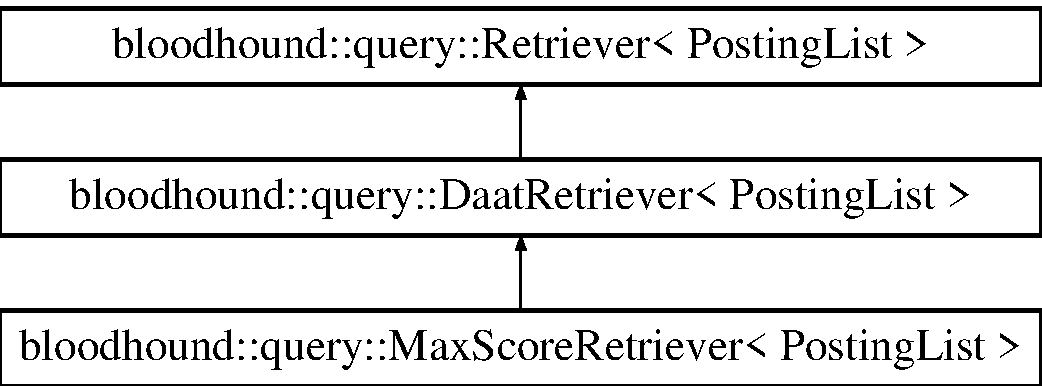
\includegraphics[height=3.000000cm]{classbloodhound_1_1query_1_1MaxScoreRetriever}
\end{center}
\end{figure}
\subsection*{Additional Inherited Members}


The documentation for this class was generated from the following file\+:\begin{DoxyCompactItemize}
\item 
include/\hyperlink{retrievers_8hpp}{retrievers.\+hpp}\end{DoxyCompactItemize}

\hypertarget{structirkit_1_1moving__range}{}\section{irkit\+:\+:moving\+\_\+range$<$ Iter $>$ Struct Template Reference}
\label{structirkit_1_1moving__range}\index{irkit\+::moving\+\_\+range$<$ Iter $>$@{irkit\+::moving\+\_\+range$<$ Iter $>$}}


{\ttfamily \#include $<$daat.\+hpp$>$}

\subsection*{Public Member Functions}
\begin{DoxyCompactItemize}
\item 
\hyperlink{structirkit_1_1moving__range_a9b6d474c670875034ca5a044b0a2fc14}{moving\+\_\+range} ()=default
\item 
\hyperlink{structirkit_1_1moving__range_a79a261cc6e7da7ffb0d93a198fe3dab7}{moving\+\_\+range} (Iter first, Iter last)
\item 
bool \hyperlink{structirkit_1_1moving__range_a8d4e48c5d31fbc158da77eec0c90010e}{empty} () const
\item 
void \hyperlink{structirkit_1_1moving__range_a5ee65e31d2983395c02b724ede47c034}{advance} ()
\item 
void \hyperlink{structirkit_1_1moving__range_a792efd70f3efcb651bff438a0e0814ce}{advance} (unsigned int n)
\item 
Iter \hyperlink{structirkit_1_1moving__range_af58c3dbe1e87c3222ee4a80aa745d9a1}{begin} () const
\item 
Iter \hyperlink{structirkit_1_1moving__range_a5e5ff06f38d6cdba4735e7dd632759ef}{end} () const
\item 
auto \hyperlink{structirkit_1_1moving__range_a4e4c1a83cb13e1ca572275b2c7885aeb}{head} () const
\end{DoxyCompactItemize}
\subsection*{Public Attributes}
\begin{DoxyCompactItemize}
\item 
Iter \hyperlink{structirkit_1_1moving__range_a175a0bc6996715ea27e6b87abff03139}{left}
\item 
Iter \hyperlink{structirkit_1_1moving__range_aa64b16b98bdd7b627ecceb82c8ef3bec}{right}
\end{DoxyCompactItemize}


\subsection{Detailed Description}
\subsubsection*{template$<$class Iter$>$\newline
struct irkit\+::moving\+\_\+range$<$ Iter $>$}

A container for two ends of iterators. T\+O\+DO\+: Needs to be generalized, for containers as well? T\+O\+DO\+: Implement iterator methods. 

\subsection{Constructor \& Destructor Documentation}
\mbox{\Hypertarget{structirkit_1_1moving__range_a9b6d474c670875034ca5a044b0a2fc14}\label{structirkit_1_1moving__range_a9b6d474c670875034ca5a044b0a2fc14}} 
\index{irkit\+::moving\+\_\+range@{irkit\+::moving\+\_\+range}!moving\+\_\+range@{moving\+\_\+range}}
\index{moving\+\_\+range@{moving\+\_\+range}!irkit\+::moving\+\_\+range@{irkit\+::moving\+\_\+range}}
\subsubsection{\texorpdfstring{moving\+\_\+range()}{moving\_range()}\hspace{0.1cm}{\footnotesize\ttfamily [1/2]}}
{\footnotesize\ttfamily template$<$class Iter $>$ \\
\hyperlink{structirkit_1_1moving__range}{irkit\+::moving\+\_\+range}$<$ Iter $>$\+::\hyperlink{structirkit_1_1moving__range}{moving\+\_\+range} (\begin{DoxyParamCaption}{ }\end{DoxyParamCaption})\hspace{0.3cm}{\ttfamily [default]}}

\mbox{\Hypertarget{structirkit_1_1moving__range_a79a261cc6e7da7ffb0d93a198fe3dab7}\label{structirkit_1_1moving__range_a79a261cc6e7da7ffb0d93a198fe3dab7}} 
\index{irkit\+::moving\+\_\+range@{irkit\+::moving\+\_\+range}!moving\+\_\+range@{moving\+\_\+range}}
\index{moving\+\_\+range@{moving\+\_\+range}!irkit\+::moving\+\_\+range@{irkit\+::moving\+\_\+range}}
\subsubsection{\texorpdfstring{moving\+\_\+range()}{moving\_range()}\hspace{0.1cm}{\footnotesize\ttfamily [2/2]}}
{\footnotesize\ttfamily template$<$class Iter $>$ \\
\hyperlink{structirkit_1_1moving__range}{irkit\+::moving\+\_\+range}$<$ Iter $>$\+::\hyperlink{structirkit_1_1moving__range}{moving\+\_\+range} (\begin{DoxyParamCaption}\item[{Iter}]{first,  }\item[{Iter}]{last }\end{DoxyParamCaption})\hspace{0.3cm}{\ttfamily [inline]}}



\subsection{Member Function Documentation}
\mbox{\Hypertarget{structirkit_1_1moving__range_a5ee65e31d2983395c02b724ede47c034}\label{structirkit_1_1moving__range_a5ee65e31d2983395c02b724ede47c034}} 
\index{irkit\+::moving\+\_\+range@{irkit\+::moving\+\_\+range}!advance@{advance}}
\index{advance@{advance}!irkit\+::moving\+\_\+range@{irkit\+::moving\+\_\+range}}
\subsubsection{\texorpdfstring{advance()}{advance()}\hspace{0.1cm}{\footnotesize\ttfamily [1/2]}}
{\footnotesize\ttfamily template$<$class Iter $>$ \\
void \hyperlink{structirkit_1_1moving__range}{irkit\+::moving\+\_\+range}$<$ Iter $>$\+::advance (\begin{DoxyParamCaption}{ }\end{DoxyParamCaption})\hspace{0.3cm}{\ttfamily [inline]}}

\mbox{\Hypertarget{structirkit_1_1moving__range_a792efd70f3efcb651bff438a0e0814ce}\label{structirkit_1_1moving__range_a792efd70f3efcb651bff438a0e0814ce}} 
\index{irkit\+::moving\+\_\+range@{irkit\+::moving\+\_\+range}!advance@{advance}}
\index{advance@{advance}!irkit\+::moving\+\_\+range@{irkit\+::moving\+\_\+range}}
\subsubsection{\texorpdfstring{advance()}{advance()}\hspace{0.1cm}{\footnotesize\ttfamily [2/2]}}
{\footnotesize\ttfamily template$<$class Iter $>$ \\
void \hyperlink{structirkit_1_1moving__range}{irkit\+::moving\+\_\+range}$<$ Iter $>$\+::advance (\begin{DoxyParamCaption}\item[{unsigned int}]{n }\end{DoxyParamCaption})\hspace{0.3cm}{\ttfamily [inline]}}

\mbox{\Hypertarget{structirkit_1_1moving__range_af58c3dbe1e87c3222ee4a80aa745d9a1}\label{structirkit_1_1moving__range_af58c3dbe1e87c3222ee4a80aa745d9a1}} 
\index{irkit\+::moving\+\_\+range@{irkit\+::moving\+\_\+range}!begin@{begin}}
\index{begin@{begin}!irkit\+::moving\+\_\+range@{irkit\+::moving\+\_\+range}}
\subsubsection{\texorpdfstring{begin()}{begin()}}
{\footnotesize\ttfamily template$<$class Iter $>$ \\
Iter \hyperlink{structirkit_1_1moving__range}{irkit\+::moving\+\_\+range}$<$ Iter $>$\+::begin (\begin{DoxyParamCaption}{ }\end{DoxyParamCaption}) const\hspace{0.3cm}{\ttfamily [inline]}}

\mbox{\Hypertarget{structirkit_1_1moving__range_a8d4e48c5d31fbc158da77eec0c90010e}\label{structirkit_1_1moving__range_a8d4e48c5d31fbc158da77eec0c90010e}} 
\index{irkit\+::moving\+\_\+range@{irkit\+::moving\+\_\+range}!empty@{empty}}
\index{empty@{empty}!irkit\+::moving\+\_\+range@{irkit\+::moving\+\_\+range}}
\subsubsection{\texorpdfstring{empty()}{empty()}}
{\footnotesize\ttfamily template$<$class Iter $>$ \\
bool \hyperlink{structirkit_1_1moving__range}{irkit\+::moving\+\_\+range}$<$ Iter $>$\+::empty (\begin{DoxyParamCaption}{ }\end{DoxyParamCaption}) const\hspace{0.3cm}{\ttfamily [inline]}}

\mbox{\Hypertarget{structirkit_1_1moving__range_a5e5ff06f38d6cdba4735e7dd632759ef}\label{structirkit_1_1moving__range_a5e5ff06f38d6cdba4735e7dd632759ef}} 
\index{irkit\+::moving\+\_\+range@{irkit\+::moving\+\_\+range}!end@{end}}
\index{end@{end}!irkit\+::moving\+\_\+range@{irkit\+::moving\+\_\+range}}
\subsubsection{\texorpdfstring{end()}{end()}}
{\footnotesize\ttfamily template$<$class Iter $>$ \\
Iter \hyperlink{structirkit_1_1moving__range}{irkit\+::moving\+\_\+range}$<$ Iter $>$\+::end (\begin{DoxyParamCaption}{ }\end{DoxyParamCaption}) const\hspace{0.3cm}{\ttfamily [inline]}}

\mbox{\Hypertarget{structirkit_1_1moving__range_a4e4c1a83cb13e1ca572275b2c7885aeb}\label{structirkit_1_1moving__range_a4e4c1a83cb13e1ca572275b2c7885aeb}} 
\index{irkit\+::moving\+\_\+range@{irkit\+::moving\+\_\+range}!head@{head}}
\index{head@{head}!irkit\+::moving\+\_\+range@{irkit\+::moving\+\_\+range}}
\subsubsection{\texorpdfstring{head()}{head()}}
{\footnotesize\ttfamily template$<$class Iter $>$ \\
auto \hyperlink{structirkit_1_1moving__range}{irkit\+::moving\+\_\+range}$<$ Iter $>$\+::head (\begin{DoxyParamCaption}{ }\end{DoxyParamCaption}) const\hspace{0.3cm}{\ttfamily [inline]}}



\subsection{Member Data Documentation}
\mbox{\Hypertarget{structirkit_1_1moving__range_a175a0bc6996715ea27e6b87abff03139}\label{structirkit_1_1moving__range_a175a0bc6996715ea27e6b87abff03139}} 
\index{irkit\+::moving\+\_\+range@{irkit\+::moving\+\_\+range}!left@{left}}
\index{left@{left}!irkit\+::moving\+\_\+range@{irkit\+::moving\+\_\+range}}
\subsubsection{\texorpdfstring{left}{left}}
{\footnotesize\ttfamily template$<$class Iter $>$ \\
Iter \hyperlink{structirkit_1_1moving__range}{irkit\+::moving\+\_\+range}$<$ Iter $>$\+::left}

\mbox{\Hypertarget{structirkit_1_1moving__range_aa64b16b98bdd7b627ecceb82c8ef3bec}\label{structirkit_1_1moving__range_aa64b16b98bdd7b627ecceb82c8ef3bec}} 
\index{irkit\+::moving\+\_\+range@{irkit\+::moving\+\_\+range}!right@{right}}
\index{right@{right}!irkit\+::moving\+\_\+range@{irkit\+::moving\+\_\+range}}
\subsubsection{\texorpdfstring{right}{right}}
{\footnotesize\ttfamily template$<$class Iter $>$ \\
Iter \hyperlink{structirkit_1_1moving__range}{irkit\+::moving\+\_\+range}$<$ Iter $>$\+::right}



The documentation for this struct was generated from the following file\+:\begin{DoxyCompactItemize}
\item 
include/irkit/\hyperlink{daat_8hpp}{daat.\+hpp}\end{DoxyCompactItemize}

\hypertarget{structbloodhound_1_1Offset}{}\section{bloodhound\+:\+:Offset Struct Reference}
\label{structbloodhound_1_1Offset}\index{bloodhound\+::\+Offset@{bloodhound\+::\+Offset}}


{\ttfamily \#include $<$index.\+hpp$>$}

Inheritance diagram for bloodhound\+:\+:Offset\+:\begin{figure}[H]
\begin{center}
\leavevmode
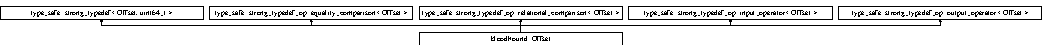
\includegraphics[height=0.598930cm]{structbloodhound_1_1Offset}
\end{center}
\end{figure}
\subsection*{Friends}
\begin{DoxyCompactItemize}
\item 
const char $\ast$ \mbox{\hyperlink{structbloodhound_1_1Offset_aaed86d39530be98502fa1560b323d07b}{operator+}} (const char $\ast$ptr, \mbox{\hyperlink{structbloodhound_1_1Offset}{Offset}} offset)
\item 
char $\ast$ \mbox{\hyperlink{structbloodhound_1_1Offset_aec6c323c060e7a7cae481422f1ecea7a}{operator+}} (char $\ast$ptr, \mbox{\hyperlink{structbloodhound_1_1Offset}{Offset}} offset)
\end{DoxyCompactItemize}


\subsection{Friends And Related Function Documentation}
\mbox{\Hypertarget{structbloodhound_1_1Offset_aaed86d39530be98502fa1560b323d07b}\label{structbloodhound_1_1Offset_aaed86d39530be98502fa1560b323d07b}} 
\index{bloodhound\+::\+Offset@{bloodhound\+::\+Offset}!operator+@{operator+}}
\index{operator+@{operator+}!bloodhound\+::\+Offset@{bloodhound\+::\+Offset}}
\subsubsection{\texorpdfstring{operator+}{operator+}\hspace{0.1cm}{\footnotesize\ttfamily [1/2]}}
{\footnotesize\ttfamily const char$\ast$ operator+ (\begin{DoxyParamCaption}\item[{const char $\ast$}]{ptr,  }\item[{\mbox{\hyperlink{structbloodhound_1_1Offset}{Offset}}}]{offset }\end{DoxyParamCaption})\hspace{0.3cm}{\ttfamily [friend]}}

\mbox{\Hypertarget{structbloodhound_1_1Offset_aec6c323c060e7a7cae481422f1ecea7a}\label{structbloodhound_1_1Offset_aec6c323c060e7a7cae481422f1ecea7a}} 
\index{bloodhound\+::\+Offset@{bloodhound\+::\+Offset}!operator+@{operator+}}
\index{operator+@{operator+}!bloodhound\+::\+Offset@{bloodhound\+::\+Offset}}
\subsubsection{\texorpdfstring{operator+}{operator+}\hspace{0.1cm}{\footnotesize\ttfamily [2/2]}}
{\footnotesize\ttfamily char$\ast$ operator+ (\begin{DoxyParamCaption}\item[{char $\ast$}]{ptr,  }\item[{\mbox{\hyperlink{structbloodhound_1_1Offset}{Offset}}}]{offset }\end{DoxyParamCaption})\hspace{0.3cm}{\ttfamily [friend]}}



The documentation for this struct was generated from the following file\+:\begin{DoxyCompactItemize}
\item 
include/\mbox{\hyperlink{index_8hpp}{index.\+hpp}}\end{DoxyCompactItemize}

\hypertarget{structbloodhound_1_1Posting}{}\section{bloodhound\+:\+:Posting Struct Reference}
\label{structbloodhound_1_1Posting}\index{bloodhound\+::\+Posting@{bloodhound\+::\+Posting}}


{\ttfamily \#include $<$index.\+hpp$>$}

\subsection*{Public Attributes}
\begin{DoxyCompactItemize}
\item 
\mbox{\hyperlink{structbloodhound_1_1Doc}{Doc}} \mbox{\hyperlink{structbloodhound_1_1Posting_ae39f120507b708385e754c693109e384}{doc}}
\item 
\mbox{\hyperlink{structbloodhound_1_1Score}{Score}} \mbox{\hyperlink{structbloodhound_1_1Posting_afcdc4c2d2486c04feee39077122e1622}{score}}
\end{DoxyCompactItemize}


\subsection{Member Data Documentation}
\mbox{\Hypertarget{structbloodhound_1_1Posting_ae39f120507b708385e754c693109e384}\label{structbloodhound_1_1Posting_ae39f120507b708385e754c693109e384}} 
\index{bloodhound\+::\+Posting@{bloodhound\+::\+Posting}!doc@{doc}}
\index{doc@{doc}!bloodhound\+::\+Posting@{bloodhound\+::\+Posting}}
\subsubsection{\texorpdfstring{doc}{doc}}
{\footnotesize\ttfamily \mbox{\hyperlink{structbloodhound_1_1Doc}{Doc}} bloodhound\+::\+Posting\+::doc}

\mbox{\Hypertarget{structbloodhound_1_1Posting_afcdc4c2d2486c04feee39077122e1622}\label{structbloodhound_1_1Posting_afcdc4c2d2486c04feee39077122e1622}} 
\index{bloodhound\+::\+Posting@{bloodhound\+::\+Posting}!score@{score}}
\index{score@{score}!bloodhound\+::\+Posting@{bloodhound\+::\+Posting}}
\subsubsection{\texorpdfstring{score}{score}}
{\footnotesize\ttfamily \mbox{\hyperlink{structbloodhound_1_1Score}{Score}} bloodhound\+::\+Posting\+::score}



The documentation for this struct was generated from the following file\+:\begin{DoxyCompactItemize}
\item 
include/\mbox{\hyperlink{index_8hpp}{index.\+hpp}}\end{DoxyCompactItemize}

\hypertarget{structbloodhound_1_1index_1_1format_1_1PostingBlock}{}\section{bloodhound\+:\+:index\+:\+:format\+:\+:Posting\+Block$<$ Value $>$ Struct Template Reference}
\label{structbloodhound_1_1index_1_1format_1_1PostingBlock}\index{bloodhound\+::index\+::format\+::\+Posting\+Block$<$ Value $>$@{bloodhound\+::index\+::format\+::\+Posting\+Block$<$ Value $>$}}


{\ttfamily \#include $<$format.\+hpp$>$}

\subsection*{Public Attributes}
\begin{DoxyCompactItemize}
\item 
Value \mbox{\hyperlink{structbloodhound_1_1index_1_1format_1_1PostingBlock_a0820d9474f2563bf913457e3b8681370}{head}}
\item 
\mbox{\hyperlink{structbloodhound_1_1RelativeOffset}{Relative\+Offset}} \mbox{\hyperlink{structbloodhound_1_1index_1_1format_1_1PostingBlock_ad7e7da1b1f4ed16a0b51ba9c8fbac401}{next\+\_\+block}}
\end{DoxyCompactItemize}


\subsection{Member Data Documentation}
\mbox{\Hypertarget{structbloodhound_1_1index_1_1format_1_1PostingBlock_a0820d9474f2563bf913457e3b8681370}\label{structbloodhound_1_1index_1_1format_1_1PostingBlock_a0820d9474f2563bf913457e3b8681370}} 
\index{bloodhound\+::index\+::format\+::\+Posting\+Block@{bloodhound\+::index\+::format\+::\+Posting\+Block}!head@{head}}
\index{head@{head}!bloodhound\+::index\+::format\+::\+Posting\+Block@{bloodhound\+::index\+::format\+::\+Posting\+Block}}
\subsubsection{\texorpdfstring{head}{head}}
{\footnotesize\ttfamily template$<$typename Value $>$ \\
Value \mbox{\hyperlink{structbloodhound_1_1index_1_1format_1_1PostingBlock}{bloodhound\+::index\+::format\+::\+Posting\+Block}}$<$ Value $>$\+::head}

\mbox{\Hypertarget{structbloodhound_1_1index_1_1format_1_1PostingBlock_ad7e7da1b1f4ed16a0b51ba9c8fbac401}\label{structbloodhound_1_1index_1_1format_1_1PostingBlock_ad7e7da1b1f4ed16a0b51ba9c8fbac401}} 
\index{bloodhound\+::index\+::format\+::\+Posting\+Block@{bloodhound\+::index\+::format\+::\+Posting\+Block}!next\+\_\+block@{next\+\_\+block}}
\index{next\+\_\+block@{next\+\_\+block}!bloodhound\+::index\+::format\+::\+Posting\+Block@{bloodhound\+::index\+::format\+::\+Posting\+Block}}
\subsubsection{\texorpdfstring{next\+\_\+block}{next\_block}}
{\footnotesize\ttfamily template$<$typename Value $>$ \\
\mbox{\hyperlink{structbloodhound_1_1RelativeOffset}{Relative\+Offset}} \mbox{\hyperlink{structbloodhound_1_1index_1_1format_1_1PostingBlock}{bloodhound\+::index\+::format\+::\+Posting\+Block}}$<$ Value $>$\+::next\+\_\+block}



The documentation for this struct was generated from the following file\+:\begin{DoxyCompactItemize}
\item 
include/index/\mbox{\hyperlink{format_8hpp}{format.\+hpp}}\end{DoxyCompactItemize}

\hypertarget{classbloodhound_1_1PostingList}{}\section{bloodhound\+:\+:Posting\+List Class Reference}
\label{classbloodhound_1_1PostingList}\index{bloodhound\+::\+Posting\+List@{bloodhound\+::\+Posting\+List}}


{\ttfamily \#include $<$index.\+hpp$>$}

\subsection*{Classes}
\begin{DoxyCompactItemize}
\item 
struct \mbox{\hyperlink{structbloodhound_1_1PostingList_1_1const__iterator}{const\+\_\+iterator}}
\item 
struct \mbox{\hyperlink{structbloodhound_1_1PostingList_1_1iterator}{iterator}}
\end{DoxyCompactItemize}
\subsection*{Public Member Functions}
\begin{DoxyCompactItemize}
\item 
\mbox{\hyperlink{classbloodhound_1_1PostingList_a725f1df76c8278f1d927fff3ed4c496e}{Posting\+List}} (\mbox{\hyperlink{structbloodhound_1_1Doc}{Doc}} $\ast$d, \mbox{\hyperlink{structbloodhound_1_1Score}{Score}} $\ast$s, uint32\+\_\+t l, \mbox{\hyperlink{structbloodhound_1_1Score}{Score}} ms)
\item 
std\+::size\+\_\+t \mbox{\hyperlink{classbloodhound_1_1PostingList_a7af6f4e9fc277dd7c1dc73c2922ceacd}{length}} () const
\item 
std\+::size\+\_\+t \mbox{\hyperlink{classbloodhound_1_1PostingList_a440e43337385c66edb4e1c0568c74544}{size}} () const
\item 
bool \mbox{\hyperlink{classbloodhound_1_1PostingList_a28ec60331aec6acaa9c281d4d412bf26}{empty}} () const
\item 
\mbox{\hyperlink{structbloodhound_1_1PostingList_1_1iterator}{iterator}} \mbox{\hyperlink{classbloodhound_1_1PostingList_abd082192a0339062d318de73c95f1ee5}{next\+\_\+ge}} (\mbox{\hyperlink{structbloodhound_1_1PostingList_1_1iterator}{iterator}} current, \mbox{\hyperlink{structbloodhound_1_1Doc}{Doc}} doc) const
\item 
\mbox{\hyperlink{structbloodhound_1_1PostingList_1_1iterator}{iterator}} \mbox{\hyperlink{classbloodhound_1_1PostingList_aae5c35208d6fb36f611f952ba57add0f}{next\+\_\+ge}} (\mbox{\hyperlink{structbloodhound_1_1PostingList_1_1iterator}{iterator}} current, \mbox{\hyperlink{structbloodhound_1_1PostingList_1_1iterator}{iterator}} \mbox{\hyperlink{classbloodhound_1_1PostingList_a2e1f899bd04ae64e1318494d358ade94}{end}}, \mbox{\hyperlink{structbloodhound_1_1Doc}{Doc}} doc) const
\item 
virtual \mbox{\hyperlink{structbloodhound_1_1PostingList_1_1iterator}{iterator}} \mbox{\hyperlink{classbloodhound_1_1PostingList_a274f57f133cd6763e0d8cc3e00fa1be3}{begin}} () const
\item 
virtual \mbox{\hyperlink{structbloodhound_1_1PostingList_1_1iterator}{iterator}} \mbox{\hyperlink{classbloodhound_1_1PostingList_a2e1f899bd04ae64e1318494d358ade94}{end}} () const
\item 
virtual \mbox{\hyperlink{structbloodhound_1_1PostingList_1_1const__iterator}{const\+\_\+iterator}} \mbox{\hyperlink{classbloodhound_1_1PostingList_a44980317210bfe6c9f7d59dbea1cbd4a}{cbegin}} () const
\item 
virtual \mbox{\hyperlink{structbloodhound_1_1PostingList_1_1const__iterator}{const\+\_\+iterator}} \mbox{\hyperlink{classbloodhound_1_1PostingList_a7eca0ae1f54ddc48757a4fb3c0b885ce}{cend}} () const
\item 
virtual gsl\+::span$<$ \mbox{\hyperlink{structbloodhound_1_1Doc}{Doc}} $>$\+::\mbox{\hyperlink{structbloodhound_1_1PostingList_1_1const__iterator}{const\+\_\+iterator}} \mbox{\hyperlink{classbloodhound_1_1PostingList_aac3dbe7fbf43ce93031e97b16bcfc888}{doc\+\_\+begin}} () const
\item 
virtual gsl\+::span$<$ \mbox{\hyperlink{structbloodhound_1_1Doc}{Doc}} $>$\+::\mbox{\hyperlink{structbloodhound_1_1PostingList_1_1const__iterator}{const\+\_\+iterator}} \mbox{\hyperlink{classbloodhound_1_1PostingList_aac468540b0a376d9b378a4333546245c}{doc\+\_\+end}} () const
\item 
virtual gsl\+::span$<$ \mbox{\hyperlink{structbloodhound_1_1Score}{Score}} $>$\+::\mbox{\hyperlink{structbloodhound_1_1PostingList_1_1const__iterator}{const\+\_\+iterator}} \mbox{\hyperlink{classbloodhound_1_1PostingList_aec5d5bb81622fb64d7b64416a8491456}{score\+\_\+begin}} () const
\item 
virtual gsl\+::span$<$ \mbox{\hyperlink{structbloodhound_1_1Score}{Score}} $>$\+::\mbox{\hyperlink{structbloodhound_1_1PostingList_1_1const__iterator}{const\+\_\+iterator}} \mbox{\hyperlink{classbloodhound_1_1PostingList_ae89abf9882f73f35a6e106c5a328ca6f}{score\+\_\+end}} () const
\item 
void \mbox{\hyperlink{classbloodhound_1_1PostingList_a3c9d6c5e88a7aae2642ff1d0f52160c0}{make\+\_\+et}} (double et\+\_\+threshold)
\item 
\mbox{\hyperlink{structbloodhound_1_1Doc}{Doc}} $\ast$ \mbox{\hyperlink{classbloodhound_1_1PostingList_acfca9e8ad1fd94461b56390fdd60779f}{docs\+\_\+ptr}} () const
\item 
\mbox{\hyperlink{structbloodhound_1_1Score}{Score}} $\ast$ \mbox{\hyperlink{classbloodhound_1_1PostingList_a79be9c874bb91e17ca308ae0528e9277}{scores\+\_\+ptr}} () const
\end{DoxyCompactItemize}
\subsection*{Public Attributes}
\begin{DoxyCompactItemize}
\item 
gsl\+::span$<$ \mbox{\hyperlink{structbloodhound_1_1Doc}{Doc}} $>$ \mbox{\hyperlink{classbloodhound_1_1PostingList_a11749c12634d86c73b7d9c150acaac03}{docs}}
\item 
gsl\+::span$<$ \mbox{\hyperlink{structbloodhound_1_1Score}{Score}} $>$ \mbox{\hyperlink{classbloodhound_1_1PostingList_a2c773bffa3d78d2e7a7e04d918b064da}{scores}}
\item 
\mbox{\hyperlink{structbloodhound_1_1Score}{Score}} \mbox{\hyperlink{classbloodhound_1_1PostingList_ab840a6f9ddf8de353cbdd09b3a184bfa}{max\+\_\+score}}
\item 
std\+::size\+\_\+t \mbox{\hyperlink{classbloodhound_1_1PostingList_a9aa9a9d1db46c6858fa952a36e1bf8fa}{idx}}
\item 
std\+::size\+\_\+t \mbox{\hyperlink{classbloodhound_1_1PostingList_a7c4d53dfa824951670d68ef57cd2068d}{end\+\_\+idx}}
\end{DoxyCompactItemize}


\subsection{Constructor \& Destructor Documentation}
\mbox{\Hypertarget{classbloodhound_1_1PostingList_a725f1df76c8278f1d927fff3ed4c496e}\label{classbloodhound_1_1PostingList_a725f1df76c8278f1d927fff3ed4c496e}} 
\index{bloodhound\+::\+Posting\+List@{bloodhound\+::\+Posting\+List}!Posting\+List@{Posting\+List}}
\index{Posting\+List@{Posting\+List}!bloodhound\+::\+Posting\+List@{bloodhound\+::\+Posting\+List}}
\subsubsection{\texorpdfstring{Posting\+List()}{PostingList()}}
{\footnotesize\ttfamily bloodhound\+::\+Posting\+List\+::\+Posting\+List (\begin{DoxyParamCaption}\item[{\mbox{\hyperlink{structbloodhound_1_1Doc}{Doc}} $\ast$}]{d,  }\item[{\mbox{\hyperlink{structbloodhound_1_1Score}{Score}} $\ast$}]{s,  }\item[{uint32\+\_\+t}]{l,  }\item[{\mbox{\hyperlink{structbloodhound_1_1Score}{Score}}}]{ms }\end{DoxyParamCaption})\hspace{0.3cm}{\ttfamily [inline]}}



\subsection{Member Function Documentation}
\mbox{\Hypertarget{classbloodhound_1_1PostingList_a274f57f133cd6763e0d8cc3e00fa1be3}\label{classbloodhound_1_1PostingList_a274f57f133cd6763e0d8cc3e00fa1be3}} 
\index{bloodhound\+::\+Posting\+List@{bloodhound\+::\+Posting\+List}!begin@{begin}}
\index{begin@{begin}!bloodhound\+::\+Posting\+List@{bloodhound\+::\+Posting\+List}}
\subsubsection{\texorpdfstring{begin()}{begin()}}
{\footnotesize\ttfamily virtual \mbox{\hyperlink{structbloodhound_1_1PostingList_1_1iterator}{iterator}} bloodhound\+::\+Posting\+List\+::begin (\begin{DoxyParamCaption}{ }\end{DoxyParamCaption}) const\hspace{0.3cm}{\ttfamily [inline]}, {\ttfamily [virtual]}}

\mbox{\Hypertarget{classbloodhound_1_1PostingList_a44980317210bfe6c9f7d59dbea1cbd4a}\label{classbloodhound_1_1PostingList_a44980317210bfe6c9f7d59dbea1cbd4a}} 
\index{bloodhound\+::\+Posting\+List@{bloodhound\+::\+Posting\+List}!cbegin@{cbegin}}
\index{cbegin@{cbegin}!bloodhound\+::\+Posting\+List@{bloodhound\+::\+Posting\+List}}
\subsubsection{\texorpdfstring{cbegin()}{cbegin()}}
{\footnotesize\ttfamily virtual \mbox{\hyperlink{structbloodhound_1_1PostingList_1_1const__iterator}{const\+\_\+iterator}} bloodhound\+::\+Posting\+List\+::cbegin (\begin{DoxyParamCaption}{ }\end{DoxyParamCaption}) const\hspace{0.3cm}{\ttfamily [inline]}, {\ttfamily [virtual]}}

\mbox{\Hypertarget{classbloodhound_1_1PostingList_a7eca0ae1f54ddc48757a4fb3c0b885ce}\label{classbloodhound_1_1PostingList_a7eca0ae1f54ddc48757a4fb3c0b885ce}} 
\index{bloodhound\+::\+Posting\+List@{bloodhound\+::\+Posting\+List}!cend@{cend}}
\index{cend@{cend}!bloodhound\+::\+Posting\+List@{bloodhound\+::\+Posting\+List}}
\subsubsection{\texorpdfstring{cend()}{cend()}}
{\footnotesize\ttfamily virtual \mbox{\hyperlink{structbloodhound_1_1PostingList_1_1const__iterator}{const\+\_\+iterator}} bloodhound\+::\+Posting\+List\+::cend (\begin{DoxyParamCaption}{ }\end{DoxyParamCaption}) const\hspace{0.3cm}{\ttfamily [inline]}, {\ttfamily [virtual]}}

\mbox{\Hypertarget{classbloodhound_1_1PostingList_aac3dbe7fbf43ce93031e97b16bcfc888}\label{classbloodhound_1_1PostingList_aac3dbe7fbf43ce93031e97b16bcfc888}} 
\index{bloodhound\+::\+Posting\+List@{bloodhound\+::\+Posting\+List}!doc\+\_\+begin@{doc\+\_\+begin}}
\index{doc\+\_\+begin@{doc\+\_\+begin}!bloodhound\+::\+Posting\+List@{bloodhound\+::\+Posting\+List}}
\subsubsection{\texorpdfstring{doc\+\_\+begin()}{doc\_begin()}}
{\footnotesize\ttfamily virtual gsl\+::span$<$\mbox{\hyperlink{structbloodhound_1_1Doc}{Doc}}$>$\+::\mbox{\hyperlink{structbloodhound_1_1PostingList_1_1const__iterator}{const\+\_\+iterator}} bloodhound\+::\+Posting\+List\+::doc\+\_\+begin (\begin{DoxyParamCaption}{ }\end{DoxyParamCaption}) const\hspace{0.3cm}{\ttfamily [inline]}, {\ttfamily [virtual]}}

\mbox{\Hypertarget{classbloodhound_1_1PostingList_aac468540b0a376d9b378a4333546245c}\label{classbloodhound_1_1PostingList_aac468540b0a376d9b378a4333546245c}} 
\index{bloodhound\+::\+Posting\+List@{bloodhound\+::\+Posting\+List}!doc\+\_\+end@{doc\+\_\+end}}
\index{doc\+\_\+end@{doc\+\_\+end}!bloodhound\+::\+Posting\+List@{bloodhound\+::\+Posting\+List}}
\subsubsection{\texorpdfstring{doc\+\_\+end()}{doc\_end()}}
{\footnotesize\ttfamily virtual gsl\+::span$<$\mbox{\hyperlink{structbloodhound_1_1Doc}{Doc}}$>$\+::\mbox{\hyperlink{structbloodhound_1_1PostingList_1_1const__iterator}{const\+\_\+iterator}} bloodhound\+::\+Posting\+List\+::doc\+\_\+end (\begin{DoxyParamCaption}{ }\end{DoxyParamCaption}) const\hspace{0.3cm}{\ttfamily [inline]}, {\ttfamily [virtual]}}

\mbox{\Hypertarget{classbloodhound_1_1PostingList_acfca9e8ad1fd94461b56390fdd60779f}\label{classbloodhound_1_1PostingList_acfca9e8ad1fd94461b56390fdd60779f}} 
\index{bloodhound\+::\+Posting\+List@{bloodhound\+::\+Posting\+List}!docs\+\_\+ptr@{docs\+\_\+ptr}}
\index{docs\+\_\+ptr@{docs\+\_\+ptr}!bloodhound\+::\+Posting\+List@{bloodhound\+::\+Posting\+List}}
\subsubsection{\texorpdfstring{docs\+\_\+ptr()}{docs\_ptr()}}
{\footnotesize\ttfamily \mbox{\hyperlink{structbloodhound_1_1Doc}{Doc}}$\ast$ bloodhound\+::\+Posting\+List\+::docs\+\_\+ptr (\begin{DoxyParamCaption}{ }\end{DoxyParamCaption}) const\hspace{0.3cm}{\ttfamily [inline]}}

\mbox{\Hypertarget{classbloodhound_1_1PostingList_a28ec60331aec6acaa9c281d4d412bf26}\label{classbloodhound_1_1PostingList_a28ec60331aec6acaa9c281d4d412bf26}} 
\index{bloodhound\+::\+Posting\+List@{bloodhound\+::\+Posting\+List}!empty@{empty}}
\index{empty@{empty}!bloodhound\+::\+Posting\+List@{bloodhound\+::\+Posting\+List}}
\subsubsection{\texorpdfstring{empty()}{empty()}}
{\footnotesize\ttfamily bool bloodhound\+::\+Posting\+List\+::empty (\begin{DoxyParamCaption}{ }\end{DoxyParamCaption}) const\hspace{0.3cm}{\ttfamily [inline]}}

\mbox{\Hypertarget{classbloodhound_1_1PostingList_a2e1f899bd04ae64e1318494d358ade94}\label{classbloodhound_1_1PostingList_a2e1f899bd04ae64e1318494d358ade94}} 
\index{bloodhound\+::\+Posting\+List@{bloodhound\+::\+Posting\+List}!end@{end}}
\index{end@{end}!bloodhound\+::\+Posting\+List@{bloodhound\+::\+Posting\+List}}
\subsubsection{\texorpdfstring{end()}{end()}}
{\footnotesize\ttfamily virtual \mbox{\hyperlink{structbloodhound_1_1PostingList_1_1iterator}{iterator}} bloodhound\+::\+Posting\+List\+::end (\begin{DoxyParamCaption}{ }\end{DoxyParamCaption}) const\hspace{0.3cm}{\ttfamily [inline]}, {\ttfamily [virtual]}}

\mbox{\Hypertarget{classbloodhound_1_1PostingList_a7af6f4e9fc277dd7c1dc73c2922ceacd}\label{classbloodhound_1_1PostingList_a7af6f4e9fc277dd7c1dc73c2922ceacd}} 
\index{bloodhound\+::\+Posting\+List@{bloodhound\+::\+Posting\+List}!length@{length}}
\index{length@{length}!bloodhound\+::\+Posting\+List@{bloodhound\+::\+Posting\+List}}
\subsubsection{\texorpdfstring{length()}{length()}}
{\footnotesize\ttfamily std\+::size\+\_\+t bloodhound\+::\+Posting\+List\+::length (\begin{DoxyParamCaption}{ }\end{DoxyParamCaption}) const\hspace{0.3cm}{\ttfamily [inline]}}

\mbox{\Hypertarget{classbloodhound_1_1PostingList_a3c9d6c5e88a7aae2642ff1d0f52160c0}\label{classbloodhound_1_1PostingList_a3c9d6c5e88a7aae2642ff1d0f52160c0}} 
\index{bloodhound\+::\+Posting\+List@{bloodhound\+::\+Posting\+List}!make\+\_\+et@{make\+\_\+et}}
\index{make\+\_\+et@{make\+\_\+et}!bloodhound\+::\+Posting\+List@{bloodhound\+::\+Posting\+List}}
\subsubsection{\texorpdfstring{make\+\_\+et()}{make\_et()}}
{\footnotesize\ttfamily void bloodhound\+::\+Posting\+List\+::make\+\_\+et (\begin{DoxyParamCaption}\item[{double}]{et\+\_\+threshold }\end{DoxyParamCaption})\hspace{0.3cm}{\ttfamily [inline]}}

\mbox{\Hypertarget{classbloodhound_1_1PostingList_abd082192a0339062d318de73c95f1ee5}\label{classbloodhound_1_1PostingList_abd082192a0339062d318de73c95f1ee5}} 
\index{bloodhound\+::\+Posting\+List@{bloodhound\+::\+Posting\+List}!next\+\_\+ge@{next\+\_\+ge}}
\index{next\+\_\+ge@{next\+\_\+ge}!bloodhound\+::\+Posting\+List@{bloodhound\+::\+Posting\+List}}
\subsubsection{\texorpdfstring{next\+\_\+ge()}{next\_ge()}\hspace{0.1cm}{\footnotesize\ttfamily [1/2]}}
{\footnotesize\ttfamily \mbox{\hyperlink{structbloodhound_1_1PostingList_1_1iterator}{iterator}} bloodhound\+::\+Posting\+List\+::next\+\_\+ge (\begin{DoxyParamCaption}\item[{\mbox{\hyperlink{structbloodhound_1_1PostingList_1_1iterator}{iterator}}}]{current,  }\item[{\mbox{\hyperlink{structbloodhound_1_1Doc}{Doc}}}]{doc }\end{DoxyParamCaption}) const\hspace{0.3cm}{\ttfamily [inline]}}

\mbox{\Hypertarget{classbloodhound_1_1PostingList_aae5c35208d6fb36f611f952ba57add0f}\label{classbloodhound_1_1PostingList_aae5c35208d6fb36f611f952ba57add0f}} 
\index{bloodhound\+::\+Posting\+List@{bloodhound\+::\+Posting\+List}!next\+\_\+ge@{next\+\_\+ge}}
\index{next\+\_\+ge@{next\+\_\+ge}!bloodhound\+::\+Posting\+List@{bloodhound\+::\+Posting\+List}}
\subsubsection{\texorpdfstring{next\+\_\+ge()}{next\_ge()}\hspace{0.1cm}{\footnotesize\ttfamily [2/2]}}
{\footnotesize\ttfamily \mbox{\hyperlink{structbloodhound_1_1PostingList_1_1iterator}{iterator}} bloodhound\+::\+Posting\+List\+::next\+\_\+ge (\begin{DoxyParamCaption}\item[{\mbox{\hyperlink{structbloodhound_1_1PostingList_1_1iterator}{iterator}}}]{current,  }\item[{\mbox{\hyperlink{structbloodhound_1_1PostingList_1_1iterator}{iterator}}}]{end,  }\item[{\mbox{\hyperlink{structbloodhound_1_1Doc}{Doc}}}]{doc }\end{DoxyParamCaption}) const\hspace{0.3cm}{\ttfamily [inline]}}

\mbox{\Hypertarget{classbloodhound_1_1PostingList_aec5d5bb81622fb64d7b64416a8491456}\label{classbloodhound_1_1PostingList_aec5d5bb81622fb64d7b64416a8491456}} 
\index{bloodhound\+::\+Posting\+List@{bloodhound\+::\+Posting\+List}!score\+\_\+begin@{score\+\_\+begin}}
\index{score\+\_\+begin@{score\+\_\+begin}!bloodhound\+::\+Posting\+List@{bloodhound\+::\+Posting\+List}}
\subsubsection{\texorpdfstring{score\+\_\+begin()}{score\_begin()}}
{\footnotesize\ttfamily virtual gsl\+::span$<$\mbox{\hyperlink{structbloodhound_1_1Score}{Score}}$>$\+::\mbox{\hyperlink{structbloodhound_1_1PostingList_1_1const__iterator}{const\+\_\+iterator}} bloodhound\+::\+Posting\+List\+::score\+\_\+begin (\begin{DoxyParamCaption}{ }\end{DoxyParamCaption}) const\hspace{0.3cm}{\ttfamily [inline]}, {\ttfamily [virtual]}}

\mbox{\Hypertarget{classbloodhound_1_1PostingList_ae89abf9882f73f35a6e106c5a328ca6f}\label{classbloodhound_1_1PostingList_ae89abf9882f73f35a6e106c5a328ca6f}} 
\index{bloodhound\+::\+Posting\+List@{bloodhound\+::\+Posting\+List}!score\+\_\+end@{score\+\_\+end}}
\index{score\+\_\+end@{score\+\_\+end}!bloodhound\+::\+Posting\+List@{bloodhound\+::\+Posting\+List}}
\subsubsection{\texorpdfstring{score\+\_\+end()}{score\_end()}}
{\footnotesize\ttfamily virtual gsl\+::span$<$\mbox{\hyperlink{structbloodhound_1_1Score}{Score}}$>$\+::\mbox{\hyperlink{structbloodhound_1_1PostingList_1_1const__iterator}{const\+\_\+iterator}} bloodhound\+::\+Posting\+List\+::score\+\_\+end (\begin{DoxyParamCaption}{ }\end{DoxyParamCaption}) const\hspace{0.3cm}{\ttfamily [inline]}, {\ttfamily [virtual]}}

\mbox{\Hypertarget{classbloodhound_1_1PostingList_a79be9c874bb91e17ca308ae0528e9277}\label{classbloodhound_1_1PostingList_a79be9c874bb91e17ca308ae0528e9277}} 
\index{bloodhound\+::\+Posting\+List@{bloodhound\+::\+Posting\+List}!scores\+\_\+ptr@{scores\+\_\+ptr}}
\index{scores\+\_\+ptr@{scores\+\_\+ptr}!bloodhound\+::\+Posting\+List@{bloodhound\+::\+Posting\+List}}
\subsubsection{\texorpdfstring{scores\+\_\+ptr()}{scores\_ptr()}}
{\footnotesize\ttfamily \mbox{\hyperlink{structbloodhound_1_1Score}{Score}}$\ast$ bloodhound\+::\+Posting\+List\+::scores\+\_\+ptr (\begin{DoxyParamCaption}{ }\end{DoxyParamCaption}) const\hspace{0.3cm}{\ttfamily [inline]}}

\mbox{\Hypertarget{classbloodhound_1_1PostingList_a440e43337385c66edb4e1c0568c74544}\label{classbloodhound_1_1PostingList_a440e43337385c66edb4e1c0568c74544}} 
\index{bloodhound\+::\+Posting\+List@{bloodhound\+::\+Posting\+List}!size@{size}}
\index{size@{size}!bloodhound\+::\+Posting\+List@{bloodhound\+::\+Posting\+List}}
\subsubsection{\texorpdfstring{size()}{size()}}
{\footnotesize\ttfamily std\+::size\+\_\+t bloodhound\+::\+Posting\+List\+::size (\begin{DoxyParamCaption}{ }\end{DoxyParamCaption}) const\hspace{0.3cm}{\ttfamily [inline]}}



\subsection{Member Data Documentation}
\mbox{\Hypertarget{classbloodhound_1_1PostingList_a11749c12634d86c73b7d9c150acaac03}\label{classbloodhound_1_1PostingList_a11749c12634d86c73b7d9c150acaac03}} 
\index{bloodhound\+::\+Posting\+List@{bloodhound\+::\+Posting\+List}!docs@{docs}}
\index{docs@{docs}!bloodhound\+::\+Posting\+List@{bloodhound\+::\+Posting\+List}}
\subsubsection{\texorpdfstring{docs}{docs}}
{\footnotesize\ttfamily gsl\+::span$<$\mbox{\hyperlink{structbloodhound_1_1Doc}{Doc}}$>$ bloodhound\+::\+Posting\+List\+::docs}

\mbox{\Hypertarget{classbloodhound_1_1PostingList_a7c4d53dfa824951670d68ef57cd2068d}\label{classbloodhound_1_1PostingList_a7c4d53dfa824951670d68ef57cd2068d}} 
\index{bloodhound\+::\+Posting\+List@{bloodhound\+::\+Posting\+List}!end\+\_\+idx@{end\+\_\+idx}}
\index{end\+\_\+idx@{end\+\_\+idx}!bloodhound\+::\+Posting\+List@{bloodhound\+::\+Posting\+List}}
\subsubsection{\texorpdfstring{end\+\_\+idx}{end\_idx}}
{\footnotesize\ttfamily std\+::size\+\_\+t bloodhound\+::\+Posting\+List\+::end\+\_\+idx}

\mbox{\Hypertarget{classbloodhound_1_1PostingList_a9aa9a9d1db46c6858fa952a36e1bf8fa}\label{classbloodhound_1_1PostingList_a9aa9a9d1db46c6858fa952a36e1bf8fa}} 
\index{bloodhound\+::\+Posting\+List@{bloodhound\+::\+Posting\+List}!idx@{idx}}
\index{idx@{idx}!bloodhound\+::\+Posting\+List@{bloodhound\+::\+Posting\+List}}
\subsubsection{\texorpdfstring{idx}{idx}}
{\footnotesize\ttfamily std\+::size\+\_\+t bloodhound\+::\+Posting\+List\+::idx}

\mbox{\Hypertarget{classbloodhound_1_1PostingList_ab840a6f9ddf8de353cbdd09b3a184bfa}\label{classbloodhound_1_1PostingList_ab840a6f9ddf8de353cbdd09b3a184bfa}} 
\index{bloodhound\+::\+Posting\+List@{bloodhound\+::\+Posting\+List}!max\+\_\+score@{max\+\_\+score}}
\index{max\+\_\+score@{max\+\_\+score}!bloodhound\+::\+Posting\+List@{bloodhound\+::\+Posting\+List}}
\subsubsection{\texorpdfstring{max\+\_\+score}{max\_score}}
{\footnotesize\ttfamily \mbox{\hyperlink{structbloodhound_1_1Score}{Score}} bloodhound\+::\+Posting\+List\+::max\+\_\+score}

\mbox{\Hypertarget{classbloodhound_1_1PostingList_a2c773bffa3d78d2e7a7e04d918b064da}\label{classbloodhound_1_1PostingList_a2c773bffa3d78d2e7a7e04d918b064da}} 
\index{bloodhound\+::\+Posting\+List@{bloodhound\+::\+Posting\+List}!scores@{scores}}
\index{scores@{scores}!bloodhound\+::\+Posting\+List@{bloodhound\+::\+Posting\+List}}
\subsubsection{\texorpdfstring{scores}{scores}}
{\footnotesize\ttfamily gsl\+::span$<$\mbox{\hyperlink{structbloodhound_1_1Score}{Score}}$>$ bloodhound\+::\+Posting\+List\+::scores}



The documentation for this class was generated from the following file\+:\begin{DoxyCompactItemize}
\item 
include/\mbox{\hyperlink{index_8hpp}{index.\+hpp}}\end{DoxyCompactItemize}

\hypertarget{structbloodhound_1_1index_1_1PostingListHeader}{}\section{bloodhound\+:\+:index\+:\+:Posting\+List\+Header Struct Reference}
\label{structbloodhound_1_1index_1_1PostingListHeader}\index{bloodhound\+::index\+::\+Posting\+List\+Header@{bloodhound\+::index\+::\+Posting\+List\+Header}}


{\ttfamily \#include $<$index.\+hpp$>$}

\subsection*{Public Member Functions}
\begin{DoxyCompactItemize}
\item 
\mbox{\hyperlink{structbloodhound_1_1index_1_1PostingListHeader_a839dc96a649a6a5b381b4e9b93b6e59e}{Posting\+List\+Header}} ()
\item 
\mbox{\hyperlink{structbloodhound_1_1index_1_1PostingListHeader_a9aec6f6c7099b8ea249dc8af709c2125}{Posting\+List\+Header}} (uint32\+\_\+t m, uint32\+\_\+t d, uint32\+\_\+t pc, uint32\+\_\+t pyo, uint32\+\_\+t poo, uint32\+\_\+t so)
\item 
bool \mbox{\hyperlink{structbloodhound_1_1index_1_1PostingListHeader_a4202dde165e19c7dceec520a19d753e9}{checkmask}} (int b) const
\item 
void \mbox{\hyperlink{structbloodhound_1_1index_1_1PostingListHeader_ab9bb3cd3201527041e86a7fec0bd385d}{setmask}} (int b)
\item 
bool \mbox{\hyperlink{structbloodhound_1_1index_1_1PostingListHeader_acf8fd2592a71083d37bb7bb58fc8c544}{is\+\_\+short}} () const
\end{DoxyCompactItemize}
\subsection*{Public Attributes}
\begin{DoxyCompactItemize}
\item 
uint32\+\_\+t \mbox{\hyperlink{structbloodhound_1_1index_1_1PostingListHeader_a18fbb5f0675f6e59844b599950809bb0}{mask}}
\item 
uint32\+\_\+t \mbox{\hyperlink{structbloodhound_1_1index_1_1PostingListHeader_ac22a6d1974badac6cbedfb69f9c9bf5c}{doc\+\_\+count}}
\item 
uint32\+\_\+t \mbox{\hyperlink{structbloodhound_1_1index_1_1PostingListHeader_a88360105ba2e46000621f5bb74b4269c}{position\+\_\+count}}
\item 
uint32\+\_\+t \mbox{\hyperlink{structbloodhound_1_1index_1_1PostingListHeader_ab4ff4ee2a0aa56e03d315f6e60adf345}{payload\+\_\+offset}}
\item 
uint32\+\_\+t \mbox{\hyperlink{structbloodhound_1_1index_1_1PostingListHeader_a656267fe79315c04f431f99c1c826fec}{position\+\_\+offset}}
\item 
uint32\+\_\+t \mbox{\hyperlink{structbloodhound_1_1index_1_1PostingListHeader_a0c073440a09f22e0e277d3935d6b9158}{section\+\_\+offset}}
\end{DoxyCompactItemize}


\subsection{Constructor \& Destructor Documentation}
\mbox{\Hypertarget{structbloodhound_1_1index_1_1PostingListHeader_a839dc96a649a6a5b381b4e9b93b6e59e}\label{structbloodhound_1_1index_1_1PostingListHeader_a839dc96a649a6a5b381b4e9b93b6e59e}} 
\index{bloodhound\+::index\+::\+Posting\+List\+Header@{bloodhound\+::index\+::\+Posting\+List\+Header}!Posting\+List\+Header@{Posting\+List\+Header}}
\index{Posting\+List\+Header@{Posting\+List\+Header}!bloodhound\+::index\+::\+Posting\+List\+Header@{bloodhound\+::index\+::\+Posting\+List\+Header}}
\subsubsection{\texorpdfstring{Posting\+List\+Header()}{PostingListHeader()}\hspace{0.1cm}{\footnotesize\ttfamily [1/2]}}
{\footnotesize\ttfamily bloodhound\+::index\+::\+Posting\+List\+Header\+::\+Posting\+List\+Header (\begin{DoxyParamCaption}{ }\end{DoxyParamCaption})\hspace{0.3cm}{\ttfamily [inline]}}

\mbox{\Hypertarget{structbloodhound_1_1index_1_1PostingListHeader_a9aec6f6c7099b8ea249dc8af709c2125}\label{structbloodhound_1_1index_1_1PostingListHeader_a9aec6f6c7099b8ea249dc8af709c2125}} 
\index{bloodhound\+::index\+::\+Posting\+List\+Header@{bloodhound\+::index\+::\+Posting\+List\+Header}!Posting\+List\+Header@{Posting\+List\+Header}}
\index{Posting\+List\+Header@{Posting\+List\+Header}!bloodhound\+::index\+::\+Posting\+List\+Header@{bloodhound\+::index\+::\+Posting\+List\+Header}}
\subsubsection{\texorpdfstring{Posting\+List\+Header()}{PostingListHeader()}\hspace{0.1cm}{\footnotesize\ttfamily [2/2]}}
{\footnotesize\ttfamily bloodhound\+::index\+::\+Posting\+List\+Header\+::\+Posting\+List\+Header (\begin{DoxyParamCaption}\item[{uint32\+\_\+t}]{m,  }\item[{uint32\+\_\+t}]{d,  }\item[{uint32\+\_\+t}]{pc,  }\item[{uint32\+\_\+t}]{pyo,  }\item[{uint32\+\_\+t}]{poo,  }\item[{uint32\+\_\+t}]{so }\end{DoxyParamCaption})\hspace{0.3cm}{\ttfamily [inline]}}



\subsection{Member Function Documentation}
\mbox{\Hypertarget{structbloodhound_1_1index_1_1PostingListHeader_a4202dde165e19c7dceec520a19d753e9}\label{structbloodhound_1_1index_1_1PostingListHeader_a4202dde165e19c7dceec520a19d753e9}} 
\index{bloodhound\+::index\+::\+Posting\+List\+Header@{bloodhound\+::index\+::\+Posting\+List\+Header}!checkmask@{checkmask}}
\index{checkmask@{checkmask}!bloodhound\+::index\+::\+Posting\+List\+Header@{bloodhound\+::index\+::\+Posting\+List\+Header}}
\subsubsection{\texorpdfstring{checkmask()}{checkmask()}}
{\footnotesize\ttfamily bool bloodhound\+::index\+::\+Posting\+List\+Header\+::checkmask (\begin{DoxyParamCaption}\item[{int}]{b }\end{DoxyParamCaption}) const\hspace{0.3cm}{\ttfamily [inline]}}

\mbox{\Hypertarget{structbloodhound_1_1index_1_1PostingListHeader_acf8fd2592a71083d37bb7bb58fc8c544}\label{structbloodhound_1_1index_1_1PostingListHeader_acf8fd2592a71083d37bb7bb58fc8c544}} 
\index{bloodhound\+::index\+::\+Posting\+List\+Header@{bloodhound\+::index\+::\+Posting\+List\+Header}!is\+\_\+short@{is\+\_\+short}}
\index{is\+\_\+short@{is\+\_\+short}!bloodhound\+::index\+::\+Posting\+List\+Header@{bloodhound\+::index\+::\+Posting\+List\+Header}}
\subsubsection{\texorpdfstring{is\+\_\+short()}{is\_short()}}
{\footnotesize\ttfamily bool bloodhound\+::index\+::\+Posting\+List\+Header\+::is\+\_\+short (\begin{DoxyParamCaption}{ }\end{DoxyParamCaption}) const\hspace{0.3cm}{\ttfamily [inline]}}

\mbox{\Hypertarget{structbloodhound_1_1index_1_1PostingListHeader_ab9bb3cd3201527041e86a7fec0bd385d}\label{structbloodhound_1_1index_1_1PostingListHeader_ab9bb3cd3201527041e86a7fec0bd385d}} 
\index{bloodhound\+::index\+::\+Posting\+List\+Header@{bloodhound\+::index\+::\+Posting\+List\+Header}!setmask@{setmask}}
\index{setmask@{setmask}!bloodhound\+::index\+::\+Posting\+List\+Header@{bloodhound\+::index\+::\+Posting\+List\+Header}}
\subsubsection{\texorpdfstring{setmask()}{setmask()}}
{\footnotesize\ttfamily void bloodhound\+::index\+::\+Posting\+List\+Header\+::setmask (\begin{DoxyParamCaption}\item[{int}]{b }\end{DoxyParamCaption})\hspace{0.3cm}{\ttfamily [inline]}}



\subsection{Member Data Documentation}
\mbox{\Hypertarget{structbloodhound_1_1index_1_1PostingListHeader_ac22a6d1974badac6cbedfb69f9c9bf5c}\label{structbloodhound_1_1index_1_1PostingListHeader_ac22a6d1974badac6cbedfb69f9c9bf5c}} 
\index{bloodhound\+::index\+::\+Posting\+List\+Header@{bloodhound\+::index\+::\+Posting\+List\+Header}!doc\+\_\+count@{doc\+\_\+count}}
\index{doc\+\_\+count@{doc\+\_\+count}!bloodhound\+::index\+::\+Posting\+List\+Header@{bloodhound\+::index\+::\+Posting\+List\+Header}}
\subsubsection{\texorpdfstring{doc\+\_\+count}{doc\_count}}
{\footnotesize\ttfamily uint32\+\_\+t bloodhound\+::index\+::\+Posting\+List\+Header\+::doc\+\_\+count}

\mbox{\Hypertarget{structbloodhound_1_1index_1_1PostingListHeader_a18fbb5f0675f6e59844b599950809bb0}\label{structbloodhound_1_1index_1_1PostingListHeader_a18fbb5f0675f6e59844b599950809bb0}} 
\index{bloodhound\+::index\+::\+Posting\+List\+Header@{bloodhound\+::index\+::\+Posting\+List\+Header}!mask@{mask}}
\index{mask@{mask}!bloodhound\+::index\+::\+Posting\+List\+Header@{bloodhound\+::index\+::\+Posting\+List\+Header}}
\subsubsection{\texorpdfstring{mask}{mask}}
{\footnotesize\ttfamily uint32\+\_\+t bloodhound\+::index\+::\+Posting\+List\+Header\+::mask}

\mbox{\Hypertarget{structbloodhound_1_1index_1_1PostingListHeader_ab4ff4ee2a0aa56e03d315f6e60adf345}\label{structbloodhound_1_1index_1_1PostingListHeader_ab4ff4ee2a0aa56e03d315f6e60adf345}} 
\index{bloodhound\+::index\+::\+Posting\+List\+Header@{bloodhound\+::index\+::\+Posting\+List\+Header}!payload\+\_\+offset@{payload\+\_\+offset}}
\index{payload\+\_\+offset@{payload\+\_\+offset}!bloodhound\+::index\+::\+Posting\+List\+Header@{bloodhound\+::index\+::\+Posting\+List\+Header}}
\subsubsection{\texorpdfstring{payload\+\_\+offset}{payload\_offset}}
{\footnotesize\ttfamily uint32\+\_\+t bloodhound\+::index\+::\+Posting\+List\+Header\+::payload\+\_\+offset}

\mbox{\Hypertarget{structbloodhound_1_1index_1_1PostingListHeader_a88360105ba2e46000621f5bb74b4269c}\label{structbloodhound_1_1index_1_1PostingListHeader_a88360105ba2e46000621f5bb74b4269c}} 
\index{bloodhound\+::index\+::\+Posting\+List\+Header@{bloodhound\+::index\+::\+Posting\+List\+Header}!position\+\_\+count@{position\+\_\+count}}
\index{position\+\_\+count@{position\+\_\+count}!bloodhound\+::index\+::\+Posting\+List\+Header@{bloodhound\+::index\+::\+Posting\+List\+Header}}
\subsubsection{\texorpdfstring{position\+\_\+count}{position\_count}}
{\footnotesize\ttfamily uint32\+\_\+t bloodhound\+::index\+::\+Posting\+List\+Header\+::position\+\_\+count}

\mbox{\Hypertarget{structbloodhound_1_1index_1_1PostingListHeader_a656267fe79315c04f431f99c1c826fec}\label{structbloodhound_1_1index_1_1PostingListHeader_a656267fe79315c04f431f99c1c826fec}} 
\index{bloodhound\+::index\+::\+Posting\+List\+Header@{bloodhound\+::index\+::\+Posting\+List\+Header}!position\+\_\+offset@{position\+\_\+offset}}
\index{position\+\_\+offset@{position\+\_\+offset}!bloodhound\+::index\+::\+Posting\+List\+Header@{bloodhound\+::index\+::\+Posting\+List\+Header}}
\subsubsection{\texorpdfstring{position\+\_\+offset}{position\_offset}}
{\footnotesize\ttfamily uint32\+\_\+t bloodhound\+::index\+::\+Posting\+List\+Header\+::position\+\_\+offset}

\mbox{\Hypertarget{structbloodhound_1_1index_1_1PostingListHeader_a0c073440a09f22e0e277d3935d6b9158}\label{structbloodhound_1_1index_1_1PostingListHeader_a0c073440a09f22e0e277d3935d6b9158}} 
\index{bloodhound\+::index\+::\+Posting\+List\+Header@{bloodhound\+::index\+::\+Posting\+List\+Header}!section\+\_\+offset@{section\+\_\+offset}}
\index{section\+\_\+offset@{section\+\_\+offset}!bloodhound\+::index\+::\+Posting\+List\+Header@{bloodhound\+::index\+::\+Posting\+List\+Header}}
\subsubsection{\texorpdfstring{section\+\_\+offset}{section\_offset}}
{\footnotesize\ttfamily uint32\+\_\+t bloodhound\+::index\+::\+Posting\+List\+Header\+::section\+\_\+offset}



The documentation for this struct was generated from the following file\+:\begin{DoxyCompactItemize}
\item 
include/\mbox{\hyperlink{index_8hpp}{index.\+hpp}}\end{DoxyCompactItemize}

\hypertarget{classbloodhound_1_1query_1_1RawTaatRetriever}{}\section{bloodhound\+:\+:query\+:\+:Raw\+Taat\+Retriever$<$ Posting\+List $>$ Class Template Reference}
\label{classbloodhound_1_1query_1_1RawTaatRetriever}\index{bloodhound\+::query\+::\+Raw\+Taat\+Retriever$<$ Posting\+List $>$@{bloodhound\+::query\+::\+Raw\+Taat\+Retriever$<$ Posting\+List $>$}}


{\ttfamily \#include $<$retrievers.\+hpp$>$}

Inheritance diagram for bloodhound\+:\+:query\+:\+:Raw\+Taat\+Retriever$<$ Posting\+List $>$\+:\begin{figure}[H]
\begin{center}
\leavevmode
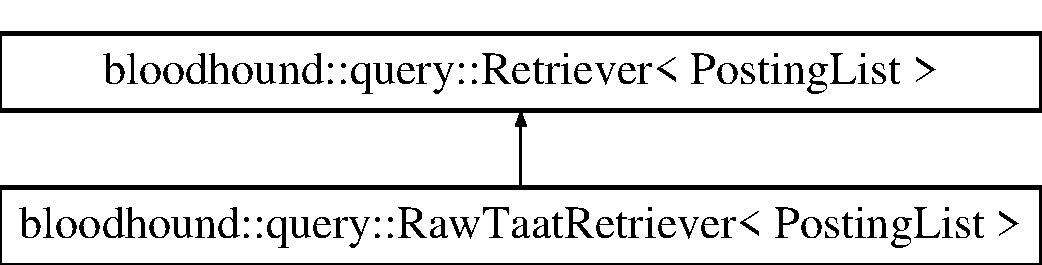
\includegraphics[height=2.000000cm]{classbloodhound_1_1query_1_1RawTaatRetriever}
\end{center}
\end{figure}
\subsection*{Public Member Functions}
\begin{DoxyCompactItemize}
\item 
\hyperlink{classbloodhound_1_1query_1_1RawTaatRetriever_a859b1cd2092da229964e2795c4445d72}{Raw\+Taat\+Retriever} (std\+::size\+\_\+t collection\+\_\+size)
\item 
void \hyperlink{classbloodhound_1_1query_1_1RawTaatRetriever_a70007a6dd5213e9c28266e38b424ba20}{traverse} (const std\+::vector$<$ \hyperlink{classbloodhound_1_1PostingList}{Posting\+List} $>$ \&lists\+\_\+for\+\_\+terms, const std\+::vector$<$ \hyperlink{structbloodhound_1_1Score}{Score} $>$ \&term\+\_\+weights)
\begin{DoxyCompactList}\small\item\em Traverses the postings and accumulates the scores. \end{DoxyCompactList}\item 
virtual std\+::vector$<$ \hyperlink{structbloodhound_1_1query_1_1Result}{Result} $>$ \hyperlink{classbloodhound_1_1query_1_1RawTaatRetriever_aafaaf842fdaef297a255e28766af2c0d}{retrieve} (const std\+::vector$<$ \hyperlink{classbloodhound_1_1PostingList}{Posting\+List} $>$ \&lists\+\_\+for\+\_\+terms, const std\+::vector$<$ \hyperlink{structbloodhound_1_1Score}{Score} $>$ \&term\+\_\+weights, std\+::size\+\_\+t k)
\begin{DoxyCompactList}\small\item\em Retrieves top-\/k results for the given posting lists and term weights. \end{DoxyCompactList}\end{DoxyCompactItemize}


\subsection{Constructor \& Destructor Documentation}
\mbox{\Hypertarget{classbloodhound_1_1query_1_1RawTaatRetriever_a859b1cd2092da229964e2795c4445d72}\label{classbloodhound_1_1query_1_1RawTaatRetriever_a859b1cd2092da229964e2795c4445d72}} 
\index{bloodhound\+::query\+::\+Raw\+Taat\+Retriever@{bloodhound\+::query\+::\+Raw\+Taat\+Retriever}!Raw\+Taat\+Retriever@{Raw\+Taat\+Retriever}}
\index{Raw\+Taat\+Retriever@{Raw\+Taat\+Retriever}!bloodhound\+::query\+::\+Raw\+Taat\+Retriever@{bloodhound\+::query\+::\+Raw\+Taat\+Retriever}}
\subsubsection{\texorpdfstring{Raw\+Taat\+Retriever()}{RawTaatRetriever()}}
{\footnotesize\ttfamily template$<$typename Posting\+List $>$ \\
\hyperlink{classbloodhound_1_1query_1_1RawTaatRetriever}{bloodhound\+::query\+::\+Raw\+Taat\+Retriever}$<$ \hyperlink{classbloodhound_1_1PostingList}{Posting\+List} $>$\+::\hyperlink{classbloodhound_1_1query_1_1RawTaatRetriever}{Raw\+Taat\+Retriever} (\begin{DoxyParamCaption}\item[{std\+::size\+\_\+t}]{collection\+\_\+size }\end{DoxyParamCaption})\hspace{0.3cm}{\ttfamily [inline]}}



\subsection{Member Function Documentation}
\mbox{\Hypertarget{classbloodhound_1_1query_1_1RawTaatRetriever_aafaaf842fdaef297a255e28766af2c0d}\label{classbloodhound_1_1query_1_1RawTaatRetriever_aafaaf842fdaef297a255e28766af2c0d}} 
\index{bloodhound\+::query\+::\+Raw\+Taat\+Retriever@{bloodhound\+::query\+::\+Raw\+Taat\+Retriever}!retrieve@{retrieve}}
\index{retrieve@{retrieve}!bloodhound\+::query\+::\+Raw\+Taat\+Retriever@{bloodhound\+::query\+::\+Raw\+Taat\+Retriever}}
\subsubsection{\texorpdfstring{retrieve()}{retrieve()}}
{\footnotesize\ttfamily template$<$typename Posting\+List $>$ \\
virtual std\+::vector$<$\hyperlink{structbloodhound_1_1query_1_1Result}{Result}$>$ \hyperlink{classbloodhound_1_1query_1_1RawTaatRetriever}{bloodhound\+::query\+::\+Raw\+Taat\+Retriever}$<$ \hyperlink{classbloodhound_1_1PostingList}{Posting\+List} $>$\+::retrieve (\begin{DoxyParamCaption}\item[{const std\+::vector$<$ \hyperlink{classbloodhound_1_1PostingList}{Posting\+List} $>$ \&}]{term\+\_\+postings,  }\item[{const std\+::vector$<$ \hyperlink{structbloodhound_1_1Score}{Score} $>$ \&}]{term\+\_\+weights,  }\item[{std\+::size\+\_\+t}]{k }\end{DoxyParamCaption})\hspace{0.3cm}{\ttfamily [inline]}, {\ttfamily [virtual]}}



Retrieves top-\/k results for the given posting lists and term weights. 



Implements \hyperlink{classbloodhound_1_1query_1_1Retriever_ae3c6a4628c5580e620c213b3dcd47c2b}{bloodhound\+::query\+::\+Retriever$<$ Posting\+List $>$}.

\mbox{\Hypertarget{classbloodhound_1_1query_1_1RawTaatRetriever_a70007a6dd5213e9c28266e38b424ba20}\label{classbloodhound_1_1query_1_1RawTaatRetriever_a70007a6dd5213e9c28266e38b424ba20}} 
\index{bloodhound\+::query\+::\+Raw\+Taat\+Retriever@{bloodhound\+::query\+::\+Raw\+Taat\+Retriever}!traverse@{traverse}}
\index{traverse@{traverse}!bloodhound\+::query\+::\+Raw\+Taat\+Retriever@{bloodhound\+::query\+::\+Raw\+Taat\+Retriever}}
\subsubsection{\texorpdfstring{traverse()}{traverse()}}
{\footnotesize\ttfamily template$<$typename Posting\+List $>$ \\
void \hyperlink{classbloodhound_1_1query_1_1RawTaatRetriever}{bloodhound\+::query\+::\+Raw\+Taat\+Retriever}$<$ \hyperlink{classbloodhound_1_1PostingList}{Posting\+List} $>$\+::traverse (\begin{DoxyParamCaption}\item[{const std\+::vector$<$ \hyperlink{classbloodhound_1_1PostingList}{Posting\+List} $>$ \&}]{lists\+\_\+for\+\_\+terms,  }\item[{const std\+::vector$<$ \hyperlink{structbloodhound_1_1Score}{Score} $>$ \&}]{term\+\_\+weights }\end{DoxyParamCaption})\hspace{0.3cm}{\ttfamily [inline]}}



Traverses the postings and accumulates the scores. 



The documentation for this class was generated from the following file\+:\begin{DoxyCompactItemize}
\item 
include/\hyperlink{retrievers_8hpp}{retrievers.\+hpp}\end{DoxyCompactItemize}

\hypertarget{structbloodhound_1_1RelativeOffset}{}\section{bloodhound\+:\+:Relative\+Offset Struct Reference}
\label{structbloodhound_1_1RelativeOffset}\index{bloodhound\+::\+Relative\+Offset@{bloodhound\+::\+Relative\+Offset}}


{\ttfamily \#include $<$index.\+hpp$>$}

Inheritance diagram for bloodhound\+:\+:Relative\+Offset\+:\begin{figure}[H]
\begin{center}
\leavevmode
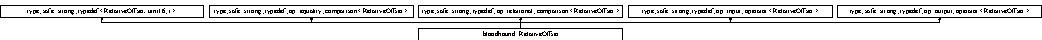
\includegraphics[height=0.534606cm]{structbloodhound_1_1RelativeOffset}
\end{center}
\end{figure}
\subsection*{Friends}
\begin{DoxyCompactItemize}
\item 
const char $\ast$ \hyperlink{structbloodhound_1_1RelativeOffset_a878bac48143c1d3b2597273daca07f25}{operator+} (const char $\ast$ptr, \hyperlink{structbloodhound_1_1RelativeOffset}{Relative\+Offset} offset)
\item 
char $\ast$ \hyperlink{structbloodhound_1_1RelativeOffset_aef76589aeb04376cde5936475652ceda}{operator+} (char $\ast$ptr, \hyperlink{structbloodhound_1_1RelativeOffset}{Relative\+Offset} offset)
\end{DoxyCompactItemize}


\subsection{Friends And Related Function Documentation}
\mbox{\Hypertarget{structbloodhound_1_1RelativeOffset_a878bac48143c1d3b2597273daca07f25}\label{structbloodhound_1_1RelativeOffset_a878bac48143c1d3b2597273daca07f25}} 
\index{bloodhound\+::\+Relative\+Offset@{bloodhound\+::\+Relative\+Offset}!operator+@{operator+}}
\index{operator+@{operator+}!bloodhound\+::\+Relative\+Offset@{bloodhound\+::\+Relative\+Offset}}
\subsubsection{\texorpdfstring{operator+}{operator+}\hspace{0.1cm}{\footnotesize\ttfamily [1/2]}}
{\footnotesize\ttfamily const char$\ast$ operator+ (\begin{DoxyParamCaption}\item[{const char $\ast$}]{ptr,  }\item[{\hyperlink{structbloodhound_1_1RelativeOffset}{Relative\+Offset}}]{offset }\end{DoxyParamCaption})\hspace{0.3cm}{\ttfamily [friend]}}

\mbox{\Hypertarget{structbloodhound_1_1RelativeOffset_aef76589aeb04376cde5936475652ceda}\label{structbloodhound_1_1RelativeOffset_aef76589aeb04376cde5936475652ceda}} 
\index{bloodhound\+::\+Relative\+Offset@{bloodhound\+::\+Relative\+Offset}!operator+@{operator+}}
\index{operator+@{operator+}!bloodhound\+::\+Relative\+Offset@{bloodhound\+::\+Relative\+Offset}}
\subsubsection{\texorpdfstring{operator+}{operator+}\hspace{0.1cm}{\footnotesize\ttfamily [2/2]}}
{\footnotesize\ttfamily char$\ast$ operator+ (\begin{DoxyParamCaption}\item[{char $\ast$}]{ptr,  }\item[{\hyperlink{structbloodhound_1_1RelativeOffset}{Relative\+Offset}}]{offset }\end{DoxyParamCaption})\hspace{0.3cm}{\ttfamily [friend]}}



The documentation for this struct was generated from the following file\+:\begin{DoxyCompactItemize}
\item 
include/\hyperlink{index_8hpp}{index.\+hpp}\end{DoxyCompactItemize}

\hypertarget{structbloodhound_1_1query_1_1Result}{}\section{bloodhound\+:\+:query\+:\+:Result Struct Reference}
\label{structbloodhound_1_1query_1_1Result}\index{bloodhound\+::query\+::\+Result@{bloodhound\+::query\+::\+Result}}


{\ttfamily \#include $<$query.\+hpp$>$}

\subsection*{Public Member Functions}
\begin{DoxyCompactItemize}
\item 
\mbox{\hyperlink{structbloodhound_1_1query_1_1Result_a6a9aaa804dbe3929b653b614e18408e1}{Result}} ()=default
\item 
\mbox{\hyperlink{structbloodhound_1_1query_1_1Result_ac4c15cb4d9e60b3e7bf37bd813215f55}{Result}} (\mbox{\hyperlink{structbloodhound_1_1Doc}{Doc}} d, \mbox{\hyperlink{structbloodhound_1_1Score}{Score}} s)
\item 
bool \mbox{\hyperlink{structbloodhound_1_1query_1_1Result_af7fa537e271f9f8b213e207331d5e647}{operator==}} (const \mbox{\hyperlink{structbloodhound_1_1query_1_1Result}{Result}} \&rhs) const
\item 
bool \mbox{\hyperlink{structbloodhound_1_1query_1_1Result_aafd7ab327a6ae26df25272b1ad1ec4c0}{operator$<$}} (const \mbox{\hyperlink{structbloodhound_1_1query_1_1Result}{Result}} \&rhs) const
\item 
bool \mbox{\hyperlink{structbloodhound_1_1query_1_1Result_a5af24f990ab7687d25e25b1f66dfb8a3}{operator$>$=}} (const \mbox{\hyperlink{structbloodhound_1_1query_1_1Result}{Result}} \&rhs) const
\item 
bool \mbox{\hyperlink{structbloodhound_1_1query_1_1Result_af04b71da89ecfa88ee4836dd82fdc058}{operator$>$}} (const \mbox{\hyperlink{structbloodhound_1_1query_1_1Result}{Result}} \&rhs) const
\end{DoxyCompactItemize}
\subsection*{Public Attributes}
\begin{DoxyCompactItemize}
\item 
\mbox{\hyperlink{structbloodhound_1_1Doc}{Doc}} \mbox{\hyperlink{structbloodhound_1_1query_1_1Result_a5f6acbb120aaf435333e410c0595962a}{doc}}
\item 
\mbox{\hyperlink{structbloodhound_1_1Score}{Score}} \mbox{\hyperlink{structbloodhound_1_1query_1_1Result_af9f240e486460b5130eff110b0f3c7a3}{score}}
\end{DoxyCompactItemize}


\subsection{Detailed Description}
Search result, consisting of the document\textquotesingle{}s ID and score. Any external ID or title is excluded, you must use a title mapping to retrieve it. 

\subsection{Constructor \& Destructor Documentation}
\mbox{\Hypertarget{structbloodhound_1_1query_1_1Result_a6a9aaa804dbe3929b653b614e18408e1}\label{structbloodhound_1_1query_1_1Result_a6a9aaa804dbe3929b653b614e18408e1}} 
\index{bloodhound\+::query\+::\+Result@{bloodhound\+::query\+::\+Result}!Result@{Result}}
\index{Result@{Result}!bloodhound\+::query\+::\+Result@{bloodhound\+::query\+::\+Result}}
\subsubsection{\texorpdfstring{Result()}{Result()}\hspace{0.1cm}{\footnotesize\ttfamily [1/2]}}
{\footnotesize\ttfamily bloodhound\+::query\+::\+Result\+::\+Result (\begin{DoxyParamCaption}{ }\end{DoxyParamCaption})\hspace{0.3cm}{\ttfamily [default]}}

\mbox{\Hypertarget{structbloodhound_1_1query_1_1Result_ac4c15cb4d9e60b3e7bf37bd813215f55}\label{structbloodhound_1_1query_1_1Result_ac4c15cb4d9e60b3e7bf37bd813215f55}} 
\index{bloodhound\+::query\+::\+Result@{bloodhound\+::query\+::\+Result}!Result@{Result}}
\index{Result@{Result}!bloodhound\+::query\+::\+Result@{bloodhound\+::query\+::\+Result}}
\subsubsection{\texorpdfstring{Result()}{Result()}\hspace{0.1cm}{\footnotesize\ttfamily [2/2]}}
{\footnotesize\ttfamily bloodhound\+::query\+::\+Result\+::\+Result (\begin{DoxyParamCaption}\item[{\mbox{\hyperlink{structbloodhound_1_1Doc}{Doc}}}]{d,  }\item[{\mbox{\hyperlink{structbloodhound_1_1Score}{Score}}}]{s }\end{DoxyParamCaption})\hspace{0.3cm}{\ttfamily [inline]}}



\subsection{Member Function Documentation}
\mbox{\Hypertarget{structbloodhound_1_1query_1_1Result_aafd7ab327a6ae26df25272b1ad1ec4c0}\label{structbloodhound_1_1query_1_1Result_aafd7ab327a6ae26df25272b1ad1ec4c0}} 
\index{bloodhound\+::query\+::\+Result@{bloodhound\+::query\+::\+Result}!operator$<$@{operator$<$}}
\index{operator$<$@{operator$<$}!bloodhound\+::query\+::\+Result@{bloodhound\+::query\+::\+Result}}
\subsubsection{\texorpdfstring{operator$<$()}{operator<()}}
{\footnotesize\ttfamily bool bloodhound\+::query\+::\+Result\+::operator$<$ (\begin{DoxyParamCaption}\item[{const \mbox{\hyperlink{structbloodhound_1_1query_1_1Result}{Result}} \&}]{rhs }\end{DoxyParamCaption}) const\hspace{0.3cm}{\ttfamily [inline]}}

\mbox{\Hypertarget{structbloodhound_1_1query_1_1Result_af7fa537e271f9f8b213e207331d5e647}\label{structbloodhound_1_1query_1_1Result_af7fa537e271f9f8b213e207331d5e647}} 
\index{bloodhound\+::query\+::\+Result@{bloodhound\+::query\+::\+Result}!operator==@{operator==}}
\index{operator==@{operator==}!bloodhound\+::query\+::\+Result@{bloodhound\+::query\+::\+Result}}
\subsubsection{\texorpdfstring{operator==()}{operator==()}}
{\footnotesize\ttfamily bool bloodhound\+::query\+::\+Result\+::operator== (\begin{DoxyParamCaption}\item[{const \mbox{\hyperlink{structbloodhound_1_1query_1_1Result}{Result}} \&}]{rhs }\end{DoxyParamCaption}) const\hspace{0.3cm}{\ttfamily [inline]}}

\mbox{\Hypertarget{structbloodhound_1_1query_1_1Result_af04b71da89ecfa88ee4836dd82fdc058}\label{structbloodhound_1_1query_1_1Result_af04b71da89ecfa88ee4836dd82fdc058}} 
\index{bloodhound\+::query\+::\+Result@{bloodhound\+::query\+::\+Result}!operator$>$@{operator$>$}}
\index{operator$>$@{operator$>$}!bloodhound\+::query\+::\+Result@{bloodhound\+::query\+::\+Result}}
\subsubsection{\texorpdfstring{operator$>$()}{operator>()}}
{\footnotesize\ttfamily bool bloodhound\+::query\+::\+Result\+::operator$>$ (\begin{DoxyParamCaption}\item[{const \mbox{\hyperlink{structbloodhound_1_1query_1_1Result}{Result}} \&}]{rhs }\end{DoxyParamCaption}) const\hspace{0.3cm}{\ttfamily [inline]}}

\mbox{\Hypertarget{structbloodhound_1_1query_1_1Result_a5af24f990ab7687d25e25b1f66dfb8a3}\label{structbloodhound_1_1query_1_1Result_a5af24f990ab7687d25e25b1f66dfb8a3}} 
\index{bloodhound\+::query\+::\+Result@{bloodhound\+::query\+::\+Result}!operator$>$=@{operator$>$=}}
\index{operator$>$=@{operator$>$=}!bloodhound\+::query\+::\+Result@{bloodhound\+::query\+::\+Result}}
\subsubsection{\texorpdfstring{operator$>$=()}{operator>=()}}
{\footnotesize\ttfamily bool bloodhound\+::query\+::\+Result\+::operator$>$= (\begin{DoxyParamCaption}\item[{const \mbox{\hyperlink{structbloodhound_1_1query_1_1Result}{Result}} \&}]{rhs }\end{DoxyParamCaption}) const\hspace{0.3cm}{\ttfamily [inline]}}



\subsection{Member Data Documentation}
\mbox{\Hypertarget{structbloodhound_1_1query_1_1Result_a5f6acbb120aaf435333e410c0595962a}\label{structbloodhound_1_1query_1_1Result_a5f6acbb120aaf435333e410c0595962a}} 
\index{bloodhound\+::query\+::\+Result@{bloodhound\+::query\+::\+Result}!doc@{doc}}
\index{doc@{doc}!bloodhound\+::query\+::\+Result@{bloodhound\+::query\+::\+Result}}
\subsubsection{\texorpdfstring{doc}{doc}}
{\footnotesize\ttfamily \mbox{\hyperlink{structbloodhound_1_1Doc}{Doc}} bloodhound\+::query\+::\+Result\+::doc}

\mbox{\Hypertarget{structbloodhound_1_1query_1_1Result_af9f240e486460b5130eff110b0f3c7a3}\label{structbloodhound_1_1query_1_1Result_af9f240e486460b5130eff110b0f3c7a3}} 
\index{bloodhound\+::query\+::\+Result@{bloodhound\+::query\+::\+Result}!score@{score}}
\index{score@{score}!bloodhound\+::query\+::\+Result@{bloodhound\+::query\+::\+Result}}
\subsubsection{\texorpdfstring{score}{score}}
{\footnotesize\ttfamily \mbox{\hyperlink{structbloodhound_1_1Score}{Score}} bloodhound\+::query\+::\+Result\+::score}



The documentation for this struct was generated from the following file\+:\begin{DoxyCompactItemize}
\item 
include/\mbox{\hyperlink{query_8hpp}{query.\+hpp}}\end{DoxyCompactItemize}

\hypertarget{classbloodhound_1_1query_1_1Retriever}{}\section{bloodhound\+:\+:query\+:\+:Retriever$<$ Posting\+List $>$ Class Template Reference}
\label{classbloodhound_1_1query_1_1Retriever}\index{bloodhound\+::query\+::\+Retriever$<$ Posting\+List $>$@{bloodhound\+::query\+::\+Retriever$<$ Posting\+List $>$}}


A base abstract super-\/class of all document retrievers.  




{\ttfamily \#include $<$query.\+hpp$>$}

Inheritance diagram for bloodhound\+:\+:query\+:\+:Retriever$<$ Posting\+List $>$\+:\begin{figure}[H]
\begin{center}
\leavevmode
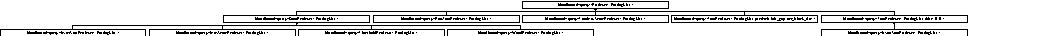
\includegraphics[height=0.484848cm]{classbloodhound_1_1query_1_1Retriever}
\end{center}
\end{figure}
\subsection*{Public Member Functions}
\begin{DoxyCompactItemize}
\item 
virtual std\+::vector$<$ \mbox{\hyperlink{structbloodhound_1_1query_1_1Result}{Result}} $>$ \mbox{\hyperlink{classbloodhound_1_1query_1_1Retriever_ae3c6a4628c5580e620c213b3dcd47c2b}{retrieve}} (const std\+::vector$<$ \mbox{\hyperlink{classbloodhound_1_1PostingList}{Posting\+List}} $>$ \&term\+\_\+postings, const std\+::vector$<$ \mbox{\hyperlink{structbloodhound_1_1Score}{Score}} $>$ \&term\+\_\+weights, std\+::size\+\_\+t k)=0
\begin{DoxyCompactList}\small\item\em Retrieves top-\/k results for the given posting lists and term weights. \end{DoxyCompactList}\item 
virtual nlohmann\+::json \mbox{\hyperlink{classbloodhound_1_1query_1_1Retriever_a58da32a5139b980ba874f8b5e6bb89ec}{stats}} ()
\end{DoxyCompactItemize}


\subsection{Detailed Description}
\subsubsection*{template$<$typename Posting\+List$>$\newline
class bloodhound\+::query\+::\+Retriever$<$ Posting\+List $>$}

A base abstract super-\/class of all document retrievers. 

\subsection{Member Function Documentation}
\mbox{\Hypertarget{classbloodhound_1_1query_1_1Retriever_ae3c6a4628c5580e620c213b3dcd47c2b}\label{classbloodhound_1_1query_1_1Retriever_ae3c6a4628c5580e620c213b3dcd47c2b}} 
\index{bloodhound\+::query\+::\+Retriever@{bloodhound\+::query\+::\+Retriever}!retrieve@{retrieve}}
\index{retrieve@{retrieve}!bloodhound\+::query\+::\+Retriever@{bloodhound\+::query\+::\+Retriever}}
\subsubsection{\texorpdfstring{retrieve()}{retrieve()}}
{\footnotesize\ttfamily template$<$typename Posting\+List $>$ \\
virtual std\+::vector$<$\mbox{\hyperlink{structbloodhound_1_1query_1_1Result}{Result}}$>$ \mbox{\hyperlink{classbloodhound_1_1query_1_1Retriever}{bloodhound\+::query\+::\+Retriever}}$<$ \mbox{\hyperlink{classbloodhound_1_1PostingList}{Posting\+List}} $>$\+::retrieve (\begin{DoxyParamCaption}\item[{const std\+::vector$<$ \mbox{\hyperlink{classbloodhound_1_1PostingList}{Posting\+List}} $>$ \&}]{term\+\_\+postings,  }\item[{const std\+::vector$<$ \mbox{\hyperlink{structbloodhound_1_1Score}{Score}} $>$ \&}]{term\+\_\+weights,  }\item[{std\+::size\+\_\+t}]{k }\end{DoxyParamCaption})\hspace{0.3cm}{\ttfamily [pure virtual]}}



Retrieves top-\/k results for the given posting lists and term weights. 



Implemented in \mbox{\hyperlink{classbloodhound_1_1query_1_1TaatMaxScoreRetriever_af4d96478395b58527969526c3068e7b9}{bloodhound\+::query\+::\+Taat\+Max\+Score\+Retriever$<$ Posting\+List $>$}}, \mbox{\hyperlink{classbloodhound_1_1query_1_1RawTaatRetriever_aafaaf842fdaef297a255e28766af2c0d}{bloodhound\+::query\+::\+Raw\+Taat\+Retriever$<$ Posting\+List $>$}}, \mbox{\hyperlink{classbloodhound_1_1query_1_1TaatRetriever_a58284f19458689021a083c07ea627485}{bloodhound\+::query\+::\+Taat\+Retriever$<$ Posting\+List, prefetch, init\+\_\+gap, acc\+\_\+block\+\_\+size $>$}}, \mbox{\hyperlink{classbloodhound_1_1query_1_1TaatRetriever_a58284f19458689021a083c07ea627485}{bloodhound\+::query\+::\+Taat\+Retriever$<$ Posting\+List, false, 0, 0 $>$}}, \mbox{\hyperlink{classbloodhound_1_1query_1_1WandRetriever_a5f3068bc363c16c5b7255a925ea5af8c}{bloodhound\+::query\+::\+Wand\+Retriever$<$ Posting\+List $>$}}, \mbox{\hyperlink{classbloodhound_1_1query_1_1ThresholdRetriever_a06750450e1246e755ebad2d5dac6e8a8}{bloodhound\+::query\+::\+Threshold\+Retriever$<$ Posting\+List $>$}}, \mbox{\hyperlink{classbloodhound_1_1query_1_1DaatRetriever_ab80b4867fc263827dc2fdbe0965a2e8c}{bloodhound\+::query\+::\+Daat\+Retriever$<$ Posting\+List $>$}}, and \mbox{\hyperlink{classbloodhound_1_1query_1_1ExactSaatRetriever_aced2763cc2a4c12838fef4a20759049e}{bloodhound\+::query\+::\+Exact\+Saat\+Retriever$<$ Posting\+List $>$}}.

\mbox{\Hypertarget{classbloodhound_1_1query_1_1Retriever_a58da32a5139b980ba874f8b5e6bb89ec}\label{classbloodhound_1_1query_1_1Retriever_a58da32a5139b980ba874f8b5e6bb89ec}} 
\index{bloodhound\+::query\+::\+Retriever@{bloodhound\+::query\+::\+Retriever}!stats@{stats}}
\index{stats@{stats}!bloodhound\+::query\+::\+Retriever@{bloodhound\+::query\+::\+Retriever}}
\subsubsection{\texorpdfstring{stats()}{stats()}}
{\footnotesize\ttfamily template$<$typename Posting\+List $>$ \\
virtual nlohmann\+::json \mbox{\hyperlink{classbloodhound_1_1query_1_1Retriever}{bloodhound\+::query\+::\+Retriever}}$<$ \mbox{\hyperlink{classbloodhound_1_1PostingList}{Posting\+List}} $>$\+::stats (\begin{DoxyParamCaption}{ }\end{DoxyParamCaption})\hspace{0.3cm}{\ttfamily [inline]}, {\ttfamily [virtual]}}



Reimplemented in \mbox{\hyperlink{classbloodhound_1_1query_1_1WandRetriever_a1e593c2cddb2ca4f2415c59ca26e6a36}{bloodhound\+::query\+::\+Wand\+Retriever$<$ Posting\+List $>$}}, \mbox{\hyperlink{classbloodhound_1_1query_1_1ThresholdRetriever_aa21e5b44d70bfdf058e5f9c5a1abc008}{bloodhound\+::query\+::\+Threshold\+Retriever$<$ Posting\+List $>$}}, and \mbox{\hyperlink{classbloodhound_1_1query_1_1ExactSaatRetriever_a716838f463f124964e76f48bc37d32cc}{bloodhound\+::query\+::\+Exact\+Saat\+Retriever$<$ Posting\+List $>$}}.



The documentation for this class was generated from the following file\+:\begin{DoxyCompactItemize}
\item 
include/\mbox{\hyperlink{query_8hpp}{query.\+hpp}}\end{DoxyCompactItemize}

\hypertarget{structbloodhound_1_1Score}{}\section{bloodhound\+:\+:Score Struct Reference}
\label{structbloodhound_1_1Score}\index{bloodhound\+::\+Score@{bloodhound\+::\+Score}}


{\ttfamily \#include $<$index.\+hpp$>$}

Inheritance diagram for bloodhound\+:\+:Score\+:\begin{figure}[H]
\begin{center}
\leavevmode
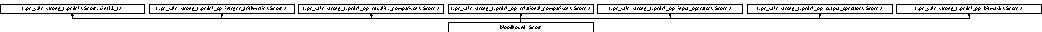
\includegraphics[height=0.427808cm]{structbloodhound_1_1Score}
\end{center}
\end{figure}


The documentation for this struct was generated from the following file\+:\begin{DoxyCompactItemize}
\item 
include/\mbox{\hyperlink{index_8hpp}{index.\+hpp}}\end{DoxyCompactItemize}

\hypertarget{structbloodhound_1_1score__greater}{}\section{bloodhound\+:\+:score\+\_\+greater$<$ Posting $>$ Struct Template Reference}
\label{structbloodhound_1_1score__greater}\index{bloodhound\+::score\+\_\+greater$<$ Posting $>$@{bloodhound\+::score\+\_\+greater$<$ Posting $>$}}


{\ttfamily \#include $<$index.\+hpp$>$}

\subsection*{Public Member Functions}
\begin{DoxyCompactItemize}
\item 
bool \hyperlink{structbloodhound_1_1score__greater_a56a430279ebf5d6b2526335fe3b2d668}{operator()} (const \hyperlink{structbloodhound_1_1Posting}{Posting} \&lhs, const \hyperlink{structbloodhound_1_1Posting}{Posting} \&rhs)
\end{DoxyCompactItemize}


\subsection{Member Function Documentation}
\mbox{\Hypertarget{structbloodhound_1_1score__greater_a56a430279ebf5d6b2526335fe3b2d668}\label{structbloodhound_1_1score__greater_a56a430279ebf5d6b2526335fe3b2d668}} 
\index{bloodhound\+::score\+\_\+greater@{bloodhound\+::score\+\_\+greater}!operator()@{operator()}}
\index{operator()@{operator()}!bloodhound\+::score\+\_\+greater@{bloodhound\+::score\+\_\+greater}}
\subsubsection{\texorpdfstring{operator()()}{operator()()}}
{\footnotesize\ttfamily template$<$class Posting $>$ \\
bool \hyperlink{structbloodhound_1_1score__greater}{bloodhound\+::score\+\_\+greater}$<$ \hyperlink{structbloodhound_1_1Posting}{Posting} $>$\+::operator() (\begin{DoxyParamCaption}\item[{const \hyperlink{structbloodhound_1_1Posting}{Posting} \&}]{lhs,  }\item[{const \hyperlink{structbloodhound_1_1Posting}{Posting} \&}]{rhs }\end{DoxyParamCaption})\hspace{0.3cm}{\ttfamily [inline]}}



The documentation for this struct was generated from the following file\+:\begin{DoxyCompactItemize}
\item 
include/\hyperlink{index_8hpp}{index.\+hpp}\end{DoxyCompactItemize}

\hypertarget{classirkit_1_1SimpleAccumulator}{}\section{irkit\+:\+:Simple\+Accumulator Class Reference}
\label{classirkit_1_1SimpleAccumulator}\index{irkit\+::\+Simple\+Accumulator@{irkit\+::\+Simple\+Accumulator}}


{\ttfamily \#include $<$taat.\+hpp$>$}

\subsection*{Public Member Functions}
\begin{DoxyCompactItemize}
\item 
{\footnotesize template$<$typename Doc , typename Score , typename Accumulator\+Array $>$ }\\void \hyperlink{classirkit_1_1SimpleAccumulator_af747d80dbebe394e3ebe920afeeac810}{accumulate\+\_\+posting} (Doc doc, Score score\+\_\+delta, Accumulator\+Array \&acc)
\begin{DoxyCompactList}\small\item\em Accumulates the posting that is being processed. \end{DoxyCompactList}\end{DoxyCompactItemize}


\subsection{Member Function Documentation}
\mbox{\Hypertarget{classirkit_1_1SimpleAccumulator_af747d80dbebe394e3ebe920afeeac810}\label{classirkit_1_1SimpleAccumulator_af747d80dbebe394e3ebe920afeeac810}} 
\index{irkit\+::\+Simple\+Accumulator@{irkit\+::\+Simple\+Accumulator}!accumulate\+\_\+posting@{accumulate\+\_\+posting}}
\index{accumulate\+\_\+posting@{accumulate\+\_\+posting}!irkit\+::\+Simple\+Accumulator@{irkit\+::\+Simple\+Accumulator}}
\subsubsection{\texorpdfstring{accumulate\+\_\+posting()}{accumulate\_posting()}}
{\footnotesize\ttfamily template$<$typename Doc , typename Score , typename Accumulator\+Array $>$ \\
void irkit\+::\+Simple\+Accumulator\+::accumulate\+\_\+posting (\begin{DoxyParamCaption}\item[{Doc}]{doc,  }\item[{Score}]{score\+\_\+delta,  }\item[{Accumulator\+Array \&}]{acc }\end{DoxyParamCaption})\hspace{0.3cm}{\ttfamily [inline]}}



Accumulates the posting that is being processed. 



The documentation for this class was generated from the following file\+:\begin{DoxyCompactItemize}
\item 
include/\hyperlink{taat_8hpp}{taat.\+hpp}\end{DoxyCompactItemize}

\hypertarget{classbloodhound_1_1query_1_1TaatMaxScoreRetriever}{}\section{bloodhound\+:\+:query\+:\+:Taat\+Max\+Score\+Retriever$<$ Posting\+List $>$ Class Template Reference}
\label{classbloodhound_1_1query_1_1TaatMaxScoreRetriever}\index{bloodhound\+::query\+::\+Taat\+Max\+Score\+Retriever$<$ Posting\+List $>$@{bloodhound\+::query\+::\+Taat\+Max\+Score\+Retriever$<$ Posting\+List $>$}}


{\ttfamily \#include $<$retrievers.\+hpp$>$}

Inheritance diagram for bloodhound\+:\+:query\+:\+:Taat\+Max\+Score\+Retriever$<$ Posting\+List $>$\+:\begin{figure}[H]
\begin{center}
\leavevmode
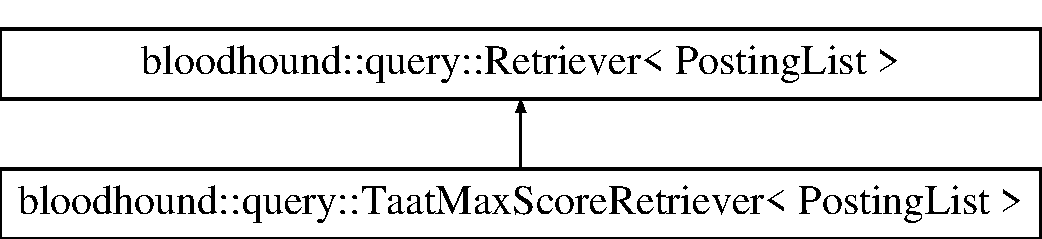
\includegraphics[height=2.000000cm]{classbloodhound_1_1query_1_1TaatMaxScoreRetriever}
\end{center}
\end{figure}
\subsection*{Public Member Functions}
\begin{DoxyCompactItemize}
\item 
\mbox{\hyperlink{classbloodhound_1_1query_1_1TaatMaxScoreRetriever_a8f452aa87a82194bf337e4ce6a06c1f4}{Taat\+Max\+Score\+Retriever}} (std\+::size\+\_\+t collection\+\_\+size)
\item 
std\+::vector$<$ std\+::size\+\_\+t $>$ \mbox{\hyperlink{classbloodhound_1_1query_1_1TaatMaxScoreRetriever_a4c5253dee6541cf173f4f2e16803c702}{sorted\+\_\+by\+\_\+length}} (const std\+::vector$<$ \mbox{\hyperlink{classbloodhound_1_1PostingList}{Posting\+List}} $>$ \&lists\+\_\+for\+\_\+terms)
\item 
virtual std\+::vector$<$ \mbox{\hyperlink{structbloodhound_1_1query_1_1Result}{Result}} $>$ \mbox{\hyperlink{classbloodhound_1_1query_1_1TaatMaxScoreRetriever_af4d96478395b58527969526c3068e7b9}{retrieve}} (const std\+::vector$<$ \mbox{\hyperlink{classbloodhound_1_1PostingList}{Posting\+List}} $>$ \&lists\+\_\+for\+\_\+terms, const std\+::vector$<$ \mbox{\hyperlink{structbloodhound_1_1Score}{Score}} $>$ \&term\+\_\+weights, std\+::size\+\_\+t k)
\begin{DoxyCompactList}\small\item\em Retrieves top-\/k results for the given posting lists and term weights. \end{DoxyCompactList}\end{DoxyCompactItemize}


\subsection{Constructor \& Destructor Documentation}
\mbox{\Hypertarget{classbloodhound_1_1query_1_1TaatMaxScoreRetriever_a8f452aa87a82194bf337e4ce6a06c1f4}\label{classbloodhound_1_1query_1_1TaatMaxScoreRetriever_a8f452aa87a82194bf337e4ce6a06c1f4}} 
\index{bloodhound\+::query\+::\+Taat\+Max\+Score\+Retriever@{bloodhound\+::query\+::\+Taat\+Max\+Score\+Retriever}!Taat\+Max\+Score\+Retriever@{Taat\+Max\+Score\+Retriever}}
\index{Taat\+Max\+Score\+Retriever@{Taat\+Max\+Score\+Retriever}!bloodhound\+::query\+::\+Taat\+Max\+Score\+Retriever@{bloodhound\+::query\+::\+Taat\+Max\+Score\+Retriever}}
\subsubsection{\texorpdfstring{Taat\+Max\+Score\+Retriever()}{TaatMaxScoreRetriever()}}
{\footnotesize\ttfamily template$<$typename Posting\+List $>$ \\
\mbox{\hyperlink{classbloodhound_1_1query_1_1TaatMaxScoreRetriever}{bloodhound\+::query\+::\+Taat\+Max\+Score\+Retriever}}$<$ \mbox{\hyperlink{classbloodhound_1_1PostingList}{Posting\+List}} $>$\+::\mbox{\hyperlink{classbloodhound_1_1query_1_1TaatMaxScoreRetriever}{Taat\+Max\+Score\+Retriever}} (\begin{DoxyParamCaption}\item[{std\+::size\+\_\+t}]{collection\+\_\+size }\end{DoxyParamCaption})\hspace{0.3cm}{\ttfamily [inline]}}



\subsection{Member Function Documentation}
\mbox{\Hypertarget{classbloodhound_1_1query_1_1TaatMaxScoreRetriever_af4d96478395b58527969526c3068e7b9}\label{classbloodhound_1_1query_1_1TaatMaxScoreRetriever_af4d96478395b58527969526c3068e7b9}} 
\index{bloodhound\+::query\+::\+Taat\+Max\+Score\+Retriever@{bloodhound\+::query\+::\+Taat\+Max\+Score\+Retriever}!retrieve@{retrieve}}
\index{retrieve@{retrieve}!bloodhound\+::query\+::\+Taat\+Max\+Score\+Retriever@{bloodhound\+::query\+::\+Taat\+Max\+Score\+Retriever}}
\subsubsection{\texorpdfstring{retrieve()}{retrieve()}}
{\footnotesize\ttfamily template$<$typename Posting\+List $>$ \\
virtual std\+::vector$<$\mbox{\hyperlink{structbloodhound_1_1query_1_1Result}{Result}}$>$ \mbox{\hyperlink{classbloodhound_1_1query_1_1TaatMaxScoreRetriever}{bloodhound\+::query\+::\+Taat\+Max\+Score\+Retriever}}$<$ \mbox{\hyperlink{classbloodhound_1_1PostingList}{Posting\+List}} $>$\+::retrieve (\begin{DoxyParamCaption}\item[{const std\+::vector$<$ \mbox{\hyperlink{classbloodhound_1_1PostingList}{Posting\+List}} $>$ \&}]{term\+\_\+postings,  }\item[{const std\+::vector$<$ \mbox{\hyperlink{structbloodhound_1_1Score}{Score}} $>$ \&}]{term\+\_\+weights,  }\item[{std\+::size\+\_\+t}]{k }\end{DoxyParamCaption})\hspace{0.3cm}{\ttfamily [inline]}, {\ttfamily [virtual]}}



Retrieves top-\/k results for the given posting lists and term weights. 



Implements \mbox{\hyperlink{classbloodhound_1_1query_1_1Retriever_ae3c6a4628c5580e620c213b3dcd47c2b}{bloodhound\+::query\+::\+Retriever$<$ Posting\+List $>$}}.

\mbox{\Hypertarget{classbloodhound_1_1query_1_1TaatMaxScoreRetriever_a4c5253dee6541cf173f4f2e16803c702}\label{classbloodhound_1_1query_1_1TaatMaxScoreRetriever_a4c5253dee6541cf173f4f2e16803c702}} 
\index{bloodhound\+::query\+::\+Taat\+Max\+Score\+Retriever@{bloodhound\+::query\+::\+Taat\+Max\+Score\+Retriever}!sorted\+\_\+by\+\_\+length@{sorted\+\_\+by\+\_\+length}}
\index{sorted\+\_\+by\+\_\+length@{sorted\+\_\+by\+\_\+length}!bloodhound\+::query\+::\+Taat\+Max\+Score\+Retriever@{bloodhound\+::query\+::\+Taat\+Max\+Score\+Retriever}}
\subsubsection{\texorpdfstring{sorted\+\_\+by\+\_\+length()}{sorted\_by\_length()}}
{\footnotesize\ttfamily template$<$typename Posting\+List $>$ \\
std\+::vector$<$std\+::size\+\_\+t$>$ \mbox{\hyperlink{classbloodhound_1_1query_1_1TaatMaxScoreRetriever}{bloodhound\+::query\+::\+Taat\+Max\+Score\+Retriever}}$<$ \mbox{\hyperlink{classbloodhound_1_1PostingList}{Posting\+List}} $>$\+::sorted\+\_\+by\+\_\+length (\begin{DoxyParamCaption}\item[{const std\+::vector$<$ \mbox{\hyperlink{classbloodhound_1_1PostingList}{Posting\+List}} $>$ \&}]{lists\+\_\+for\+\_\+terms }\end{DoxyParamCaption})\hspace{0.3cm}{\ttfamily [inline]}}



The documentation for this class was generated from the following file\+:\begin{DoxyCompactItemize}
\item 
include/\mbox{\hyperlink{retrievers_8hpp}{retrievers.\+hpp}}\end{DoxyCompactItemize}

\hypertarget{classbloodhound_1_1query_1_1TaatRetriever}{}\section{bloodhound\+:\+:query\+:\+:Taat\+Retriever$<$ Posting\+List, prefetch, init\+\_\+gap, acc\+\_\+block\+\_\+size $>$ Class Template Reference}
\label{classbloodhound_1_1query_1_1TaatRetriever}\index{bloodhound\+::query\+::\+Taat\+Retriever$<$ Posting\+List, prefetch, init\+\_\+gap, acc\+\_\+block\+\_\+size $>$@{bloodhound\+::query\+::\+Taat\+Retriever$<$ Posting\+List, prefetch, init\+\_\+gap, acc\+\_\+block\+\_\+size $>$}}


{\ttfamily \#include $<$retrievers.\+hpp$>$}

Inheritance diagram for bloodhound\+:\+:query\+:\+:Taat\+Retriever$<$ Posting\+List, prefetch, init\+\_\+gap, acc\+\_\+block\+\_\+size $>$\+:\begin{figure}[H]
\begin{center}
\leavevmode
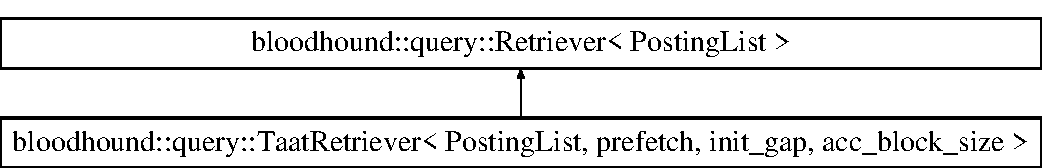
\includegraphics[height=2.000000cm]{classbloodhound_1_1query_1_1TaatRetriever}
\end{center}
\end{figure}
\subsection*{Public Member Functions}
\begin{DoxyCompactItemize}
\item 
\hyperlink{classbloodhound_1_1query_1_1TaatRetriever_af443da08f4200fb84a3481d47bc4ac35}{Taat\+Retriever} (std\+::size\+\_\+t collection\+\_\+size)
\begin{DoxyCompactList}\small\item\em Constructs a \hyperlink{classbloodhound_1_1query_1_1TaatRetriever}{Taat\+Retriever} with an accumulator array of collection\+\_\+size. \end{DoxyCompactList}\item 
void \hyperlink{classbloodhound_1_1query_1_1TaatRetriever_a34def8d627b446d7459792ab9c50dcab}{accumulate\+\_\+posting} (\hyperlink{structbloodhound_1_1Doc}{Doc} doc, \hyperlink{structbloodhound_1_1Score}{Score} score\+\_\+delta, std\+::vector$<$ \hyperlink{structbloodhound_1_1Score}{Score} $>$ \&acc)
\begin{DoxyCompactList}\small\item\em Accumulates the posting that is being processed. \end{DoxyCompactList}\item 
void \hyperlink{classbloodhound_1_1query_1_1TaatRetriever_a1b476e4ada85862cb79a92b6424d2aa2}{traverse} (const std\+::vector$<$ \hyperlink{classbloodhound_1_1PostingList}{Posting\+List} $>$ \&lists\+\_\+for\+\_\+terms, const std\+::vector$<$ \hyperlink{structbloodhound_1_1Score}{Score} $>$ \&term\+\_\+weights)
\begin{DoxyCompactList}\small\item\em Traverses a single posting lists and accumulates its scores. \end{DoxyCompactList}\item 
\hyperlink{structbloodhound_1_1Score}{Score} \hyperlink{classbloodhound_1_1query_1_1TaatRetriever_ae1c8d9643ca85ba7dba32325538e30b5}{score\+\_\+of} (\hyperlink{structbloodhound_1_1Doc}{Doc} doc) const
\begin{DoxyCompactList}\small\item\em Returns the accumulated score of doc. \end{DoxyCompactList}\item 
std\+::vector$<$ \hyperlink{structbloodhound_1_1query_1_1Result}{Result} $>$ \hyperlink{classbloodhound_1_1query_1_1TaatRetriever_a7f631f87075249c768873d15a59956c5}{aggregate\+\_\+top} (std\+::size\+\_\+t k)
\item 
void \hyperlink{classbloodhound_1_1query_1_1TaatRetriever_a6fedf448e3d9394ecaa787bf60a9cb84}{clear\+\_\+accumulator\+\_\+array} ()
\begin{DoxyCompactList}\small\item\em Fill the accumulator array with zeroes. \end{DoxyCompactList}\item 
void \hyperlink{classbloodhound_1_1query_1_1TaatRetriever_a00a64711e5d865ba4c53e3accdb61d3f}{clear\+\_\+blocks} ()
\begin{DoxyCompactList}\small\item\em Set all block maximum scores with zeroes. \end{DoxyCompactList}\item 
void \hyperlink{classbloodhound_1_1query_1_1TaatRetriever_ad6739ab7025c6de9e65945cff25c55b4}{next\+\_\+query} ()
\item 
virtual std\+::vector$<$ \hyperlink{structbloodhound_1_1query_1_1Result}{Result} $>$ \hyperlink{classbloodhound_1_1query_1_1TaatRetriever_a58284f19458689021a083c07ea627485}{retrieve} (const std\+::vector$<$ \hyperlink{classbloodhound_1_1PostingList}{Posting\+List} $>$ \&lists\+\_\+for\+\_\+terms, const std\+::vector$<$ \hyperlink{structbloodhound_1_1Score}{Score} $>$ \&term\+\_\+weights, std\+::size\+\_\+t k)
\begin{DoxyCompactList}\small\item\em Retrieves top-\/k results for the given posting lists and term weights. \end{DoxyCompactList}\end{DoxyCompactItemize}
\subsection*{Protected Attributes}
\begin{DoxyCompactItemize}
\item 
\hyperlink{namespacebloodhound_1_1query_aa67214af106292b2483995adea986b08}{Query\+Id} \hyperlink{classbloodhound_1_1query_1_1TaatRetriever_aa9a1b8ca0cb570bcffe6b6c68e8c2e20}{query\+\_\+id}
\item 
\hyperlink{structbloodhound_1_1Score}{Score} \hyperlink{classbloodhound_1_1query_1_1TaatRetriever_aa27d16b326df60affe26e005f9abb4f6}{qidx\+\_\+shifted}
\item 
\hyperlink{structbloodhound_1_1Score}{Score} \hyperlink{classbloodhound_1_1query_1_1TaatRetriever_ac38b873ceff34b55bb8ac82800946825}{score\+\_\+mask}
\item 
unsigned int \hyperlink{classbloodhound_1_1query_1_1TaatRetriever_aa2b4875de4f02a856e64560bf002296f}{bits\+\_\+to\+\_\+shift}
\item 
std\+::vector$<$ \hyperlink{structbloodhound_1_1Score}{Score} $>$ \hyperlink{classbloodhound_1_1query_1_1TaatRetriever_a604c7ab279ced03ccc1866d55c844b11}{accumulator\+\_\+array}
\begin{DoxyCompactList}\small\item\em The array of accumulated values for each document. \end{DoxyCompactList}\item 
std\+::vector$<$ \hyperlink{structbloodhound_1_1Score}{Score} $>$ \hyperlink{classbloodhound_1_1query_1_1TaatRetriever_ac870574844dc3be6c40cf1236e1ff6cc}{block\+\_\+max\+\_\+scores}
\item 
std\+::size\+\_\+t \hyperlink{classbloodhound_1_1query_1_1TaatRetriever_a87786d9af7993da498d60304eab245cf}{nblocks}
\end{DoxyCompactItemize}


\subsection{Detailed Description}
\subsubsection*{template$<$typename Posting\+List, bool prefetch = false, unsigned short init\+\_\+gap = 0, unsigned int acc\+\_\+block\+\_\+size = 0$>$\newline
class bloodhound\+::query\+::\+Taat\+Retriever$<$ Posting\+List, prefetch, init\+\_\+gap, acc\+\_\+block\+\_\+size $>$}

Term-\/at-\/a-\/time document retriever.

\hyperlink{classbloodhound_1_1PostingList}{Posting\+List} requires\+:
\begin{DoxyItemize}
\item doc\+\_\+begin() and doc\+\_\+end()\+: document start and end iterator, respectively;
\item score\+\_\+begin() and score\+\_\+end()\+: score start and end iterator, respectively;
\item length()\+: posting list length; 
\end{DoxyItemize}

\subsection{Constructor \& Destructor Documentation}
\mbox{\Hypertarget{classbloodhound_1_1query_1_1TaatRetriever_af443da08f4200fb84a3481d47bc4ac35}\label{classbloodhound_1_1query_1_1TaatRetriever_af443da08f4200fb84a3481d47bc4ac35}} 
\index{bloodhound\+::query\+::\+Taat\+Retriever@{bloodhound\+::query\+::\+Taat\+Retriever}!Taat\+Retriever@{Taat\+Retriever}}
\index{Taat\+Retriever@{Taat\+Retriever}!bloodhound\+::query\+::\+Taat\+Retriever@{bloodhound\+::query\+::\+Taat\+Retriever}}
\subsubsection{\texorpdfstring{Taat\+Retriever()}{TaatRetriever()}}
{\footnotesize\ttfamily template$<$typename Posting\+List, bool prefetch = false, unsigned short init\+\_\+gap = 0, unsigned int acc\+\_\+block\+\_\+size = 0$>$ \\
\hyperlink{classbloodhound_1_1query_1_1TaatRetriever}{bloodhound\+::query\+::\+Taat\+Retriever}$<$ \hyperlink{classbloodhound_1_1PostingList}{Posting\+List}, prefetch, init\+\_\+gap, acc\+\_\+block\+\_\+size $>$\+::\hyperlink{classbloodhound_1_1query_1_1TaatRetriever}{Taat\+Retriever} (\begin{DoxyParamCaption}\item[{std\+::size\+\_\+t}]{collection\+\_\+size }\end{DoxyParamCaption})\hspace{0.3cm}{\ttfamily [inline]}}



Constructs a \hyperlink{classbloodhound_1_1query_1_1TaatRetriever}{Taat\+Retriever} with an accumulator array of collection\+\_\+size. 



\subsection{Member Function Documentation}
\mbox{\Hypertarget{classbloodhound_1_1query_1_1TaatRetriever_a34def8d627b446d7459792ab9c50dcab}\label{classbloodhound_1_1query_1_1TaatRetriever_a34def8d627b446d7459792ab9c50dcab}} 
\index{bloodhound\+::query\+::\+Taat\+Retriever@{bloodhound\+::query\+::\+Taat\+Retriever}!accumulate\+\_\+posting@{accumulate\+\_\+posting}}
\index{accumulate\+\_\+posting@{accumulate\+\_\+posting}!bloodhound\+::query\+::\+Taat\+Retriever@{bloodhound\+::query\+::\+Taat\+Retriever}}
\subsubsection{\texorpdfstring{accumulate\+\_\+posting()}{accumulate\_posting()}}
{\footnotesize\ttfamily template$<$typename Posting\+List, bool prefetch = false, unsigned short init\+\_\+gap = 0, unsigned int acc\+\_\+block\+\_\+size = 0$>$ \\
void \hyperlink{classbloodhound_1_1query_1_1TaatRetriever}{bloodhound\+::query\+::\+Taat\+Retriever}$<$ \hyperlink{classbloodhound_1_1PostingList}{Posting\+List}, prefetch, init\+\_\+gap, acc\+\_\+block\+\_\+size $>$\+::accumulate\+\_\+posting (\begin{DoxyParamCaption}\item[{\hyperlink{structbloodhound_1_1Doc}{Doc}}]{doc,  }\item[{\hyperlink{structbloodhound_1_1Score}{Score}}]{score\+\_\+delta,  }\item[{std\+::vector$<$ \hyperlink{structbloodhound_1_1Score}{Score} $>$ \&}]{acc }\end{DoxyParamCaption})\hspace{0.3cm}{\ttfamily [inline]}}



Accumulates the posting that is being processed. 

\mbox{\Hypertarget{classbloodhound_1_1query_1_1TaatRetriever_a7f631f87075249c768873d15a59956c5}\label{classbloodhound_1_1query_1_1TaatRetriever_a7f631f87075249c768873d15a59956c5}} 
\index{bloodhound\+::query\+::\+Taat\+Retriever@{bloodhound\+::query\+::\+Taat\+Retriever}!aggregate\+\_\+top@{aggregate\+\_\+top}}
\index{aggregate\+\_\+top@{aggregate\+\_\+top}!bloodhound\+::query\+::\+Taat\+Retriever@{bloodhound\+::query\+::\+Taat\+Retriever}}
\subsubsection{\texorpdfstring{aggregate\+\_\+top()}{aggregate\_top()}}
{\footnotesize\ttfamily template$<$typename Posting\+List, bool prefetch = false, unsigned short init\+\_\+gap = 0, unsigned int acc\+\_\+block\+\_\+size = 0$>$ \\
std\+::vector$<$\hyperlink{structbloodhound_1_1query_1_1Result}{Result}$>$ \hyperlink{classbloodhound_1_1query_1_1TaatRetriever}{bloodhound\+::query\+::\+Taat\+Retriever}$<$ \hyperlink{classbloodhound_1_1PostingList}{Posting\+List}, prefetch, init\+\_\+gap, acc\+\_\+block\+\_\+size $>$\+::aggregate\+\_\+top (\begin{DoxyParamCaption}\item[{std\+::size\+\_\+t}]{k }\end{DoxyParamCaption})\hspace{0.3cm}{\ttfamily [inline]}}

Returns the top-\/k highest ranked documents.

It may return fewer documents if fewer of them contain any term. \mbox{\Hypertarget{classbloodhound_1_1query_1_1TaatRetriever_a6fedf448e3d9394ecaa787bf60a9cb84}\label{classbloodhound_1_1query_1_1TaatRetriever_a6fedf448e3d9394ecaa787bf60a9cb84}} 
\index{bloodhound\+::query\+::\+Taat\+Retriever@{bloodhound\+::query\+::\+Taat\+Retriever}!clear\+\_\+accumulator\+\_\+array@{clear\+\_\+accumulator\+\_\+array}}
\index{clear\+\_\+accumulator\+\_\+array@{clear\+\_\+accumulator\+\_\+array}!bloodhound\+::query\+::\+Taat\+Retriever@{bloodhound\+::query\+::\+Taat\+Retriever}}
\subsubsection{\texorpdfstring{clear\+\_\+accumulator\+\_\+array()}{clear\_accumulator\_array()}}
{\footnotesize\ttfamily template$<$typename Posting\+List, bool prefetch = false, unsigned short init\+\_\+gap = 0, unsigned int acc\+\_\+block\+\_\+size = 0$>$ \\
void \hyperlink{classbloodhound_1_1query_1_1TaatRetriever}{bloodhound\+::query\+::\+Taat\+Retriever}$<$ \hyperlink{classbloodhound_1_1PostingList}{Posting\+List}, prefetch, init\+\_\+gap, acc\+\_\+block\+\_\+size $>$\+::clear\+\_\+accumulator\+\_\+array (\begin{DoxyParamCaption}{ }\end{DoxyParamCaption})\hspace{0.3cm}{\ttfamily [inline]}}



Fill the accumulator array with zeroes. 

\mbox{\Hypertarget{classbloodhound_1_1query_1_1TaatRetriever_a00a64711e5d865ba4c53e3accdb61d3f}\label{classbloodhound_1_1query_1_1TaatRetriever_a00a64711e5d865ba4c53e3accdb61d3f}} 
\index{bloodhound\+::query\+::\+Taat\+Retriever@{bloodhound\+::query\+::\+Taat\+Retriever}!clear\+\_\+blocks@{clear\+\_\+blocks}}
\index{clear\+\_\+blocks@{clear\+\_\+blocks}!bloodhound\+::query\+::\+Taat\+Retriever@{bloodhound\+::query\+::\+Taat\+Retriever}}
\subsubsection{\texorpdfstring{clear\+\_\+blocks()}{clear\_blocks()}}
{\footnotesize\ttfamily template$<$typename Posting\+List, bool prefetch = false, unsigned short init\+\_\+gap = 0, unsigned int acc\+\_\+block\+\_\+size = 0$>$ \\
void \hyperlink{classbloodhound_1_1query_1_1TaatRetriever}{bloodhound\+::query\+::\+Taat\+Retriever}$<$ \hyperlink{classbloodhound_1_1PostingList}{Posting\+List}, prefetch, init\+\_\+gap, acc\+\_\+block\+\_\+size $>$\+::clear\+\_\+blocks (\begin{DoxyParamCaption}{ }\end{DoxyParamCaption})\hspace{0.3cm}{\ttfamily [inline]}}



Set all block maximum scores with zeroes. 

\mbox{\Hypertarget{classbloodhound_1_1query_1_1TaatRetriever_ad6739ab7025c6de9e65945cff25c55b4}\label{classbloodhound_1_1query_1_1TaatRetriever_ad6739ab7025c6de9e65945cff25c55b4}} 
\index{bloodhound\+::query\+::\+Taat\+Retriever@{bloodhound\+::query\+::\+Taat\+Retriever}!next\+\_\+query@{next\+\_\+query}}
\index{next\+\_\+query@{next\+\_\+query}!bloodhound\+::query\+::\+Taat\+Retriever@{bloodhound\+::query\+::\+Taat\+Retriever}}
\subsubsection{\texorpdfstring{next\+\_\+query()}{next\_query()}}
{\footnotesize\ttfamily template$<$typename Posting\+List, bool prefetch = false, unsigned short init\+\_\+gap = 0, unsigned int acc\+\_\+block\+\_\+size = 0$>$ \\
void \hyperlink{classbloodhound_1_1query_1_1TaatRetriever}{bloodhound\+::query\+::\+Taat\+Retriever}$<$ \hyperlink{classbloodhound_1_1PostingList}{Posting\+List}, prefetch, init\+\_\+gap, acc\+\_\+block\+\_\+size $>$\+::next\+\_\+query (\begin{DoxyParamCaption}{ }\end{DoxyParamCaption})\hspace{0.3cm}{\ttfamily [inline]}}

Proceed to the next query.

Clears the accumulators if necessary and keeps track of the query I\+Ds. \mbox{\Hypertarget{classbloodhound_1_1query_1_1TaatRetriever_a58284f19458689021a083c07ea627485}\label{classbloodhound_1_1query_1_1TaatRetriever_a58284f19458689021a083c07ea627485}} 
\index{bloodhound\+::query\+::\+Taat\+Retriever@{bloodhound\+::query\+::\+Taat\+Retriever}!retrieve@{retrieve}}
\index{retrieve@{retrieve}!bloodhound\+::query\+::\+Taat\+Retriever@{bloodhound\+::query\+::\+Taat\+Retriever}}
\subsubsection{\texorpdfstring{retrieve()}{retrieve()}}
{\footnotesize\ttfamily template$<$typename Posting\+List, bool prefetch = false, unsigned short init\+\_\+gap = 0, unsigned int acc\+\_\+block\+\_\+size = 0$>$ \\
virtual std\+::vector$<$\hyperlink{structbloodhound_1_1query_1_1Result}{Result}$>$ \hyperlink{classbloodhound_1_1query_1_1TaatRetriever}{bloodhound\+::query\+::\+Taat\+Retriever}$<$ \hyperlink{classbloodhound_1_1PostingList}{Posting\+List}, prefetch, init\+\_\+gap, acc\+\_\+block\+\_\+size $>$\+::retrieve (\begin{DoxyParamCaption}\item[{const std\+::vector$<$ \hyperlink{classbloodhound_1_1PostingList}{Posting\+List} $>$ \&}]{term\+\_\+postings,  }\item[{const std\+::vector$<$ \hyperlink{structbloodhound_1_1Score}{Score} $>$ \&}]{term\+\_\+weights,  }\item[{std\+::size\+\_\+t}]{k }\end{DoxyParamCaption})\hspace{0.3cm}{\ttfamily [inline]}, {\ttfamily [virtual]}}



Retrieves top-\/k results for the given posting lists and term weights. 



Implements \hyperlink{classbloodhound_1_1query_1_1Retriever_ae3c6a4628c5580e620c213b3dcd47c2b}{bloodhound\+::query\+::\+Retriever$<$ Posting\+List $>$}.



Reimplemented in \hyperlink{classbloodhound_1_1query_1_1ExactSaatRetriever_aced2763cc2a4c12838fef4a20759049e}{bloodhound\+::query\+::\+Exact\+Saat\+Retriever$<$ Posting\+List $>$}.

\mbox{\Hypertarget{classbloodhound_1_1query_1_1TaatRetriever_ae1c8d9643ca85ba7dba32325538e30b5}\label{classbloodhound_1_1query_1_1TaatRetriever_ae1c8d9643ca85ba7dba32325538e30b5}} 
\index{bloodhound\+::query\+::\+Taat\+Retriever@{bloodhound\+::query\+::\+Taat\+Retriever}!score\+\_\+of@{score\+\_\+of}}
\index{score\+\_\+of@{score\+\_\+of}!bloodhound\+::query\+::\+Taat\+Retriever@{bloodhound\+::query\+::\+Taat\+Retriever}}
\subsubsection{\texorpdfstring{score\+\_\+of()}{score\_of()}}
{\footnotesize\ttfamily template$<$typename Posting\+List, bool prefetch = false, unsigned short init\+\_\+gap = 0, unsigned int acc\+\_\+block\+\_\+size = 0$>$ \\
\hyperlink{structbloodhound_1_1Score}{Score} \hyperlink{classbloodhound_1_1query_1_1TaatRetriever}{bloodhound\+::query\+::\+Taat\+Retriever}$<$ \hyperlink{classbloodhound_1_1PostingList}{Posting\+List}, prefetch, init\+\_\+gap, acc\+\_\+block\+\_\+size $>$\+::score\+\_\+of (\begin{DoxyParamCaption}\item[{\hyperlink{structbloodhound_1_1Doc}{Doc}}]{doc }\end{DoxyParamCaption}) const\hspace{0.3cm}{\ttfamily [inline]}}



Returns the accumulated score of doc. 

\mbox{\Hypertarget{classbloodhound_1_1query_1_1TaatRetriever_a1b476e4ada85862cb79a92b6424d2aa2}\label{classbloodhound_1_1query_1_1TaatRetriever_a1b476e4ada85862cb79a92b6424d2aa2}} 
\index{bloodhound\+::query\+::\+Taat\+Retriever@{bloodhound\+::query\+::\+Taat\+Retriever}!traverse@{traverse}}
\index{traverse@{traverse}!bloodhound\+::query\+::\+Taat\+Retriever@{bloodhound\+::query\+::\+Taat\+Retriever}}
\subsubsection{\texorpdfstring{traverse()}{traverse()}}
{\footnotesize\ttfamily template$<$typename Posting\+List, bool prefetch = false, unsigned short init\+\_\+gap = 0, unsigned int acc\+\_\+block\+\_\+size = 0$>$ \\
void \hyperlink{classbloodhound_1_1query_1_1TaatRetriever}{bloodhound\+::query\+::\+Taat\+Retriever}$<$ \hyperlink{classbloodhound_1_1PostingList}{Posting\+List}, prefetch, init\+\_\+gap, acc\+\_\+block\+\_\+size $>$\+::traverse (\begin{DoxyParamCaption}\item[{const std\+::vector$<$ \hyperlink{classbloodhound_1_1PostingList}{Posting\+List} $>$ \&}]{lists\+\_\+for\+\_\+terms,  }\item[{const std\+::vector$<$ \hyperlink{structbloodhound_1_1Score}{Score} $>$ \&}]{term\+\_\+weights }\end{DoxyParamCaption})\hspace{0.3cm}{\ttfamily [inline]}}



Traverses a single posting lists and accumulates its scores. 

Traverses the postings and accumulates the scores. 

\subsection{Member Data Documentation}
\mbox{\Hypertarget{classbloodhound_1_1query_1_1TaatRetriever_a604c7ab279ced03ccc1866d55c844b11}\label{classbloodhound_1_1query_1_1TaatRetriever_a604c7ab279ced03ccc1866d55c844b11}} 
\index{bloodhound\+::query\+::\+Taat\+Retriever@{bloodhound\+::query\+::\+Taat\+Retriever}!accumulator\+\_\+array@{accumulator\+\_\+array}}
\index{accumulator\+\_\+array@{accumulator\+\_\+array}!bloodhound\+::query\+::\+Taat\+Retriever@{bloodhound\+::query\+::\+Taat\+Retriever}}
\subsubsection{\texorpdfstring{accumulator\+\_\+array}{accumulator\_array}}
{\footnotesize\ttfamily template$<$typename Posting\+List, bool prefetch = false, unsigned short init\+\_\+gap = 0, unsigned int acc\+\_\+block\+\_\+size = 0$>$ \\
std\+::vector$<$\hyperlink{structbloodhound_1_1Score}{Score}$>$ \hyperlink{classbloodhound_1_1query_1_1TaatRetriever}{bloodhound\+::query\+::\+Taat\+Retriever}$<$ \hyperlink{classbloodhound_1_1PostingList}{Posting\+List}, prefetch, init\+\_\+gap, acc\+\_\+block\+\_\+size $>$\+::accumulator\+\_\+array\hspace{0.3cm}{\ttfamily [protected]}}



The array of accumulated values for each document. 

\mbox{\Hypertarget{classbloodhound_1_1query_1_1TaatRetriever_aa2b4875de4f02a856e64560bf002296f}\label{classbloodhound_1_1query_1_1TaatRetriever_aa2b4875de4f02a856e64560bf002296f}} 
\index{bloodhound\+::query\+::\+Taat\+Retriever@{bloodhound\+::query\+::\+Taat\+Retriever}!bits\+\_\+to\+\_\+shift@{bits\+\_\+to\+\_\+shift}}
\index{bits\+\_\+to\+\_\+shift@{bits\+\_\+to\+\_\+shift}!bloodhound\+::query\+::\+Taat\+Retriever@{bloodhound\+::query\+::\+Taat\+Retriever}}
\subsubsection{\texorpdfstring{bits\+\_\+to\+\_\+shift}{bits\_to\_shift}}
{\footnotesize\ttfamily template$<$typename Posting\+List, bool prefetch = false, unsigned short init\+\_\+gap = 0, unsigned int acc\+\_\+block\+\_\+size = 0$>$ \\
unsigned int \hyperlink{classbloodhound_1_1query_1_1TaatRetriever}{bloodhound\+::query\+::\+Taat\+Retriever}$<$ \hyperlink{classbloodhound_1_1PostingList}{Posting\+List}, prefetch, init\+\_\+gap, acc\+\_\+block\+\_\+size $>$\+::bits\+\_\+to\+\_\+shift\hspace{0.3cm}{\ttfamily [protected]}}

How many bits are used for the score value. This is only used when init\+\_\+gap $>$ 1. \mbox{\Hypertarget{classbloodhound_1_1query_1_1TaatRetriever_ac870574844dc3be6c40cf1236e1ff6cc}\label{classbloodhound_1_1query_1_1TaatRetriever_ac870574844dc3be6c40cf1236e1ff6cc}} 
\index{bloodhound\+::query\+::\+Taat\+Retriever@{bloodhound\+::query\+::\+Taat\+Retriever}!block\+\_\+max\+\_\+scores@{block\+\_\+max\+\_\+scores}}
\index{block\+\_\+max\+\_\+scores@{block\+\_\+max\+\_\+scores}!bloodhound\+::query\+::\+Taat\+Retriever@{bloodhound\+::query\+::\+Taat\+Retriever}}
\subsubsection{\texorpdfstring{block\+\_\+max\+\_\+scores}{block\_max\_scores}}
{\footnotesize\ttfamily template$<$typename Posting\+List, bool prefetch = false, unsigned short init\+\_\+gap = 0, unsigned int acc\+\_\+block\+\_\+size = 0$>$ \\
std\+::vector$<$\hyperlink{structbloodhound_1_1Score}{Score}$>$ \hyperlink{classbloodhound_1_1query_1_1TaatRetriever}{bloodhound\+::query\+::\+Taat\+Retriever}$<$ \hyperlink{classbloodhound_1_1PostingList}{Posting\+List}, prefetch, init\+\_\+gap, acc\+\_\+block\+\_\+size $>$\+::block\+\_\+max\+\_\+scores\hspace{0.3cm}{\ttfamily [protected]}}

Maximum scores for each accumulator block. Only used when acc\+\_\+block\+\_\+size $>$ 0. \mbox{\Hypertarget{classbloodhound_1_1query_1_1TaatRetriever_a87786d9af7993da498d60304eab245cf}\label{classbloodhound_1_1query_1_1TaatRetriever_a87786d9af7993da498d60304eab245cf}} 
\index{bloodhound\+::query\+::\+Taat\+Retriever@{bloodhound\+::query\+::\+Taat\+Retriever}!nblocks@{nblocks}}
\index{nblocks@{nblocks}!bloodhound\+::query\+::\+Taat\+Retriever@{bloodhound\+::query\+::\+Taat\+Retriever}}
\subsubsection{\texorpdfstring{nblocks}{nblocks}}
{\footnotesize\ttfamily template$<$typename Posting\+List, bool prefetch = false, unsigned short init\+\_\+gap = 0, unsigned int acc\+\_\+block\+\_\+size = 0$>$ \\
std\+::size\+\_\+t \hyperlink{classbloodhound_1_1query_1_1TaatRetriever}{bloodhound\+::query\+::\+Taat\+Retriever}$<$ \hyperlink{classbloodhound_1_1PostingList}{Posting\+List}, prefetch, init\+\_\+gap, acc\+\_\+block\+\_\+size $>$\+::nblocks\hspace{0.3cm}{\ttfamily [protected]}}

The number of blocks, calculated based on acc\+\_\+block\+\_\+size and the number of documents in the index. Only used when acc\+\_\+block\+\_\+size $>$ 0. \mbox{\Hypertarget{classbloodhound_1_1query_1_1TaatRetriever_aa27d16b326df60affe26e005f9abb4f6}\label{classbloodhound_1_1query_1_1TaatRetriever_aa27d16b326df60affe26e005f9abb4f6}} 
\index{bloodhound\+::query\+::\+Taat\+Retriever@{bloodhound\+::query\+::\+Taat\+Retriever}!qidx\+\_\+shifted@{qidx\+\_\+shifted}}
\index{qidx\+\_\+shifted@{qidx\+\_\+shifted}!bloodhound\+::query\+::\+Taat\+Retriever@{bloodhound\+::query\+::\+Taat\+Retriever}}
\subsubsection{\texorpdfstring{qidx\+\_\+shifted}{qidx\_shifted}}
{\footnotesize\ttfamily template$<$typename Posting\+List, bool prefetch = false, unsigned short init\+\_\+gap = 0, unsigned int acc\+\_\+block\+\_\+size = 0$>$ \\
\hyperlink{structbloodhound_1_1Score}{Score} \hyperlink{classbloodhound_1_1query_1_1TaatRetriever}{bloodhound\+::query\+::\+Taat\+Retriever}$<$ \hyperlink{classbloodhound_1_1PostingList}{Posting\+List}, prefetch, init\+\_\+gap, acc\+\_\+block\+\_\+size $>$\+::qidx\+\_\+shifted\hspace{0.3cm}{\ttfamily [protected]}}

This is query\+\_\+id shifted to the far left for quick comparison of the accumulated values. This is only used when init\+\_\+gap $>$ 1. \mbox{\Hypertarget{classbloodhound_1_1query_1_1TaatRetriever_aa9a1b8ca0cb570bcffe6b6c68e8c2e20}\label{classbloodhound_1_1query_1_1TaatRetriever_aa9a1b8ca0cb570bcffe6b6c68e8c2e20}} 
\index{bloodhound\+::query\+::\+Taat\+Retriever@{bloodhound\+::query\+::\+Taat\+Retriever}!query\+\_\+id@{query\+\_\+id}}
\index{query\+\_\+id@{query\+\_\+id}!bloodhound\+::query\+::\+Taat\+Retriever@{bloodhound\+::query\+::\+Taat\+Retriever}}
\subsubsection{\texorpdfstring{query\+\_\+id}{query\_id}}
{\footnotesize\ttfamily template$<$typename Posting\+List, bool prefetch = false, unsigned short init\+\_\+gap = 0, unsigned int acc\+\_\+block\+\_\+size = 0$>$ \\
\hyperlink{namespacebloodhound_1_1query_aa67214af106292b2483995adea986b08}{Query\+Id} \hyperlink{classbloodhound_1_1query_1_1TaatRetriever}{bloodhound\+::query\+::\+Taat\+Retriever}$<$ \hyperlink{classbloodhound_1_1PostingList}{Posting\+List}, prefetch, init\+\_\+gap, acc\+\_\+block\+\_\+size $>$\+::query\+\_\+id\hspace{0.3cm}{\ttfamily [protected]}}

Keeps track of the accumulator clearing cycle. It is always in range \mbox{[}0, init\+\_\+gap), and is increased modulo init\+\_\+gap after each query. This is only used when init\+\_\+gap $>$ 1. \mbox{\Hypertarget{classbloodhound_1_1query_1_1TaatRetriever_ac38b873ceff34b55bb8ac82800946825}\label{classbloodhound_1_1query_1_1TaatRetriever_ac38b873ceff34b55bb8ac82800946825}} 
\index{bloodhound\+::query\+::\+Taat\+Retriever@{bloodhound\+::query\+::\+Taat\+Retriever}!score\+\_\+mask@{score\+\_\+mask}}
\index{score\+\_\+mask@{score\+\_\+mask}!bloodhound\+::query\+::\+Taat\+Retriever@{bloodhound\+::query\+::\+Taat\+Retriever}}
\subsubsection{\texorpdfstring{score\+\_\+mask}{score\_mask}}
{\footnotesize\ttfamily template$<$typename Posting\+List, bool prefetch = false, unsigned short init\+\_\+gap = 0, unsigned int acc\+\_\+block\+\_\+size = 0$>$ \\
\hyperlink{structbloodhound_1_1Score}{Score} \hyperlink{classbloodhound_1_1query_1_1TaatRetriever}{bloodhound\+::query\+::\+Taat\+Retriever}$<$ \hyperlink{classbloodhound_1_1PostingList}{Posting\+List}, prefetch, init\+\_\+gap, acc\+\_\+block\+\_\+size $>$\+::score\+\_\+mask\hspace{0.3cm}{\ttfamily [protected]}}

The score mask for fast computing of the accumulated values. This is only used when init\+\_\+gap $>$ 1. 

The documentation for this class was generated from the following file\+:\begin{DoxyCompactItemize}
\item 
include/\hyperlink{retrievers_8hpp}{retrievers.\+hpp}\end{DoxyCompactItemize}

\hypertarget{structbloodhound_1_1index_1_1format_1_1TermDetails}{}\section{bloodhound\+:\+:index\+:\+:format\+:\+:Term\+Details Struct Reference}
\label{structbloodhound_1_1index_1_1format_1_1TermDetails}\index{bloodhound\+::index\+::format\+::\+Term\+Details@{bloodhound\+::index\+::format\+::\+Term\+Details}}


{\ttfamily \#include $<$format.\+hpp$>$}

\subsection*{Public Attributes}
\begin{DoxyCompactItemize}
\item 
\mbox{\hyperlink{structbloodhound_1_1TermId}{Term\+Id}} \mbox{\hyperlink{structbloodhound_1_1index_1_1format_1_1TermDetails_a05890ba855986755276485d7753201ca}{term}}
\item 
\mbox{\hyperlink{structbloodhound_1_1Offset}{Offset}} \mbox{\hyperlink{structbloodhound_1_1index_1_1format_1_1TermDetails_a4361db3ce131c8c7beadf58bd651f1c3}{doc\+\_\+offset}}
\item 
\mbox{\hyperlink{structbloodhound_1_1Offset}{Offset}} \mbox{\hyperlink{structbloodhound_1_1index_1_1format_1_1TermDetails_aec8833fdbf2ae61ade0fe42ce8a7240c}{score\+\_\+offset}}
\end{DoxyCompactItemize}


\subsection{Member Data Documentation}
\mbox{\Hypertarget{structbloodhound_1_1index_1_1format_1_1TermDetails_a4361db3ce131c8c7beadf58bd651f1c3}\label{structbloodhound_1_1index_1_1format_1_1TermDetails_a4361db3ce131c8c7beadf58bd651f1c3}} 
\index{bloodhound\+::index\+::format\+::\+Term\+Details@{bloodhound\+::index\+::format\+::\+Term\+Details}!doc\+\_\+offset@{doc\+\_\+offset}}
\index{doc\+\_\+offset@{doc\+\_\+offset}!bloodhound\+::index\+::format\+::\+Term\+Details@{bloodhound\+::index\+::format\+::\+Term\+Details}}
\subsubsection{\texorpdfstring{doc\+\_\+offset}{doc\_offset}}
{\footnotesize\ttfamily \mbox{\hyperlink{structbloodhound_1_1Offset}{Offset}} bloodhound\+::index\+::format\+::\+Term\+Details\+::doc\+\_\+offset}

\mbox{\Hypertarget{structbloodhound_1_1index_1_1format_1_1TermDetails_aec8833fdbf2ae61ade0fe42ce8a7240c}\label{structbloodhound_1_1index_1_1format_1_1TermDetails_aec8833fdbf2ae61ade0fe42ce8a7240c}} 
\index{bloodhound\+::index\+::format\+::\+Term\+Details@{bloodhound\+::index\+::format\+::\+Term\+Details}!score\+\_\+offset@{score\+\_\+offset}}
\index{score\+\_\+offset@{score\+\_\+offset}!bloodhound\+::index\+::format\+::\+Term\+Details@{bloodhound\+::index\+::format\+::\+Term\+Details}}
\subsubsection{\texorpdfstring{score\+\_\+offset}{score\_offset}}
{\footnotesize\ttfamily \mbox{\hyperlink{structbloodhound_1_1Offset}{Offset}} bloodhound\+::index\+::format\+::\+Term\+Details\+::score\+\_\+offset}

\mbox{\Hypertarget{structbloodhound_1_1index_1_1format_1_1TermDetails_a05890ba855986755276485d7753201ca}\label{structbloodhound_1_1index_1_1format_1_1TermDetails_a05890ba855986755276485d7753201ca}} 
\index{bloodhound\+::index\+::format\+::\+Term\+Details@{bloodhound\+::index\+::format\+::\+Term\+Details}!term@{term}}
\index{term@{term}!bloodhound\+::index\+::format\+::\+Term\+Details@{bloodhound\+::index\+::format\+::\+Term\+Details}}
\subsubsection{\texorpdfstring{term}{term}}
{\footnotesize\ttfamily \mbox{\hyperlink{structbloodhound_1_1TermId}{Term\+Id}} bloodhound\+::index\+::format\+::\+Term\+Details\+::term}



The documentation for this struct was generated from the following file\+:\begin{DoxyCompactItemize}
\item 
include/index/\mbox{\hyperlink{format_8hpp}{format.\+hpp}}\end{DoxyCompactItemize}

\hypertarget{structbloodhound_1_1TermId}{}\section{bloodhound\+:\+:Term\+Id Struct Reference}
\label{structbloodhound_1_1TermId}\index{bloodhound\+::\+Term\+Id@{bloodhound\+::\+Term\+Id}}


{\ttfamily \#include $<$index.\+hpp$>$}

Inheritance diagram for bloodhound\+:\+:Term\+Id\+:\begin{figure}[H]
\begin{center}
\leavevmode
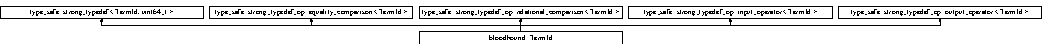
\includegraphics[height=0.592593cm]{structbloodhound_1_1TermId}
\end{center}
\end{figure}


The documentation for this struct was generated from the following file\+:\begin{DoxyCompactItemize}
\item 
include/\mbox{\hyperlink{index_8hpp}{index.\+hpp}}\end{DoxyCompactItemize}

\hypertarget{structbloodhound_1_1TermWeight}{}\section{bloodhound\+:\+:Term\+Weight Struct Reference}
\label{structbloodhound_1_1TermWeight}\index{bloodhound\+::\+Term\+Weight@{bloodhound\+::\+Term\+Weight}}


{\ttfamily \#include $<$index.\+hpp$>$}

\subsection*{Public Attributes}
\begin{DoxyCompactItemize}
\item 
\mbox{\hyperlink{structbloodhound_1_1TermId}{Term\+Id}} \mbox{\hyperlink{structbloodhound_1_1TermWeight_a8606421116b89015b89272bd5e2602a9}{term}}
\item 
\mbox{\hyperlink{structbloodhound_1_1Score}{Score}} \mbox{\hyperlink{structbloodhound_1_1TermWeight_a1abc2c53928fbaa8dcf617e72e1afced}{weight}}
\end{DoxyCompactItemize}


\subsection{Member Data Documentation}
\mbox{\Hypertarget{structbloodhound_1_1TermWeight_a8606421116b89015b89272bd5e2602a9}\label{structbloodhound_1_1TermWeight_a8606421116b89015b89272bd5e2602a9}} 
\index{bloodhound\+::\+Term\+Weight@{bloodhound\+::\+Term\+Weight}!term@{term}}
\index{term@{term}!bloodhound\+::\+Term\+Weight@{bloodhound\+::\+Term\+Weight}}
\subsubsection{\texorpdfstring{term}{term}}
{\footnotesize\ttfamily \mbox{\hyperlink{structbloodhound_1_1TermId}{Term\+Id}} bloodhound\+::\+Term\+Weight\+::term}

\mbox{\Hypertarget{structbloodhound_1_1TermWeight_a1abc2c53928fbaa8dcf617e72e1afced}\label{structbloodhound_1_1TermWeight_a1abc2c53928fbaa8dcf617e72e1afced}} 
\index{bloodhound\+::\+Term\+Weight@{bloodhound\+::\+Term\+Weight}!weight@{weight}}
\index{weight@{weight}!bloodhound\+::\+Term\+Weight@{bloodhound\+::\+Term\+Weight}}
\subsubsection{\texorpdfstring{weight}{weight}}
{\footnotesize\ttfamily \mbox{\hyperlink{structbloodhound_1_1Score}{Score}} bloodhound\+::\+Term\+Weight\+::weight}



The documentation for this struct was generated from the following file\+:\begin{DoxyCompactItemize}
\item 
include/\mbox{\hyperlink{index_8hpp}{index.\+hpp}}\end{DoxyCompactItemize}

\hypertarget{classbloodhound_1_1query_1_1ThresholdRetriever}{}\section{bloodhound\+:\+:query\+:\+:Threshold\+Retriever$<$ Posting\+List $>$ Class Template Reference}
\label{classbloodhound_1_1query_1_1ThresholdRetriever}\index{bloodhound\+::query\+::\+Threshold\+Retriever$<$ Posting\+List $>$@{bloodhound\+::query\+::\+Threshold\+Retriever$<$ Posting\+List $>$}}


{\ttfamily \#include $<$saat.\+hpp$>$}

Inheritance diagram for bloodhound\+:\+:query\+:\+:Threshold\+Retriever$<$ Posting\+List $>$\+:\begin{figure}[H]
\begin{center}
\leavevmode
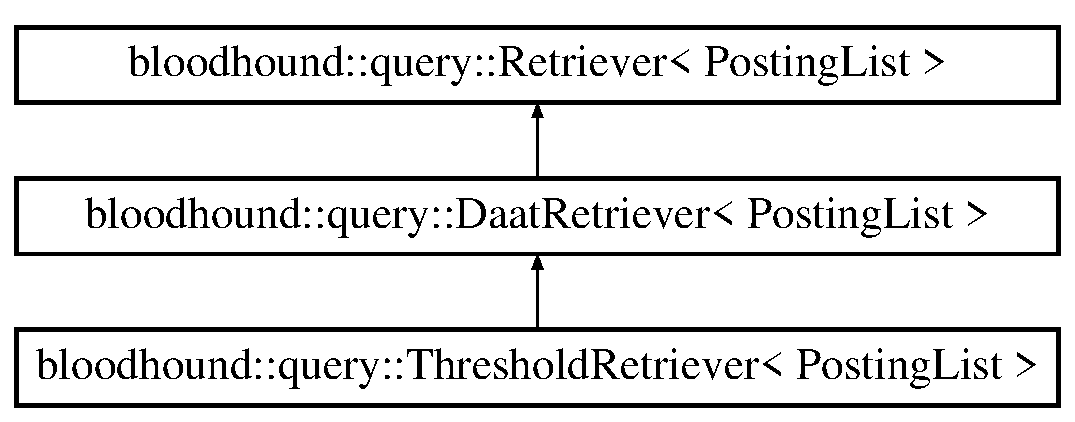
\includegraphics[height=3.000000cm]{classbloodhound_1_1query_1_1ThresholdRetriever}
\end{center}
\end{figure}
\subsection*{Public Member Functions}
\begin{DoxyCompactItemize}
\item 
\hyperlink{classbloodhound_1_1query_1_1ThresholdRetriever_a425d17d048e1fd3fd8157450c99df5bc}{Threshold\+Retriever} (std\+::size\+\_\+t collection\+\_\+size)
\item 
\hyperlink{structbloodhound_1_1Score}{Score} \hyperlink{classbloodhound_1_1query_1_1ThresholdRetriever_ac0a8731d270c477e04f24b89850a7d4a}{score\+\_\+with\+\_\+lookups} (\hyperlink{structbloodhound_1_1Doc}{Doc} doc, std\+::vector$<$ \hyperlink{structbloodhound_1_1Score}{Score} $>$ \&acc)
\item 
virtual std\+::vector$<$ \hyperlink{structbloodhound_1_1query_1_1Result}{Result} $>$ \hyperlink{classbloodhound_1_1query_1_1ThresholdRetriever_a06750450e1246e755ebad2d5dac6e8a8}{retrieve} (const std\+::vector$<$ \hyperlink{classbloodhound_1_1PostingList}{Posting\+List} $>$ \&term\+\_\+postings, const std\+::vector$<$ \hyperlink{structbloodhound_1_1Score}{Score} $>$ \&term\+\_\+weights, std\+::size\+\_\+t k)
\begin{DoxyCompactList}\small\item\em Retrieves top-\/k results for the given posting lists and term weights. \end{DoxyCompactList}\item 
virtual nlohmann\+::json \hyperlink{classbloodhound_1_1query_1_1ThresholdRetriever_aa21e5b44d70bfdf058e5f9c5a1abc008}{stats} ()
\end{DoxyCompactItemize}


\subsection{Detailed Description}
\subsubsection*{template$<$typename Posting\+List$>$\newline
class bloodhound\+::query\+::\+Threshold\+Retriever$<$ Posting\+List $>$}

Implementation of Fagin\textquotesingle{}s Threshold Algorithm.

Assumes that postings are sorted by their partial scores. 

\subsection{Constructor \& Destructor Documentation}
\mbox{\Hypertarget{classbloodhound_1_1query_1_1ThresholdRetriever_a425d17d048e1fd3fd8157450c99df5bc}\label{classbloodhound_1_1query_1_1ThresholdRetriever_a425d17d048e1fd3fd8157450c99df5bc}} 
\index{bloodhound\+::query\+::\+Threshold\+Retriever@{bloodhound\+::query\+::\+Threshold\+Retriever}!Threshold\+Retriever@{Threshold\+Retriever}}
\index{Threshold\+Retriever@{Threshold\+Retriever}!bloodhound\+::query\+::\+Threshold\+Retriever@{bloodhound\+::query\+::\+Threshold\+Retriever}}
\subsubsection{\texorpdfstring{Threshold\+Retriever()}{ThresholdRetriever()}}
{\footnotesize\ttfamily template$<$typename Posting\+List $>$ \\
\hyperlink{classbloodhound_1_1query_1_1ThresholdRetriever}{bloodhound\+::query\+::\+Threshold\+Retriever}$<$ \hyperlink{classbloodhound_1_1PostingList}{Posting\+List} $>$\+::\hyperlink{classbloodhound_1_1query_1_1ThresholdRetriever}{Threshold\+Retriever} (\begin{DoxyParamCaption}\item[{std\+::size\+\_\+t}]{collection\+\_\+size }\end{DoxyParamCaption})\hspace{0.3cm}{\ttfamily [inline]}}



\subsection{Member Function Documentation}
\mbox{\Hypertarget{classbloodhound_1_1query_1_1ThresholdRetriever_a06750450e1246e755ebad2d5dac6e8a8}\label{classbloodhound_1_1query_1_1ThresholdRetriever_a06750450e1246e755ebad2d5dac6e8a8}} 
\index{bloodhound\+::query\+::\+Threshold\+Retriever@{bloodhound\+::query\+::\+Threshold\+Retriever}!retrieve@{retrieve}}
\index{retrieve@{retrieve}!bloodhound\+::query\+::\+Threshold\+Retriever@{bloodhound\+::query\+::\+Threshold\+Retriever}}
\subsubsection{\texorpdfstring{retrieve()}{retrieve()}}
{\footnotesize\ttfamily template$<$typename Posting\+List $>$ \\
virtual std\+::vector$<$\hyperlink{structbloodhound_1_1query_1_1Result}{Result}$>$ \hyperlink{classbloodhound_1_1query_1_1ThresholdRetriever}{bloodhound\+::query\+::\+Threshold\+Retriever}$<$ \hyperlink{classbloodhound_1_1PostingList}{Posting\+List} $>$\+::retrieve (\begin{DoxyParamCaption}\item[{const std\+::vector$<$ \hyperlink{classbloodhound_1_1PostingList}{Posting\+List} $>$ \&}]{term\+\_\+postings,  }\item[{const std\+::vector$<$ \hyperlink{structbloodhound_1_1Score}{Score} $>$ \&}]{term\+\_\+weights,  }\item[{std\+::size\+\_\+t}]{k }\end{DoxyParamCaption})\hspace{0.3cm}{\ttfamily [inline]}, {\ttfamily [virtual]}}



Retrieves top-\/k results for the given posting lists and term weights. 



Reimplemented from \hyperlink{classbloodhound_1_1query_1_1DaatRetriever_ab80b4867fc263827dc2fdbe0965a2e8c}{bloodhound\+::query\+::\+Daat\+Retriever$<$ Posting\+List $>$}.

\mbox{\Hypertarget{classbloodhound_1_1query_1_1ThresholdRetriever_ac0a8731d270c477e04f24b89850a7d4a}\label{classbloodhound_1_1query_1_1ThresholdRetriever_ac0a8731d270c477e04f24b89850a7d4a}} 
\index{bloodhound\+::query\+::\+Threshold\+Retriever@{bloodhound\+::query\+::\+Threshold\+Retriever}!score\+\_\+with\+\_\+lookups@{score\+\_\+with\+\_\+lookups}}
\index{score\+\_\+with\+\_\+lookups@{score\+\_\+with\+\_\+lookups}!bloodhound\+::query\+::\+Threshold\+Retriever@{bloodhound\+::query\+::\+Threshold\+Retriever}}
\subsubsection{\texorpdfstring{score\+\_\+with\+\_\+lookups()}{score\_with\_lookups()}}
{\footnotesize\ttfamily template$<$typename Posting\+List $>$ \\
\hyperlink{structbloodhound_1_1Score}{Score} \hyperlink{classbloodhound_1_1query_1_1ThresholdRetriever}{bloodhound\+::query\+::\+Threshold\+Retriever}$<$ \hyperlink{classbloodhound_1_1PostingList}{Posting\+List} $>$\+::score\+\_\+with\+\_\+lookups (\begin{DoxyParamCaption}\item[{\hyperlink{structbloodhound_1_1Doc}{Doc}}]{doc,  }\item[{std\+::vector$<$ \hyperlink{structbloodhound_1_1Score}{Score} $>$ \&}]{acc }\end{DoxyParamCaption})\hspace{0.3cm}{\ttfamily [inline]}}

\mbox{\Hypertarget{classbloodhound_1_1query_1_1ThresholdRetriever_aa21e5b44d70bfdf058e5f9c5a1abc008}\label{classbloodhound_1_1query_1_1ThresholdRetriever_aa21e5b44d70bfdf058e5f9c5a1abc008}} 
\index{bloodhound\+::query\+::\+Threshold\+Retriever@{bloodhound\+::query\+::\+Threshold\+Retriever}!stats@{stats}}
\index{stats@{stats}!bloodhound\+::query\+::\+Threshold\+Retriever@{bloodhound\+::query\+::\+Threshold\+Retriever}}
\subsubsection{\texorpdfstring{stats()}{stats()}}
{\footnotesize\ttfamily template$<$typename Posting\+List $>$ \\
virtual nlohmann\+::json \hyperlink{classbloodhound_1_1query_1_1ThresholdRetriever}{bloodhound\+::query\+::\+Threshold\+Retriever}$<$ \hyperlink{classbloodhound_1_1PostingList}{Posting\+List} $>$\+::stats (\begin{DoxyParamCaption}{ }\end{DoxyParamCaption})\hspace{0.3cm}{\ttfamily [inline]}, {\ttfamily [virtual]}}



Reimplemented from \hyperlink{classbloodhound_1_1query_1_1Retriever_a58da32a5139b980ba874f8b5e6bb89ec}{bloodhound\+::query\+::\+Retriever$<$ Posting\+List $>$}.



The documentation for this class was generated from the following file\+:\begin{DoxyCompactItemize}
\item 
include/\hyperlink{saat_8hpp}{saat.\+hpp}\end{DoxyCompactItemize}

\hypertarget{classirkit_1_1TopKAccumulator}{}\section{irkit\+:\+:Top\+K\+Accumulator$<$ Posting $>$ Class Template Reference}
\label{classirkit_1_1TopKAccumulator}\index{irkit\+::\+Top\+K\+Accumulator$<$ Posting $>$@{irkit\+::\+Top\+K\+Accumulator$<$ Posting $>$}}


An container accumulating top-\/k postings (or results).  




{\ttfamily \#include $<$utils.\+hpp$>$}

\subsection*{Public Member Functions}
\begin{DoxyCompactItemize}
\item 
\mbox{\hyperlink{classirkit_1_1TopKAccumulator_a74e1ee880b5d081bc0a3ba0e7fcdb1e3}{Top\+K\+Accumulator}} (std\+::size\+\_\+t k)
\begin{DoxyCompactList}\small\item\em Initilizes an empty accumulator. \end{DoxyCompactList}\item 
void \mbox{\hyperlink{classirkit_1_1TopKAccumulator_a6caae6de2f8f555b4ad728d8819d1633}{accumulate}} (Posting posting)
\begin{DoxyCompactList}\small\item\em Accumulates the given posting. \end{DoxyCompactList}\item 
std\+::vector$<$ Posting $>$ \mbox{\hyperlink{classirkit_1_1TopKAccumulator_adde0cfe7ba7dc26ca2cc55422b2351fa}{sorted}} ()
\begin{DoxyCompactList}\small\item\em Produces the sorted list of the accumulated postings. \end{DoxyCompactList}\item 
Score \mbox{\hyperlink{classirkit_1_1TopKAccumulator_abe812895292f04ad6cdcebe3f0864d30}{threshold}} ()
\begin{DoxyCompactList}\small\item\em Returns the current top-\/k threshold. \end{DoxyCompactList}\end{DoxyCompactItemize}


\subsection{Detailed Description}
\subsubsection*{template$<$class Posting$>$\newline
class irkit\+::\+Top\+K\+Accumulator$<$ Posting $>$}

An container accumulating top-\/k postings (or results). 

\subsection{Constructor \& Destructor Documentation}
\mbox{\Hypertarget{classirkit_1_1TopKAccumulator_a74e1ee880b5d081bc0a3ba0e7fcdb1e3}\label{classirkit_1_1TopKAccumulator_a74e1ee880b5d081bc0a3ba0e7fcdb1e3}} 
\index{irkit\+::\+Top\+K\+Accumulator@{irkit\+::\+Top\+K\+Accumulator}!Top\+K\+Accumulator@{Top\+K\+Accumulator}}
\index{Top\+K\+Accumulator@{Top\+K\+Accumulator}!irkit\+::\+Top\+K\+Accumulator@{irkit\+::\+Top\+K\+Accumulator}}
\subsubsection{\texorpdfstring{Top\+K\+Accumulator()}{TopKAccumulator()}}
{\footnotesize\ttfamily template$<$class Posting$>$ \\
\mbox{\hyperlink{classirkit_1_1TopKAccumulator}{irkit\+::\+Top\+K\+Accumulator}}$<$ Posting $>$\+::\mbox{\hyperlink{classirkit_1_1TopKAccumulator}{Top\+K\+Accumulator}} (\begin{DoxyParamCaption}\item[{std\+::size\+\_\+t}]{k }\end{DoxyParamCaption})\hspace{0.3cm}{\ttfamily [inline]}}



Initilizes an empty accumulator. 


\begin{DoxyParams}{Parameters}
{\em k} & The size of the accumulator, i.\+e., the number of postings to accumulate. \\
\hline
\end{DoxyParams}


\subsection{Member Function Documentation}
\mbox{\Hypertarget{classirkit_1_1TopKAccumulator_a6caae6de2f8f555b4ad728d8819d1633}\label{classirkit_1_1TopKAccumulator_a6caae6de2f8f555b4ad728d8819d1633}} 
\index{irkit\+::\+Top\+K\+Accumulator@{irkit\+::\+Top\+K\+Accumulator}!accumulate@{accumulate}}
\index{accumulate@{accumulate}!irkit\+::\+Top\+K\+Accumulator@{irkit\+::\+Top\+K\+Accumulator}}
\subsubsection{\texorpdfstring{accumulate()}{accumulate()}}
{\footnotesize\ttfamily template$<$class Posting$>$ \\
void \mbox{\hyperlink{classirkit_1_1TopKAccumulator}{irkit\+::\+Top\+K\+Accumulator}}$<$ Posting $>$\+::accumulate (\begin{DoxyParamCaption}\item[{Posting}]{posting }\end{DoxyParamCaption})\hspace{0.3cm}{\ttfamily [inline]}}



Accumulates the given posting. 

If {\ttfamily posting.\+score} is higher than \mbox{\hyperlink{classirkit_1_1TopKAccumulator_abe812895292f04ad6cdcebe3f0864d30}{threshold()}}, {\ttfamily posting} is accumulated. Furthermore, if the container grows beyond {\ttfamily k}, the lowest scoring posting is discarded. \mbox{\Hypertarget{classirkit_1_1TopKAccumulator_adde0cfe7ba7dc26ca2cc55422b2351fa}\label{classirkit_1_1TopKAccumulator_adde0cfe7ba7dc26ca2cc55422b2351fa}} 
\index{irkit\+::\+Top\+K\+Accumulator@{irkit\+::\+Top\+K\+Accumulator}!sorted@{sorted}}
\index{sorted@{sorted}!irkit\+::\+Top\+K\+Accumulator@{irkit\+::\+Top\+K\+Accumulator}}
\subsubsection{\texorpdfstring{sorted()}{sorted()}}
{\footnotesize\ttfamily template$<$class Posting$>$ \\
std\+::vector$<$Posting$>$ \mbox{\hyperlink{classirkit_1_1TopKAccumulator}{irkit\+::\+Top\+K\+Accumulator}}$<$ Posting $>$\+::sorted (\begin{DoxyParamCaption}{ }\end{DoxyParamCaption})\hspace{0.3cm}{\ttfamily [inline]}}



Produces the sorted list of the accumulated postings. 

\begin{DoxyReturn}{Returns}
The list of postings that have been accumulated so far, in order of decreasing scores. 
\end{DoxyReturn}
\mbox{\Hypertarget{classirkit_1_1TopKAccumulator_abe812895292f04ad6cdcebe3f0864d30}\label{classirkit_1_1TopKAccumulator_abe812895292f04ad6cdcebe3f0864d30}} 
\index{irkit\+::\+Top\+K\+Accumulator@{irkit\+::\+Top\+K\+Accumulator}!threshold@{threshold}}
\index{threshold@{threshold}!irkit\+::\+Top\+K\+Accumulator@{irkit\+::\+Top\+K\+Accumulator}}
\subsubsection{\texorpdfstring{threshold()}{threshold()}}
{\footnotesize\ttfamily template$<$class Posting$>$ \\
Score \mbox{\hyperlink{classirkit_1_1TopKAccumulator}{irkit\+::\+Top\+K\+Accumulator}}$<$ Posting $>$\+::threshold (\begin{DoxyParamCaption}{ }\end{DoxyParamCaption})\hspace{0.3cm}{\ttfamily [inline]}}



Returns the current top-\/k threshold. 

\begin{DoxyReturn}{Returns}
The minimum score to make it to the top-\/k results; it is either the score of the k-\/th result, or 0 if fewer than k results have been accumulated. 
\end{DoxyReturn}


The documentation for this class was generated from the following file\+:\begin{DoxyCompactItemize}
\item 
include/irkit/\mbox{\hyperlink{utils_8hpp}{utils.\+hpp}}\end{DoxyCompactItemize}

\hypertarget{classirkit_1_1view_1_1transform__view}{}\section{irkit\+:\+:view\+:\+:transform\+\_\+view$<$ Rng, Fun $>$ Class Template Reference}
\label{classirkit_1_1view_1_1transform__view}\index{irkit\+::view\+::transform\+\_\+view$<$ Rng, Fun $>$@{irkit\+::view\+::transform\+\_\+view$<$ Rng, Fun $>$}}


{\ttfamily \#include $<$view.\+hpp$>$}

\subsection*{Public Member Functions}
\begin{DoxyCompactItemize}
\item 
\mbox{\hyperlink{classirkit_1_1view_1_1transform__view_a62f789b7752828809d3a84db8dcc884b}{transform\+\_\+view}} (Rng rng, Fun fun)
\item 
iterator \mbox{\hyperlink{classirkit_1_1view_1_1transform__view_a6a4643fb239fa9ac74bbc9bfbfd806e9}{begin}} ()
\item 
iterator \mbox{\hyperlink{classirkit_1_1view_1_1transform__view_ad0b0e9db406e42257883d29adecce451}{end}} ()
\end{DoxyCompactItemize}


\subsection{Constructor \& Destructor Documentation}
\mbox{\Hypertarget{classirkit_1_1view_1_1transform__view_a62f789b7752828809d3a84db8dcc884b}\label{classirkit_1_1view_1_1transform__view_a62f789b7752828809d3a84db8dcc884b}} 
\index{irkit\+::view\+::transform\+\_\+view@{irkit\+::view\+::transform\+\_\+view}!transform\+\_\+view@{transform\+\_\+view}}
\index{transform\+\_\+view@{transform\+\_\+view}!irkit\+::view\+::transform\+\_\+view@{irkit\+::view\+::transform\+\_\+view}}
\subsubsection{\texorpdfstring{transform\+\_\+view()}{transform\_view()}}
{\footnotesize\ttfamily template$<$class Rng , class Fun $>$ \\
\mbox{\hyperlink{classirkit_1_1view_1_1transform__view}{irkit\+::view\+::transform\+\_\+view}}$<$ Rng, Fun $>$\+::\mbox{\hyperlink{classirkit_1_1view_1_1transform__view}{transform\+\_\+view}} (\begin{DoxyParamCaption}\item[{Rng}]{rng,  }\item[{Fun}]{fun }\end{DoxyParamCaption})\hspace{0.3cm}{\ttfamily [inline]}}



\subsection{Member Function Documentation}
\mbox{\Hypertarget{classirkit_1_1view_1_1transform__view_a6a4643fb239fa9ac74bbc9bfbfd806e9}\label{classirkit_1_1view_1_1transform__view_a6a4643fb239fa9ac74bbc9bfbfd806e9}} 
\index{irkit\+::view\+::transform\+\_\+view@{irkit\+::view\+::transform\+\_\+view}!begin@{begin}}
\index{begin@{begin}!irkit\+::view\+::transform\+\_\+view@{irkit\+::view\+::transform\+\_\+view}}
\subsubsection{\texorpdfstring{begin()}{begin()}}
{\footnotesize\ttfamily template$<$class Rng , class Fun $>$ \\
iterator \mbox{\hyperlink{classirkit_1_1view_1_1transform__view}{irkit\+::view\+::transform\+\_\+view}}$<$ Rng, Fun $>$\+::begin (\begin{DoxyParamCaption}{ }\end{DoxyParamCaption})\hspace{0.3cm}{\ttfamily [inline]}}

\mbox{\Hypertarget{classirkit_1_1view_1_1transform__view_ad0b0e9db406e42257883d29adecce451}\label{classirkit_1_1view_1_1transform__view_ad0b0e9db406e42257883d29adecce451}} 
\index{irkit\+::view\+::transform\+\_\+view@{irkit\+::view\+::transform\+\_\+view}!end@{end}}
\index{end@{end}!irkit\+::view\+::transform\+\_\+view@{irkit\+::view\+::transform\+\_\+view}}
\subsubsection{\texorpdfstring{end()}{end()}}
{\footnotesize\ttfamily template$<$class Rng , class Fun $>$ \\
iterator \mbox{\hyperlink{classirkit_1_1view_1_1transform__view}{irkit\+::view\+::transform\+\_\+view}}$<$ Rng, Fun $>$\+::end (\begin{DoxyParamCaption}{ }\end{DoxyParamCaption})\hspace{0.3cm}{\ttfamily [inline]}}



The documentation for this class was generated from the following file\+:\begin{DoxyCompactItemize}
\item 
include/irkit/\mbox{\hyperlink{view_8hpp}{view.\+hpp}}\end{DoxyCompactItemize}

\hypertarget{classirkit_1_1view_1_1union__merge__view}{}\section{irkit\+:\+:view\+:\+:union\+\_\+merge\+\_\+view$<$ Rngs $>$ Class Template Reference}
\label{classirkit_1_1view_1_1union__merge__view}\index{irkit\+::view\+::union\+\_\+merge\+\_\+view$<$ Rngs $>$@{irkit\+::view\+::union\+\_\+merge\+\_\+view$<$ Rngs $>$}}


{\ttfamily \#include $<$view.\+hpp$>$}

Inheritance diagram for irkit\+:\+:view\+:\+:union\+\_\+merge\+\_\+view$<$ Rngs $>$\+:\begin{figure}[H]
\begin{center}
\leavevmode
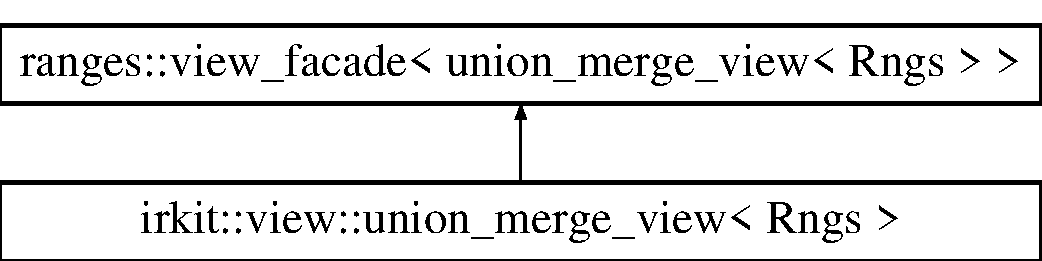
\includegraphics[height=2.000000cm]{classirkit_1_1view_1_1union__merge__view}
\end{center}
\end{figure}
\subsection*{Public Member Functions}
\begin{DoxyCompactItemize}
\item 
\hyperlink{classirkit_1_1view_1_1union__merge__view_a4a0c577e38ae0f12f3c8638911ff0e30}{union\+\_\+merge\+\_\+view} ()=default
\item 
\hyperlink{classirkit_1_1view_1_1union__merge__view_af2e80cdce25cdfd8db01a868a4dbf964}{union\+\_\+merge\+\_\+view} (Rngs rngs)
\end{DoxyCompactItemize}


\subsection{Constructor \& Destructor Documentation}
\mbox{\Hypertarget{classirkit_1_1view_1_1union__merge__view_a4a0c577e38ae0f12f3c8638911ff0e30}\label{classirkit_1_1view_1_1union__merge__view_a4a0c577e38ae0f12f3c8638911ff0e30}} 
\index{irkit\+::view\+::union\+\_\+merge\+\_\+view@{irkit\+::view\+::union\+\_\+merge\+\_\+view}!union\+\_\+merge\+\_\+view@{union\+\_\+merge\+\_\+view}}
\index{union\+\_\+merge\+\_\+view@{union\+\_\+merge\+\_\+view}!irkit\+::view\+::union\+\_\+merge\+\_\+view@{irkit\+::view\+::union\+\_\+merge\+\_\+view}}
\subsubsection{\texorpdfstring{union\+\_\+merge\+\_\+view()}{union\_merge\_view()}\hspace{0.1cm}{\footnotesize\ttfamily [1/2]}}
{\footnotesize\ttfamily template$<$class Rngs $>$ \\
\hyperlink{classirkit_1_1view_1_1union__merge__view}{irkit\+::view\+::union\+\_\+merge\+\_\+view}$<$ Rngs $>$\+::\hyperlink{classirkit_1_1view_1_1union__merge__view}{union\+\_\+merge\+\_\+view} (\begin{DoxyParamCaption}{ }\end{DoxyParamCaption})\hspace{0.3cm}{\ttfamily [default]}}

\mbox{\Hypertarget{classirkit_1_1view_1_1union__merge__view_af2e80cdce25cdfd8db01a868a4dbf964}\label{classirkit_1_1view_1_1union__merge__view_af2e80cdce25cdfd8db01a868a4dbf964}} 
\index{irkit\+::view\+::union\+\_\+merge\+\_\+view@{irkit\+::view\+::union\+\_\+merge\+\_\+view}!union\+\_\+merge\+\_\+view@{union\+\_\+merge\+\_\+view}}
\index{union\+\_\+merge\+\_\+view@{union\+\_\+merge\+\_\+view}!irkit\+::view\+::union\+\_\+merge\+\_\+view@{irkit\+::view\+::union\+\_\+merge\+\_\+view}}
\subsubsection{\texorpdfstring{union\+\_\+merge\+\_\+view()}{union\_merge\_view()}\hspace{0.1cm}{\footnotesize\ttfamily [2/2]}}
{\footnotesize\ttfamily template$<$class Rngs $>$ \\
\hyperlink{classirkit_1_1view_1_1union__merge__view}{irkit\+::view\+::union\+\_\+merge\+\_\+view}$<$ Rngs $>$\+::\hyperlink{classirkit_1_1view_1_1union__merge__view}{union\+\_\+merge\+\_\+view} (\begin{DoxyParamCaption}\item[{Rngs}]{rngs }\end{DoxyParamCaption})\hspace{0.3cm}{\ttfamily [inline]}, {\ttfamily [explicit]}}



The documentation for this class was generated from the following file\+:\begin{DoxyCompactItemize}
\item 
include/irkit/\hyperlink{view_8hpp}{view.\+hpp}\end{DoxyCompactItemize}

\hypertarget{classirkit_1_1UnionRange}{}\section{irkit\+:\+:Union\+Range$<$ Range $>$ Class Template Reference}
\label{classirkit_1_1UnionRange}\index{irkit\+::\+Union\+Range$<$ Range $>$@{irkit\+::\+Union\+Range$<$ Range $>$}}


{\ttfamily \#include $<$daat.\+hpp$>$}

\subsection*{Classes}
\begin{DoxyCompactItemize}
\item 
struct \hyperlink{structirkit_1_1UnionRange_1_1docterm}{docterm}
\begin{DoxyCompactList}\small\item\em Pair of document ID and term ID to use in D\+A\+AT term heap. \end{DoxyCompactList}\end{DoxyCompactItemize}
\subsection*{Public Member Functions}
\begin{DoxyCompactItemize}
\item 
\hyperlink{classirkit_1_1UnionRange_a23072335eaa144321314fbbdd39e9423}{Union\+Range} (const std\+::vector$<$ Range $>$ \&query\+\_\+postings, const std\+::vector$<$ \hyperlink{classirkit_1_1UnionRange_a47fb098a85581f5e33f4203e16245dae}{Score} $>$ \&weights, const std\+::vector$<$ \hyperlink{classirkit_1_1UnionRange_a47fb098a85581f5e33f4203e16245dae}{Score} $>$ \&max\+\_\+scores=std\+::move(std\+::vector$<$ \hyperlink{classirkit_1_1UnionRange_a47fb098a85581f5e33f4203e16245dae}{Score} $>$()))
\begin{DoxyCompactList}\small\item\em Creates new union range from posting lists and term weights. \end{DoxyCompactList}\item 
unsigned int \hyperlink{classirkit_1_1UnionRange_aa985f4985486d3df259be0c932340f18}{peek\+\_\+term} ()
\begin{DoxyCompactList}\small\item\em Returns the next posting\textquotesingle{}s term without advancing to the next one. \end{DoxyCompactList}\item 
\hyperlink{classirkit_1_1UnionRange_a5f694970419f5a60d7fd41d740556229}{Posting} \hyperlink{classirkit_1_1UnionRange_a5c2f9a6ec77c812febdf1778e4b9b3f6}{peek\+\_\+posting} ()
\begin{DoxyCompactList}\small\item\em Returns the next posting without advancing to the next one. \end{DoxyCompactList}\item 
\hyperlink{classirkit_1_1UnionRange_a5f694970419f5a60d7fd41d740556229}{Posting} \hyperlink{classirkit_1_1UnionRange_aedb2ab6f4a5f0b9f57cf2c55214ed42e}{next\+\_\+posting} ()
\begin{DoxyCompactList}\small\item\em Returns the next posting in sorted union order. \end{DoxyCompactList}\item 
\hyperlink{classirkit_1_1UnionRange_a5f694970419f5a60d7fd41d740556229}{Posting} \hyperlink{classirkit_1_1UnionRange_a9161a468e74df4e76cd04104763f7d97}{next\+\_\+doc} ()
\begin{DoxyCompactList}\small\item\em Returns the next {\itshape accumulated posting} in sorted union order. \end{DoxyCompactList}\item 
std\+::vector$<$ \hyperlink{structirkit_1_1UnionRange_1_1docterm}{docterm} $>$ \hyperlink{classirkit_1_1UnionRange_aacb1050fb1d624260c4013f4ba1939a6}{select\+\_\+pivot} (\hyperlink{classirkit_1_1UnionRange_a47fb098a85581f5e33f4203e16245dae}{Score} threshold)
\item 
\hyperlink{classirkit_1_1UnionRange_a5f694970419f5a60d7fd41d740556229}{Posting} \hyperlink{classirkit_1_1UnionRange_a6f6bf3aa9d7d273371a9477b88c54737}{next\+\_\+doc\+\_\+wand} (\hyperlink{classirkit_1_1UnionRange_a47fb098a85581f5e33f4203e16245dae}{Score} threshold)
\item 
bool \hyperlink{classirkit_1_1UnionRange_af12b028d791c9d9821c17ae30084fa86}{empty} () const
\begin{DoxyCompactList}\small\item\em Returns true if no further postings are available. \end{DoxyCompactList}\end{DoxyCompactItemize}
\subsection*{Protected Types}
\begin{DoxyCompactItemize}
\item 
using \hyperlink{classirkit_1_1UnionRange_a5f694970419f5a60d7fd41d740556229}{Posting} = \hyperlink{namespaceirkit_afcffab67300c5c703cb38a363c9a6f1d}{pure\+\_\+element\+\_\+t}$<$ Range $>$
\item 
using \hyperlink{classirkit_1_1UnionRange_a47fb098a85581f5e33f4203e16245dae}{Score} = \hyperlink{namespaceirkit_a754dabe3346f950c948e7596d9d46c71}{score\+\_\+t}$<$ \hyperlink{classirkit_1_1UnionRange_a5f694970419f5a60d7fd41d740556229}{Posting} $>$
\item 
using \hyperlink{classirkit_1_1UnionRange_a387589b1f09868b60485c4ab8c61f97a}{Doc} = \hyperlink{namespaceirkit_a595d83053e112c98ab2a1b65e5dd74be}{doc\+\_\+t}$<$ \hyperlink{classirkit_1_1UnionRange_a5f694970419f5a60d7fd41d740556229}{Posting} $>$
\end{DoxyCompactItemize}
\subsection*{Protected Member Functions}
\begin{DoxyCompactItemize}
\item 
void \hyperlink{classirkit_1_1UnionRange_aabdf133213056f20e0526c6736dbff3e}{init} (const std\+::vector$<$ Range $>$ \&query\+\_\+postings)
\begin{DoxyCompactList}\small\item\em Initilizes moving ranges and heap. \end{DoxyCompactList}\item 
void \hyperlink{classirkit_1_1UnionRange_ab0548ed7d94aece8f72d0ca4db65b456}{nextge} (unsigned int term, \hyperlink{classirkit_1_1UnionRange_a387589b1f09868b60485c4ab8c61f97a}{Doc} doc)
\end{DoxyCompactItemize}
\subsection*{Protected Attributes}
\begin{DoxyCompactItemize}
\item 
const std\+::vector$<$ \hyperlink{classirkit_1_1UnionRange_a47fb098a85581f5e33f4203e16245dae}{Score} $>$ \& \hyperlink{classirkit_1_1UnionRange_a0c53eb9b1c9e8aa18621f4c129a6ff90}{weights\+\_\+}
\item 
const std\+::vector$<$ \hyperlink{classirkit_1_1UnionRange_a47fb098a85581f5e33f4203e16245dae}{Score} $>$ \& \hyperlink{classirkit_1_1UnionRange_a980f7cfaf14c7c4d93b13b6d7ce6a859}{max\+\_\+scores\+\_\+}
\item 
std\+::vector$<$ \hyperlink{structirkit_1_1moving__range}{moving\+\_\+range}$<$ \hyperlink{namespaceirkit_a4b1668583041117eb42c1b5a1091b804}{const\+\_\+iterator\+\_\+t}$<$ Range $>$ $>$ $>$ \hyperlink{classirkit_1_1UnionRange_acb9b9e969f1c90bb18bf1e4eb99f124b}{ranges\+\_\+}
\item 
std\+::vector$<$ \hyperlink{structirkit_1_1UnionRange_1_1docterm}{docterm} $>$ \hyperlink{classirkit_1_1UnionRange_a613eebb9b7b8601bffdad1d842c8c7f0}{heap\+\_\+}
\end{DoxyCompactItemize}


\subsection{Detailed Description}
\subsubsection*{template$<$class Range$>$\newline
class irkit\+::\+Union\+Range$<$ Range $>$}

Represents the union of sorted ranges (posting lists). T\+O\+DO\+: Generalize. T\+O\+DO\+: Improve efficiency below 17 ms on Bo\+VW. 

\subsection{Member Typedef Documentation}
\mbox{\Hypertarget{classirkit_1_1UnionRange_a387589b1f09868b60485c4ab8c61f97a}\label{classirkit_1_1UnionRange_a387589b1f09868b60485c4ab8c61f97a}} 
\index{irkit\+::\+Union\+Range@{irkit\+::\+Union\+Range}!Doc@{Doc}}
\index{Doc@{Doc}!irkit\+::\+Union\+Range@{irkit\+::\+Union\+Range}}
\subsubsection{\texorpdfstring{Doc}{Doc}}
{\footnotesize\ttfamily template$<$class Range $>$ \\
using \hyperlink{classirkit_1_1UnionRange}{irkit\+::\+Union\+Range}$<$ Range $>$\+::\hyperlink{classirkit_1_1UnionRange_a387589b1f09868b60485c4ab8c61f97a}{Doc} =  \hyperlink{namespaceirkit_a595d83053e112c98ab2a1b65e5dd74be}{doc\+\_\+t}$<$\hyperlink{classirkit_1_1UnionRange_a5f694970419f5a60d7fd41d740556229}{Posting}$>$\hspace{0.3cm}{\ttfamily [protected]}}

\mbox{\Hypertarget{classirkit_1_1UnionRange_a5f694970419f5a60d7fd41d740556229}\label{classirkit_1_1UnionRange_a5f694970419f5a60d7fd41d740556229}} 
\index{irkit\+::\+Union\+Range@{irkit\+::\+Union\+Range}!Posting@{Posting}}
\index{Posting@{Posting}!irkit\+::\+Union\+Range@{irkit\+::\+Union\+Range}}
\subsubsection{\texorpdfstring{Posting}{Posting}}
{\footnotesize\ttfamily template$<$class Range $>$ \\
using \hyperlink{classirkit_1_1UnionRange}{irkit\+::\+Union\+Range}$<$ Range $>$\+::\hyperlink{classirkit_1_1UnionRange_a5f694970419f5a60d7fd41d740556229}{Posting} =  \hyperlink{namespaceirkit_afcffab67300c5c703cb38a363c9a6f1d}{pure\+\_\+element\+\_\+t}$<$Range$>$\hspace{0.3cm}{\ttfamily [protected]}}

\mbox{\Hypertarget{classirkit_1_1UnionRange_a47fb098a85581f5e33f4203e16245dae}\label{classirkit_1_1UnionRange_a47fb098a85581f5e33f4203e16245dae}} 
\index{irkit\+::\+Union\+Range@{irkit\+::\+Union\+Range}!Score@{Score}}
\index{Score@{Score}!irkit\+::\+Union\+Range@{irkit\+::\+Union\+Range}}
\subsubsection{\texorpdfstring{Score}{Score}}
{\footnotesize\ttfamily template$<$class Range $>$ \\
using \hyperlink{classirkit_1_1UnionRange}{irkit\+::\+Union\+Range}$<$ Range $>$\+::\hyperlink{classirkit_1_1UnionRange_a47fb098a85581f5e33f4203e16245dae}{Score} =  \hyperlink{namespaceirkit_a754dabe3346f950c948e7596d9d46c71}{score\+\_\+t}$<$\hyperlink{classirkit_1_1UnionRange_a5f694970419f5a60d7fd41d740556229}{Posting}$>$\hspace{0.3cm}{\ttfamily [protected]}}



\subsection{Constructor \& Destructor Documentation}
\mbox{\Hypertarget{classirkit_1_1UnionRange_a23072335eaa144321314fbbdd39e9423}\label{classirkit_1_1UnionRange_a23072335eaa144321314fbbdd39e9423}} 
\index{irkit\+::\+Union\+Range@{irkit\+::\+Union\+Range}!Union\+Range@{Union\+Range}}
\index{Union\+Range@{Union\+Range}!irkit\+::\+Union\+Range@{irkit\+::\+Union\+Range}}
\subsubsection{\texorpdfstring{Union\+Range()}{UnionRange()}}
{\footnotesize\ttfamily template$<$class Range $>$ \\
\hyperlink{classirkit_1_1UnionRange}{irkit\+::\+Union\+Range}$<$ Range $>$\+::\hyperlink{classirkit_1_1UnionRange}{Union\+Range} (\begin{DoxyParamCaption}\item[{const std\+::vector$<$ Range $>$ \&}]{query\+\_\+postings,  }\item[{const std\+::vector$<$ \hyperlink{classirkit_1_1UnionRange_a47fb098a85581f5e33f4203e16245dae}{Score} $>$ \&}]{weights,  }\item[{const std\+::vector$<$ \hyperlink{classirkit_1_1UnionRange_a47fb098a85581f5e33f4203e16245dae}{Score} $>$ \&}]{max\+\_\+scores = {\ttfamily std\+:\+:move(std\+:\+:vector$<$\hyperlink{classirkit_1_1UnionRange_a47fb098a85581f5e33f4203e16245dae}{Score}$>$())} }\end{DoxyParamCaption})\hspace{0.3cm}{\ttfamily [inline]}}



Creates new union range from posting lists and term weights. 

\begin{DoxyPrecond}{Precondition}
Each posting list must be sorted by increasing document I\+Ds. 
\end{DoxyPrecond}

\begin{DoxyParams}{Parameters}
{\em query\+\_\+postings} & a vector of posting lists for all query terms \\
\hline
{\em weights} & a vector of term weights \\
\hline
\end{DoxyParams}


\subsection{Member Function Documentation}
\mbox{\Hypertarget{classirkit_1_1UnionRange_af12b028d791c9d9821c17ae30084fa86}\label{classirkit_1_1UnionRange_af12b028d791c9d9821c17ae30084fa86}} 
\index{irkit\+::\+Union\+Range@{irkit\+::\+Union\+Range}!empty@{empty}}
\index{empty@{empty}!irkit\+::\+Union\+Range@{irkit\+::\+Union\+Range}}
\subsubsection{\texorpdfstring{empty()}{empty()}}
{\footnotesize\ttfamily template$<$class Range $>$ \\
bool \hyperlink{classirkit_1_1UnionRange}{irkit\+::\+Union\+Range}$<$ Range $>$\+::empty (\begin{DoxyParamCaption}{ }\end{DoxyParamCaption}) const\hspace{0.3cm}{\ttfamily [inline]}}



Returns true if no further postings are available. 

\mbox{\Hypertarget{classirkit_1_1UnionRange_aabdf133213056f20e0526c6736dbff3e}\label{classirkit_1_1UnionRange_aabdf133213056f20e0526c6736dbff3e}} 
\index{irkit\+::\+Union\+Range@{irkit\+::\+Union\+Range}!init@{init}}
\index{init@{init}!irkit\+::\+Union\+Range@{irkit\+::\+Union\+Range}}
\subsubsection{\texorpdfstring{init()}{init()}}
{\footnotesize\ttfamily template$<$class Range $>$ \\
void \hyperlink{classirkit_1_1UnionRange}{irkit\+::\+Union\+Range}$<$ Range $>$\+::init (\begin{DoxyParamCaption}\item[{const std\+::vector$<$ Range $>$ \&}]{query\+\_\+postings }\end{DoxyParamCaption})\hspace{0.3cm}{\ttfamily [inline]}, {\ttfamily [protected]}}



Initilizes moving ranges and heap. 

\mbox{\Hypertarget{classirkit_1_1UnionRange_a9161a468e74df4e76cd04104763f7d97}\label{classirkit_1_1UnionRange_a9161a468e74df4e76cd04104763f7d97}} 
\index{irkit\+::\+Union\+Range@{irkit\+::\+Union\+Range}!next\+\_\+doc@{next\+\_\+doc}}
\index{next\+\_\+doc@{next\+\_\+doc}!irkit\+::\+Union\+Range@{irkit\+::\+Union\+Range}}
\subsubsection{\texorpdfstring{next\+\_\+doc()}{next\_doc()}}
{\footnotesize\ttfamily template$<$class Range $>$ \\
\hyperlink{classirkit_1_1UnionRange_a5f694970419f5a60d7fd41d740556229}{Posting} \hyperlink{classirkit_1_1UnionRange}{irkit\+::\+Union\+Range}$<$ Range $>$\+::next\+\_\+doc (\begin{DoxyParamCaption}{ }\end{DoxyParamCaption})\hspace{0.3cm}{\ttfamily [inline]}}



Returns the next {\itshape accumulated posting} in sorted union order. 

An accumulated posting is an object of the same type as posting, but its score is a sum of all the partial scores for the next available document.

Note that if {\itshape next\+\_\+posting} is invoked independently, this will either return an incorrect score or will skip a document (or documents). \mbox{\Hypertarget{classirkit_1_1UnionRange_a6f6bf3aa9d7d273371a9477b88c54737}\label{classirkit_1_1UnionRange_a6f6bf3aa9d7d273371a9477b88c54737}} 
\index{irkit\+::\+Union\+Range@{irkit\+::\+Union\+Range}!next\+\_\+doc\+\_\+wand@{next\+\_\+doc\+\_\+wand}}
\index{next\+\_\+doc\+\_\+wand@{next\+\_\+doc\+\_\+wand}!irkit\+::\+Union\+Range@{irkit\+::\+Union\+Range}}
\subsubsection{\texorpdfstring{next\+\_\+doc\+\_\+wand()}{next\_doc\_wand()}}
{\footnotesize\ttfamily template$<$class Range $>$ \\
\hyperlink{classirkit_1_1UnionRange_a5f694970419f5a60d7fd41d740556229}{Posting} \hyperlink{classirkit_1_1UnionRange}{irkit\+::\+Union\+Range}$<$ Range $>$\+::next\+\_\+doc\+\_\+wand (\begin{DoxyParamCaption}\item[{\hyperlink{classirkit_1_1UnionRange_a47fb098a85581f5e33f4203e16245dae}{Score}}]{threshold }\end{DoxyParamCaption})\hspace{0.3cm}{\ttfamily [inline]}}

\mbox{\Hypertarget{classirkit_1_1UnionRange_aedb2ab6f4a5f0b9f57cf2c55214ed42e}\label{classirkit_1_1UnionRange_aedb2ab6f4a5f0b9f57cf2c55214ed42e}} 
\index{irkit\+::\+Union\+Range@{irkit\+::\+Union\+Range}!next\+\_\+posting@{next\+\_\+posting}}
\index{next\+\_\+posting@{next\+\_\+posting}!irkit\+::\+Union\+Range@{irkit\+::\+Union\+Range}}
\subsubsection{\texorpdfstring{next\+\_\+posting()}{next\_posting()}}
{\footnotesize\ttfamily template$<$class Range $>$ \\
\hyperlink{classirkit_1_1UnionRange_a5f694970419f5a60d7fd41d740556229}{Posting} \hyperlink{classirkit_1_1UnionRange}{irkit\+::\+Union\+Range}$<$ Range $>$\+::next\+\_\+posting (\begin{DoxyParamCaption}{ }\end{DoxyParamCaption})\hspace{0.3cm}{\ttfamily [inline]}}



Returns the next posting in sorted union order. 

\mbox{\Hypertarget{classirkit_1_1UnionRange_ab0548ed7d94aece8f72d0ca4db65b456}\label{classirkit_1_1UnionRange_ab0548ed7d94aece8f72d0ca4db65b456}} 
\index{irkit\+::\+Union\+Range@{irkit\+::\+Union\+Range}!nextge@{nextge}}
\index{nextge@{nextge}!irkit\+::\+Union\+Range@{irkit\+::\+Union\+Range}}
\subsubsection{\texorpdfstring{nextge()}{nextge()}}
{\footnotesize\ttfamily template$<$class Range $>$ \\
void \hyperlink{classirkit_1_1UnionRange}{irkit\+::\+Union\+Range}$<$ Range $>$\+::nextge (\begin{DoxyParamCaption}\item[{unsigned int}]{term,  }\item[{\hyperlink{classirkit_1_1UnionRange_a387589b1f09868b60485c4ab8c61f97a}{Doc}}]{doc }\end{DoxyParamCaption})\hspace{0.3cm}{\ttfamily [inline]}, {\ttfamily [protected]}}

\mbox{\Hypertarget{classirkit_1_1UnionRange_a5c2f9a6ec77c812febdf1778e4b9b3f6}\label{classirkit_1_1UnionRange_a5c2f9a6ec77c812febdf1778e4b9b3f6}} 
\index{irkit\+::\+Union\+Range@{irkit\+::\+Union\+Range}!peek\+\_\+posting@{peek\+\_\+posting}}
\index{peek\+\_\+posting@{peek\+\_\+posting}!irkit\+::\+Union\+Range@{irkit\+::\+Union\+Range}}
\subsubsection{\texorpdfstring{peek\+\_\+posting()}{peek\_posting()}}
{\footnotesize\ttfamily template$<$class Range $>$ \\
\hyperlink{classirkit_1_1UnionRange_a5f694970419f5a60d7fd41d740556229}{Posting} \hyperlink{classirkit_1_1UnionRange}{irkit\+::\+Union\+Range}$<$ Range $>$\+::peek\+\_\+posting (\begin{DoxyParamCaption}{ }\end{DoxyParamCaption})\hspace{0.3cm}{\ttfamily [inline]}}



Returns the next posting without advancing to the next one. 

\mbox{\Hypertarget{classirkit_1_1UnionRange_aa985f4985486d3df259be0c932340f18}\label{classirkit_1_1UnionRange_aa985f4985486d3df259be0c932340f18}} 
\index{irkit\+::\+Union\+Range@{irkit\+::\+Union\+Range}!peek\+\_\+term@{peek\+\_\+term}}
\index{peek\+\_\+term@{peek\+\_\+term}!irkit\+::\+Union\+Range@{irkit\+::\+Union\+Range}}
\subsubsection{\texorpdfstring{peek\+\_\+term()}{peek\_term()}}
{\footnotesize\ttfamily template$<$class Range $>$ \\
unsigned int \hyperlink{classirkit_1_1UnionRange}{irkit\+::\+Union\+Range}$<$ Range $>$\+::peek\+\_\+term (\begin{DoxyParamCaption}{ }\end{DoxyParamCaption})\hspace{0.3cm}{\ttfamily [inline]}}



Returns the next posting\textquotesingle{}s term without advancing to the next one. 

\mbox{\Hypertarget{classirkit_1_1UnionRange_aacb1050fb1d624260c4013f4ba1939a6}\label{classirkit_1_1UnionRange_aacb1050fb1d624260c4013f4ba1939a6}} 
\index{irkit\+::\+Union\+Range@{irkit\+::\+Union\+Range}!select\+\_\+pivot@{select\+\_\+pivot}}
\index{select\+\_\+pivot@{select\+\_\+pivot}!irkit\+::\+Union\+Range@{irkit\+::\+Union\+Range}}
\subsubsection{\texorpdfstring{select\+\_\+pivot()}{select\_pivot()}}
{\footnotesize\ttfamily template$<$class Range $>$ \\
std\+::vector$<$\hyperlink{structirkit_1_1UnionRange_1_1docterm}{docterm}$>$ \hyperlink{classirkit_1_1UnionRange}{irkit\+::\+Union\+Range}$<$ Range $>$\+::select\+\_\+pivot (\begin{DoxyParamCaption}\item[{\hyperlink{classirkit_1_1UnionRange_a47fb098a85581f5e33f4203e16245dae}{Score}}]{threshold }\end{DoxyParamCaption})\hspace{0.3cm}{\ttfamily [inline]}}

Returns the docterm entries for all terms preceding (and including) pivot. 

\subsection{Member Data Documentation}
\mbox{\Hypertarget{classirkit_1_1UnionRange_a613eebb9b7b8601bffdad1d842c8c7f0}\label{classirkit_1_1UnionRange_a613eebb9b7b8601bffdad1d842c8c7f0}} 
\index{irkit\+::\+Union\+Range@{irkit\+::\+Union\+Range}!heap\+\_\+@{heap\+\_\+}}
\index{heap\+\_\+@{heap\+\_\+}!irkit\+::\+Union\+Range@{irkit\+::\+Union\+Range}}
\subsubsection{\texorpdfstring{heap\+\_\+}{heap\_}}
{\footnotesize\ttfamily template$<$class Range $>$ \\
std\+::vector$<$\hyperlink{structirkit_1_1UnionRange_1_1docterm}{docterm}$>$ \hyperlink{classirkit_1_1UnionRange}{irkit\+::\+Union\+Range}$<$ Range $>$\+::heap\+\_\+\hspace{0.3cm}{\ttfamily [protected]}}

\mbox{\Hypertarget{classirkit_1_1UnionRange_a980f7cfaf14c7c4d93b13b6d7ce6a859}\label{classirkit_1_1UnionRange_a980f7cfaf14c7c4d93b13b6d7ce6a859}} 
\index{irkit\+::\+Union\+Range@{irkit\+::\+Union\+Range}!max\+\_\+scores\+\_\+@{max\+\_\+scores\+\_\+}}
\index{max\+\_\+scores\+\_\+@{max\+\_\+scores\+\_\+}!irkit\+::\+Union\+Range@{irkit\+::\+Union\+Range}}
\subsubsection{\texorpdfstring{max\+\_\+scores\+\_\+}{max\_scores\_}}
{\footnotesize\ttfamily template$<$class Range $>$ \\
const std\+::vector$<$\hyperlink{classirkit_1_1UnionRange_a47fb098a85581f5e33f4203e16245dae}{Score}$>$\& \hyperlink{classirkit_1_1UnionRange}{irkit\+::\+Union\+Range}$<$ Range $>$\+::max\+\_\+scores\+\_\+\hspace{0.3cm}{\ttfamily [protected]}}

\mbox{\Hypertarget{classirkit_1_1UnionRange_acb9b9e969f1c90bb18bf1e4eb99f124b}\label{classirkit_1_1UnionRange_acb9b9e969f1c90bb18bf1e4eb99f124b}} 
\index{irkit\+::\+Union\+Range@{irkit\+::\+Union\+Range}!ranges\+\_\+@{ranges\+\_\+}}
\index{ranges\+\_\+@{ranges\+\_\+}!irkit\+::\+Union\+Range@{irkit\+::\+Union\+Range}}
\subsubsection{\texorpdfstring{ranges\+\_\+}{ranges\_}}
{\footnotesize\ttfamily template$<$class Range $>$ \\
std\+::vector$<$\hyperlink{structirkit_1_1moving__range}{moving\+\_\+range}$<$\hyperlink{namespaceirkit_a4b1668583041117eb42c1b5a1091b804}{const\+\_\+iterator\+\_\+t}$<$Range$>$ $>$ $>$ \hyperlink{classirkit_1_1UnionRange}{irkit\+::\+Union\+Range}$<$ Range $>$\+::ranges\+\_\+\hspace{0.3cm}{\ttfamily [protected]}}

\mbox{\Hypertarget{classirkit_1_1UnionRange_a0c53eb9b1c9e8aa18621f4c129a6ff90}\label{classirkit_1_1UnionRange_a0c53eb9b1c9e8aa18621f4c129a6ff90}} 
\index{irkit\+::\+Union\+Range@{irkit\+::\+Union\+Range}!weights\+\_\+@{weights\+\_\+}}
\index{weights\+\_\+@{weights\+\_\+}!irkit\+::\+Union\+Range@{irkit\+::\+Union\+Range}}
\subsubsection{\texorpdfstring{weights\+\_\+}{weights\_}}
{\footnotesize\ttfamily template$<$class Range $>$ \\
const std\+::vector$<$\hyperlink{classirkit_1_1UnionRange_a47fb098a85581f5e33f4203e16245dae}{Score}$>$\& \hyperlink{classirkit_1_1UnionRange}{irkit\+::\+Union\+Range}$<$ Range $>$\+::weights\+\_\+\hspace{0.3cm}{\ttfamily [protected]}}



The documentation for this class was generated from the following file\+:\begin{DoxyCompactItemize}
\item 
include/irkit/\hyperlink{daat_8hpp}{daat.\+hpp}\end{DoxyCompactItemize}

\hypertarget{classbloodhound_1_1query_1_1WandRetriever}{}\section{bloodhound\+:\+:query\+:\+:Wand\+Retriever$<$ Posting\+List $>$ Class Template Reference}
\label{classbloodhound_1_1query_1_1WandRetriever}\index{bloodhound\+::query\+::\+Wand\+Retriever$<$ Posting\+List $>$@{bloodhound\+::query\+::\+Wand\+Retriever$<$ Posting\+List $>$}}


W\+A\+ND (Weak-\/\+A\+ND) query retriever.  




{\ttfamily \#include $<$retrievers.\+hpp$>$}

Inheritance diagram for bloodhound\+:\+:query\+:\+:Wand\+Retriever$<$ Posting\+List $>$\+:\begin{figure}[H]
\begin{center}
\leavevmode
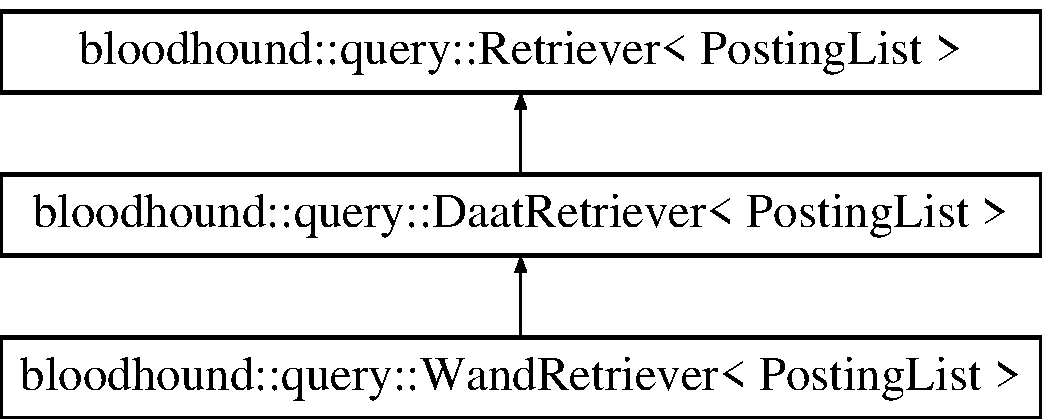
\includegraphics[height=3.000000cm]{classbloodhound_1_1query_1_1WandRetriever}
\end{center}
\end{figure}
\subsection*{Public Member Functions}
\begin{DoxyCompactItemize}
\item 
virtual std\+::vector$<$ \mbox{\hyperlink{structbloodhound_1_1query_1_1Result}{Result}} $>$ \mbox{\hyperlink{classbloodhound_1_1query_1_1WandRetriever_a5f3068bc363c16c5b7255a925ea5af8c}{retrieve}} (const std\+::vector$<$ \mbox{\hyperlink{classbloodhound_1_1PostingList}{Posting\+List}} $>$ \&term\+\_\+postings, const std\+::vector$<$ \mbox{\hyperlink{structbloodhound_1_1Score}{Score}} $>$ \&term\+\_\+weights, std\+::size\+\_\+t k)
\begin{DoxyCompactList}\small\item\em Retrieves top-\/k results for the given posting lists and term weights. \end{DoxyCompactList}\item 
virtual nlohmann\+::json \mbox{\hyperlink{classbloodhound_1_1query_1_1WandRetriever_a1e593c2cddb2ca4f2415c59ca26e6a36}{stats}} ()
\end{DoxyCompactItemize}


\subsection{Detailed Description}
\subsubsection*{template$<$typename Posting\+List$>$\newline
class bloodhound\+::query\+::\+Wand\+Retriever$<$ Posting\+List $>$}

W\+A\+ND (Weak-\/\+A\+ND) query retriever. 

\subsection{Member Function Documentation}
\mbox{\Hypertarget{classbloodhound_1_1query_1_1WandRetriever_a5f3068bc363c16c5b7255a925ea5af8c}\label{classbloodhound_1_1query_1_1WandRetriever_a5f3068bc363c16c5b7255a925ea5af8c}} 
\index{bloodhound\+::query\+::\+Wand\+Retriever@{bloodhound\+::query\+::\+Wand\+Retriever}!retrieve@{retrieve}}
\index{retrieve@{retrieve}!bloodhound\+::query\+::\+Wand\+Retriever@{bloodhound\+::query\+::\+Wand\+Retriever}}
\subsubsection{\texorpdfstring{retrieve()}{retrieve()}}
{\footnotesize\ttfamily template$<$typename Posting\+List $>$ \\
virtual std\+::vector$<$\mbox{\hyperlink{structbloodhound_1_1query_1_1Result}{Result}}$>$ \mbox{\hyperlink{classbloodhound_1_1query_1_1WandRetriever}{bloodhound\+::query\+::\+Wand\+Retriever}}$<$ \mbox{\hyperlink{classbloodhound_1_1PostingList}{Posting\+List}} $>$\+::retrieve (\begin{DoxyParamCaption}\item[{const std\+::vector$<$ \mbox{\hyperlink{classbloodhound_1_1PostingList}{Posting\+List}} $>$ \&}]{term\+\_\+postings,  }\item[{const std\+::vector$<$ \mbox{\hyperlink{structbloodhound_1_1Score}{Score}} $>$ \&}]{term\+\_\+weights,  }\item[{std\+::size\+\_\+t}]{k }\end{DoxyParamCaption})\hspace{0.3cm}{\ttfamily [inline]}, {\ttfamily [virtual]}}



Retrieves top-\/k results for the given posting lists and term weights. 



Reimplemented from \mbox{\hyperlink{classbloodhound_1_1query_1_1DaatRetriever_ab80b4867fc263827dc2fdbe0965a2e8c}{bloodhound\+::query\+::\+Daat\+Retriever$<$ Posting\+List $>$}}.

\mbox{\Hypertarget{classbloodhound_1_1query_1_1WandRetriever_a1e593c2cddb2ca4f2415c59ca26e6a36}\label{classbloodhound_1_1query_1_1WandRetriever_a1e593c2cddb2ca4f2415c59ca26e6a36}} 
\index{bloodhound\+::query\+::\+Wand\+Retriever@{bloodhound\+::query\+::\+Wand\+Retriever}!stats@{stats}}
\index{stats@{stats}!bloodhound\+::query\+::\+Wand\+Retriever@{bloodhound\+::query\+::\+Wand\+Retriever}}
\subsubsection{\texorpdfstring{stats()}{stats()}}
{\footnotesize\ttfamily template$<$typename Posting\+List $>$ \\
virtual nlohmann\+::json \mbox{\hyperlink{classbloodhound_1_1query_1_1WandRetriever}{bloodhound\+::query\+::\+Wand\+Retriever}}$<$ \mbox{\hyperlink{classbloodhound_1_1PostingList}{Posting\+List}} $>$\+::stats (\begin{DoxyParamCaption}{ }\end{DoxyParamCaption})\hspace{0.3cm}{\ttfamily [inline]}, {\ttfamily [virtual]}}



Reimplemented from \mbox{\hyperlink{classbloodhound_1_1query_1_1Retriever_a58da32a5139b980ba874f8b5e6bb89ec}{bloodhound\+::query\+::\+Retriever$<$ Posting\+List $>$}}.



The documentation for this class was generated from the following file\+:\begin{DoxyCompactItemize}
\item 
include/\mbox{\hyperlink{retrievers_8hpp}{retrievers.\+hpp}}\end{DoxyCompactItemize}

\hypertarget{classirkit_1_1view_1_1ZipView}{}\section{irkit\+:\+:view\+:\+:Zip\+View$<$ Zip\+Fn, Left\+Range, Right\+Range $>$ Class Template Reference}
\label{classirkit_1_1view_1_1ZipView}\index{irkit\+::view\+::\+Zip\+View$<$ Zip\+Fn, Left\+Range, Right\+Range $>$@{irkit\+::view\+::\+Zip\+View$<$ Zip\+Fn, Left\+Range, Right\+Range $>$}}


A zip view of two ranges.  




{\ttfamily \#include $<$utils.\+hpp$>$}

\subsection*{Classes}
\begin{DoxyCompactItemize}
\item 
class \hyperlink{classirkit_1_1view_1_1ZipView_1_1const__iterator}{const\+\_\+iterator}
\end{DoxyCompactItemize}
\subsection*{Public Member Functions}
\begin{DoxyCompactItemize}
\item 
\hyperlink{classirkit_1_1view_1_1ZipView_a581e90890462717bbdac0f02dc343641}{Zip\+View} (const Left\+Range \&left, const Right\+Range \&right, Zip\+Fn zip\+\_\+fn)
\begin{DoxyCompactList}\small\item\em Constructs a zip view. \end{DoxyCompactList}\item 
\hyperlink{classirkit_1_1view_1_1ZipView_1_1const__iterator}{const\+\_\+iterator} \hyperlink{classirkit_1_1view_1_1ZipView_ab92e5ce12bcf45a9a797294d5b2e97e7}{cbegin} () const
\item 
\hyperlink{classirkit_1_1view_1_1ZipView_1_1const__iterator}{const\+\_\+iterator} \hyperlink{classirkit_1_1view_1_1ZipView_a5ba1f0456da3ffc049e59418b4a01a3f}{cend} () const
\item 
\hyperlink{classirkit_1_1view_1_1ZipView_1_1const__iterator}{const\+\_\+iterator} \hyperlink{classirkit_1_1view_1_1ZipView_af278d23b14dd71c1c5d7e145a5d0771b}{begin} () const
\item 
\hyperlink{classirkit_1_1view_1_1ZipView_1_1const__iterator}{const\+\_\+iterator} \hyperlink{classirkit_1_1view_1_1ZipView_ab8a193bad7c33b93367014f32e9cf360}{end} () const
\end{DoxyCompactItemize}


\subsection{Detailed Description}
\subsubsection*{template$<$class Zip\+Fn, class Left\+Range, class Right\+Range$>$\newline
class irkit\+::view\+::\+Zip\+View$<$ Zip\+Fn, Left\+Range, Right\+Range $>$}

A zip view of two ranges. 


\begin{DoxyTemplParams}{Template Parameters}
{\em Zip\+Fn} & A function type for element generation. \\
\hline
{\em Left\+Range} & The type of the left range. \\
\hline
{\em Right\+Range} & The type of the right range. \\
\hline
\end{DoxyTemplParams}


\subsection{Constructor \& Destructor Documentation}
\mbox{\Hypertarget{classirkit_1_1view_1_1ZipView_a581e90890462717bbdac0f02dc343641}\label{classirkit_1_1view_1_1ZipView_a581e90890462717bbdac0f02dc343641}} 
\index{irkit\+::view\+::\+Zip\+View@{irkit\+::view\+::\+Zip\+View}!Zip\+View@{Zip\+View}}
\index{Zip\+View@{Zip\+View}!irkit\+::view\+::\+Zip\+View@{irkit\+::view\+::\+Zip\+View}}
\subsubsection{\texorpdfstring{Zip\+View()}{ZipView()}}
{\footnotesize\ttfamily template$<$class Zip\+Fn , class Left\+Range , class Right\+Range $>$ \\
\hyperlink{classirkit_1_1view_1_1ZipView}{irkit\+::view\+::\+Zip\+View}$<$ Zip\+Fn, Left\+Range, Right\+Range $>$\+::\hyperlink{classirkit_1_1view_1_1ZipView}{Zip\+View} (\begin{DoxyParamCaption}\item[{const Left\+Range \&}]{left,  }\item[{const Right\+Range \&}]{right,  }\item[{Zip\+Fn}]{zip\+\_\+fn }\end{DoxyParamCaption})\hspace{0.3cm}{\ttfamily [inline]}}



Constructs a zip view. 


\begin{DoxyParams}{Parameters}
{\em left} & The left range. \\
\hline
{\em right} & The right range. \\
\hline
{\em zip\+\_\+fn} & A function which, given an element of {\ttfamily left} and an element of {\ttfamily right}, returns an element of the zipped view.\\
\hline
\end{DoxyParams}
Instead of using the constructor directly, rather use \hyperlink{namespaceirkit_1_1view_ad4847c0d8f90f3c8854994d3289d51d6}{zip()} function. 

\subsection{Member Function Documentation}
\mbox{\Hypertarget{classirkit_1_1view_1_1ZipView_af278d23b14dd71c1c5d7e145a5d0771b}\label{classirkit_1_1view_1_1ZipView_af278d23b14dd71c1c5d7e145a5d0771b}} 
\index{irkit\+::view\+::\+Zip\+View@{irkit\+::view\+::\+Zip\+View}!begin@{begin}}
\index{begin@{begin}!irkit\+::view\+::\+Zip\+View@{irkit\+::view\+::\+Zip\+View}}
\subsubsection{\texorpdfstring{begin()}{begin()}}
{\footnotesize\ttfamily template$<$class Zip\+Fn , class Left\+Range , class Right\+Range $>$ \\
\hyperlink{classirkit_1_1view_1_1ZipView_1_1const__iterator}{const\+\_\+iterator} \hyperlink{classirkit_1_1view_1_1ZipView}{irkit\+::view\+::\+Zip\+View}$<$ Zip\+Fn, Left\+Range, Right\+Range $>$\+::begin (\begin{DoxyParamCaption}{ }\end{DoxyParamCaption}) const\hspace{0.3cm}{\ttfamily [inline]}}

\mbox{\Hypertarget{classirkit_1_1view_1_1ZipView_ab92e5ce12bcf45a9a797294d5b2e97e7}\label{classirkit_1_1view_1_1ZipView_ab92e5ce12bcf45a9a797294d5b2e97e7}} 
\index{irkit\+::view\+::\+Zip\+View@{irkit\+::view\+::\+Zip\+View}!cbegin@{cbegin}}
\index{cbegin@{cbegin}!irkit\+::view\+::\+Zip\+View@{irkit\+::view\+::\+Zip\+View}}
\subsubsection{\texorpdfstring{cbegin()}{cbegin()}}
{\footnotesize\ttfamily template$<$class Zip\+Fn , class Left\+Range , class Right\+Range $>$ \\
\hyperlink{classirkit_1_1view_1_1ZipView_1_1const__iterator}{const\+\_\+iterator} \hyperlink{classirkit_1_1view_1_1ZipView}{irkit\+::view\+::\+Zip\+View}$<$ Zip\+Fn, Left\+Range, Right\+Range $>$\+::cbegin (\begin{DoxyParamCaption}{ }\end{DoxyParamCaption}) const\hspace{0.3cm}{\ttfamily [inline]}}

\mbox{\Hypertarget{classirkit_1_1view_1_1ZipView_a5ba1f0456da3ffc049e59418b4a01a3f}\label{classirkit_1_1view_1_1ZipView_a5ba1f0456da3ffc049e59418b4a01a3f}} 
\index{irkit\+::view\+::\+Zip\+View@{irkit\+::view\+::\+Zip\+View}!cend@{cend}}
\index{cend@{cend}!irkit\+::view\+::\+Zip\+View@{irkit\+::view\+::\+Zip\+View}}
\subsubsection{\texorpdfstring{cend()}{cend()}}
{\footnotesize\ttfamily template$<$class Zip\+Fn , class Left\+Range , class Right\+Range $>$ \\
\hyperlink{classirkit_1_1view_1_1ZipView_1_1const__iterator}{const\+\_\+iterator} \hyperlink{classirkit_1_1view_1_1ZipView}{irkit\+::view\+::\+Zip\+View}$<$ Zip\+Fn, Left\+Range, Right\+Range $>$\+::cend (\begin{DoxyParamCaption}{ }\end{DoxyParamCaption}) const\hspace{0.3cm}{\ttfamily [inline]}}

\mbox{\Hypertarget{classirkit_1_1view_1_1ZipView_ab8a193bad7c33b93367014f32e9cf360}\label{classirkit_1_1view_1_1ZipView_ab8a193bad7c33b93367014f32e9cf360}} 
\index{irkit\+::view\+::\+Zip\+View@{irkit\+::view\+::\+Zip\+View}!end@{end}}
\index{end@{end}!irkit\+::view\+::\+Zip\+View@{irkit\+::view\+::\+Zip\+View}}
\subsubsection{\texorpdfstring{end()}{end()}}
{\footnotesize\ttfamily template$<$class Zip\+Fn , class Left\+Range , class Right\+Range $>$ \\
\hyperlink{classirkit_1_1view_1_1ZipView_1_1const__iterator}{const\+\_\+iterator} \hyperlink{classirkit_1_1view_1_1ZipView}{irkit\+::view\+::\+Zip\+View}$<$ Zip\+Fn, Left\+Range, Right\+Range $>$\+::end (\begin{DoxyParamCaption}{ }\end{DoxyParamCaption}) const\hspace{0.3cm}{\ttfamily [inline]}}



The documentation for this class was generated from the following file\+:\begin{DoxyCompactItemize}
\item 
include/irkit/\hyperlink{utils_8hpp}{utils.\+hpp}\end{DoxyCompactItemize}

\chapter{File Documentation}
\hypertarget{index_8hpp}{}\section{include/index.hpp File Reference}
\label{index_8hpp}\index{include/index.\+hpp@{include/index.\+hpp}}
{\ttfamily \#include $<$experimental/filesystem$>$}\newline
{\ttfamily \#include $<$fstream$>$}\newline
{\ttfamily \#include $<$gsl/gsl\+\_\+assert$>$}\newline
{\ttfamily \#include $<$gsl/span$>$}\newline
{\ttfamily \#include $<$iostream$>$}\newline
{\ttfamily \#include $<$nlohmann/json.\+hpp$>$}\newline
{\ttfamily \#include $<$type\+\_\+safe/strong\+\_\+typedef.\+hpp$>$}\newline
{\ttfamily \#include $<$unordered\+\_\+map$>$}\newline
\subsection*{Classes}
\begin{DoxyCompactItemize}
\item 
struct \mbox{\hyperlink{structbloodhound_1_1TermId}{bloodhound\+::\+Term\+Id}}
\item 
struct \mbox{\hyperlink{structbloodhound_1_1Offset}{bloodhound\+::\+Offset}}
\item 
struct \mbox{\hyperlink{structbloodhound_1_1RelativeOffset}{bloodhound\+::\+Relative\+Offset}}
\item 
struct \mbox{\hyperlink{structbloodhound_1_1Score}{bloodhound\+::\+Score}}
\item 
struct \mbox{\hyperlink{structbloodhound_1_1Doc}{bloodhound\+::\+Doc}}
\item 
struct \mbox{\hyperlink{structbloodhound_1_1Posting}{bloodhound\+::\+Posting}}
\item 
struct \mbox{\hyperlink{structbloodhound_1_1doc__equal__to}{bloodhound\+::doc\+\_\+equal\+\_\+to$<$ Posting $>$}}
\item 
struct \mbox{\hyperlink{structbloodhound_1_1add__postings}{bloodhound\+::add\+\_\+postings$<$ Posting $>$}}
\item 
struct \mbox{\hyperlink{structbloodhound_1_1score__greater}{bloodhound\+::score\+\_\+greater$<$ Posting $>$}}
\item 
struct \mbox{\hyperlink{structbloodhound_1_1TermWeight}{bloodhound\+::\+Term\+Weight}}
\item 
class \mbox{\hyperlink{classbloodhound_1_1PostingList}{bloodhound\+::\+Posting\+List}}
\item 
struct \mbox{\hyperlink{structbloodhound_1_1PostingList_1_1const__iterator}{bloodhound\+::\+Posting\+List\+::const\+\_\+iterator}}
\item 
struct \mbox{\hyperlink{structbloodhound_1_1PostingList_1_1iterator}{bloodhound\+::\+Posting\+List\+::iterator}}
\item 
struct \mbox{\hyperlink{structstd_1_1hash_3_01bloodhound_1_1TermId_01_4}{std\+::hash$<$ bloodhound\+::\+Term\+Id $>$}}
\item 
struct \mbox{\hyperlink{structstd_1_1hash_3_01bloodhound_1_1Score_01_4}{std\+::hash$<$ bloodhound\+::\+Score $>$}}
\item 
struct \mbox{\hyperlink{structstd_1_1hash_3_01bloodhound_1_1Doc_01_4}{std\+::hash$<$ bloodhound\+::\+Doc $>$}}
\item 
struct \mbox{\hyperlink{structbloodhound_1_1index_1_1PostingListHeader}{bloodhound\+::index\+::\+Posting\+List\+Header}}
\item 
class \mbox{\hyperlink{classbloodhound_1_1index_1_1InMemoryPostingPolicy}{bloodhound\+::index\+::\+In\+Memory\+Posting\+Policy}}
\item 
class \mbox{\hyperlink{classbloodhound_1_1index_1_1Index}{bloodhound\+::index\+::\+Index$<$ Posting\+Policy $>$}}
\end{DoxyCompactItemize}
\subsection*{Namespaces}
\begin{DoxyCompactItemize}
\item 
 \mbox{\hyperlink{namespacebloodhound}{bloodhound}}
\item 
 \mbox{\hyperlink{namespacestd}{std}}
\item 
 \mbox{\hyperlink{namespacebloodhound_1_1index}{bloodhound\+::index}}
\end{DoxyCompactItemize}
\subsection*{Typedefs}
\begin{DoxyCompactItemize}
\item 
using \mbox{\hyperlink{namespacebloodhound_ae863daa54e3092bd2bc335e70f7a9dd7}{bloodhound\+::\+Accumulator\+Array}} = std\+::vector$<$ Score $>$
\item 
using \mbox{\hyperlink{namespacebloodhound_a94032a3533df0a1b6d3435bad57e6499}{bloodhound\+::\+Lexicon}} = std\+::unordered\+\_\+map$<$ Term\+Id, Offset $>$
\item 
using \mbox{\hyperlink{namespacebloodhound_a687d80c6f992eba8b820bf30a482f4b4}{bloodhound\+::\+Max\+Scores}} = std\+::unordered\+\_\+map$<$ Term\+Id, Score $>$
\end{DoxyCompactItemize}
\subsection*{Functions}
\begin{DoxyCompactItemize}
\item 
bool \mbox{\hyperlink{namespacebloodhound_aa37ad87847e4da8983f626e6c5779c73}{bloodhound\+::operator==}} (const Posting \&a, const Posting \&b)
\item 
bool \mbox{\hyperlink{namespacebloodhound_a4a683ebe3ff767a829b87a89bade978c}{bloodhound\+::operator$>$}} (const Posting \&a, const Posting \&b)
\item 
bool \mbox{\hyperlink{namespacebloodhound_ae20cf3f97304dde56dd526eaa08c41dc}{bloodhound\+::operator$<$}} (const Posting \&a, const Posting \&b)
\item 
Posting \mbox{\hyperlink{namespacebloodhound_a0ee8a7512bc2dea6326445fa8b7509b2}{bloodhound\+::operator$\ast$}} (const Posting \&p, Score weight)
\item 
std\+::ostream \& \mbox{\hyperlink{namespacebloodhound_a1422cc04658f6eb8616381224186059f}{bloodhound\+::operator$<$$<$}} (std\+::ostream \&os, const Posting \&p)
\item 
Posting \mbox{\hyperlink{namespacebloodhound_a0b07d73bf298a56b219b270d5fa70b83}{bloodhound\+::operator+}} (const Posting \&lhs, const Posting \&rhs)
\item 
std\+::vector$<$ char $>$ \mbox{\hyperlink{namespacebloodhound_1_1index_a4b6f89a17c10bf2927aff24df7081bb3}{bloodhound\+::index\+::read\+\_\+file}} (fs\+::path filepath)
\item 
Index$<$ In\+Memory\+Posting\+Policy $>$ \mbox{\hyperlink{namespacebloodhound_1_1index_ac508959a4f3ab5ce65d62f1c294359e2}{bloodhound\+::index\+::build\+\_\+index\+\_\+from\+\_\+ids}} (const std\+::vector$<$ std\+::vector$<$ Term\+Weight $>$$>$ \&input)
\item 
Index$<$ In\+Memory\+Posting\+Policy $>$ \mbox{\hyperlink{namespacebloodhound_1_1index_a306f62c55e8d06a9703f552f7cf312c5}{bloodhound\+::index\+::sorted\+\_\+index}} (const Index$<$ In\+Memory\+Posting\+Policy $>$ \&index)
\end{DoxyCompactItemize}

\hypertarget{irkit_2index_8hpp}{}\section{include/irkit/index.hpp File Reference}
\label{irkit_2index_8hpp}\index{include/irkit/index.\+hpp@{include/irkit/index.\+hpp}}
{\ttfamily \#include $<$algorithm$>$}\newline
{\ttfamily \#include $<$bitset$>$}\newline
{\ttfamily \#include $<$chrono$>$}\newline
{\ttfamily \#include $<$diskhash.\+hpp$>$}\newline
{\ttfamily \#include $<$experimental/filesystem$>$}\newline
{\ttfamily \#include $<$fstream$>$}\newline
{\ttfamily \#include $<$gsl/span$>$}\newline
{\ttfamily \#include $<$iostream$>$}\newline
{\ttfamily \#include $<$nlohmann/json.\+hpp$>$}\newline
{\ttfamily \#include $<$range/v3/utility/concepts.\+hpp$>$}\newline
{\ttfamily \#include $<$string$>$}\newline
{\ttfamily \#include $<$unordered\+\_\+map$>$}\newline
{\ttfamily \#include $<$utility$>$}\newline
{\ttfamily \#include $<$vector$>$}\newline
{\ttfamily \#include \char`\"{}irkit/coding.\+hpp\char`\"{}}\newline
{\ttfamily \#include \char`\"{}irkit/coding/varbyte.\+hpp\char`\"{}}\newline
{\ttfamily \#include \char`\"{}irkit/compacttable.\+hpp\char`\"{}}\newline
{\ttfamily \#include \char`\"{}irkit/daat.\+hpp\char`\"{}}\newline
{\ttfamily \#include \char`\"{}irkit/index/postingrange.\+hpp\char`\"{}}\newline
{\ttfamily \#include \char`\"{}irkit/io.\+hpp\char`\"{}}\newline
{\ttfamily \#include \char`\"{}irkit/score.\+hpp\char`\"{}}\newline
{\ttfamily \#include \char`\"{}irkit/types.\+hpp\char`\"{}}\newline
\subsection*{Classes}
\begin{DoxyCompactItemize}
\item 
struct \mbox{\hyperlink{structirk_1_1index__load__exception}{irk\+::index\+\_\+load\+\_\+exception}}
\item 
class \mbox{\hyperlink{classirk_1_1inverted__index}{irk\+::inverted\+\_\+index$<$ Doc, Term, Term\+Id, Freq $>$}}
\end{DoxyCompactItemize}
\subsection*{Namespaces}
\begin{DoxyCompactItemize}
\item 
 \mbox{\hyperlink{namespaceirk}{irk}}
\item 
 \mbox{\hyperlink{namespaceirk_1_1index}{irk\+::index}}
\end{DoxyCompactItemize}
\subsection*{Typedefs}
\begin{DoxyCompactItemize}
\item 
{\footnotesize template$<$class T $>$ }\\using \mbox{\hyperlink{namespaceirk_a9ce0dc691e62f8bbf0578ea3d778d18d}{irk\+::varbyte\+\_\+codec}} = coding\+::varbyte\+\_\+codec$<$ T $>$
\item 
{\footnotesize template$<$class Posting , class Freq , class Scorer $>$ }\\using \mbox{\hyperlink{namespaceirk_af92c7aae439f59ccae252f027f851c24}{irk\+::dspr}} = dynamically\+\_\+scored\+\_\+posting\+\_\+range$<$ Posting, Freq, Scorer $>$
\item 
using \mbox{\hyperlink{namespaceirk_af6ee69596c3b148bdec81164443f37f8}{irk\+::default\+\_\+index}} = inverted\+\_\+index$<$ std\+::uint32\+\_\+t, std\+::string, std\+::uint32\+\_\+t, std\+::uint32\+\_\+t $>$
\end{DoxyCompactItemize}
\subsection*{Functions}
\begin{DoxyCompactItemize}
\item 
fs\+::path \mbox{\hyperlink{namespaceirk_1_1index_a5880f03dd72d6ebbae004d2ab83c219e}{irk\+::index\+::properties\+\_\+path}} (fs\+::path dir)
\item 
fs\+::path \mbox{\hyperlink{namespaceirk_1_1index_a1680416c227181a5ab2f0b0169adb11e}{irk\+::index\+::doc\+\_\+ids\+\_\+path}} (fs\+::path dir)
\item 
fs\+::path \mbox{\hyperlink{namespaceirk_1_1index_aae22e4280b8fc44a46c81159429bf889}{irk\+::index\+::doc\+\_\+ids\+\_\+off\+\_\+path}} (fs\+::path dir)
\item 
fs\+::path \mbox{\hyperlink{namespaceirk_1_1index_aee9cb8e5de7bc61fdc17458d5b597e04}{irk\+::index\+::doc\+\_\+counts\+\_\+path}} (fs\+::path dir)
\item 
fs\+::path \mbox{\hyperlink{namespaceirk_1_1index_a5f8f21506f18df93a60b7ff061a800df}{irk\+::index\+::doc\+\_\+counts\+\_\+off\+\_\+path}} (fs\+::path dir)
\item 
fs\+::path \mbox{\hyperlink{namespaceirk_1_1index_a003bce4c8d885ec3e8ffffd7dc53222f}{irk\+::index\+::terms\+\_\+path}} (fs\+::path dir)
\item 
fs\+::path \mbox{\hyperlink{namespaceirk_1_1index_aa8e9c3cb825736431f0f63ca2b380da3}{irk\+::index\+::term\+\_\+map\+\_\+path}} (fs\+::path dir)
\item 
fs\+::path \mbox{\hyperlink{namespaceirk_1_1index_a616162aee34d0fe0460174bab4e8e518}{irk\+::index\+::term\+\_\+doc\+\_\+freq\+\_\+path}} (fs\+::path dir)
\item 
fs\+::path \mbox{\hyperlink{namespaceirk_1_1index_a2c4aa814da3f9412179fe44a70fdbe94}{irk\+::index\+::titles\+\_\+path}} (fs\+::path dir)
\end{DoxyCompactItemize}

\hypertarget{format_8hpp}{}\section{include/index/format.hpp File Reference}
\label{format_8hpp}\index{include/index/format.\+hpp@{include/index/format.\+hpp}}
{\ttfamily \#include \char`\"{}../index.\+hpp\char`\"{}}\newline
\subsection*{Classes}
\begin{DoxyCompactItemize}
\item 
struct \mbox{\hyperlink{structbloodhound_1_1index_1_1format_1_1TermDetails}{bloodhound\+::index\+::format\+::\+Term\+Details}}
\item 
struct \mbox{\hyperlink{structbloodhound_1_1index_1_1format_1_1PostingBlock}{bloodhound\+::index\+::format\+::\+Posting\+Block$<$ Value $>$}}
\end{DoxyCompactItemize}
\subsection*{Namespaces}
\begin{DoxyCompactItemize}
\item 
 \mbox{\hyperlink{namespacebloodhound_1_1index_1_1format}{bloodhound\+::index\+::format}}
\end{DoxyCompactItemize}

\hypertarget{daat_8hpp}{}\section{include/irkit/daat.hpp File Reference}
\label{daat_8hpp}\index{include/irkit/daat.\+hpp@{include/irkit/daat.\+hpp}}
{\ttfamily \#include $<$algorithm$>$}\newline
{\ttfamily \#include \char`\"{}irkit/types.\+hpp\char`\"{}}\newline
{\ttfamily \#include \char`\"{}irkit/utils.\+hpp\char`\"{}}\newline
{\ttfamily \#include \char`\"{}query.\+hpp\char`\"{}}\newline
\subsection*{Classes}
\begin{DoxyCompactItemize}
\item 
struct \hyperlink{structirkit_1_1moving__range}{irkit\+::moving\+\_\+range$<$ Iter $>$}
\item 
class \hyperlink{classirkit_1_1UnionRange}{irkit\+::\+Union\+Range$<$ Range $>$}
\item 
struct \hyperlink{structirkit_1_1UnionRange_1_1docterm}{irkit\+::\+Union\+Range$<$ Range $>$\+::docterm}
\begin{DoxyCompactList}\small\item\em Pair of document ID and term ID to use in D\+A\+AT term heap. \end{DoxyCompactList}\end{DoxyCompactItemize}
\subsection*{Namespaces}
\begin{DoxyCompactItemize}
\item 
 \hyperlink{namespaceirkit}{irkit}
\end{DoxyCompactItemize}
\subsection*{Functions}
\begin{DoxyCompactItemize}
\item 
{\footnotesize template$<$class Range , class Score $>$ }\\std\+::vector$<$ pure\+\_\+element\+\_\+t$<$ Range $>$ $>$ \hyperlink{namespaceirkit_ad6a1763616725ecb88e751ea7eb93453}{irkit\+::daat\+\_\+or} (const std\+::vector$<$ Range $>$ \&query\+\_\+postings, std\+::size\+\_\+t k, const std\+::vector$<$ Score $>$ \&weights)
\begin{DoxyCompactList}\small\item\em Returns top-\/$\ast$k$\ast$ results, given vectors of posting lists and term weights. \end{DoxyCompactList}\item 
{\footnotesize template$<$class Range , class Score $>$ }\\std\+::vector$<$ pure\+\_\+element\+\_\+t$<$ Range $>$ $>$ \hyperlink{namespaceirkit_aea02f4f5f20e40308d5f07ce72d79d60}{irkit\+::wand} (const std\+::vector$<$ Range $>$ \&query\+\_\+postings, std\+::size\+\_\+t k, const std\+::vector$<$ Score $>$ \&weights)
\begin{DoxyCompactList}\small\item\em Returns top-\/$\ast$k$\ast$ results, given vectors of posting lists and term weights. \end{DoxyCompactList}\end{DoxyCompactItemize}

\hypertarget{heap_8hpp}{}\section{include/irkit/heap.hpp File Reference}
\label{heap_8hpp}\index{include/irkit/heap.\+hpp@{include/irkit/heap.\+hpp}}
{\ttfamily \#include $<$functional$>$}\newline
{\ttfamily \#include $<$iostream$>$}\newline
{\ttfamily \#include $<$optional$>$}\newline
{\ttfamily \#include $<$string$>$}\newline
{\ttfamily \#include $<$vector$>$}\newline
\subsection*{Classes}
\begin{DoxyCompactItemize}
\item 
struct \hyperlink{structirkit_1_1has__default__constructor}{irkit\+::has\+\_\+default\+\_\+constructor$<$ T, typename $>$}
\item 
struct \hyperlink{structirkit_1_1has__default__constructor_3_01T_00_01void__t_3_01decltype_07std_1_1declval_3_01T_01_6_01_4_07_08_08_4_01_4}{irkit\+::has\+\_\+default\+\_\+constructor$<$ T, void\+\_\+t$<$ decltype(std\+::declval$<$ T \& $>$())$>$ $>$}
\item 
class \hyperlink{classirkit_1_1EmptyMapping}{irkit\+::\+Empty\+Mapping}
\item 
struct \hyperlink{structirkit_1_1Entry}{irkit\+::\+Entry$<$ Key, Value $>$}
\begin{DoxyCompactList}\small\item\em The type of objects stored internally in the heap. \end{DoxyCompactList}\item 
class \hyperlink{classirkit_1_1Heap}{irkit\+::\+Heap$<$ Key, Value, Compare, Mapping $>$}
\end{DoxyCompactItemize}
\subsection*{Namespaces}
\begin{DoxyCompactItemize}
\item 
 \hyperlink{namespaceirkit}{irkit}
\end{DoxyCompactItemize}
\subsection*{Typedefs}
\begin{DoxyCompactItemize}
\item 
{\footnotesize template$<$typename T $>$ }\\using \hyperlink{namespaceirkit_ad3b30e41bd53e61f81bbd892123abe1a}{irkit\+::void\+\_\+t} = void
\end{DoxyCompactItemize}
\subsection*{Functions}
\begin{DoxyCompactItemize}
\item 
{\footnotesize template$<$class Key , class Value $>$ }\\Entry$<$ Key, Value $>$ \hyperlink{namespaceirkit_abc73938eba85366a0aa6662dc60b6bb2}{irkit\+::make\+\_\+entry} (Key key, Value value)
\end{DoxyCompactItemize}

\hypertarget{taat_8hpp}{}\section{include/taat.hpp File Reference}
\label{taat_8hpp}\index{include/taat.\+hpp@{include/taat.\+hpp}}
{\ttfamily \#include $<$type\+\_\+traits$>$}\newline
{\ttfamily \#include $<$list$>$}\newline
{\ttfamily \#include $<$set$>$}\newline
{\ttfamily \#include $<$gsl/gsl\+\_\+assert$>$}\newline
{\ttfamily \#include $<$range/v3/all.\+hpp$>$}\newline
{\ttfamily \#include \char`\"{}index.\+hpp\char`\"{}}\newline
{\ttfamily \#include \char`\"{}query.\+hpp\char`\"{}}\newline
\subsection*{Classes}
\begin{DoxyCompactItemize}
\item 
class \hyperlink{classirkit_1_1SimpleAccumulator}{irkit\+::\+Simple\+Accumulator}
\item 
class \hyperlink{classbloodhound_1_1query_1_1TaatRetriever}{bloodhound\+::query\+::\+Taat\+Retriever$<$ Posting\+List, prefetch, init\+\_\+gap, acc\+\_\+block\+\_\+size $>$}
\item 
class \hyperlink{classbloodhound_1_1query_1_1MaxScoreNonEssentials}{bloodhound\+::query\+::\+Max\+Score\+Non\+Essentials$<$ Posting\+List $>$}
\item 
class \hyperlink{classbloodhound_1_1query_1_1RawTaatRetriever}{bloodhound\+::query\+::\+Raw\+Taat\+Retriever$<$ Posting\+List $>$}
\item 
class \hyperlink{classbloodhound_1_1query_1_1TaatMaxScoreRetriever}{bloodhound\+::query\+::\+Taat\+Max\+Score\+Retriever$<$ Posting\+List $>$}
\end{DoxyCompactItemize}
\subsection*{Namespaces}
\begin{DoxyCompactItemize}
\item 
 \hyperlink{namespaceirkit}{irkit}
\item 
 \hyperlink{namespacebloodhound_1_1query}{bloodhound\+::query}
\end{DoxyCompactItemize}
\subsection*{Typedefs}
\begin{DoxyCompactItemize}
\item 
using \hyperlink{namespacebloodhound_1_1query_aa67214af106292b2483995adea986b08}{bloodhound\+::query\+::\+Query\+Id} = unsigned char
\end{DoxyCompactItemize}
\subsection*{Functions}
\begin{DoxyCompactItemize}
\item 
{\footnotesize template$<$typename Integer $>$ }\\constexpr unsigned short \hyperlink{namespaceirkit_a11ecd56a4192fe476a58f84d54733a85}{irkit\+::nbits} (Integer n)
\begin{DoxyCompactList}\small\item\em Computes the number of bits required to store an integer n. \end{DoxyCompactList}\item 
{\footnotesize template$<$class Doc , class Score , class Accumulator\+Array , template$<$ typename T $>$ class Range, class Accumulator\+Policy  = Simple\+Accumulator$>$ }\\void \hyperlink{namespaceirkit_ac5cd7f5c083918572c6b91cd9822768d}{irkit\+::traverse\+\_\+list} (const Range$<$ Doc $>$ \&docs, const Range$<$ Score $>$ \&scores, Score weight, Accumulator\+Array \&acc, Accumulator\+Policy \&accumulator\+\_\+policy=default\+\_\+accumulator)
\item 
{\footnotesize template$<$class Doc , class Score , class Accumulator\+Array , template$<$ typename T $>$ class Range, class Accumulator\+Policy  = Simple\+Accumulator$>$ }\\void \hyperlink{namespaceirkit_a80010d3825abc594bcd8fcc8225804d2}{irkit\+::traverse\+\_\+list} (const Range$<$ Doc $>$ \&docs, const Range$<$ Score $>$ \&scores, Score weight, Accumulator\+Array \&acc, unsigned int prefetch\+\_\+ahead, Accumulator\+Policy \&accumulator\+\_\+policy=default\+\_\+accumulator)
\item 
{\footnotesize template$<$class Doc , class Score , class Accumulator\+Array , template$<$ typename T $>$ class Range, class Accumulator\+Policy  = Simple\+Accumulator$>$ }\\void \hyperlink{namespaceirkit_a887e759137d1d5327475cb75039bb5ec}{irkit\+::traverse} (const std\+::vector$<$ Range$<$ Doc $>$$>$ \&doc\+\_\+lists, const std\+::vector$<$ Range$<$ Score $>$$>$ \&score\+\_\+lists, const std\+::vector$<$ Score $>$ \&term\+\_\+weights, Accumulator\+Array \&acc, Accumulator\+Policy \&accumulator\+\_\+policy=default\+\_\+accumulator)
\item 
{\footnotesize template$<$class Doc , class Score , class Accumulator\+Array , template$<$ typename T $>$ class Range, class Accumulator\+Policy  = Simple\+Accumulator$>$ }\\void \hyperlink{namespaceirkit_a8c1a48d323636892a6826df1b8ca25bf}{irkit\+::traverse} (const std\+::vector$<$ Range$<$ Doc $>$$>$ \&doc\+\_\+lists, const std\+::vector$<$ Range$<$ Score $>$$>$ \&score\+\_\+lists, const std\+::vector$<$ Score $>$ \&term\+\_\+weights, Accumulator\+Array \&acc, unsigned int prefetch\+\_\+ahead, Accumulator\+Policy \&accumulator\+\_\+policy=default\+\_\+accumulator)
\item 
{\footnotesize template$<$typename Doc  = std\+::size\+\_\+t, typename Score , template$<$ typename T $>$ typename Range$>$ }\\std\+::vector$<$ \hyperlink{structbloodhound_1_1query_1_1Result}{bloodhound\+::query\+::\+Result} $>$ \hyperlink{namespaceirkit_aabff8eec068dbbd05abad382861327de}{irkit\+::aggregate\+\_\+top} (std\+::size\+\_\+t k, const Range$<$ Score $>$ \&acc)
\end{DoxyCompactItemize}
\subsection*{Variables}
\begin{DoxyCompactItemize}
\item 
Simple\+Accumulator \hyperlink{namespaceirkit_a823671564bf545991e9708011e4a8df1}{irkit\+::default\+\_\+accumulator}
\end{DoxyCompactItemize}

\hypertarget{types_8hpp}{}\section{include/irkit/types.hpp File Reference}
\label{types_8hpp}\index{include/irkit/types.\+hpp@{include/irkit/types.\+hpp}}
{\ttfamily \#include $<$utility$>$}\newline
\subsection*{Classes}
\begin{DoxyCompactItemize}
\item 
struct \hyperlink{structirkit_1_1__Posting}{irkit\+::\+\_\+\+Posting$<$ Doc, Score $>$}
\end{DoxyCompactItemize}
\subsection*{Namespaces}
\begin{DoxyCompactItemize}
\item 
 \hyperlink{namespaceirkit}{irkit}
\end{DoxyCompactItemize}
\subsection*{Typedefs}
\begin{DoxyCompactItemize}
\item 
{\footnotesize template$<$class Range $>$ }\\using \hyperlink{namespaceirkit_a40deb8b0d47ecaada4b47270b97d5469}{irkit\+::element\+\_\+t} = decltype($\ast$std\+::declval$<$ Range $>$().begin())
\begin{DoxyCompactList}\small\item\em The type of the element of Range. \end{DoxyCompactList}\item 
{\footnotesize template$<$class Range $>$ }\\using \hyperlink{namespaceirkit_afcffab67300c5c703cb38a363c9a6f1d}{irkit\+::pure\+\_\+element\+\_\+t} = std\+::remove\+\_\+const\+\_\+t$<$ std\+::remove\+\_\+reference\+\_\+t$<$ decltype($\ast$std\+::declval$<$ Range $>$().begin())$>$ $>$
\begin{DoxyCompactList}\small\item\em The type of the element of Range stripped of {\ttfamily const} and {\ttfamily \&}. \end{DoxyCompactList}\item 
{\footnotesize template$<$class Range $>$ }\\using \hyperlink{namespaceirkit_af390a50be8f636e7239c650e5043c56f}{irkit\+::iterator\+\_\+t} = decltype(std\+::declval$<$ Range $>$().begin())
\item 
{\footnotesize template$<$class Range $>$ }\\using \hyperlink{namespaceirkit_a4b1668583041117eb42c1b5a1091b804}{irkit\+::const\+\_\+iterator\+\_\+t} = decltype(std\+::declval$<$ Range $>$().cbegin())
\item 
{\footnotesize template$<$class Posting $>$ }\\using \hyperlink{namespaceirkit_a595d83053e112c98ab2a1b65e5dd74be}{irkit\+::doc\+\_\+t} = decltype(std\+::declval$<$ Posting $>$().doc)
\item 
{\footnotesize template$<$class Posting $>$ }\\using \hyperlink{namespaceirkit_a754dabe3346f950c948e7596d9d46c71}{irkit\+::score\+\_\+t} = decltype(std\+::declval$<$ Posting $>$().score)
\end{DoxyCompactItemize}

\hypertarget{utils_8hpp}{}\section{include/irkit/utils.hpp File Reference}
\label{utils_8hpp}\index{include/irkit/utils.\+hpp@{include/irkit/utils.\+hpp}}
{\ttfamily \#include $<$algorithm$>$}\newline
{\ttfamily \#include $<$ostream$>$}\newline
{\ttfamily \#include $<$range/v3/utility/concepts.\+hpp$>$}\newline
{\ttfamily \#include $<$vector$>$}\newline
{\ttfamily \#include \char`\"{}irkit/types.\+hpp\char`\"{}}\newline
\subsection*{Classes}
\begin{DoxyCompactItemize}
\item 
class \hyperlink{classirkit_1_1TopKAccumulator}{irkit\+::\+Top\+K\+Accumulator$<$ Posting $>$}
\begin{DoxyCompactList}\small\item\em An container accumulating top-\/k postings (or results). \end{DoxyCompactList}\item 
class \hyperlink{classirkit_1_1view_1_1ZipView}{irkit\+::view\+::\+Zip\+View$<$ Zip\+Fn, Left\+Range, Right\+Range $>$}
\begin{DoxyCompactList}\small\item\em A zip view of two ranges. \end{DoxyCompactList}\item 
class \hyperlink{classirkit_1_1view_1_1ZipView_1_1const__iterator}{irkit\+::view\+::\+Zip\+View$<$ Zip\+Fn, Left\+Range, Right\+Range $>$\+::const\+\_\+iterator}
\end{DoxyCompactItemize}
\subsection*{Namespaces}
\begin{DoxyCompactItemize}
\item 
 \hyperlink{namespaceirkit}{irkit}
\item 
 \hyperlink{namespaceirkit_1_1view}{irkit\+::view}
\end{DoxyCompactItemize}
\subsection*{Functions}
\begin{DoxyCompactItemize}
\item 
{\footnotesize template$<$typename T , C\+O\+N\+C\+E\+P\+T\+\_\+\+R\+E\+Q\+U\+I\+R\+E\+S\+\_\+(ranges\+::\+Integral$<$ T $>$()) $>$ }\\constexpr unsigned short \hyperlink{namespaceirkit_aeba2b79c033dd9d3f1a920eba838d184}{irkit\+::nbits} (T n)
\begin{DoxyCompactList}\small\item\em Computes the number of bits required to store an integer n. \end{DoxyCompactList}\item 
{\footnotesize template$<$class Zip\+Fn , class Left\+Range , class Right\+Range $>$ }\\auto \hyperlink{namespaceirkit_1_1view_ad4847c0d8f90f3c8854994d3289d51d6}{irkit\+::view\+::zip} (Left\+Range left, Right\+Range right, Zip\+Fn zip\+\_\+fn)
\begin{DoxyCompactList}\small\item\em Constructs a zip view. \end{DoxyCompactList}\item 
{\footnotesize template$<$class Posting , class Left\+Range , class Right\+Range $>$ }\\auto \hyperlink{namespaceirkit_1_1view_ab95e8c27c68f8d9864b2704de089abec}{irkit\+::view\+::posting\+\_\+zip} (Left\+Range left, Right\+Range right)
\begin{DoxyCompactList}\small\item\em Constructs a zip view of Posting elements. \end{DoxyCompactList}\end{DoxyCompactItemize}

\hypertarget{view_8hpp}{}\section{include/irkit/view.hpp File Reference}
\label{view_8hpp}\index{include/irkit/view.\+hpp@{include/irkit/view.\+hpp}}
{\ttfamily \#include $<$iostream$>$}\newline
{\ttfamily \#include $<$optional$>$}\newline
{\ttfamily \#include $<$type\+\_\+traits$>$}\newline
{\ttfamily \#include $<$range/v3/algorithm/for\+\_\+each.\+hpp$>$}\newline
{\ttfamily \#include $<$range/v3/core.\+hpp$>$}\newline
{\ttfamily \#include $<$range/v3/numeric/accumulate.\+hpp$>$}\newline
{\ttfamily \#include $<$range/v3/view/drop.\+hpp$>$}\newline
{\ttfamily \#include $<$range/v3/view/group\+\_\+by.\+hpp$>$}\newline
{\ttfamily \#include $<$range/v3/view/iota.\+hpp$>$}\newline
{\ttfamily \#include $<$range/v3/view/transform.\+hpp$>$}\newline
{\ttfamily \#include $<$range/v3/view/zip.\+hpp$>$}\newline
{\ttfamily \#include \char`\"{}irkit/heap.\+hpp\char`\"{}}\newline
\subsection*{Classes}
\begin{DoxyCompactItemize}
\item 
class \mbox{\hyperlink{classirk_1_1view_1_1union__merge__view}{irk\+::view\+::union\+\_\+merge\+\_\+view$<$ Rngs $>$}}
\item 
struct \mbox{\hyperlink{structirk_1_1view_1_1greater}{irk\+::view\+::greater}}
\item 
class \mbox{\hyperlink{classirk_1_1view_1_1any__range}{irk\+::view\+::any\+\_\+range$<$ Rng $>$}}
\item 
class \mbox{\hyperlink{classirk_1_1view_1_1iterator__range}{irk\+::view\+::iterator\+\_\+range$<$ Iter $>$}}
\item 
class \mbox{\hyperlink{classirk_1_1view_1_1transform__view}{irk\+::view\+::transform\+\_\+view$<$ Rng, Fun $>$}}
\item 
class \mbox{\hyperlink{classirk_1_1view_1_1fast__union__merge__view}{irk\+::view\+::fast\+\_\+union\+\_\+merge\+\_\+view$<$ Rngs $>$}}
\item 
class \mbox{\hyperlink{classirk_1_1view_1_1aggregate__sorted__view}{irk\+::view\+::aggregate\+\_\+sorted\+\_\+view$<$ Rng, Equals, Aggregate $>$}}
\end{DoxyCompactItemize}
\subsection*{Namespaces}
\begin{DoxyCompactItemize}
\item 
 \mbox{\hyperlink{namespaceirk_1_1view}{irk\+::view}}
\end{DoxyCompactItemize}
\subsection*{Typedefs}
\begin{DoxyCompactItemize}
\item 
{\footnotesize template$<$class Rng $>$ }\\using \mbox{\hyperlink{namespaceirk_1_1view_af4751010e3df5f2a3c2706fe12317fbd}{irk\+::view\+::range\+\_\+value\+\_\+type}} = ranges\+::range\+\_\+value\+\_\+type\+\_\+t$<$ Rng $>$
\item 
{\footnotesize template$<$class Rngs $>$ }\\using \mbox{\hyperlink{namespaceirk_1_1view_a1b371e0a4f94ed45f210d4fa3643214a}{irk\+::view\+::range\+\_\+range\+\_\+value\+\_\+type}} = range\+\_\+value\+\_\+type$<$ range\+\_\+value\+\_\+type$<$ Rngs $>$ $>$
\end{DoxyCompactItemize}
\subsection*{Functions}
\begin{DoxyCompactItemize}
\item 
auto \mbox{\hyperlink{namespaceirk_1_1view_acc3a1f866f74d50daa7ed8e6bac9ddbb}{irk\+::view\+::union\+\_\+merge}} ()
\item 
{\footnotesize template$<$class Fun  = ranges\+::equal\+\_\+to$>$ }\\auto \mbox{\hyperlink{namespaceirk_1_1view_acd121e5b29fe783739dcdff3cf1e370f}{irk\+::view\+::group\+\_\+sorted}} (Fun equal\+\_\+to=ranges\+::equal\+\_\+to\{\})
\item 
{\footnotesize template$<$class Fun  = ranges\+::plus$>$ }\\auto \mbox{\hyperlink{namespaceirk_1_1view_a7e375ae6590d669795e16cfec4654eb0}{irk\+::view\+::accumulate\+\_\+groups}} (Fun add=ranges\+::plus\{\})
\item 
{\footnotesize template$<$class Equals  = ranges\+::equal\+\_\+to, class Add  = ranges\+::plus$>$ }\\auto \mbox{\hyperlink{namespaceirk_1_1view_a259c6b7d4d6f38a3de0aac91f63db2f9}{irk\+::view\+::accumulate\+\_\+sorted}} (Equals equal\+\_\+to=ranges\+::equal\+\_\+to\{\}, Add add=ranges\+::plus\{\})
\item 
{\footnotesize template$<$class Compare  = greater$>$ }\\auto \mbox{\hyperlink{namespaceirk_1_1view_a63bf7fddcce8cadbb9bf78e34930993d}{irk\+::view\+::top\+\_\+k}} (std\+::size\+\_\+t k, Compare compare=greater\{\})
\item 
{\footnotesize template$<$class W , class Multiply  = ranges\+::multiplies$>$ }\\auto \mbox{\hyperlink{namespaceirk_1_1view_ac30f787832859d974a3db71afa5c953f}{irk\+::view\+::weighted}} (W weight, Multiply multiply=ranges\+::multiplies\{\})
\item 
{\footnotesize template$<$class Rng $>$ }\\auto \mbox{\hyperlink{namespaceirk_1_1view_a4c57f6b275583eb4259ab6adac064984}{irk\+::view\+::to\+\_\+vector}} (Rng rng)
\item 
{\footnotesize template$<$class Rng , class Compare  = greater$>$ }\\auto \mbox{\hyperlink{namespaceirk_1_1view_a39f5f931fdce5219b2bd043175f1890c}{irk\+::view\+::top\+\_\+k}} (Rng rng, std\+::size\+\_\+t k, Compare compare=greater\{\})
\end{DoxyCompactItemize}

\hypertarget{query_8hpp}{}\section{include/query.hpp File Reference}
\label{query_8hpp}\index{include/query.\+hpp@{include/query.\+hpp}}
{\ttfamily \#include $<$algorithm$>$}\newline
{\ttfamily \#include $<$chrono$>$}\newline
{\ttfamily \#include $<$iostream$>$}\newline
{\ttfamily \#include $<$math.\+h$>$}\newline
{\ttfamily \#include $<$type\+\_\+traits$>$}\newline
{\ttfamily \#include \char`\"{}debug\+\_\+assert.\+hpp\char`\"{}}\newline
{\ttfamily \#include \char`\"{}index.\+hpp\char`\"{}}\newline
{\ttfamily \#include \char`\"{}irkit/heap.\+hpp\char`\"{}}\newline
\subsection*{Classes}
\begin{DoxyCompactItemize}
\item 
struct \hyperlink{structbloodhound_1_1query_1_1has__posting__iterator}{bloodhound\+::query\+::has\+\_\+posting\+\_\+iterator$<$ T, typename $>$}
\item 
struct \hyperlink{structbloodhound_1_1query_1_1has__posting__iterator_3_01T_00_01std_1_1enable__if__t_3_01std_1_1i3aad327a30d60305d06d5c73680c1a38}{bloodhound\+::query\+::has\+\_\+posting\+\_\+iterator$<$ T, std\+::enable\+\_\+if\+\_\+t$<$ std\+::is\+\_\+convertible$<$ decltype(std\+::declval$<$ T \& $>$().\+end()), typename T\+::iterator $>$\+::value \&\&std\+::is\+\_\+convertible$<$ decltype(std\+::declval$<$ T \& $>$().\+begin()), typename T\+::iterator $>$\+::value \&\&std\+::is\+\_\+convertible$<$ decltype($\ast$std\+::declval$<$ T \& $>$().\+begin()), Posting \& $>$\+::value \&\&std\+::is\+\_\+convertible$<$ decltype($\ast$std\+::declval$<$ T \& $>$().\+end()), Posting \& $>$\+::value $>$ $>$}
\item 
struct \hyperlink{structbloodhound_1_1query_1_1has__iterator}{bloodhound\+::query\+::has\+\_\+iterator$<$ T, typename $>$}
\item 
struct \hyperlink{structbloodhound_1_1query_1_1has__iterator_3_01T_00_01void__t_3_01typename_01T_1_1iterator_01_4_01_4}{bloodhound\+::query\+::has\+\_\+iterator$<$ T, void\+\_\+t$<$ typename T\+::iterator $>$ $>$}
\item 
struct \hyperlink{structbloodhound_1_1query_1_1debug}{bloodhound\+::query\+::debug}
\item 
struct \hyperlink{structbloodhound_1_1query_1_1Result}{bloodhound\+::query\+::\+Result}
\item 
class \hyperlink{classbloodhound_1_1query_1_1Retriever}{bloodhound\+::query\+::\+Retriever$<$ Posting\+List $>$}
\begin{DoxyCompactList}\small\item\em A base abstract super-\/class of all document retrievers. \end{DoxyCompactList}\end{DoxyCompactItemize}
\subsection*{Namespaces}
\begin{DoxyCompactItemize}
\item 
 \hyperlink{namespacebloodhound_1_1query}{bloodhound\+::query}
\end{DoxyCompactItemize}
\subsection*{Typedefs}
\begin{DoxyCompactItemize}
\item 
{\footnotesize template$<$typename T $>$ }\\using \hyperlink{namespacebloodhound_1_1query_afd658a38b784a8187f8782905cb901e6}{bloodhound\+::query\+::void\+\_\+t} = void
\end{DoxyCompactItemize}
\subsection*{Functions}
\begin{DoxyCompactItemize}
\item 
{\footnotesize template$<$typename Compare  = std\+::less$<$\+Score$>$, typename Mapping  = irkit\+::\+Empty\+Mapping$>$ }\\std\+::vector$<$ Result $>$ \hyperlink{namespacebloodhound_1_1query_a1ec90cdc5f56c17431fd2e2cd2acbb93}{bloodhound\+::query\+::heap\+\_\+to\+\_\+results} (\hyperlink{classirkit_1_1Heap}{irkit\+::\+Heap}$<$ Score, Doc, Compare, Mapping $>$ \&heap)
\begin{DoxyCompactList}\small\item\em Converts a min-\/heap of top-\/scored documents to a sorted vector of results. \end{DoxyCompactList}\end{DoxyCompactItemize}

\hypertarget{retrievers_8hpp}{}\section{include/retrievers.hpp File Reference}
\label{retrievers_8hpp}\index{include/retrievers.\+hpp@{include/retrievers.\+hpp}}
{\ttfamily \#include $<$list$>$}\newline
{\ttfamily \#include $<$range/v3/numeric/accumulate.\+hpp$>$}\newline
{\ttfamily \#include $<$range/v3/view/transform.\+hpp$>$}\newline
{\ttfamily \#include $<$range/v3/view/zip.\+hpp$>$}\newline
{\ttfamily \#include $<$set$>$}\newline
{\ttfamily \#include \char`\"{}irkit/daat.\+hpp\char`\"{}}\newline
{\ttfamily \#include \char`\"{}irkit/taat.\+hpp\char`\"{}}\newline
{\ttfamily \#include \char`\"{}query.\+hpp\char`\"{}}\newline
\subsection*{Classes}
\begin{DoxyCompactItemize}
\item 
class \hyperlink{classbloodhound_1_1query_1_1DaatRetriever}{bloodhound\+::query\+::\+Daat\+Retriever$<$ Posting\+List $>$}
\begin{DoxyCompactList}\small\item\em Document-\/at-\/a-\/time query processor. \end{DoxyCompactList}\item 
struct \hyperlink{structbloodhound_1_1query_1_1DaatRetriever_1_1IteratorPair}{bloodhound\+::query\+::\+Daat\+Retriever$<$ Posting\+List $>$\+::\+Iterator\+Pair}
\begin{DoxyCompactList}\small\item\em Current and end iterators of the same posting list. \end{DoxyCompactList}\item 
class \hyperlink{classbloodhound_1_1query_1_1WandRetriever}{bloodhound\+::query\+::\+Wand\+Retriever$<$ Posting\+List $>$}
\begin{DoxyCompactList}\small\item\em W\+A\+ND (Weak-\/\+A\+ND) query retriever. \end{DoxyCompactList}\item 
class \hyperlink{classbloodhound_1_1query_1_1MaxScoreRetriever}{bloodhound\+::query\+::\+Max\+Score\+Retriever$<$ Posting\+List $>$}
\item 
class \hyperlink{classbloodhound_1_1query_1_1TaatRetriever}{bloodhound\+::query\+::\+Taat\+Retriever$<$ Posting\+List, prefetch, init\+\_\+gap, acc\+\_\+block\+\_\+size $>$}
\item 
class \hyperlink{classbloodhound_1_1query_1_1MaxScoreNonEssentials}{bloodhound\+::query\+::\+Max\+Score\+Non\+Essentials$<$ Posting\+List $>$}
\item 
class \hyperlink{classbloodhound_1_1query_1_1RawTaatRetriever}{bloodhound\+::query\+::\+Raw\+Taat\+Retriever$<$ Posting\+List $>$}
\item 
class \hyperlink{classbloodhound_1_1query_1_1TaatMaxScoreRetriever}{bloodhound\+::query\+::\+Taat\+Max\+Score\+Retriever$<$ Posting\+List $>$}
\end{DoxyCompactItemize}
\subsection*{Namespaces}
\begin{DoxyCompactItemize}
\item 
 \hyperlink{namespacebloodhound_1_1query}{bloodhound\+::query}
\end{DoxyCompactItemize}
\subsection*{Typedefs}
\begin{DoxyCompactItemize}
\item 
using \hyperlink{namespacebloodhound_1_1query_aa67214af106292b2483995adea986b08}{bloodhound\+::query\+::\+Query\+Id} = unsigned char
\end{DoxyCompactItemize}

\hypertarget{run_8hpp}{}\section{include/run.hpp File Reference}
\label{run_8hpp}\index{include/run.\+hpp@{include/run.\+hpp}}
{\ttfamily \#include $<$string$>$}\newline
{\ttfamily \#include \char`\"{}index.\+hpp\char`\"{}}\newline
{\ttfamily \#include \char`\"{}irkit/utils.\+hpp\char`\"{}}\newline
{\ttfamily \#include \char`\"{}query.\+hpp\char`\"{}}\newline
{\ttfamily \#include \char`\"{}retrievers.\+hpp\char`\"{}}\newline
{\ttfamily \#include \char`\"{}run.\+hpp\char`\"{}}\newline
\subsection*{Functions}
\begin{DoxyCompactItemize}
\item 
std\+::vector$<$ std\+::tuple$<$ \mbox{\hyperlink{structbloodhound_1_1TermId}{Term\+Id}}, \mbox{\hyperlink{structbloodhound_1_1Score}{Score}} $>$ $>$ \mbox{\hyperlink{run_8hpp_a87489cd09b789da5adbd8285a5098520}{parse\+\_\+query}} (std\+::string \&query\+\_\+line)
\item 
std\+::vector$<$ std\+::string $>$ \mbox{\hyperlink{run_8hpp_a3ef37056433b3eb491952d765d6ca4ce}{load\+\_\+titles}} (fs\+::path titles\+\_\+path)
\item 
std\+::vector$<$ \mbox{\hyperlink{structbloodhound_1_1query_1_1Result}{query\+::\+Result}} $>$ \mbox{\hyperlink{run_8hpp_a2f2551f30f22dc8d3249d1162a94c75a}{to\+\_\+results}} (std\+::vector$<$ \mbox{\hyperlink{structbloodhound_1_1Posting}{Posting}} $>$ \&postings)
\item 
void \mbox{\hyperlink{run_8hpp_a8a96b78740ebdc82301565813ae03600}{run\+\_\+with}} (std\+::vector$<$ \mbox{\hyperlink{structbloodhound_1_1query_1_1Result}{query\+::\+Result}} $>$($\ast$run)(const std\+::vector$<$ \mbox{\hyperlink{classbloodhound_1_1PostingList}{Posting\+List}} $>$ \&, const std\+::vector$<$ \mbox{\hyperlink{structbloodhound_1_1Score}{Score}} $>$ \&, std\+::size\+\_\+t, \mbox{\hyperlink{classbloodhound_1_1index_1_1Index}{index\+::\+Index}}$<$$>$ \&), \mbox{\hyperlink{classbloodhound_1_1index_1_1Index}{index\+::\+Index}}$<$$>$ \&ind, fs\+::path query\+\_\+file)
\end{DoxyCompactItemize}


\subsection{Function Documentation}
\mbox{\Hypertarget{run_8hpp_a3ef37056433b3eb491952d765d6ca4ce}\label{run_8hpp_a3ef37056433b3eb491952d765d6ca4ce}} 
\index{run.\+hpp@{run.\+hpp}!load\+\_\+titles@{load\+\_\+titles}}
\index{load\+\_\+titles@{load\+\_\+titles}!run.\+hpp@{run.\+hpp}}
\subsubsection{\texorpdfstring{load\+\_\+titles()}{load\_titles()}}
{\footnotesize\ttfamily std\+::vector$<$std\+::string$>$ load\+\_\+titles (\begin{DoxyParamCaption}\item[{fs\+::path}]{titles\+\_\+path }\end{DoxyParamCaption})}

\mbox{\Hypertarget{run_8hpp_a87489cd09b789da5adbd8285a5098520}\label{run_8hpp_a87489cd09b789da5adbd8285a5098520}} 
\index{run.\+hpp@{run.\+hpp}!parse\+\_\+query@{parse\+\_\+query}}
\index{parse\+\_\+query@{parse\+\_\+query}!run.\+hpp@{run.\+hpp}}
\subsubsection{\texorpdfstring{parse\+\_\+query()}{parse\_query()}}
{\footnotesize\ttfamily std\+::vector$<$std\+::tuple$<$\mbox{\hyperlink{structbloodhound_1_1TermId}{Term\+Id}}, \mbox{\hyperlink{structbloodhound_1_1Score}{Score}}$>$ $>$ parse\+\_\+query (\begin{DoxyParamCaption}\item[{std\+::string \&}]{query\+\_\+line }\end{DoxyParamCaption})}

\mbox{\Hypertarget{run_8hpp_a8a96b78740ebdc82301565813ae03600}\label{run_8hpp_a8a96b78740ebdc82301565813ae03600}} 
\index{run.\+hpp@{run.\+hpp}!run\+\_\+with@{run\+\_\+with}}
\index{run\+\_\+with@{run\+\_\+with}!run.\+hpp@{run.\+hpp}}
\subsubsection{\texorpdfstring{run\+\_\+with()}{run\_with()}}
{\footnotesize\ttfamily void run\+\_\+with (\begin{DoxyParamCaption}\item[{std\+::vector$<$ \mbox{\hyperlink{structbloodhound_1_1query_1_1Result}{query\+::\+Result}} $>$($\ast$)(const std\+::vector$<$ \mbox{\hyperlink{classbloodhound_1_1PostingList}{Posting\+List}} $>$ \&, const std\+::vector$<$ \mbox{\hyperlink{structbloodhound_1_1Score}{Score}} $>$ \&, std\+::size\+\_\+t, \mbox{\hyperlink{classbloodhound_1_1index_1_1Index}{index\+::\+Index}}$<$$>$ \&)}]{run,  }\item[{\mbox{\hyperlink{classbloodhound_1_1index_1_1Index}{index\+::\+Index}}$<$$>$ \&}]{ind,  }\item[{fs\+::path}]{query\+\_\+file }\end{DoxyParamCaption})}

\mbox{\Hypertarget{run_8hpp_a2f2551f30f22dc8d3249d1162a94c75a}\label{run_8hpp_a2f2551f30f22dc8d3249d1162a94c75a}} 
\index{run.\+hpp@{run.\+hpp}!to\+\_\+results@{to\+\_\+results}}
\index{to\+\_\+results@{to\+\_\+results}!run.\+hpp@{run.\+hpp}}
\subsubsection{\texorpdfstring{to\+\_\+results()}{to\_results()}}
{\footnotesize\ttfamily std\+::vector$<$\mbox{\hyperlink{structbloodhound_1_1query_1_1Result}{query\+::\+Result}}$>$ to\+\_\+results (\begin{DoxyParamCaption}\item[{std\+::vector$<$ \mbox{\hyperlink{structbloodhound_1_1Posting}{Posting}} $>$ \&}]{postings }\end{DoxyParamCaption})}


\hypertarget{saat_8hpp}{}\section{include/saat.hpp File Reference}
\label{saat_8hpp}\index{include/saat.\+hpp@{include/saat.\+hpp}}
{\ttfamily \#include $<$assert.\+h$>$}\newline
{\ttfamily \#include $<$math.\+h$>$}\newline
{\ttfamily \#include \char`\"{}debug\+\_\+assert.\+hpp\char`\"{}}\newline
{\ttfamily \#include \char`\"{}irkit/daat.\+hpp\char`\"{}}\newline
{\ttfamily \#include \char`\"{}irkit/taat.\+hpp\char`\"{}}\newline
{\ttfamily \#include \char`\"{}query.\+hpp\char`\"{}}\newline
{\ttfamily \#include \char`\"{}retrievers.\+hpp\char`\"{}}\newline
\subsection*{Classes}
\begin{DoxyCompactItemize}
\item 
class \mbox{\hyperlink{classbloodhound_1_1query_1_1ExactSaatRetriever}{bloodhound\+::query\+::\+Exact\+Saat\+Retriever$<$ Posting\+List $>$}}
\item 
class \mbox{\hyperlink{classbloodhound_1_1query_1_1ThresholdRetriever}{bloodhound\+::query\+::\+Threshold\+Retriever$<$ Posting\+List $>$}}
\end{DoxyCompactItemize}
\subsection*{Namespaces}
\begin{DoxyCompactItemize}
\item 
 \mbox{\hyperlink{namespacebloodhound_1_1query}{bloodhound\+::query}}
\end{DoxyCompactItemize}

\hypertarget{README_8md}{}\section{R\+E\+A\+D\+M\+E.\+md File Reference}
\label{README_8md}\index{R\+E\+A\+D\+M\+E.\+md@{R\+E\+A\+D\+M\+E.\+md}}

\hypertarget{acchits_8cpp}{}\section{src/blip/acchits.cpp File Reference}
\label{acchits_8cpp}\index{src/blip/acchits.\+cpp@{src/blip/acchits.\+cpp}}
{\ttfamily \#include $<$algorithm$>$}\newline
{\ttfamily \#include $<$cmath$>$}\newline
{\ttfamily \#include $<$iostream$>$}\newline
{\ttfamily \#include \char`\"{}type\+\_\+safe/strong\+\_\+typedef.\+hpp\char`\"{}}\newline
{\ttfamily \#include \char`\"{}index.\+hpp\char`\"{}}\newline
{\ttfamily \#include \char`\"{}util.\+hpp\char`\"{}}\newline
\subsection*{Functions}
\begin{DoxyCompactItemize}
\item 
std\+::size\+\_\+t \mbox{\hyperlink{acchits_8cpp_a0750bf3d327b5809026882c9cf1e42e2}{calc\+\_\+nblocks}} (std\+::size\+\_\+t collection\+\_\+size, std\+::size\+\_\+t block\+\_\+size)
\item 
std\+::size\+\_\+t \mbox{\hyperlink{acchits_8cpp_a4334123c3068c6a2bfb11f750c8c1168}{calc\+\_\+block}} (\mbox{\hyperlink{structbloodhound_1_1Doc}{Doc}} doc, std\+::size\+\_\+t block\+\_\+size)
\item 
int \mbox{\hyperlink{acchits_8cpp_a3c04138a5bfe5d72780bb7e82a18e627}{main}} (int argc, char $\ast$$\ast$argv)
\end{DoxyCompactItemize}


\subsection{Function Documentation}
\mbox{\Hypertarget{acchits_8cpp_a4334123c3068c6a2bfb11f750c8c1168}\label{acchits_8cpp_a4334123c3068c6a2bfb11f750c8c1168}} 
\index{acchits.\+cpp@{acchits.\+cpp}!calc\+\_\+block@{calc\+\_\+block}}
\index{calc\+\_\+block@{calc\+\_\+block}!acchits.\+cpp@{acchits.\+cpp}}
\subsubsection{\texorpdfstring{calc\+\_\+block()}{calc\_block()}}
{\footnotesize\ttfamily std\+::size\+\_\+t calc\+\_\+block (\begin{DoxyParamCaption}\item[{\mbox{\hyperlink{structbloodhound_1_1Doc}{Doc}}}]{doc,  }\item[{std\+::size\+\_\+t}]{block\+\_\+size }\end{DoxyParamCaption})}

\mbox{\Hypertarget{acchits_8cpp_a0750bf3d327b5809026882c9cf1e42e2}\label{acchits_8cpp_a0750bf3d327b5809026882c9cf1e42e2}} 
\index{acchits.\+cpp@{acchits.\+cpp}!calc\+\_\+nblocks@{calc\+\_\+nblocks}}
\index{calc\+\_\+nblocks@{calc\+\_\+nblocks}!acchits.\+cpp@{acchits.\+cpp}}
\subsubsection{\texorpdfstring{calc\+\_\+nblocks()}{calc\_nblocks()}}
{\footnotesize\ttfamily std\+::size\+\_\+t calc\+\_\+nblocks (\begin{DoxyParamCaption}\item[{std\+::size\+\_\+t}]{collection\+\_\+size,  }\item[{std\+::size\+\_\+t}]{block\+\_\+size }\end{DoxyParamCaption})}

\mbox{\Hypertarget{acchits_8cpp_a3c04138a5bfe5d72780bb7e82a18e627}\label{acchits_8cpp_a3c04138a5bfe5d72780bb7e82a18e627}} 
\index{acchits.\+cpp@{acchits.\+cpp}!main@{main}}
\index{main@{main}!acchits.\+cpp@{acchits.\+cpp}}
\subsubsection{\texorpdfstring{main()}{main()}}
{\footnotesize\ttfamily int main (\begin{DoxyParamCaption}\item[{int}]{argc,  }\item[{char $\ast$$\ast$}]{argv }\end{DoxyParamCaption})}


\hypertarget{build__index_8cpp}{}\section{src/build\+\_\+index.cpp File Reference}
\label{build__index_8cpp}\index{src/build\+\_\+index.\+cpp@{src/build\+\_\+index.\+cpp}}
{\ttfamily \#include $<$experimental/filesystem$>$}\newline
{\ttfamily \#include $<$iostream$>$}\newline
{\ttfamily \#include \char`\"{}irkit/index.\+hpp\char`\"{}}\newline
\subsection*{Functions}
\begin{DoxyCompactItemize}
\item 
int \hyperlink{build__index_8cpp_a3c04138a5bfe5d72780bb7e82a18e627}{main} (int argc, char $\ast$$\ast$argv)
\end{DoxyCompactItemize}


\subsection{Function Documentation}
\mbox{\Hypertarget{build__index_8cpp_a3c04138a5bfe5d72780bb7e82a18e627}\label{build__index_8cpp_a3c04138a5bfe5d72780bb7e82a18e627}} 
\index{build\+\_\+index.\+cpp@{build\+\_\+index.\+cpp}!main@{main}}
\index{main@{main}!build\+\_\+index.\+cpp@{build\+\_\+index.\+cpp}}
\subsubsection{\texorpdfstring{main()}{main()}}
{\footnotesize\ttfamily int main (\begin{DoxyParamCaption}\item[{int}]{argc,  }\item[{char $\ast$$\ast$}]{argv }\end{DoxyParamCaption})}


\hypertarget{index__stats_8cpp}{}\section{src/blip/index\+\_\+stats.cpp File Reference}
\label{index__stats_8cpp}\index{src/blip/index\+\_\+stats.\+cpp@{src/blip/index\+\_\+stats.\+cpp}}
{\ttfamily \#include $<$algorithm$>$}\newline
{\ttfamily \#include $<$cmath$>$}\newline
{\ttfamily \#include $<$iostream$>$}\newline
{\ttfamily \#include \char`\"{}type\+\_\+safe/strong\+\_\+typedef.\+hpp\char`\"{}}\newline
{\ttfamily \#include \char`\"{}index.\+hpp\char`\"{}}\newline
\subsection*{Functions}
\begin{DoxyCompactItemize}
\item 
int \mbox{\hyperlink{index__stats_8cpp_a3c04138a5bfe5d72780bb7e82a18e627}{main}} (int argc, char $\ast$$\ast$argv)
\end{DoxyCompactItemize}


\subsection{Function Documentation}
\mbox{\Hypertarget{index__stats_8cpp_a3c04138a5bfe5d72780bb7e82a18e627}\label{index__stats_8cpp_a3c04138a5bfe5d72780bb7e82a18e627}} 
\index{index\+\_\+stats.\+cpp@{index\+\_\+stats.\+cpp}!main@{main}}
\index{main@{main}!index\+\_\+stats.\+cpp@{index\+\_\+stats.\+cpp}}
\subsubsection{\texorpdfstring{main()}{main()}}
{\footnotesize\ttfamily int main (\begin{DoxyParamCaption}\item[{int}]{argc,  }\item[{char $\ast$$\ast$}]{argv }\end{DoxyParamCaption})}


\hypertarget{maxscores_8cpp}{}\section{src/blip/maxscores.cpp File Reference}
\label{maxscores_8cpp}\index{src/blip/maxscores.\+cpp@{src/blip/maxscores.\+cpp}}
{\ttfamily \#include $<$algorithm$>$}\newline
{\ttfamily \#include $<$cmath$>$}\newline
{\ttfamily \#include $<$iostream$>$}\newline
{\ttfamily \#include \char`\"{}type\+\_\+safe/strong\+\_\+typedef.\+hpp\char`\"{}}\newline
{\ttfamily \#include \char`\"{}index.\+hpp\char`\"{}}\newline
\subsection*{Functions}
\begin{DoxyCompactItemize}
\item 
int \mbox{\hyperlink{maxscores_8cpp_a3c04138a5bfe5d72780bb7e82a18e627}{main}} (int argc, char $\ast$$\ast$argv)
\end{DoxyCompactItemize}


\subsection{Function Documentation}
\mbox{\Hypertarget{maxscores_8cpp_a3c04138a5bfe5d72780bb7e82a18e627}\label{maxscores_8cpp_a3c04138a5bfe5d72780bb7e82a18e627}} 
\index{maxscores.\+cpp@{maxscores.\+cpp}!main@{main}}
\index{main@{main}!maxscores.\+cpp@{maxscores.\+cpp}}
\subsubsection{\texorpdfstring{main()}{main()}}
{\footnotesize\ttfamily int main (\begin{DoxyParamCaption}\item[{int}]{argc,  }\item[{char $\ast$$\ast$}]{argv }\end{DoxyParamCaption})}


\hypertarget{ngine_8cpp}{}\section{src/blip/ngine.cpp File Reference}
\label{ngine_8cpp}\index{src/blip/ngine.\+cpp@{src/blip/ngine.\+cpp}}
{\ttfamily \#include $<$chrono$>$}\newline
{\ttfamily \#include $<$fstream$>$}\newline
{\ttfamily \#include $<$iostream$>$}\newline
{\ttfamily \#include $<$memory$>$}\newline
{\ttfamily \#include $<$sstream$>$}\newline
{\ttfamily \#include $<$unordered\+\_\+map$>$}\newline
{\ttfamily \#include \char`\"{}daat.\+hpp\char`\"{}}\newline
{\ttfamily \#include \char`\"{}index.\+hpp\char`\"{}}\newline
{\ttfamily \#include \char`\"{}query.\+hpp\char`\"{}}\newline
{\ttfamily \#include \char`\"{}taat.\+hpp\char`\"{}}\newline
\subsection*{Macros}
\begin{DoxyCompactItemize}
\item 
\#define \mbox{\hyperlink{ngine_8cpp_ad56ac02048a828d5401f884bbbe846ab}{S\+T\+A\+TS}}
\end{DoxyCompactItemize}
\subsection*{Functions}
\begin{DoxyCompactItemize}
\item 
std\+::vector$<$ std\+::tuple$<$ Term\+Id, Score $>$ $>$ \mbox{\hyperlink{ngine_8cpp_a87489cd09b789da5adbd8285a5098520}{parse\+\_\+query}} (std\+::string \&query\+\_\+line)
\item 
std\+::vector$<$ std\+::string $>$ \mbox{\hyperlink{ngine_8cpp_a3ef37056433b3eb491952d765d6ca4ce}{load\+\_\+titles}} (fs\+::path titles\+\_\+path)
\item 
int \mbox{\hyperlink{ngine_8cpp_a3c04138a5bfe5d72780bb7e82a18e627}{main}} (int argc, char $\ast$$\ast$argv)
\end{DoxyCompactItemize}


\subsection{Macro Definition Documentation}
\mbox{\Hypertarget{ngine_8cpp_ad56ac02048a828d5401f884bbbe846ab}\label{ngine_8cpp_ad56ac02048a828d5401f884bbbe846ab}} 
\index{ngine.\+cpp@{ngine.\+cpp}!S\+T\+A\+TS@{S\+T\+A\+TS}}
\index{S\+T\+A\+TS@{S\+T\+A\+TS}!ngine.\+cpp@{ngine.\+cpp}}
\subsubsection{\texorpdfstring{S\+T\+A\+TS}{STATS}}
{\footnotesize\ttfamily \#define S\+T\+A\+TS}



\subsection{Function Documentation}
\mbox{\Hypertarget{ngine_8cpp_a3ef37056433b3eb491952d765d6ca4ce}\label{ngine_8cpp_a3ef37056433b3eb491952d765d6ca4ce}} 
\index{ngine.\+cpp@{ngine.\+cpp}!load\+\_\+titles@{load\+\_\+titles}}
\index{load\+\_\+titles@{load\+\_\+titles}!ngine.\+cpp@{ngine.\+cpp}}
\subsubsection{\texorpdfstring{load\+\_\+titles()}{load\_titles()}}
{\footnotesize\ttfamily std\+::vector$<$std\+::string$>$ load\+\_\+titles (\begin{DoxyParamCaption}\item[{fs\+::path}]{titles\+\_\+path }\end{DoxyParamCaption})}

\mbox{\Hypertarget{ngine_8cpp_a3c04138a5bfe5d72780bb7e82a18e627}\label{ngine_8cpp_a3c04138a5bfe5d72780bb7e82a18e627}} 
\index{ngine.\+cpp@{ngine.\+cpp}!main@{main}}
\index{main@{main}!ngine.\+cpp@{ngine.\+cpp}}
\subsubsection{\texorpdfstring{main()}{main()}}
{\footnotesize\ttfamily int main (\begin{DoxyParamCaption}\item[{int}]{argc,  }\item[{char $\ast$$\ast$}]{argv }\end{DoxyParamCaption})}

\mbox{\Hypertarget{ngine_8cpp_a87489cd09b789da5adbd8285a5098520}\label{ngine_8cpp_a87489cd09b789da5adbd8285a5098520}} 
\index{ngine.\+cpp@{ngine.\+cpp}!parse\+\_\+query@{parse\+\_\+query}}
\index{parse\+\_\+query@{parse\+\_\+query}!ngine.\+cpp@{ngine.\+cpp}}
\subsubsection{\texorpdfstring{parse\+\_\+query()}{parse\_query()}}
{\footnotesize\ttfamily std\+::vector$<$std\+::tuple$<$Term\+Id, Score$>$ $>$ parse\+\_\+query (\begin{DoxyParamCaption}\item[{std\+::string \&}]{query\+\_\+line }\end{DoxyParamCaption})}


\hypertarget{run_8cpp}{}\section{src/run.cpp File Reference}
\label{run_8cpp}\index{src/run.\+cpp@{src/run.\+cpp}}
{\ttfamily \#include \char`\"{}irkit/utils.\+hpp\char`\"{}}\newline
{\ttfamily \#include \char`\"{}retrievers.\+hpp\char`\"{}}\newline
{\ttfamily \#include \char`\"{}run.\+hpp\char`\"{}}\newline
\subsection*{Functions}
\begin{DoxyCompactItemize}
\item 
std\+::vector$<$ std\+::tuple$<$ \hyperlink{structbloodhound_1_1TermId}{Term\+Id}, \hyperlink{structbloodhound_1_1Score}{Score} $>$ $>$ \hyperlink{run_8cpp_a87489cd09b789da5adbd8285a5098520}{parse\+\_\+query} (std\+::string \&query\+\_\+line)
\item 
std\+::vector$<$ std\+::string $>$ \hyperlink{run_8cpp_a3ef37056433b3eb491952d765d6ca4ce}{load\+\_\+titles} (fs\+::path titles\+\_\+path)
\item 
std\+::vector$<$ \hyperlink{structbloodhound_1_1query_1_1Result}{query\+::\+Result} $>$ \hyperlink{run_8cpp_a2f2551f30f22dc8d3249d1162a94c75a}{to\+\_\+results} (std\+::vector$<$ \hyperlink{structbloodhound_1_1Posting}{Posting} $>$ \&postings)
\item 
void \hyperlink{run_8cpp_a8a96b78740ebdc82301565813ae03600}{run\+\_\+with} (std\+::vector$<$ \hyperlink{structbloodhound_1_1query_1_1Result}{query\+::\+Result} $>$($\ast$run)(const std\+::vector$<$ \hyperlink{classbloodhound_1_1PostingList}{Posting\+List} $>$ \&, const std\+::vector$<$ \hyperlink{structbloodhound_1_1Score}{Score} $>$ \&, std\+::size\+\_\+t, \hyperlink{classbloodhound_1_1index_1_1Index}{index\+::\+Index}$<$$>$ \&), \hyperlink{classbloodhound_1_1index_1_1Index}{index\+::\+Index}$<$$>$ \&ind, fs\+::path query\+\_\+file)
\end{DoxyCompactItemize}


\subsection{Function Documentation}
\mbox{\Hypertarget{run_8cpp_a3ef37056433b3eb491952d765d6ca4ce}\label{run_8cpp_a3ef37056433b3eb491952d765d6ca4ce}} 
\index{run.\+cpp@{run.\+cpp}!load\+\_\+titles@{load\+\_\+titles}}
\index{load\+\_\+titles@{load\+\_\+titles}!run.\+cpp@{run.\+cpp}}
\subsubsection{\texorpdfstring{load\+\_\+titles()}{load\_titles()}}
{\footnotesize\ttfamily std\+::vector$<$std\+::string$>$ load\+\_\+titles (\begin{DoxyParamCaption}\item[{fs\+::path}]{titles\+\_\+path }\end{DoxyParamCaption})}

\mbox{\Hypertarget{run_8cpp_a87489cd09b789da5adbd8285a5098520}\label{run_8cpp_a87489cd09b789da5adbd8285a5098520}} 
\index{run.\+cpp@{run.\+cpp}!parse\+\_\+query@{parse\+\_\+query}}
\index{parse\+\_\+query@{parse\+\_\+query}!run.\+cpp@{run.\+cpp}}
\subsubsection{\texorpdfstring{parse\+\_\+query()}{parse\_query()}}
{\footnotesize\ttfamily std\+::vector$<$std\+::tuple$<$\hyperlink{structbloodhound_1_1TermId}{Term\+Id}, \hyperlink{structbloodhound_1_1Score}{Score}$>$ $>$ parse\+\_\+query (\begin{DoxyParamCaption}\item[{std\+::string \&}]{query\+\_\+line }\end{DoxyParamCaption})}

\mbox{\Hypertarget{run_8cpp_a8a96b78740ebdc82301565813ae03600}\label{run_8cpp_a8a96b78740ebdc82301565813ae03600}} 
\index{run.\+cpp@{run.\+cpp}!run\+\_\+with@{run\+\_\+with}}
\index{run\+\_\+with@{run\+\_\+with}!run.\+cpp@{run.\+cpp}}
\subsubsection{\texorpdfstring{run\+\_\+with()}{run\_with()}}
{\footnotesize\ttfamily void run\+\_\+with (\begin{DoxyParamCaption}\item[{std\+::vector$<$ \hyperlink{structbloodhound_1_1query_1_1Result}{query\+::\+Result} $>$($\ast$)(const std\+::vector$<$ \hyperlink{classbloodhound_1_1PostingList}{Posting\+List} $>$ \&, const std\+::vector$<$ \hyperlink{structbloodhound_1_1Score}{Score} $>$ \&, std\+::size\+\_\+t, \hyperlink{classbloodhound_1_1index_1_1Index}{index\+::\+Index}$<$$>$ \&)}]{run,  }\item[{\hyperlink{classbloodhound_1_1index_1_1Index}{index\+::\+Index}$<$$>$ \&}]{ind,  }\item[{fs\+::path}]{query\+\_\+file }\end{DoxyParamCaption})}

\mbox{\Hypertarget{run_8cpp_a2f2551f30f22dc8d3249d1162a94c75a}\label{run_8cpp_a2f2551f30f22dc8d3249d1162a94c75a}} 
\index{run.\+cpp@{run.\+cpp}!to\+\_\+results@{to\+\_\+results}}
\index{to\+\_\+results@{to\+\_\+results}!run.\+cpp@{run.\+cpp}}
\subsubsection{\texorpdfstring{to\+\_\+results()}{to\_results()}}
{\footnotesize\ttfamily std\+::vector$<$\hyperlink{structbloodhound_1_1query_1_1Result}{query\+::\+Result}$>$ to\+\_\+results (\begin{DoxyParamCaption}\item[{std\+::vector$<$ \hyperlink{structbloodhound_1_1Posting}{Posting} $>$ \&}]{postings }\end{DoxyParamCaption})}


\hypertarget{run__queries_8cpp}{}\section{src/run\+\_\+queries.cpp File Reference}
\label{run__queries_8cpp}\index{src/run\+\_\+queries.\+cpp@{src/run\+\_\+queries.\+cpp}}
{\ttfamily \#include $<$experimental/filesystem$>$}\newline
{\ttfamily \#include $<$iostream$>$}\newline
{\ttfamily \#include \char`\"{}irkit/index.\+hpp\char`\"{}}\newline
{\ttfamily \#include \char`\"{}irkit/taat.\+hpp\char`\"{}}\newline
\subsection*{Functions}
\begin{DoxyCompactItemize}
\item 
{\footnotesize template$<$class Score $>$ }\\std\+::pair$<$ std\+::vector$<$ std\+::string $>$, std\+::vector$<$ Score $>$ $>$ \hyperlink{run__queries_8cpp_a72a7accc4aac02043b4942649bd3fe88}{parse} (std\+::string query)
\item 
int \hyperlink{run__queries_8cpp_a3c04138a5bfe5d72780bb7e82a18e627}{main} (int argc, char $\ast$$\ast$argv)
\end{DoxyCompactItemize}


\subsection{Function Documentation}
\mbox{\Hypertarget{run__queries_8cpp_a3c04138a5bfe5d72780bb7e82a18e627}\label{run__queries_8cpp_a3c04138a5bfe5d72780bb7e82a18e627}} 
\index{run\+\_\+queries.\+cpp@{run\+\_\+queries.\+cpp}!main@{main}}
\index{main@{main}!run\+\_\+queries.\+cpp@{run\+\_\+queries.\+cpp}}
\subsubsection{\texorpdfstring{main()}{main()}}
{\footnotesize\ttfamily int main (\begin{DoxyParamCaption}\item[{int}]{argc,  }\item[{char $\ast$$\ast$}]{argv }\end{DoxyParamCaption})}

\mbox{\Hypertarget{run__queries_8cpp_a72a7accc4aac02043b4942649bd3fe88}\label{run__queries_8cpp_a72a7accc4aac02043b4942649bd3fe88}} 
\index{run\+\_\+queries.\+cpp@{run\+\_\+queries.\+cpp}!parse@{parse}}
\index{parse@{parse}!run\+\_\+queries.\+cpp@{run\+\_\+queries.\+cpp}}
\subsubsection{\texorpdfstring{parse()}{parse()}}
{\footnotesize\ttfamily template$<$class Score $>$ \\
std\+::pair$<$std\+::vector$<$std\+::string$>$, std\+::vector$<$Score$>$ $>$ parse (\begin{DoxyParamCaption}\item[{std\+::string}]{query }\end{DoxyParamCaption})}


\hypertarget{rundaat_8cpp}{}\section{src/rundaat.cpp File Reference}
\label{rundaat_8cpp}\index{src/rundaat.\+cpp@{src/rundaat.\+cpp}}
{\ttfamily \#include $<$chrono$>$}\newline
{\ttfamily \#include $<$fstream$>$}\newline
{\ttfamily \#include $<$iostream$>$}\newline
{\ttfamily \#include $<$memory$>$}\newline
{\ttfamily \#include $<$sstream$>$}\newline
{\ttfamily \#include $<$unordered\+\_\+map$>$}\newline
{\ttfamily \#include \char`\"{}irkit/daat.\+hpp\char`\"{}}\newline
{\ttfamily \#include \char`\"{}index.\+hpp\char`\"{}}\newline
{\ttfamily \#include \char`\"{}query.\+hpp\char`\"{}}\newline
{\ttfamily \#include \char`\"{}retrievers.\+hpp\char`\"{}}\newline
\subsection*{Functions}
\begin{DoxyCompactItemize}
\item 
std\+::vector$<$ std\+::tuple$<$ \hyperlink{structbloodhound_1_1TermId}{Term\+Id}, \hyperlink{structbloodhound_1_1Score}{Score} $>$ $>$ \hyperlink{rundaat_8cpp_a87489cd09b789da5adbd8285a5098520}{parse\+\_\+query} (std\+::string \&query\+\_\+line)
\item 
std\+::vector$<$ std\+::string $>$ \hyperlink{rundaat_8cpp_a3ef37056433b3eb491952d765d6ca4ce}{load\+\_\+titles} (fs\+::path titles\+\_\+path)
\item 
std\+::vector$<$ \hyperlink{structbloodhound_1_1query_1_1Result}{query\+::\+Result} $>$ \hyperlink{rundaat_8cpp_a506cc9a50aa641bcee863fb8d8679c1c}{retriever} (const std\+::vector$<$ \hyperlink{classbloodhound_1_1PostingList}{Posting\+List} $>$ \&query\+\_\+posting\+\_\+lists, const std\+::vector$<$ \hyperlink{structbloodhound_1_1Score}{Score} $>$ \&term\+\_\+weights, std\+::size\+\_\+t k)
\item 
std\+::vector$<$ \hyperlink{structbloodhound_1_1query_1_1Result}{query\+::\+Result} $>$ \hyperlink{rundaat_8cpp_a4abc9e797e7b6fbc7e278f764fd41986}{range\+\_\+daat} (const std\+::vector$<$ \hyperlink{classbloodhound_1_1PostingList}{Posting\+List} $>$ \&postings, const std\+::vector$<$ \hyperlink{structbloodhound_1_1Score}{Score} $>$ \&weights, std\+::size\+\_\+t k)
\item 
void \hyperlink{rundaat_8cpp_a5d90a1bb2d4b0dff82bfe596bd344826}{run\+\_\+with} (std\+::vector$<$ \hyperlink{structbloodhound_1_1query_1_1Result}{query\+::\+Result} $>$($\ast$run)(const std\+::vector$<$ \hyperlink{classbloodhound_1_1PostingList}{Posting\+List} $>$ \&, const std\+::vector$<$ \hyperlink{structbloodhound_1_1Score}{Score} $>$ \&, std\+::size\+\_\+t), \hyperlink{classbloodhound_1_1index_1_1Index}{index\+::\+Index}$<$$>$ \&ind, fs\+::path query\+\_\+file)
\item 
int \hyperlink{rundaat_8cpp_a3c04138a5bfe5d72780bb7e82a18e627}{main} (int argc, char $\ast$$\ast$argv)
\end{DoxyCompactItemize}


\subsection{Function Documentation}
\mbox{\Hypertarget{rundaat_8cpp_a3ef37056433b3eb491952d765d6ca4ce}\label{rundaat_8cpp_a3ef37056433b3eb491952d765d6ca4ce}} 
\index{rundaat.\+cpp@{rundaat.\+cpp}!load\+\_\+titles@{load\+\_\+titles}}
\index{load\+\_\+titles@{load\+\_\+titles}!rundaat.\+cpp@{rundaat.\+cpp}}
\subsubsection{\texorpdfstring{load\+\_\+titles()}{load\_titles()}}
{\footnotesize\ttfamily std\+::vector$<$std\+::string$>$ load\+\_\+titles (\begin{DoxyParamCaption}\item[{fs\+::path}]{titles\+\_\+path }\end{DoxyParamCaption})}

\mbox{\Hypertarget{rundaat_8cpp_a3c04138a5bfe5d72780bb7e82a18e627}\label{rundaat_8cpp_a3c04138a5bfe5d72780bb7e82a18e627}} 
\index{rundaat.\+cpp@{rundaat.\+cpp}!main@{main}}
\index{main@{main}!rundaat.\+cpp@{rundaat.\+cpp}}
\subsubsection{\texorpdfstring{main()}{main()}}
{\footnotesize\ttfamily int main (\begin{DoxyParamCaption}\item[{int}]{argc,  }\item[{char $\ast$$\ast$}]{argv }\end{DoxyParamCaption})}

\mbox{\Hypertarget{rundaat_8cpp_a87489cd09b789da5adbd8285a5098520}\label{rundaat_8cpp_a87489cd09b789da5adbd8285a5098520}} 
\index{rundaat.\+cpp@{rundaat.\+cpp}!parse\+\_\+query@{parse\+\_\+query}}
\index{parse\+\_\+query@{parse\+\_\+query}!rundaat.\+cpp@{rundaat.\+cpp}}
\subsubsection{\texorpdfstring{parse\+\_\+query()}{parse\_query()}}
{\footnotesize\ttfamily std\+::vector$<$std\+::tuple$<$\hyperlink{structbloodhound_1_1TermId}{Term\+Id}, \hyperlink{structbloodhound_1_1Score}{Score}$>$ $>$ parse\+\_\+query (\begin{DoxyParamCaption}\item[{std\+::string \&}]{query\+\_\+line }\end{DoxyParamCaption})}

\mbox{\Hypertarget{rundaat_8cpp_a4abc9e797e7b6fbc7e278f764fd41986}\label{rundaat_8cpp_a4abc9e797e7b6fbc7e278f764fd41986}} 
\index{rundaat.\+cpp@{rundaat.\+cpp}!range\+\_\+daat@{range\+\_\+daat}}
\index{range\+\_\+daat@{range\+\_\+daat}!rundaat.\+cpp@{rundaat.\+cpp}}
\subsubsection{\texorpdfstring{range\+\_\+daat()}{range\_daat()}}
{\footnotesize\ttfamily std\+::vector$<$\hyperlink{structbloodhound_1_1query_1_1Result}{query\+::\+Result}$>$ range\+\_\+daat (\begin{DoxyParamCaption}\item[{const std\+::vector$<$ \hyperlink{classbloodhound_1_1PostingList}{Posting\+List} $>$ \&}]{postings,  }\item[{const std\+::vector$<$ \hyperlink{structbloodhound_1_1Score}{Score} $>$ \&}]{weights,  }\item[{std\+::size\+\_\+t}]{k }\end{DoxyParamCaption})}

\mbox{\Hypertarget{rundaat_8cpp_a506cc9a50aa641bcee863fb8d8679c1c}\label{rundaat_8cpp_a506cc9a50aa641bcee863fb8d8679c1c}} 
\index{rundaat.\+cpp@{rundaat.\+cpp}!retriever@{retriever}}
\index{retriever@{retriever}!rundaat.\+cpp@{rundaat.\+cpp}}
\subsubsection{\texorpdfstring{retriever()}{retriever()}}
{\footnotesize\ttfamily std\+::vector$<$\hyperlink{structbloodhound_1_1query_1_1Result}{query\+::\+Result}$>$ retriever (\begin{DoxyParamCaption}\item[{const std\+::vector$<$ \hyperlink{classbloodhound_1_1PostingList}{Posting\+List} $>$ \&}]{query\+\_\+posting\+\_\+lists,  }\item[{const std\+::vector$<$ \hyperlink{structbloodhound_1_1Score}{Score} $>$ \&}]{term\+\_\+weights,  }\item[{std\+::size\+\_\+t}]{k }\end{DoxyParamCaption})}

\mbox{\Hypertarget{rundaat_8cpp_a5d90a1bb2d4b0dff82bfe596bd344826}\label{rundaat_8cpp_a5d90a1bb2d4b0dff82bfe596bd344826}} 
\index{rundaat.\+cpp@{rundaat.\+cpp}!run\+\_\+with@{run\+\_\+with}}
\index{run\+\_\+with@{run\+\_\+with}!rundaat.\+cpp@{rundaat.\+cpp}}
\subsubsection{\texorpdfstring{run\+\_\+with()}{run\_with()}}
{\footnotesize\ttfamily void run\+\_\+with (\begin{DoxyParamCaption}\item[{std\+::vector$<$ \hyperlink{structbloodhound_1_1query_1_1Result}{query\+::\+Result} $>$($\ast$)(const std\+::vector$<$ \hyperlink{classbloodhound_1_1PostingList}{Posting\+List} $>$ \&, const std\+::vector$<$ \hyperlink{structbloodhound_1_1Score}{Score} $>$ \&, std\+::size\+\_\+t)}]{run,  }\item[{\hyperlink{classbloodhound_1_1index_1_1Index}{index\+::\+Index}$<$$>$ \&}]{ind,  }\item[{fs\+::path}]{query\+\_\+file }\end{DoxyParamCaption})}


\hypertarget{runtaat_8cpp}{}\section{src/runtaat.cpp File Reference}
\label{runtaat_8cpp}\index{src/runtaat.\+cpp@{src/runtaat.\+cpp}}
{\ttfamily \#include \char`\"{}run.\+hpp\char`\"{}}\newline
{\ttfamily \#include \char`\"{}irkit/taat.\+hpp\char`\"{}}\newline
\subsection*{Functions}
\begin{DoxyCompactItemize}
\item 
std\+::vector$<$ \hyperlink{structbloodhound_1_1query_1_1Result}{query\+::\+Result} $>$ \hyperlink{runtaat_8cpp_a89da8ab293f1a08ef7e7306296cf02fb}{range\+\_\+taat} (const std\+::vector$<$ \hyperlink{classbloodhound_1_1PostingList}{Posting\+List} $>$ \&postings, const std\+::vector$<$ \hyperlink{structbloodhound_1_1Score}{Score} $>$ \&weights, std\+::size\+\_\+t k, \hyperlink{classbloodhound_1_1index_1_1Index}{index\+::\+Index}$<$$>$ \&ind)
\item 
int \hyperlink{runtaat_8cpp_a3c04138a5bfe5d72780bb7e82a18e627}{main} (int argc, char $\ast$$\ast$argv)
\end{DoxyCompactItemize}


\subsection{Function Documentation}
\mbox{\Hypertarget{runtaat_8cpp_a3c04138a5bfe5d72780bb7e82a18e627}\label{runtaat_8cpp_a3c04138a5bfe5d72780bb7e82a18e627}} 
\index{runtaat.\+cpp@{runtaat.\+cpp}!main@{main}}
\index{main@{main}!runtaat.\+cpp@{runtaat.\+cpp}}
\subsubsection{\texorpdfstring{main()}{main()}}
{\footnotesize\ttfamily int main (\begin{DoxyParamCaption}\item[{int}]{argc,  }\item[{char $\ast$$\ast$}]{argv }\end{DoxyParamCaption})}

\mbox{\Hypertarget{runtaat_8cpp_a89da8ab293f1a08ef7e7306296cf02fb}\label{runtaat_8cpp_a89da8ab293f1a08ef7e7306296cf02fb}} 
\index{runtaat.\+cpp@{runtaat.\+cpp}!range\+\_\+taat@{range\+\_\+taat}}
\index{range\+\_\+taat@{range\+\_\+taat}!runtaat.\+cpp@{runtaat.\+cpp}}
\subsubsection{\texorpdfstring{range\+\_\+taat()}{range\_taat()}}
{\footnotesize\ttfamily std\+::vector$<$\hyperlink{structbloodhound_1_1query_1_1Result}{query\+::\+Result}$>$ range\+\_\+taat (\begin{DoxyParamCaption}\item[{const std\+::vector$<$ \hyperlink{classbloodhound_1_1PostingList}{Posting\+List} $>$ \&}]{postings,  }\item[{const std\+::vector$<$ \hyperlink{structbloodhound_1_1Score}{Score} $>$ \&}]{weights,  }\item[{std\+::size\+\_\+t}]{k,  }\item[{\hyperlink{classbloodhound_1_1index_1_1Index}{index\+::\+Index}$<$$>$ \&}]{ind }\end{DoxyParamCaption})}


\hypertarget{server_8cpp}{}\section{src/server.cpp File Reference}
\label{server_8cpp}\index{src/server.\+cpp@{src/server.\+cpp}}
{\ttfamily \#include $<$iostream$>$}\newline
{\ttfamily \#include $<$memory$>$}\newline
{\ttfamily \#include $<$string$>$}\newline
{\ttfamily \#include $<$tuple$>$}\newline
{\ttfamily \#include $<$vector$>$}\newline
{\ttfamily \#include \char`\"{}index.\+hpp\char`\"{}}\newline
{\ttfamily \#include \char`\"{}irkit/daat.\+hpp\char`\"{}}\newline
{\ttfamily \#include \char`\"{}irkit/taat.\+hpp\char`\"{}}\newline
{\ttfamily \#include \char`\"{}mongoose.\+h\char`\"{}}\newline
{\ttfamily \#include \char`\"{}saat.\+hpp\char`\"{}}\newline
\subsection*{Functions}
\begin{DoxyCompactItemize}
\item 
std\+::tuple$<$ std\+::vector$<$ \hyperlink{classbloodhound_1_1PostingList}{Posting\+List} $>$, std\+::vector$<$ \hyperlink{structbloodhound_1_1Score}{Score} $>$ $>$ \hyperlink{server_8cpp_a33ce10061a427c3bd4e874a4c38b6e9a}{parse\+\_\+query} (const std\+::string \&query\+\_\+line)
\item 
{\footnotesize template$<$class Posting $>$ }\\std\+::vector$<$ \hyperlink{structbloodhound_1_1query_1_1Result}{query\+::\+Result} $>$ \hyperlink{server_8cpp_a6631ca553490591b918ba542bfff8d6d}{to\+\_\+results} (std\+::vector$<$ \hyperlink{structbloodhound_1_1Posting}{Posting} $>$ postings)
\item 
std\+::vector$<$ \hyperlink{structbloodhound_1_1query_1_1Result}{query\+::\+Result} $>$ \hyperlink{server_8cpp_a467ff4473bec58bdb5d218810c30c596}{daat} (std\+::vector$<$ \hyperlink{classbloodhound_1_1PostingList}{Posting\+List} $>$ postings, std\+::vector$<$ \hyperlink{structbloodhound_1_1Score}{Score} $>$ weights, std\+::size\+\_\+t k)
\item 
static void \hyperlink{server_8cpp_aba86c770ebbd05d2b8f80e9ad37a4d9d}{ev\+\_\+handler} (struct mg\+\_\+connection $\ast$connection, int ev, void $\ast$p)
\item 
int \hyperlink{server_8cpp_a3c04138a5bfe5d72780bb7e82a18e627}{main} (int argc, char $\ast$$\ast$argv)
\end{DoxyCompactItemize}
\subsection*{Variables}
\begin{DoxyCompactItemize}
\item 
static \hyperlink{classbloodhound_1_1index_1_1Index}{index\+::\+Index}$<$ \hyperlink{classbloodhound_1_1index_1_1InMemoryPostingPolicy}{index\+::\+In\+Memory\+Posting\+Policy} $>$ \hyperlink{server_8cpp_ae8cd2568135b6d62b19d7eedae9c3618}{index\+\_\+ref}
\item 
static std\+::shared\+\_\+ptr$<$ \hyperlink{classbloodhound_1_1query_1_1TaatRetriever}{query\+::\+Taat\+Retriever}$<$ \hyperlink{classbloodhound_1_1PostingList}{Posting\+List}, false, 0, 0 $>$ $>$ \hyperlink{server_8cpp_a5de8e81fd2190e0855481efc7c7b4dfb}{taat}
\item 
static std\+::shared\+\_\+ptr$<$ \hyperlink{classbloodhound_1_1query_1_1TaatRetriever}{query\+::\+Taat\+Retriever}$<$ \hyperlink{classbloodhound_1_1PostingList}{Posting\+List}, true, 0, 0 $>$ $>$ \hyperlink{server_8cpp_a1ff518e94de6961322354ac64428327d}{taat\+\_\+plus}
\item 
static std\+::shared\+\_\+ptr$<$ \hyperlink{classbloodhound_1_1query_1_1RawTaatRetriever}{query\+::\+Raw\+Taat\+Retriever}$<$ \hyperlink{classbloodhound_1_1PostingList}{Posting\+List} $>$ $>$ \hyperlink{server_8cpp_a35e26d7929f5c307688ef4be9cc2146a}{raw\+\_\+taat}
\item 
static std\+::shared\+\_\+ptr$<$ \hyperlink{classbloodhound_1_1query_1_1WandRetriever}{query\+::\+Wand\+Retriever}$<$ \hyperlink{classbloodhound_1_1PostingList}{Posting\+List} $>$ $>$ \hyperlink{server_8cpp_a04d1e8f6afbd8102db1abe925abbded1}{wand}
\item 
static std\+::shared\+\_\+ptr$<$ \hyperlink{classbloodhound_1_1query_1_1MaxScoreRetriever}{query\+::\+Max\+Score\+Retriever}$<$ \hyperlink{classbloodhound_1_1PostingList}{Posting\+List} $>$ $>$ \hyperlink{server_8cpp_a1cd1bb0f1ef3b2eee55f99544ed84b0e}{mscore}
\item 
static std\+::shared\+\_\+ptr$<$ \hyperlink{classbloodhound_1_1query_1_1TaatMaxScoreRetriever}{query\+::\+Taat\+Max\+Score\+Retriever}$<$ \hyperlink{classbloodhound_1_1PostingList}{Posting\+List} $>$ $>$ \hyperlink{server_8cpp_a3a7a220ba0437d0a072590d45eae0504}{tmscore}
\item 
static std\+::shared\+\_\+ptr$<$ \hyperlink{classbloodhound_1_1query_1_1ExactSaatRetriever}{query\+::\+Exact\+Saat\+Retriever}$<$ \hyperlink{classbloodhound_1_1PostingList}{Posting\+List} $>$ $>$ \hyperlink{server_8cpp_a29b8403422e6fabe1222c6bee08e5a0c}{saat}
\item 
static std\+::shared\+\_\+ptr$<$ \hyperlink{classbloodhound_1_1query_1_1MaxScoreNonEssentials}{query\+::\+Max\+Score\+Non\+Essentials}$<$ \hyperlink{classbloodhound_1_1PostingList}{Posting\+List} $>$ $>$ \hyperlink{server_8cpp_a7a96d77bca92d82ea0c2075cc446d230}{ness}
\item 
static std\+::shared\+\_\+ptr$<$ \hyperlink{classbloodhound_1_1query_1_1ThresholdRetriever}{query\+::\+Threshold\+Retriever}$<$ \hyperlink{classbloodhound_1_1PostingList}{Posting\+List} $>$ $>$ \hyperlink{server_8cpp_aee23689d4fc48f2c95fd3231a8323457}{ta}
\item 
static std\+::shared\+\_\+ptr$<$ \hyperlink{classbloodhound_1_1index_1_1Index}{index\+::\+Index}$<$$>$ $>$ \hyperlink{server_8cpp_ad81943c6f5b9391bd23b123e55445d48}{index\+\_\+ptr}
\end{DoxyCompactItemize}


\subsection{Function Documentation}
\mbox{\Hypertarget{server_8cpp_a467ff4473bec58bdb5d218810c30c596}\label{server_8cpp_a467ff4473bec58bdb5d218810c30c596}} 
\index{server.\+cpp@{server.\+cpp}!daat@{daat}}
\index{daat@{daat}!server.\+cpp@{server.\+cpp}}
\subsubsection{\texorpdfstring{daat()}{daat()}}
{\footnotesize\ttfamily std\+::vector$<$\hyperlink{structbloodhound_1_1query_1_1Result}{query\+::\+Result}$>$ daat (\begin{DoxyParamCaption}\item[{std\+::vector$<$ \hyperlink{classbloodhound_1_1PostingList}{Posting\+List} $>$}]{postings,  }\item[{std\+::vector$<$ \hyperlink{structbloodhound_1_1Score}{Score} $>$}]{weights,  }\item[{std\+::size\+\_\+t}]{k }\end{DoxyParamCaption})}

\mbox{\Hypertarget{server_8cpp_aba86c770ebbd05d2b8f80e9ad37a4d9d}\label{server_8cpp_aba86c770ebbd05d2b8f80e9ad37a4d9d}} 
\index{server.\+cpp@{server.\+cpp}!ev\+\_\+handler@{ev\+\_\+handler}}
\index{ev\+\_\+handler@{ev\+\_\+handler}!server.\+cpp@{server.\+cpp}}
\subsubsection{\texorpdfstring{ev\+\_\+handler()}{ev\_handler()}}
{\footnotesize\ttfamily static void ev\+\_\+handler (\begin{DoxyParamCaption}\item[{struct mg\+\_\+connection $\ast$}]{connection,  }\item[{int}]{ev,  }\item[{void $\ast$}]{p }\end{DoxyParamCaption})\hspace{0.3cm}{\ttfamily [static]}}

\mbox{\Hypertarget{server_8cpp_a3c04138a5bfe5d72780bb7e82a18e627}\label{server_8cpp_a3c04138a5bfe5d72780bb7e82a18e627}} 
\index{server.\+cpp@{server.\+cpp}!main@{main}}
\index{main@{main}!server.\+cpp@{server.\+cpp}}
\subsubsection{\texorpdfstring{main()}{main()}}
{\footnotesize\ttfamily int main (\begin{DoxyParamCaption}\item[{int}]{argc,  }\item[{char $\ast$$\ast$}]{argv }\end{DoxyParamCaption})}

\mbox{\Hypertarget{server_8cpp_a33ce10061a427c3bd4e874a4c38b6e9a}\label{server_8cpp_a33ce10061a427c3bd4e874a4c38b6e9a}} 
\index{server.\+cpp@{server.\+cpp}!parse\+\_\+query@{parse\+\_\+query}}
\index{parse\+\_\+query@{parse\+\_\+query}!server.\+cpp@{server.\+cpp}}
\subsubsection{\texorpdfstring{parse\+\_\+query()}{parse\_query()}}
{\footnotesize\ttfamily std\+::tuple$<$std\+::vector$<$\hyperlink{classbloodhound_1_1PostingList}{Posting\+List}$>$, std\+::vector$<$\hyperlink{structbloodhound_1_1Score}{Score}$>$ $>$ parse\+\_\+query (\begin{DoxyParamCaption}\item[{const std\+::string \&}]{query\+\_\+line }\end{DoxyParamCaption})}

\mbox{\Hypertarget{server_8cpp_a6631ca553490591b918ba542bfff8d6d}\label{server_8cpp_a6631ca553490591b918ba542bfff8d6d}} 
\index{server.\+cpp@{server.\+cpp}!to\+\_\+results@{to\+\_\+results}}
\index{to\+\_\+results@{to\+\_\+results}!server.\+cpp@{server.\+cpp}}
\subsubsection{\texorpdfstring{to\+\_\+results()}{to\_results()}}
{\footnotesize\ttfamily template$<$class Posting $>$ \\
std\+::vector$<$\hyperlink{structbloodhound_1_1query_1_1Result}{query\+::\+Result}$>$ to\+\_\+results (\begin{DoxyParamCaption}\item[{std\+::vector$<$ \hyperlink{structbloodhound_1_1Posting}{Posting} $>$}]{postings }\end{DoxyParamCaption})}



\subsection{Variable Documentation}
\mbox{\Hypertarget{server_8cpp_ad81943c6f5b9391bd23b123e55445d48}\label{server_8cpp_ad81943c6f5b9391bd23b123e55445d48}} 
\index{server.\+cpp@{server.\+cpp}!index\+\_\+ptr@{index\+\_\+ptr}}
\index{index\+\_\+ptr@{index\+\_\+ptr}!server.\+cpp@{server.\+cpp}}
\subsubsection{\texorpdfstring{index\+\_\+ptr}{index\_ptr}}
{\footnotesize\ttfamily std\+::shared\+\_\+ptr$<$\hyperlink{classbloodhound_1_1index_1_1Index}{index\+::\+Index}$<$$>$ $>$ index\+\_\+ptr\hspace{0.3cm}{\ttfamily [static]}}

\mbox{\Hypertarget{server_8cpp_ae8cd2568135b6d62b19d7eedae9c3618}\label{server_8cpp_ae8cd2568135b6d62b19d7eedae9c3618}} 
\index{server.\+cpp@{server.\+cpp}!index\+\_\+ref@{index\+\_\+ref}}
\index{index\+\_\+ref@{index\+\_\+ref}!server.\+cpp@{server.\+cpp}}
\subsubsection{\texorpdfstring{index\+\_\+ref}{index\_ref}}
{\footnotesize\ttfamily \hyperlink{classbloodhound_1_1index_1_1Index}{index\+::\+Index}$<$\hyperlink{classbloodhound_1_1index_1_1InMemoryPostingPolicy}{index\+::\+In\+Memory\+Posting\+Policy}$>$ index\+\_\+ref\hspace{0.3cm}{\ttfamily [static]}}

\mbox{\Hypertarget{server_8cpp_a1cd1bb0f1ef3b2eee55f99544ed84b0e}\label{server_8cpp_a1cd1bb0f1ef3b2eee55f99544ed84b0e}} 
\index{server.\+cpp@{server.\+cpp}!mscore@{mscore}}
\index{mscore@{mscore}!server.\+cpp@{server.\+cpp}}
\subsubsection{\texorpdfstring{mscore}{mscore}}
{\footnotesize\ttfamily std\+::shared\+\_\+ptr$<$\hyperlink{classbloodhound_1_1query_1_1MaxScoreRetriever}{query\+::\+Max\+Score\+Retriever}$<$\hyperlink{classbloodhound_1_1PostingList}{Posting\+List}$>$ $>$ mscore\hspace{0.3cm}{\ttfamily [static]}}

\mbox{\Hypertarget{server_8cpp_a7a96d77bca92d82ea0c2075cc446d230}\label{server_8cpp_a7a96d77bca92d82ea0c2075cc446d230}} 
\index{server.\+cpp@{server.\+cpp}!ness@{ness}}
\index{ness@{ness}!server.\+cpp@{server.\+cpp}}
\subsubsection{\texorpdfstring{ness}{ness}}
{\footnotesize\ttfamily std\+::shared\+\_\+ptr$<$\hyperlink{classbloodhound_1_1query_1_1MaxScoreNonEssentials}{query\+::\+Max\+Score\+Non\+Essentials}$<$\hyperlink{classbloodhound_1_1PostingList}{Posting\+List}$>$ $>$ ness\hspace{0.3cm}{\ttfamily [static]}}

\mbox{\Hypertarget{server_8cpp_a35e26d7929f5c307688ef4be9cc2146a}\label{server_8cpp_a35e26d7929f5c307688ef4be9cc2146a}} 
\index{server.\+cpp@{server.\+cpp}!raw\+\_\+taat@{raw\+\_\+taat}}
\index{raw\+\_\+taat@{raw\+\_\+taat}!server.\+cpp@{server.\+cpp}}
\subsubsection{\texorpdfstring{raw\+\_\+taat}{raw\_taat}}
{\footnotesize\ttfamily std\+::shared\+\_\+ptr$<$\hyperlink{classbloodhound_1_1query_1_1RawTaatRetriever}{query\+::\+Raw\+Taat\+Retriever}$<$\hyperlink{classbloodhound_1_1PostingList}{Posting\+List}$>$ $>$ raw\+\_\+taat\hspace{0.3cm}{\ttfamily [static]}}

\mbox{\Hypertarget{server_8cpp_a29b8403422e6fabe1222c6bee08e5a0c}\label{server_8cpp_a29b8403422e6fabe1222c6bee08e5a0c}} 
\index{server.\+cpp@{server.\+cpp}!saat@{saat}}
\index{saat@{saat}!server.\+cpp@{server.\+cpp}}
\subsubsection{\texorpdfstring{saat}{saat}}
{\footnotesize\ttfamily std\+::shared\+\_\+ptr$<$\hyperlink{classbloodhound_1_1query_1_1ExactSaatRetriever}{query\+::\+Exact\+Saat\+Retriever}$<$\hyperlink{classbloodhound_1_1PostingList}{Posting\+List}$>$ $>$ saat\hspace{0.3cm}{\ttfamily [static]}}

\mbox{\Hypertarget{server_8cpp_aee23689d4fc48f2c95fd3231a8323457}\label{server_8cpp_aee23689d4fc48f2c95fd3231a8323457}} 
\index{server.\+cpp@{server.\+cpp}!ta@{ta}}
\index{ta@{ta}!server.\+cpp@{server.\+cpp}}
\subsubsection{\texorpdfstring{ta}{ta}}
{\footnotesize\ttfamily std\+::shared\+\_\+ptr$<$\hyperlink{classbloodhound_1_1query_1_1ThresholdRetriever}{query\+::\+Threshold\+Retriever}$<$\hyperlink{classbloodhound_1_1PostingList}{Posting\+List}$>$ $>$ ta\hspace{0.3cm}{\ttfamily [static]}}

\mbox{\Hypertarget{server_8cpp_a5de8e81fd2190e0855481efc7c7b4dfb}\label{server_8cpp_a5de8e81fd2190e0855481efc7c7b4dfb}} 
\index{server.\+cpp@{server.\+cpp}!taat@{taat}}
\index{taat@{taat}!server.\+cpp@{server.\+cpp}}
\subsubsection{\texorpdfstring{taat}{taat}}
{\footnotesize\ttfamily std\+::shared\+\_\+ptr$<$\hyperlink{classbloodhound_1_1query_1_1TaatRetriever}{query\+::\+Taat\+Retriever}$<$\hyperlink{classbloodhound_1_1PostingList}{Posting\+List}, false, 0, 0$>$ $>$ taat\hspace{0.3cm}{\ttfamily [static]}}

\mbox{\Hypertarget{server_8cpp_a1ff518e94de6961322354ac64428327d}\label{server_8cpp_a1ff518e94de6961322354ac64428327d}} 
\index{server.\+cpp@{server.\+cpp}!taat\+\_\+plus@{taat\+\_\+plus}}
\index{taat\+\_\+plus@{taat\+\_\+plus}!server.\+cpp@{server.\+cpp}}
\subsubsection{\texorpdfstring{taat\+\_\+plus}{taat\_plus}}
{\footnotesize\ttfamily std\+::shared\+\_\+ptr$<$\hyperlink{classbloodhound_1_1query_1_1TaatRetriever}{query\+::\+Taat\+Retriever}$<$\hyperlink{classbloodhound_1_1PostingList}{Posting\+List}, true, 0, 0$>$ $>$ taat\+\_\+plus\hspace{0.3cm}{\ttfamily [static]}}

\mbox{\Hypertarget{server_8cpp_a3a7a220ba0437d0a072590d45eae0504}\label{server_8cpp_a3a7a220ba0437d0a072590d45eae0504}} 
\index{server.\+cpp@{server.\+cpp}!tmscore@{tmscore}}
\index{tmscore@{tmscore}!server.\+cpp@{server.\+cpp}}
\subsubsection{\texorpdfstring{tmscore}{tmscore}}
{\footnotesize\ttfamily std\+::shared\+\_\+ptr$<$\hyperlink{classbloodhound_1_1query_1_1TaatMaxScoreRetriever}{query\+::\+Taat\+Max\+Score\+Retriever}$<$\hyperlink{classbloodhound_1_1PostingList}{Posting\+List}$>$ $>$ tmscore\hspace{0.3cm}{\ttfamily [static]}}

\mbox{\Hypertarget{server_8cpp_a04d1e8f6afbd8102db1abe925abbded1}\label{server_8cpp_a04d1e8f6afbd8102db1abe925abbded1}} 
\index{server.\+cpp@{server.\+cpp}!wand@{wand}}
\index{wand@{wand}!server.\+cpp@{server.\+cpp}}
\subsubsection{\texorpdfstring{wand}{wand}}
{\footnotesize\ttfamily std\+::shared\+\_\+ptr$<$\hyperlink{classbloodhound_1_1query_1_1WandRetriever}{query\+::\+Wand\+Retriever}$<$\hyperlink{classbloodhound_1_1PostingList}{Posting\+List}$>$ $>$ wand\hspace{0.3cm}{\ttfamily [static]}}


%--- End generated contents ---

% Index
\backmatter
\newpage
\phantomsection
\clearemptydoublepage
\addcontentsline{toc}{chapter}{Index}
\printindex

\end{document}
